\documentclass[epjc3]{svjour3}

\RequirePackage{fix-cm}
\RequirePackage{lineno}
%\linenumbers

\usepackage{graphicx}
\usepackage{caption}    
\usepackage{subfig}
\usepackage{amsmath}
\usepackage{array}
\usepackage{upgreek}
\usepackage{hyperref}
\usepackage{multirow}
\usepackage[numbers]{natbib}

\journalname{Eur. Phys. J. C}

\begin{document}

\title{Reconstruction of interactions in the ProtoDUNE-SP detector with Pandora}

% Old EPJC-style author list produced at 2022-06-28, from master list generated at 2022-04-14
%

\author{The DUNE Collaboration\\\\
       A.~Abed Abud\thanksref{Liverpool,CERN}
       \and B.~Abi\thanksref{Oxford}
       \and R.~Acciarri\thanksref{Fermi}
       \and M.~A.~Acero\thanksref{Atlantico}
       \and M.~R.~Adames\thanksref{Tecnologica }
       \and G.~Adamov\thanksref{Georgian}
       \and M.~Adamowski\thanksref{Fermi}
       \and D.~Adams\thanksref{Brookhaven}
       \and M.~Adinolfi\thanksref{Bristol}
       \and C.~Adriano\thanksref{Campinas}
       \and A.~Aduszkiewicz\thanksref{Houston}
       \and J.~Aguilar\thanksref{LawrenceBerkeley}
       \and Z.~Ahmad\thanksref{VariableEnergy}
       \and J.~Ahmed\thanksref{Warwick}
       \and B.~Aimard\thanksref{DannecyleVieux}
       \and F.~Akbar\thanksref{Rochester}
       \and B.~Ali-Mohammadzadeh\thanksref{INFNCatania,CataniaUniversitadi}
       \and K.~Allison\thanksref{ColoradoBoulder}
       \and S.~Alonso Monsalve\thanksref{CERN}
       \and M.~AlRashed\thanksref{Kansasstate}
       \and C.~Alt\thanksref{ETH}
       \and A.~Alton\thanksref{Augustana}
       \and R.~Alvarez\thanksref{CIEMAT}
       \and P.~Amedo\thanksref{IGFAE,IFIC}
       \and J.~Anderson\thanksref{Argonne}
       \and C.~Andreopoulos\thanksref{Rutherford,Liverpool}
       \and M.~Andreotti\thanksref{INFNFerrara,Ferrarauniv}
       \and M.~Andrews\thanksref{Fermi}
       \and F.~Andrianala\thanksref{Antananarivo}
       \and S.~Andringa\thanksref{LIP}
       \and N.~Anfimov\thanksref{JINR}
       \and A.~Ankowski\thanksref{SLAC}
       \and M.~Antoniassi\thanksref{Tecnologica }
       \and M.~Antonova\thanksref{IFIC}
       \and A.~Antoshkin\thanksref{JINR}
       \and S.~Antusch\thanksref{Basel}
       \and A.~Aranda-Fernandez\thanksref{Colima}
       \and L.~Arellano\thanksref{Manchester}
       \and L.~O.~Arnold\thanksref{Columbia}
       \and M.~A.~Arroyave\thanksref{EIA}
       \and J.~Asaadi\thanksref{TexasArlington}
       \and L.~Asquith\thanksref{Sussex}
       \and A.~Aurisano\thanksref{Cincinnati}
       \and V.~Aushev\thanksref{Kyiv}
       \and D.~Autiero\thanksref{IPLyon}
       \and V.~Ayala Lara\thanksref{Ingenieria}
       \and M.~Ayala-Torres\thanksref{Cinvestav}
       \and F.~Azfar\thanksref{Oxford}
       \and A.~Back\thanksref{Indiana}
       \and H.~Back\thanksref{PacificNorthwest}
       \and J.~J.~Back\thanksref{Warwick}
       \and C.~Backhouse\thanksref{UniversityCollegeLondon}
       \and I.~Bagaturia\thanksref{Georgian}
       \and L.~Bagby\thanksref{Fermi}
       \and N.~Balashov\thanksref{JINR}
       \and S.~Balasubramanian\thanksref{Fermi}
       \and P.~Baldi\thanksref{CalIrvine}
       \and B.~Baller\thanksref{Fermi}
       \and B.~Bambah\thanksref{Hyderabad}
       \and F.~Barao\thanksref{LIP,ISTlisboa}
       \and G.~Barenboim\thanksref{IFIC}
       \and G.~Barker\thanksref{Warwick}
       \and W.~Barkhouse\thanksref{Northdakota}
       \and C.~Barnes\thanksref{Michigan}
       \and G.~Barr\thanksref{Oxford}
       \and J.~Barranco Monarca\thanksref{Guanajuato}
       \and A.~Barros\thanksref{Tecnologica }
       \and N.~Barros\thanksref{LIP,FCULport}
       \and J.~L.~Barrow\thanksref{Massinsttech}
       \and A.~Basharina-Freshville\thanksref{UniversityCollegeLondon}
       \and A.~Bashyal\thanksref{Argonne}
       \and V.~Basque\thanksref{Manchester}
       \and C.~Batchelor\thanksref{Edinburgh}
       \and J.~Battat\thanksref{Wellesley}
       \and F.~Battisti\thanksref{Oxford}
       \and F.~Bay\thanksref{Antalya}
       \and M.~C.~Q.~Bazetto\thanksref{Campinas}
       \and J.~L.~Bazo Alba\thanksref{Pontificia}
       \and J.~F.~Beacom\thanksref{Ohiostate}
       \and E.~Bechetoille\thanksref{IPLyon}
       \and B.~Behera\thanksref{ColoradoState}
       \and E.~Belchior Batista das Chagas\thanksref{Campinas}
       \and L.~Bellantoni\thanksref{Fermi}
       \and G.~Bellettini\thanksref{INFNPisa,Pisa}
       \and V.~Bellini\thanksref{INFNCatania,CataniaUniversitadi}
       \and O.~Beltramello\thanksref{CERN}
       \and N.~Benekos\thanksref{CERN}
       \and C.~Benitez Montiel\thanksref{Asuncion}
       \and F.~Bento Neves\thanksref{LIP}
       \and J.~Berger\thanksref{ColoradoState}
       \and S.~Berkman\thanksref{Fermi}
       \and P.~Bernardini\thanksref{INFNLecce,Salento}
       \and R.~M.~Berner\thanksref{Bern}
       \and A.~Bersani\thanksref{INFNGenova}
       \and S.~Bertolucci\thanksref{INFNBologna,BolognaUniversity}
       \and M.~Betancourt\thanksref{Fermi}
       \and A.~Betancur Rodr\'iguez\thanksref{EIA}
       \and A.~Bevan\thanksref{QMUL}
       \and Y.~Bezawada\thanksref{CalDavis}
       \and A.~T.~Bezerra\thanksref{FederaldeAlfenas}
       \and T.~J.~Bezerra\thanksref{Sussex}
       \and A.~Bhardwaj\thanksref{Louisanastate}
       \and V.~Bhatnagar\thanksref{Panjab}
       \and M.~Bhattacharjee\thanksref{IndGuwahati}
       \and D.~Bhattarai\thanksref{Mississippi}
       \and S.~Bhuller\thanksref{Bristol}
       \and B.~Bhuyan\thanksref{IndGuwahati}
       \and S.~Biagi\thanksref{INFNSud}
       \and J.~Bian\thanksref{CalIrvine}
       \and M.~Biassoni\thanksref{INFNMilanBicocca}
       \and K.~Biery\thanksref{Fermi}
       \and B.~Bilki\thanksref{Beykent,Iowa}
       \and M.~Bishai\thanksref{Brookhaven}
       \and A.~Bitadze\thanksref{Manchester}
       \and A.~Blake\thanksref{Lancaster}
       \and F.~d.~M.~Blaszczyk\thanksref{Fermi}
       \and G.~C.~Blazey\thanksref{Northernillinois}
       \and E.~Blucher\thanksref{Chicago}
       \and J.~Boissevain\thanksref{LosAlmos}
       \and S.~Bolognesi\thanksref{CEASaclay}
       \and T.~Bolton\thanksref{Kansasstate}
       \and L.~Bomben\thanksref{INFNMilanBicocca,Insubria }
       \and M.~Bonesini\thanksref{INFNMilanBicocca,MilanoBicocca}
       \and C.~Bonilla-Diaz\thanksref{Catolica}
       \and F.~Bonini\thanksref{Brookhaven}
       \and A.~Booth\thanksref{QMUL}
       \and F.~Boran\thanksref{Beykent}
       \and S.~Bordoni\thanksref{CERN}
       \and A.~Borkum\thanksref{Sussex}
       \and N.~Bostan\thanksref{NotreDame}
       \and P.~Bour\thanksref{CzechTechnical}
       \and D.~Boyden\thanksref{Northernillinois}
       \and J.~Bracinik\thanksref{Birmingham}
       \and D.~Braga\thanksref{Fermi}
       \and D.~Brailsford\thanksref{Lancaster}
       \and A.~Branca\thanksref{INFNMilanBicocca}
       \and A.~Brandt\thanksref{TexasArlington}
       \and J.~Bremer\thanksref{CERN}
       \and C.~Brew\thanksref{Rutherford}
       \and S.~J.~Brice\thanksref{Fermi}
       \and C.~Brizzolari\thanksref{INFNMilanBicocca,MilanoBicocca}
       \and C.~Bromberg\thanksref{Michiganstate}
       \and J.~Brooke\thanksref{Bristol}
       \and A.~Bross\thanksref{Fermi}
       \and G.~Brunetti\thanksref{INFNMilanBicocca,MilanoBicocca}
       \and M.~Brunetti\thanksref{Warwick}
       \and N.~Buchanan\thanksref{ColoradoState}
       \and H.~Budd\thanksref{Rochester}
       \and I.~Butorov\thanksref{JINR}
       \and I.~Cagnoli\thanksref{INFNBologna,BolognaUniversity}
       \and T.~Cai\thanksref{York}
       \and D.~Caiulo\thanksref{IPLyon}
       \and R.~Calabrese\thanksref{INFNFerrara,Ferrarauniv}
       \and P.~Calafiura\thanksref{LawrenceBerkeley}
       \and J.~Calcutt\thanksref{OregonState}
       \and M.~Calin\thanksref{Bucharest}
       \and S.~Calvez\thanksref{ColoradoState}
       \and E.~Calvo\thanksref{CIEMAT}
       \and A.~Caminata\thanksref{INFNGenova}
       \and A.~Campos Benitez\thanksref{VirginiaTech}
       \and D.~Caratelli\thanksref{CalSantabarbara}
       \and D.~Carber\thanksref{ColoradoState}
       \and J.~M.~Carceller\thanksref{UniversityCollegeLondon}
       \and G.~Carini\thanksref{Brookhaven}
       \and B.~Carlus\thanksref{IPLyon}
       \and M.~F.~Carneiro\thanksref{Brookhaven}
       \and P.~Carniti\thanksref{INFNMilanBicocca}
       \and I.~Caro Terrazas\thanksref{ColoradoState}
       \and H.~Carranza\thanksref{TexasArlington}
       \and T.~Carroll\thanksref{Wisconsin}
       \and J.~F.~Casta\~no Forero\thanksref{AntonioNarino}
       \and A.~Castillo\thanksref{SergioArboleda}
       \and C.~Castromonte\thanksref{Ingenieria}
       \and E.~Catano-Mur\thanksref{WilliamMary}
       \and C.~Cattadori\thanksref{INFNMilanBicocca}
       \and F.~Cavalier\thanksref{Parissaclay}
       \and G.~Cavallaro\thanksref{INFNMilanBicocca}
       \and F.~Cavanna\thanksref{Fermi}
       \and S.~Centro\thanksref{Padova}
       \and G.~Cerati\thanksref{Fermi}
       \and A.~Cervelli\thanksref{INFNBologna}
       \and A.~Cervera Villanueva\thanksref{IFIC}
       \and M.~Chalifour\thanksref{CERN}
       \and A.~Chappell\thanksref{Warwick}
       \and E.~Chardonnet\thanksref{Parisuniversite}
       \and N.~Charitonidis\thanksref{CERN}
       \and A.~Chatterjee\thanksref{Pitt}
       \and S.~Chattopadhyay\thanksref{VariableEnergy}
       \and M.~S.~Chavarry Neyra\thanksref{Ingenieria}
       \and H.~Chen\thanksref{Brookhaven}
       \and M.~Chen\thanksref{CalIrvine}
       \and Y.~Chen\thanksref{Bern}
       \and Z.~Chen\thanksref{StonyBrook}
       \and Z.~Chen-Wishart\thanksref{Royalholloway}
       \and Y.~Cheon\thanksref{UNIST}
       \and D.~Cherdack\thanksref{Houston}
       \and C.~Chi\thanksref{Columbia}
       \and S.~Childress\thanksref{Fermi}
       \and R.~Chirco\thanksref{Illinoisinstitute}
       \and A.~Chiriacescu\thanksref{Bucharest}
       \and K.~Cho\thanksref{KISTI}
       \and S.~Choate\thanksref{Northernillinois}
       \and D.~Chokheli\thanksref{Georgian}
       \and P.~S.~Chong\thanksref{Penn}
       \and A.~Christensen\thanksref{ColoradoState}
       \and D.~Christian\thanksref{Fermi}
       \and G.~Christodoulou\thanksref{CERN}
       \and A.~Chukanov\thanksref{JINR}
       \and M.~Chung\thanksref{UNIST}
       \and E.~Church\thanksref{PacificNorthwest}
       \and V.~Cicero\thanksref{INFNBologna,BolognaUniversity}
       \and P.~Clarke\thanksref{Edinburgh}
       \and G.~Cline\thanksref{LawrenceBerkeley}
       \and T.~E.~Coan\thanksref{SouthernMethodist}
       \and A.~G.~Cocco\thanksref{INFNNapoli}
       \and J.~Coelho\thanksref{Parisuniversite}
       \and J.~Collot\thanksref{Grenoble}
       \and N.~Colton\thanksref{ColoradoState}
       \and E.~Conley\thanksref{Duke}
       \and R.~Conley\thanksref{SLAC}
       \and J.~Conrad\thanksref{Massinsttech}
       \and M.~Convery\thanksref{SLAC}
       \and S.~Copello\thanksref{INFNGenova}
       \and P.~Cova\thanksref{INFNMilano,Parma}
       \and L.~Cremaldi\thanksref{Mississippi}
       \and L.~Cremonesi\thanksref{QMUL}
       \and J.~I.~Crespo-Anad\'on\thanksref{CIEMAT}
       \and M.~Crisler\thanksref{Fermi}
       \and E.~Cristaldo\thanksref{Asuncion}
       \and J.~Crnkovic\thanksref{Fermi}
       \and R.~Cross\thanksref{Lancaster}
       \and A.~Cudd\thanksref{ColoradoBoulder}
       \and C.~Cuesta\thanksref{CIEMAT}
       \and Y.~Cui\thanksref{CalRiverside}
       \and D.~Cussans\thanksref{Bristol}
       \and J.~Dai\thanksref{Grenoble}
       \and O.~Dalager\thanksref{CalIrvine}
       \and H.~Da Motta\thanksref{CBPF}
       \and L.~Da Silva Peres\thanksref{FederaldoRio}
       \and C.~David\thanksref{York,Fermi}
       \and Q.~David\thanksref{IPLyon}
       \and G.~S.~Davies\thanksref{Mississippi}
       \and S.~Davini\thanksref{INFNGenova}
       \and J.~Dawson\thanksref{Parisuniversite}
       \and K.~De\thanksref{TexasArlington}
       \and S.~De\thanksref{Albanysuny}
       \and P.~Debbins\thanksref{Iowa}
       \and I.~De Bonis\thanksref{DannecyleVieux}
       \and M.~Decowski\thanksref{Nikhef,Amsterdam}
       \and A.~De Gouvea\thanksref{Northwestern}
       \and P.~C.~De Holanda\thanksref{Campinas}
       \and I.~L.~De Icaza Astiz\thanksref{Sussex}
       \and A.~Deisting\thanksref{Royalholloway}
       \and P.~De Jong\thanksref{Nikhef,Amsterdam}
       \and A.~Delbart\thanksref{CEASaclay}
       \and V.~De Leo\thanksref{Sapienza,INFNRoma}
       \and D.~Delepine\thanksref{Guanajuato}
       \and M.~Delgado\thanksref{INFNMilanBicocca,MilanoBicocca}
       \and A.~Dell'Acqua\thanksref{CERN}
       \and N.~Delmonte\thanksref{INFNMilano,Parma}
       \and P.~De Lurgio\thanksref{Argonne}
       \and J.~R.~De Mello Neto\thanksref{FederaldoRio}
       \and D.~M.~DeMuth\thanksref{ValleyCity}
       \and S.~Dennis\thanksref{Cambridge}
       \and C.~Densham\thanksref{Rutherford}
       \and G.~W.~Deptuch\thanksref{Brookhaven}
       \and A.~De Roeck\thanksref{CERN}
       \and V.~De Romeri\thanksref{IFIC}
       \and G.~De Souza\thanksref{Campinas}
       \and R.~Devi\thanksref{Jammu}
       \and R.~Dharmapalan\thanksref{Hawaii}
       \and M.~Dias\thanksref{Unifesp}
       \and J.~Diaz\thanksref{Indiana}
       \and F.~D\'iaz\thanksref{Pontificia}
       \and F.~Di Capua\thanksref{INFNNapoli,napoli}
       \and A.~Di Domenico\thanksref{Sapienza,INFNRoma}
       \and S.~Di Domizio\thanksref{INFNGenova,Genova}
       \and L.~Di Giulio\thanksref{CERN}
       \and P.~Ding\thanksref{Fermi}
       \and L.~Di Noto\thanksref{INFNGenova,Genova}
       \and G.~Dirkx\thanksref{Imperial}
       \and C.~Distefano\thanksref{INFNSud}
       \and R.~Diurba\thanksref{Bern}
       \and M.~Diwan\thanksref{Brookhaven}
       \and Z.~Djurcic\thanksref{Argonne}
       \and D.~Doering\thanksref{SLAC}
       \and S.~Dolan\thanksref{CERN}
       \and F.~Dolek\thanksref{Beykent}
       \and M.~Dolinski\thanksref{Drexel}
       \and L.~Domine\thanksref{SLAC}
       \and Y.~Donon\thanksref{CERN}
       \and D.~Douglas\thanksref{Michiganstate}
       \and A.~Dragone\thanksref{SLAC}
       \and G.~Drake\thanksref{Fermi}
       \and F.~Drielsma\thanksref{SLAC}
       \and L.~Duarte\thanksref{Unifesp}
       \and D.~Duchesneau\thanksref{DannecyleVieux}
       \and K.~Duffy\thanksref{Oxford,Fermi}
       \and P.~Dunne\thanksref{Imperial}
       \and B.~Dutta\thanksref{TexasAMcollege}
       \and H.~Duyang\thanksref{Southcarolina}
       \and O.~Dvornikov\thanksref{Hawaii}
       \and D.~Dwyer\thanksref{LawrenceBerkeley}
       \and A.~Dyshkant\thanksref{Northernillinois}
       \and M.~Eads\thanksref{Northernillinois}
       \and A.~Earle\thanksref{Sussex}
       \and D.~Edmunds\thanksref{Michiganstate}
       \and J.~Eisch\thanksref{Fermi}
       \and L.~Emberger\thanksref{Manchester,Maxplanck}
       \and S.~Emery\thanksref{CEASaclay}
       \and P.~Englezos\thanksref{Rutgers}
       \and A.~Ereditato\thanksref{Yale}
       \and T.~Erjavec\thanksref{CalDavis}
       \and C.~Escobar\thanksref{Fermi}
       \and L.~Escudero Sanchez\thanksref{Cambridge}
       \and G.~Eurin\thanksref{CEASaclay}
       \and J.~J.~Evans\thanksref{Manchester}
       \and E.~Ewart\thanksref{Indiana}
       \and A.~C.~Ezeribe\thanksref{Sheffield}
       \and K.~Fahey\thanksref{Fermi}
       \and A.~Falcone\thanksref{INFNMilanBicocca,MilanoBicocca}
       \and M.~Fani'\thanksref{LosAlmos}
       \and C.~Farnese\thanksref{INFNPadova}
       \and Y.~Farzan\thanksref{IPM}
       \and D.~Fedoseev\thanksref{JINR}
       \and J.~Felix\thanksref{Guanajuato}
       \and Y.~Feng\thanksref{IowaState}
       \and E.~Fernandez-Martinez\thanksref{Madrid}
       \and P.~Fernandez Menendez\thanksref{IFIC}
       \and F.~Ferraro\thanksref{INFNGenova,Genova}
       \and L.~Fields\thanksref{NotreDame}
       \and P.~Filip\thanksref{CzechAcademyofSciences}
       \and F.~Filthaut\thanksref{Nikhef,Radboud}
       \and R.~Fine\thanksref{LosAlmos}
       \and G.~Fiorillo\thanksref{INFNNapoli,napoli}
       \and M.~Fiorini\thanksref{INFNFerrara,Ferrarauniv}
       \and V.~Fischer\thanksref{IowaState}
       \and R.~S.~Fitzpatrick\thanksref{Michigan}
       \and W.~Flanagan\thanksref{Dallas}
       \and B.~Fleming\thanksref{Yale}
       \and R.~Flight\thanksref{Rochester}
       \and S.~Fogarty\thanksref{ColoradoState}
       \and W.~Foreman\thanksref{Illinoisinstitute}
       \and J.~Fowler\thanksref{Duke}
       \and W.~Fox\thanksref{Indiana}
       \and J.~Franc\thanksref{CzechTechnical}
       \and K.~Francis\thanksref{Northernillinois}
       \and D.~Franco\thanksref{Yale}
       \and J.~Freeman\thanksref{Fermi}
       \and J.~Freestone\thanksref{Manchester}
       \and J.~Fried\thanksref{Brookhaven}
       \and A.~Friedland\thanksref{SLAC}
       \and S.~Fuess\thanksref{Fermi}
       \and I.~K.~Furic\thanksref{Florida}
       \and K.~Furman\thanksref{QMUL}
       \and A.~P.~Furmanski\thanksref{Minntwin}
       \and A.~Gabrielli\thanksref{INFNBologna,BolognaUniversity}
       \and A.~Gago\thanksref{Pontificia}
       \and H.~Gallagher\thanksref{Tufts}
       \and A.~Gallas\thanksref{Parissaclay}
       \and A.~Gallego-Ros\thanksref{CIEMAT}
       \and N.~Gallice\thanksref{INFNMilano,MilanoUniv}
       \and V.~Galymov\thanksref{IPLyon}
       \and E.~Gamberini\thanksref{CERN}
       \and T.~Gamble\thanksref{Sheffield}
       \and F.~Ganacim\thanksref{Tecnologica }
       \and R.~Gandhi\thanksref{Harish}
       \and S.~Ganguly\thanksref{Fermi}
       \and F.~Gao\thanksref{Pitt}
       \and S.~Gao\thanksref{Brookhaven}
       \and D.~Garcia-Gamez\thanksref{Granada}
       \and M.~\'A.~Garc\'ia-Peris\thanksref{IFIC}
       \and S.~Gardiner\thanksref{Fermi}
       \and D.~Gastler\thanksref{Boston}
       \and J.~Gauvreau\thanksref{Occidental}
       \and P.~Gauzzi\thanksref{Sapienza,INFNRoma}
       \and G.~Ge\thanksref{Columbia}
       \and N.~Geffroy\thanksref{DannecyleVieux}
       \and B.~Gelli\thanksref{Campinas}
       \and A.~Gendotti\thanksref{ETH}
       \and S.~Gent\thanksref{SouthDakotaState}
       \and Z.~Ghorbani-Moghaddam\thanksref{INFNGenova}
       \and P.~Giammaria\thanksref{Campinas}
       \and T.~Giammaria\thanksref{INFNFerrara,Ferrarauniv}
       \and N.~Giangiacomi\thanksref{Toronto}
       \and D.~Gibin\thanksref{Padova,INFNPadova}
       \and I.~Gil-Botella\thanksref{CIEMAT}
       \and S.~Gilligan\thanksref{OregonState}
       \and C.~Girerd\thanksref{IPLyon}
       \and A.~Giri\thanksref{IndHyderabad}
       \and D.~Gnani\thanksref{LawrenceBerkeley}
       \and O.~Gogota\thanksref{Kyiv}
       \and M.~Gold\thanksref{Newmexico}
       \and S.~Gollapinni\thanksref{LosAlmos}
       \and K.~Gollwitzer\thanksref{Fermi}
       \and R.~A.~Gomes\thanksref{FederaldeGoias}
       \and L.~Gomez Bermeo\thanksref{SergioArboleda}
       \and L.~S.~Gomez Fajardo\thanksref{SergioArboleda}
       \and F.~Gonnella\thanksref{Birmingham}
       \and D.~Gonz\'alez Caama\~no\thanksref{IGFAE}
       \and D.~Gonzalez-Diaz\thanksref{IGFAE}
       \and M.~Gonzalez-Lopez\thanksref{Madrid}
       \and M.~C.~Goodman\thanksref{Argonne}
       \and O.~Goodwin\thanksref{Manchester}
       \and S.~Goswami\thanksref{PhysicalResearchLaboratory}
       \and C.~Gotti\thanksref{INFNMilanBicocca}
       \and E.~Goudzovski\thanksref{Birmingham}
       \and C.~Grace\thanksref{LawrenceBerkeley}
       \and R.~Gran\thanksref{Minnduluth}
       \and E.~Granados\thanksref{Guanajuato}
       \and P.~Granger\thanksref{CEASaclay}
       \and C.~Grant\thanksref{Boston}
       \and D.~Gratieri\thanksref{Fluminense}
       \and P.~Green\thanksref{Manchester}
       \and S.~Green\thanksref{Cambridge}
       \and S.~Greenberg\thanksref{CalBerkeley,LawrenceBerkeley}
       \and L.~Greenler\thanksref{Wisconsin}
       \and J.~Greer\thanksref{Bristol}
       \and J.~Grenard\thanksref{CERN}
       \and C.~Griffith\thanksref{Sussex}
       \and M.~Groh\thanksref{ColoradoState}
       \and J.~Grudzinski\thanksref{Argonne}
       \and K.~Grzelak\thanksref{Warsaw}
       \and W.~Gu\thanksref{Brookhaven}
       \and E.~Guardincerri\thanksref{LosAlmos}
       \and V.~Guarino\thanksref{Argonne}
       \and M.~Guarise\thanksref{INFNFerrara,Ferrarauniv}
       \and R.~Guenette\thanksref{Manchester,Harvard}
       \and E.~Guerard\thanksref{Parissaclay}
       \and M.~Guerzoni\thanksref{INFNBologna}
       \and D.~Guffanti\thanksref{INFNMilanBicocca}
       \and A.~Guglielmi\thanksref{INFNPadova}
       \and B.~Guo\thanksref{Southcarolina}
       \and A.~Gupta\thanksref{SLAC}
       \and V.~Gupta\thanksref{Nikhef}
       \and K.~Guthikonda\thanksref{KL}
       \and P.~Guzowski\thanksref{Manchester}
       \and M.~M.~Guzzo\thanksref{Campinas}
       \and S.~Gwon\thanksref{ChungAng}
       \and C.~Ha\thanksref{ChungAng}
       \and K.~Haaf\thanksref{Fermi}
       \and A.~Habig\thanksref{Minnduluth}
       \and H.~Hadavand\thanksref{TexasArlington}
       \and R.~Haenni\thanksref{Bern}
       \and A.~Hahn\thanksref{Fermi}
       \and J.~Haiston\thanksref{SouthDakotaSchool}
       \and P.~Hamacher-Baumann\thanksref{Oxford}
       \and T.~Hamernik\thanksref{Fermi}
       \and P.~Hamilton\thanksref{Imperial}
       \and J.~Han\thanksref{Pitt}
       \and D.~A.~Harris\thanksref{York,Fermi}
       \and J.~Hartnell\thanksref{Sussex}
       \and T.~Hartnett\thanksref{Rutherford}
       \and J.~Harton\thanksref{ColoradoState}
       \and T.~Hasegawa\thanksref{KEK}
       \and C.~Hasnip\thanksref{Oxford}
       \and R.~Hatcher\thanksref{Fermi}
       \and K.~W.~Hatfield\thanksref{CalIrvine}
       \and A.~Hatzikoutelis\thanksref{Sanjosestate}
       \and C.~Hayes\thanksref{Indiana}
       \and K.~Hayrapetyan\thanksref{QMUL}
       \and J.~Hays\thanksref{QMUL}
       \and E.~Hazen\thanksref{Boston}
       \and M.~He\thanksref{Houston}
       \and A.~Heavey\thanksref{Fermi}
       \and K.~M.~Heeger\thanksref{Yale}
       \and J.~Heise\thanksref{SURF}
       \and S.~Henry\thanksref{Rochester}
       \and M.~Hernandez Morquecho\thanksref{Illinoisinstitute}
       \and K.~Herner\thanksref{Fermi}
       \and J.~Hewes\thanksref{Cincinnati}
       \and C.~Hilgenberg\thanksref{Minntwin}
       \and T.~Hill\thanksref{Idaho}
       \and S.~J.~Hillier\thanksref{Birmingham}
       \and A.~Himmel\thanksref{Fermi}
       \and E.~Hinkle\thanksref{Chicago}
       \and L.~R.~Hirsch\thanksref{Tecnologica }
       \and J.~Ho\thanksref{Harvard}
       \and J.~Hoff\thanksref{Fermi}
       \and A.~Holin\thanksref{Rutherford}
       \and E.~Hoppe\thanksref{PacificNorthwest}
       \and G.~A.~Horton-Smith\thanksref{Kansasstate}
       \and M.~Hostert\thanksref{Minntwin}
       \and A.~Hourlier\thanksref{Massinsttech}
       \and B.~Howard\thanksref{Fermi}
       \and R.~Howell\thanksref{Rochester}
       \and I.~Hristova\thanksref{Rutherford}
       \and M.~S.~Hronek\thanksref{Fermi}
       \and J.~Huang\thanksref{CalDavis}
       \and Z.~Hulcher\thanksref{SLAC}
       \and G.~Iles\thanksref{Imperial}
       \and N.~Ilic\thanksref{Toronto}
       \and A.~M.~Iliescu\thanksref{INFNBologna}
       \and R.~Illingworth\thanksref{Fermi}
       \and G.~Ingratta\thanksref{INFNBologna,BolognaUniversity}
       \and A.~Ioannisian\thanksref{Yerevan}
       \and B.~Irwin\thanksref{Minntwin}
       \and L.~Isenhower\thanksref{Abilene}
       \and R.~Itay\thanksref{SLAC}
       \and C.~M.~Jackson\thanksref{PacificNorthwest}
       \and V.~Jain\thanksref{Albanysuny}
       \and E.~James\thanksref{Fermi}
       \and W.~Jang\thanksref{TexasArlington}
       \and B.~Jargowsky\thanksref{CalIrvine}
       \and F.~Jediny\thanksref{CzechTechnical}
       \and D.~Jena\thanksref{Fermi}
       \and Y.~Jeong\thanksref{ChungAng,Iowa}
       \and C.~Jes\'us-Valls\thanksref{IFAE}
       \and X.~Ji\thanksref{Brookhaven}
       \and J.~Jiang\thanksref{StonyBrook}
       \and L.~Jiang\thanksref{VirginiaTech}
       \and S.~Jim\'enez\thanksref{CIEMAT}
       \and A.~Jipa\thanksref{Bucharest}
       \and F.~Joaquim\thanksref{LIP,ISTlisboa}
       \and W.~Johnson\thanksref{SouthDakotaSchool}
       \and N.~Johnston\thanksref{Indiana}
       \and B.~Jones\thanksref{TexasArlington}
       \and M.~Judah\thanksref{Pitt}
       \and C.~Jung\thanksref{StonyBrook}
       \and T.~Junk\thanksref{Fermi}
       \and Y.~Jwa\thanksref{Columbia}
       \and M.~Kabirnezhad\thanksref{Oxford}
       \and A.~Kaboth\thanksref{Royalholloway,Rutherford}
       \and I.~Kadenko\thanksref{Kyiv}
       \and I.~Kakorin\thanksref{JINR}
       \and A.~Kalitkina\thanksref{JINR}
       \and D.~Kalra\thanksref{Columbia}
       \and F.~Kamiya\thanksref{FederaldoABC}
       \and D.~M.~Kaplan\thanksref{Illinoisinstitute}
       \and G.~Karagiorgi\thanksref{Columbia}
       \and G.~Karaman\thanksref{Iowa}
       \and A.~Karcher\thanksref{LawrenceBerkeley}
       \and M.~Karolak\thanksref{CEASaclay}
       \and Y.~Karyotakis\thanksref{DannecyleVieux}
       \and S.~Kasai\thanksref{Kure}
       \and S.~P.~Kasetti\thanksref{Louisanastate}
       \and L.~Kashur\thanksref{ColoradoState}
       \and N.~Kazaryan\thanksref{Yerevan}
       \and E.~Kearns\thanksref{Boston}
       \and P.~Keener\thanksref{Penn}
       \and K.~J.~Kelly\thanksref{CERN}
       \and E.~Kemp\thanksref{Campinas}
       \and O.~Kemularia\thanksref{Georgian}
       \and W.~Ketchum\thanksref{Fermi}
       \and S.~H.~Kettell\thanksref{Brookhaven}
       \and M.~Khabibullin\thanksref{INR}
       \and A.~Khotjantsev\thanksref{INR}
       \and A.~Khvedelidze\thanksref{Georgian}
       \and D.~Kim\thanksref{TexasAMcollege}
       \and B.~King\thanksref{Fermi}
       \and B.~Kirby\thanksref{Columbia}
       \and M.~Kirby\thanksref{Fermi}
       \and J.~Klein\thanksref{Penn}
       \and A.~Klustova\thanksref{Imperial}
       \and T.~Kobilarcik\thanksref{Fermi}
       \and K.~Koehler\thanksref{Wisconsin}
       \and L.~W.~Koerner\thanksref{Houston}
       \and D.~H.~Koh\thanksref{SLAC}
       \and S.~Kohn\thanksref{CalBerkeley,LawrenceBerkeley}
       \and P.~P.~Koller\thanksref{Bern}
       \and L.~Kolupaeva\thanksref{JINR}
       \and D.~Korablev\thanksref{JINR}
       \and M.~Kordosky\thanksref{WilliamMary}
       \and T.~Kosc\thanksref{Grenoble}
       \and U.~Kose\thanksref{CERN}
       \and V.~Kostelecky\thanksref{Indiana}
       \and K.~Kothekar\thanksref{Bristol}
       \and R.~Kralik\thanksref{Sussex}
       \and L.~Kreczko\thanksref{Bristol}
       \and F.~Krennrich\thanksref{IowaState}
       \and I.~Kreslo\thanksref{Bern}
       \and W.~Kropp\thanksref{CalIrvine}
       \and T.~Kroupova\thanksref{Penn}
       \and S.~Kubota\thanksref{Harvard}
       \and Y.~Kudenko\thanksref{INR}
       \and V.~A.~Kudryavtsev\thanksref{Sheffield}
       \and S.~Kuhlmann\thanksref{Argonne}
       \and S.~Kulagin\thanksref{INR}
       \and J.~Kumar\thanksref{Hawaii}
       \and P.~Kumar\thanksref{Sheffield}
       \and P.~Kunze\thanksref{DannecyleVieux}
       \and R.~Kuravi\thanksref{LawrenceBerkeley}
       \and N.~Kurita\thanksref{SLAC}
       \and C.~Kuruppu\thanksref{Southcarolina}
       \and V.~Kus\thanksref{CzechTechnical}
       \and T.~Kutter\thanksref{Louisanastate}
       \and J.~Kvasnicka\thanksref{CzechAcademyofSciences}
       \and D.~Kwak\thanksref{UNIST}
       \and A.~Lambert\thanksref{LawrenceBerkeley}
       \and B.~Land\thanksref{Penn}
       \and C.~E.~Lane\thanksref{Drexel}
       \and K.~Lang\thanksref{Texasaustin}
       \and T.~Langford\thanksref{Yale}
       \and M.~Langstaff\thanksref{Manchester}
       \and J.~Larkin\thanksref{Brookhaven}
       \and P.~Lasorak\thanksref{Imperial}
       \and D.~Last\thanksref{Penn}
       \and A.~Laundrie\thanksref{Wisconsin}
       \and G.~Laurenti\thanksref{INFNBologna}
       \and A.~Lawrence\thanksref{LawrenceBerkeley}
       \and I.~Lazanu\thanksref{Bucharest}
       \and R.~LaZur\thanksref{ColoradoState}
       \and M.~Lazzaroni\thanksref{INFNMilano,MilanoUniv}
       \and T.~Le\thanksref{Tufts}
       \and S.~Leardini\thanksref{IGFAE}
       \and J.~Learned\thanksref{Hawaii}
       \and P.~LeBrun\thanksref{IPLyon}
       \and T.~LeCompte\thanksref{SLAC}
       \and C.~Lee\thanksref{Fermi}
       \and S.~Lee\thanksref{Jeonbuk}
       \and G.~Lehmann Miotto\thanksref{CERN}
       \and R.~Lehnert\thanksref{Indiana}
       \and M.~Leigui de Oliveira\thanksref{FederaldoABC}
       \and M.~Leitner\thanksref{LawrenceBerkeley}
       \and L.~M.~Lepin\thanksref{Manchester}
       \and S.~Li\thanksref{SLAC}
       \and Y.~Li\thanksref{Brookhaven}
       \and H.~Liao\thanksref{Kansasstate}
       \and C.~Lin\thanksref{LawrenceBerkeley}
       \and Q.~Lin\thanksref{SLAC}
       \and S.~Lin\thanksref{Louisanastate}
       \and R.~A.~Lineros\thanksref{Catolica}
       \and J.~Ling\thanksref{Sunyatsen}
       \and A.~Lister\thanksref{Wisconsin}
       \and B.~R.~Littlejohn\thanksref{Illinoisinstitute}
       \and J.~Liu\thanksref{CalIrvine}
       \and Y.~Liu\thanksref{Chicago}
       \and S.~Lockwitz\thanksref{Fermi}
       \and T.~Loew\thanksref{LawrenceBerkeley}
       \and M.~Lokajicek\thanksref{CzechAcademyofSciences}
       \and I.~Lomidze\thanksref{Georgian}
       \and K.~Long\thanksref{Imperial}
       \and T.~Lord\thanksref{Warwick}
       \and J.~LoSecco\thanksref{NotreDame}
       \and W.~C.~Louis\thanksref{LosAlmos}
       \and X.~Lu\thanksref{Warwick}
       \and K.~Luk\thanksref{CalBerkeley,LawrenceBerkeley}
       \and B.~Lunday\thanksref{Penn}
       \and X.~Luo\thanksref{CalSantabarbara}
       \and E.~Luppi\thanksref{INFNFerrara,Ferrarauniv}
       \and T.~Lux\thanksref{IFAE}
       \and V.~P.~Luzio\thanksref{FederaldoABC}
       \and J.~Maalmi\thanksref{Parissaclay}
       \and D.~MacFarlane\thanksref{SLAC}
       \and A.~Machado\thanksref{Campinas}
       \and P.~Machado\thanksref{Fermi}
       \and C.~Macias\thanksref{Indiana}
       \and J.~Macier\thanksref{Fermi}
       \and A.~Maddalena\thanksref{GranSassoLab}
       \and A.~Madera\thanksref{CERN}
       \and P.~Madigan\thanksref{CalBerkeley,LawrenceBerkeley}
       \and S.~Magill\thanksref{Argonne}
       \and K.~Mahn\thanksref{Michiganstate}
       \and A.~Maio\thanksref{LIP,FCULport}
       \and A.~Major\thanksref{Duke}
       \and J.~A.~Maloney\thanksref{DakotaState}
       \and G.~Mandrioli\thanksref{INFNBologna}
       \and R.~C.~Mandujano\thanksref{CalIrvine}
       \and J.~C.~Maneira\thanksref{LIP,FCULport}
       \and L.~Manenti\thanksref{UniversityCollegeLondon}
       \and S.~Manly\thanksref{Rochester}
       \and A.~Mann\thanksref{Tufts}
       \and K.~Manolopoulos\thanksref{Rutherford}
       \and M.~Manrique Plata\thanksref{Indiana}
       \and V.~N.~Manyam\thanksref{Brookhaven}
       \and M.~Marchan\thanksref{Fermi}
       \and A.~Marchionni\thanksref{Fermi}
       \and W.~Marciano\thanksref{Brookhaven}
       \and D.~Marfatia\thanksref{Hawaii}
       \and C.~Mariani\thanksref{VirginiaTech}
       \and J.~Maricic\thanksref{Hawaii}
       \and R.~Marie\thanksref{Parissaclay}
       \and F.~Marinho\thanksref{FederaldeSaoCarlos}
       \and A.~D.~Marino\thanksref{ColoradoBoulder}
       \and T.~Markiewicz\thanksref{SLAC}
       \and D.~Marsden\thanksref{Manchester}
       \and M.~Marshak\thanksref{Minntwin}
       \and C.~Marshall\thanksref{Rochester}
       \and J.~Marshall\thanksref{Warwick}
       \and J.~Marteau\thanksref{IPLyon}
       \and J.~Mart\'in-Albo\thanksref{IFIC}
       \and N.~Martinez\thanksref{Kansasstate}
       \and D.~A.~Martinez Caicedo\thanksref{SouthDakotaSchool}
       \and P.~Mart\'inez Mirav\'e\thanksref{IFIC}
       \and S.~Martynenko\thanksref{StonyBrook}
       \and V.~Mascagna\thanksref{INFNMilanBicocca,Insubria }
       \and K.~Mason\thanksref{Tufts}
       \and A.~Mastbaum\thanksref{Rutgers}
       \and F.~Matichard\thanksref{LawrenceBerkeley}
       \and S.~Matsuno\thanksref{Hawaii}
       \and J.~Matthews\thanksref{Louisanastate}
       \and C.~Mauger\thanksref{Penn}
       \and N.~Mauri\thanksref{INFNBologna,BolognaUniversity}
       \and K.~Mavrokoridis\thanksref{Liverpool}
       \and I.~Mawby\thanksref{Warwick}
       \and R.~Mazza\thanksref{INFNMilanBicocca}
       \and A.~Mazzacane\thanksref{Fermi}
       \and E.~Mazzucato\thanksref{CEASaclay}
       \and T.~McAskill\thanksref{Wellesley}
       \and E.~McCluskey\thanksref{Fermi}
       \and N.~McConkey\thanksref{Manchester}
       \and K.~S.~McFarland\thanksref{Rochester}
       \and C.~McGrew\thanksref{StonyBrook}
       \and A.~McNab\thanksref{Manchester}
       \and A.~Mefodiev\thanksref{INR}
       \and P.~Mehta\thanksref{Jawaharlal}
       \and P.~Melas\thanksref{Athens}
       \and O.~Mena\thanksref{IFIC}
       \and H.~Mendez\thanksref{PuertoRico}
       \and P.~Mendez\thanksref{CERN}
       \and D.~P.~M\'endez\thanksref{Brookhaven}
       \and A.~Menegolli\thanksref{INFNPavia,Pavia}
       \and G.~Meng\thanksref{INFNPadova}
       \and M.~Messier\thanksref{Indiana}
       \and W.~Metcalf\thanksref{Louisanastate}
       \and M.~Mewes\thanksref{Indiana}
       \and H.~Meyer\thanksref{Wichita}
       \and T.~Miao\thanksref{Fermi}
       \and G.~Michna\thanksref{SouthDakotaState}
       \and V.~Mikola\thanksref{UniversityCollegeLondon}
       \and R.~Milincic\thanksref{Hawaii}
       \and G.~Miller\thanksref{Manchester}
       \and W.~Miller\thanksref{Minntwin}
       \and J.~Mills\thanksref{Tufts}
       \and O.~Mineev\thanksref{INR}
       \and A.~Minotti\thanksref{INFNMilanBicocca,MilanoBicocca}
       \and O.~G.~Miranda\thanksref{Cinvestav}
       \and S.~Miryala\thanksref{Brookhaven}
       \and C.~Mishra\thanksref{Fermi}
       \and S.~Mishra\thanksref{Southcarolina}
       \and A.~Mislivec\thanksref{Minntwin}
       \and M.~Mitchell\thanksref{Louisanastate}
       \and D.~Mladenov\thanksref{CERN}
       \and I.~Mocioiu\thanksref{PennState}
       \and K.~Moffat\thanksref{Durham}
       \and N.~Moggi\thanksref{INFNBologna,BolognaUniversity}
       \and R.~Mohanta\thanksref{Hyderabad}
       \and T.~A.~Mohayai\thanksref{Fermi}
       \and N.~Mokhov\thanksref{Fermi}
       \and J.~A.~Molina\thanksref{Asuncion}
       \and L.~Molina Bueno\thanksref{IFIC}
       \and E.~Montagna\thanksref{INFNBologna,BolognaUniversity}
       \and A.~Montanari\thanksref{INFNBologna}
       \and C.~Montanari\thanksref{INFNPavia,Fermi,Pavia}
       \and D.~Montanari\thanksref{Fermi}
       \and D.~Montanino\thanksref{INFNLecce,Salento}
       \and L.~M.~Monta\~no Zetina\thanksref{Cinvestav}
       \and S.~Moon\thanksref{UNIST}
       \and M.~Mooney\thanksref{ColoradoState}
       \and A.~F.~Moor\thanksref{Cambridge}
       \and D.~Moreno\thanksref{AntonioNarino}
       \and D.~Moretti\thanksref{INFNMilanBicocca}
       \and C.~Morris\thanksref{Houston}
       \and C.~Mossey\thanksref{Fermi}
       \and M.~Mote\thanksref{Louisanastate}
       \and E.~Motuk\thanksref{UniversityCollegeLondon}
       \and C.~A.~Moura\thanksref{FederaldoABC}
       \and J.~Mousseau\thanksref{Michigan}
       \and G.~Mouster\thanksref{Lancaster}
       \and W.~Mu\thanksref{Fermi}
       \and L.~Mualem\thanksref{Caltech}
       \and J.~Mueller\thanksref{ColoradoState}
       \and M.~Muether\thanksref{Wichita}
       \and S.~Mufson\thanksref{Indiana}
       \and F.~Muheim\thanksref{Edinburgh}
       \and A.~Muir\thanksref{Daresbury}
       \and M.~Mulhearn\thanksref{CalDavis}
       \and D.~Munford\thanksref{Houston}
       \and H.~Muramatsu\thanksref{Minntwin}
       \and M.~Murphy\thanksref{VirginiaTech}
       \and S.~Murphy\thanksref{ETH}
       \and J.~Musser\thanksref{Indiana}
       \and J.~Nachtman\thanksref{Iowa}
       \and Y.~Nagai\thanksref{Eotvos}
       \and S.~Nagu\thanksref{Lucknow}
       \and M.~Nalbandyan\thanksref{Yerevan}
       \and R.~Nandakumar\thanksref{Rutherford}
       \and D.~Naples\thanksref{Pitt}
       \and S.~Narita\thanksref{Iwate}
       \and A.~Nath\thanksref{IndGuwahati}
       \and A.~Navrer-Agasson\thanksref{Manchester}
       \and N.~Nayak\thanksref{CalIrvine}
       \and M.~Nebot-Guinot\thanksref{Edinburgh}
       \and K.~Negishi\thanksref{Iwate}
       \and J.~K.~Nelson\thanksref{WilliamMary}
       \and J.~Nesbit\thanksref{Wisconsin}
       \and M.~Nessi\thanksref{CERN}
       \and D.~Newbold\thanksref{Rutherford}
       \and M.~Newcomer\thanksref{Penn}
       \and H.~Newton\thanksref{Daresbury}
       \and R.~Nichol\thanksref{UniversityCollegeLondon}
       \and F.~Nicolas-Arnaldos\thanksref{Granada}
       \and A.~Nikolica\thanksref{Penn}
       \and E.~Niner\thanksref{Fermi}
       \and K.~Nishimura\thanksref{Hawaii}
       \and A.~Norman\thanksref{Fermi}
       \and A.~Norrick\thanksref{Fermi}
       \and R.~Northrop\thanksref{Chicago}
       \and P.~Novella\thanksref{IFIC}
       \and J.~A.~Nowak\thanksref{Lancaster}
       \and M.~Oberling\thanksref{Argonne}
       \and J.~Ochoa-Ricoux\thanksref{CalIrvine}
       \and A.~Olivier\thanksref{Rochester}
       \and A.~Olshevskiy\thanksref{JINR}
       \and Y.~Onel\thanksref{Iowa}
       \and Y.~Onishchuk\thanksref{Kyiv}
       \and J.~Ott\thanksref{CalIrvine}
       \and L.~Pagani\thanksref{CalDavis}
       \and G.~Palacio\thanksref{EIA}
       \and O.~Palamara\thanksref{Fermi}
       \and S.~Palestini\thanksref{CERN}
       \and J.~M.~Paley\thanksref{Fermi}
       \and M.~Pallavicini\thanksref{INFNGenova,Genova}
       \and C.~Palomares\thanksref{CIEMAT}
       \and W.~Panduro Vazquez\thanksref{Royalholloway}
       \and E.~Pantic\thanksref{CalDavis}
       \and V.~Paolone\thanksref{Pitt}
       \and V.~Papadimitriou\thanksref{Fermi}
       \and R.~Papaleo\thanksref{INFNSud}
       \and A.~Papanestis\thanksref{Rutherford}
       \and S.~Paramesvaran\thanksref{Bristol}
       \and S.~Parke\thanksref{Fermi}
       \and E.~Parozzi\thanksref{INFNMilanBicocca,MilanoBicocca}
       \and Z.~Parsa\thanksref{Brookhaven}
       \and M.~Parvu\thanksref{Bucharest}
       \and S.~Pascoli\thanksref{Durham,BolognaUniversity}
       \and L.~Pasqualini\thanksref{INFNBologna,BolognaUniversity}
       \and J.~Pasternak\thanksref{Imperial}
       \and J.~Pater\thanksref{Manchester}
       \and C.~Patrick\thanksref{Edinburgh,UniversityCollegeLondon}
       \and L.~Patrizii\thanksref{INFNBologna}
       \and R.~B.~Patterson\thanksref{Caltech}
       \and S.~Patton\thanksref{LawrenceBerkeley}
       \and T.~Patzak\thanksref{Parisuniversite}
       \and A.~Paudel\thanksref{Fermi}
       \and B.~Paulos\thanksref{Wisconsin}
       \and L.~Paulucci\thanksref{FederaldoABC}
       \and Z.~Pavlovic\thanksref{Fermi}
       \and G.~Pawloski\thanksref{Minntwin}
       \and D.~Payne\thanksref{Liverpool}
       \and V.~Pec\thanksref{CzechAcademyofSciences}
       \and S.~J.~Peeters\thanksref{Sussex}
       \and A.~Pena Perez\thanksref{SLAC}
       \and E.~Pennacchio\thanksref{IPLyon}
       \and A.~Penzo\thanksref{Iowa}
       \and O.~L.~Peres\thanksref{Campinas}
       \and J.~Perry\thanksref{Edinburgh}
       \and D.~Pershey\thanksref{Duke}
       \and G.~Pessina\thanksref{INFNMilanBicocca}
       \and G.~Petrillo\thanksref{SLAC}
       \and C.~Petta\thanksref{INFNCatania,CataniaUniversitadi}
       \and R.~Petti\thanksref{Southcarolina}
       \and V.~Pia\thanksref{INFNBologna,BolognaUniversity}
       \and F.~Piastra\thanksref{Bern}
       \and L.~Pickering\thanksref{Royalholloway}
       \and F.~Pietropaolo\thanksref{CERN,INFNPadova}
       \and V.~L.~Pimentel\thanksref{Cti,Campinas}
       \and G.~Pinaroli\thanksref{Brookhaven}
       \and K.~Plows\thanksref{Oxford}
       \and R.~Plunkett\thanksref{Fermi}
       \and F.~Pompa\thanksref{IFIC}
       \and X.~Pons\thanksref{CERN}
       \and N.~Poonthottathil\thanksref{IowaState}
       \and F.~Poppi\thanksref{INFNBologna,BolognaUniversity}
       \and S.~Pordes\thanksref{Fermi}
       \and J.~Porter\thanksref{Sussex}
       \and S.~Porzio\thanksref{Bern}
       \and M.~Potekhin\thanksref{Brookhaven}
       \and R.~Potenza\thanksref{INFNCatania,CataniaUniversitadi}
       \and B.~V.~Potukuchi\thanksref{Jammu}
       \and J.~Pozimski\thanksref{Imperial}
       \and M.~Pozzato\thanksref{INFNBologna,BolognaUniversity}
       \and S.~Prakash\thanksref{Campinas}
       \and T.~Prakash\thanksref{LawrenceBerkeley}
       \and M.~Prest\thanksref{INFNMilanBicocca}
       \and S.~Prince\thanksref{Harvard}
       \and F.~Psihas\thanksref{Fermi}
       \and D.~Pugnere\thanksref{IPLyon}
       \and X.~Qian\thanksref{Brookhaven}
       \and J.~Raaf\thanksref{Fermi}
       \and V.~Radeka\thanksref{Brookhaven}
       \and J.~Rademacker\thanksref{Bristol}
       \and B.~Radics\thanksref{ETH}
       \and A.~Rafique\thanksref{Argonne}
       \and E.~Raguzin\thanksref{Brookhaven}
       \and M.~Rai\thanksref{Warwick}
       \and M.~Rajaoalisoa\thanksref{Cincinnati}
       \and I.~Rakhno\thanksref{Fermi}
       \and A.~Rakotonandrasana\thanksref{Antananarivo}
       \and L.~Rakotondravohitra\thanksref{Antananarivo}
       \and R.~Rameika\thanksref{Fermi}
       \and M.~Ramirez Delgado\thanksref{Penn}
       \and B.~Ramson\thanksref{Fermi}
       \and A.~Rappoldi\thanksref{INFNPavia,Pavia}
       \and G.~Raselli\thanksref{INFNPavia,Pavia}
       \and P.~Ratoff\thanksref{Lancaster}
       \and S.~Raut\thanksref{StonyBrook}
       \and H.~Razafinime\thanksref{Cincinnati}
       \and R.~Razakamiandra\thanksref{Antananarivo}
       \and E.~M.~Rea\thanksref{Minntwin}
       \and J.~S.~Real\thanksref{Grenoble}
       \and B.~Rebel\thanksref{Wisconsin,Fermi}
       \and R.~Rechenmacher\thanksref{Fermi}
       \and M.~Reggiani-Guzzo\thanksref{Manchester}
       \and J.~Reichenbacher\thanksref{SouthDakotaSchool}
       \and S.~D.~Reitzner\thanksref{Fermi}
       \and H.~Rejeb Sfar\thanksref{CERN}
       \and A.~Renshaw\thanksref{Houston}
       \and S.~Rescia\thanksref{Brookhaven}
       \and F.~Resnati\thanksref{CERN}
       \and M.~Ribas\thanksref{Tecnologica }
       \and S.~Riboldi\thanksref{INFNMilano}
       \and C.~Riccio\thanksref{StonyBrook}
       \and G.~Riccobene\thanksref{INFNSud}
       \and L.~C.~Rice\thanksref{Pitt}
       \and J.~S.~Ricol\thanksref{Grenoble}
       \and A.~Rigamonti\thanksref{CERN}
       \and Y.~Rigaut\thanksref{ETH}
       \and E.~V.~Rinc\'on\thanksref{EIA}
       \and H.~Ritchie-Yates\thanksref{Royalholloway}
       \and D.~Rivera\thanksref{LosAlmos}
       \and A.~Robert\thanksref{Grenoble}
       \and J.~Rocabado Rocha\thanksref{IFIC}
       \and L.~Rochester\thanksref{SLAC}
       \and M.~Roda\thanksref{Liverpool}
       \and P.~Rodrigues\thanksref{Oxford}
       \and J.~V.~Rodrigues da Silva Leite\thanksref{Unifesp}
       \and M.~J.~Rodriguez Alonso\thanksref{CERN}
       \and J.~Rodriguez Rondon\thanksref{SouthDakotaSchool}
       \and S.~Rosauro-Alcaraz\thanksref{Parissaclay}
       \and P.~Rosier\thanksref{Parissaclay}
       \and B.~Roskovec\thanksref{CalIrvine}
       \and M.~Rossella\thanksref{INFNPavia,Pavia}
       \and M.~Rossi\thanksref{CERN}
       \and J.~Rout\thanksref{Jawaharlal}
       \and P.~Roy\thanksref{Wichita}
       \and A.~Rubbia\thanksref{ETH}
       \and C.~Rubbia\thanksref{GranSasso}
       \and B.~Russell\thanksref{LawrenceBerkeley}
       \and D.~Ruterbories\thanksref{Rochester}
       \and A.~Rybnikov\thanksref{JINR}
       \and A.~Saa-Hernandez\thanksref{IGFAE}
       \and R.~Saakyan\thanksref{UniversityCollegeLondon}
       \and S.~Sacerdoti\thanksref{Parisuniversite}
       \and N.~Sahu\thanksref{IndHyderabad}
       \and P.~Sala\thanksref{INFNMilano,CERN}
       \and N.~Samios\thanksref{Brookhaven}
       \and O.~Samoylov\thanksref{JINR}
       \and M.~Sanchez\thanksref{IowaState}
       \and V.~Sandberg\thanksref{LosAlmos}
       \and D.~A.~Sanders\thanksref{Mississippi}
       \and D.~Sankey\thanksref{Rutherford}
       \and N.~Saoulidou\thanksref{Athens}
       \and P.~Sapienza\thanksref{INFNSud}
       \and C.~Sarasty\thanksref{Cincinnati}
       \and I.~Sarcevic\thanksref{Arizona}
       \and G.~Savage\thanksref{Fermi}
       \and V.~Savinov\thanksref{Pitt}
       \and A.~Scaramelli\thanksref{INFNPavia}
       \and A.~Scarff\thanksref{Sheffield}
       \and A.~Scarpelli\thanksref{Brookhaven}
       \and T.~Schefke\thanksref{Louisanastate}
       \and H.~Schellman\thanksref{OregonState,Fermi}
       \and S.~Schifano\thanksref{INFNFerrara,Ferrarauniv}
       \and P.~Schlabach\thanksref{Fermi}
       \and D.~Schmitz\thanksref{Chicago}
       \and A.~W.~Schneider\thanksref{Massinsttech}
       \and K.~Scholberg\thanksref{Duke}
       \and A.~Schukraft\thanksref{Fermi}
       \and E.~Segreto\thanksref{Campinas}
       \and A.~Selyunin\thanksref{JINR}
       \and C.~R.~Senise Jr.\thanksref{Unifesp}
       \and J.~Sensenig\thanksref{Penn}
       \and D.~Sgalaberna\thanksref{ETH}
       \and M.~Shaevitz\thanksref{Columbia}
       \and S.~Shafaq\thanksref{Jawaharlal}
       \and F.~Shaker\thanksref{York}
       \and M.~Shamma\thanksref{CalRiverside}
       \and R.~Sharankova\thanksref{Tufts}
       \and H.~R.~Sharma\thanksref{Jammu}
       \and R.~Sharma\thanksref{Brookhaven}
       \and R.~K.~Sharma\thanksref{Punjab}
       \and K.~Shaw\thanksref{Sussex}
       \and T.~Shaw\thanksref{Fermi}
       \and K.~Shchablo\thanksref{IPLyon}
       \and C.~Shepherd-Themistocleous\thanksref{Rutherford}
       \and A.~Sheshukov\thanksref{JINR}
       \and S.~Shin\thanksref{Jeonbuk}
       \and I.~Shoemaker\thanksref{VirginiaTech}
       \and D.~Shooltz\thanksref{Michiganstate}
       \and R.~Shrock\thanksref{StonyBrook}
       \and H.~Siegel\thanksref{Columbia}
       \and L.~Simard\thanksref{Parissaclay}
       \and J.~Sinclair\thanksref{SLAC}
       \and G.~Sinev\thanksref{SouthDakotaSchool}
       \and J.~Singh\thanksref{Lucknow}
       \and J.~Singh\thanksref{Lucknow}
       \and L.~Singh\thanksref{CUSB}
       \and P.~Singh\thanksref{QMUL}
       \and V.~Singh\thanksref{CUSB}
       \and R.~Sipos\thanksref{CERN}
       \and F.~Sippach\thanksref{Columbia}
       \and G.~Sirri\thanksref{INFNBologna}
       \and A.~Sitraka\thanksref{SouthDakotaSchool}
       \and K.~Siyeon\thanksref{ChungAng}
       \and K.~Skarpaas\thanksref{SLAC}
       \and E.~Smith\thanksref{Indiana}
       \and P.~Smith\thanksref{Indiana}
       \and J.~Smolik\thanksref{CzechTechnical}
       \and M.~Smy\thanksref{CalIrvine}
       \and E.~Snider\thanksref{Fermi}
       \and P.~Snopok\thanksref{Illinoisinstitute}
       \and D.~Snowden-Ifft\thanksref{Occidental}
       \and M.~Soares Nunes\thanksref{Syracuse}
       \and H.~Sobel\thanksref{CalIrvine}
       \and M.~Soderberg\thanksref{Syracuse}
       \and S.~Sokolov\thanksref{JINR}
       \and C.~J.~Solano Salinas\thanksref{Ingenieria}
       \and S.~S\"oldner-Rembold\thanksref{Manchester}
       \and S.~Soleti\thanksref{LawrenceBerkeley}
       \and N.~Solomey\thanksref{Wichita}
       \and V.~Solovov\thanksref{LIP}
       \and W.~E.~Sondheim\thanksref{LosAlmos}
       \and M.~Sorel\thanksref{IFIC}
       \and A.~Sotnikov\thanksref{JINR}
       \and J.~Soto-Oton\thanksref{CIEMAT}
       \and F.~Soto Ugaldi\thanksref{Ingenieria}
       \and A.~Sousa\thanksref{Cincinnati}
       \and K.~Soustruznik\thanksref{Charles}
       \and F.~Spagliardi\thanksref{Oxford}
       \and M.~Spanu\thanksref{INFNMilanBicocca,MilanoBicocca}
       \and J.~Spitz\thanksref{Michigan}
       \and N.~J.~Spooner\thanksref{Sheffield}
       \and K.~Spurgeon\thanksref{Syracuse}
       \and M.~Stancari\thanksref{Fermi}
       \and L.~Stanco\thanksref{INFNPadova,Padova}
       \and C.~Stanford\thanksref{Harvard}
       \and R.~Stein\thanksref{Bristol}
       \and H.~Steiner\thanksref{LawrenceBerkeley}
       \and A.~F.~Steklain Lisb\^oa\thanksref{Tecnologica }
       \and J.~Stewart\thanksref{Brookhaven}
       \and B.~Stillwell\thanksref{Chicago}
       \and J.~Stock\thanksref{SouthDakotaSchool}
       \and F.~Stocker\thanksref{CERN}
       \and T.~Stokes\thanksref{Louisanastate}
       \and M.~Strait\thanksref{Minntwin}
       \and T.~Strauss\thanksref{Fermi}
       \and L.~Strigari\thanksref{TexasAMcollege}
       \and A.~Stuart\thanksref{Colima}
       \and J.~G.~Suarez\thanksref{EIA}
       \and J.~Su\'arez Sunci\'on\thanksref{Ingenieria}
       \and H.~Sullivan\thanksref{TexasArlington}
       \and A.~Surdo\thanksref{INFNLecce}
       \and V.~Susic\thanksref{Basel}
       \and L.~Suter\thanksref{Fermi}
       \and C.~Sutera\thanksref{INFNCatania,CataniaUniversitadi}
       \and Y.~Suvorov\thanksref{INFNNapoli,napoli}
       \and R.~Svoboda\thanksref{CalDavis}
       \and B.~Szczerbinska\thanksref{TexasAMcorpuscristi}
       \and A.~M.~Szelc\thanksref{Edinburgh}
       \and N.~Talukdar\thanksref{Southcarolina}
       \and H.~Tanaka\thanksref{SLAC}
       \and S.~Tang\thanksref{Brookhaven}
       \and B.~Tapia Oregui\thanksref{Texasaustin}
       \and A.~Tapper\thanksref{Imperial}
       \and S.~Tariq\thanksref{Fermi}
       \and E.~Tarpara\thanksref{Brookhaven}
       \and N.~Tata\thanksref{Harvard}
       \and E.~Tatar\thanksref{Idaho}
       \and R.~Tayloe\thanksref{Indiana}
       \and A.~Teklu\thanksref{StonyBrook}
       \and P.~Tennessen\thanksref{LawrenceBerkeley,Antalya}
       \and M.~Tenti\thanksref{INFNBologna}
       \and K.~Terao\thanksref{SLAC}
       \and C.~A.~Ternes\thanksref{IFIC}
       \and F.~Terranova\thanksref{INFNMilanBicocca,MilanoBicocca}
       \and G.~Testera\thanksref{INFNGenova}
       \and T.~Thakore\thanksref{Cincinnati}
       \and A.~Thea\thanksref{Rutherford}
       \and C.~Thorn\thanksref{Brookhaven}
       \and S.~Timm\thanksref{Fermi}
       \and V.~Tishchenko\thanksref{Brookhaven}
       \and L.~Tomassetti\thanksref{INFNFerrara,Ferrarauniv}
       \and A.~Tonazzo\thanksref{Parisuniversite}
       \and D.~Torbunov\thanksref{Minntwin}
       \and M.~Torti\thanksref{INFNMilanBicocca,MilanoBicocca}
       \and M.~Tortola\thanksref{IFIC}
       \and F.~Tortorici\thanksref{INFNCatania,CataniaUniversitadi}
       \and N.~Tosi\thanksref{INFNBologna}
       \and D.~Totani\thanksref{CalSantabarbara}
       \and M.~Toups\thanksref{Fermi}
       \and C.~Touramanis\thanksref{Liverpool}
       \and R.~Travaglini\thanksref{INFNBologna}
       \and J.~Trevor\thanksref{Caltech}
       \and S.~Trilov\thanksref{Bristol}
       \and W.~H.~Trzaska\thanksref{Jyvaskyla}
       \and Y.~Tsai\thanksref{CalIrvine}
       \and Y.~Tsai\thanksref{SLAC}
       \and Z.~Tsamalaidze\thanksref{Georgian}
       \and K.~Tsang\thanksref{SLAC}
       \and N.~Tsverava\thanksref{Georgian}
       \and S.~Z.~Tu\thanksref{Jacksonstate}
       \and S.~Tufanli\thanksref{CERN}
       \and C.~Tull\thanksref{LawrenceBerkeley}
       \and J.~Tyler\thanksref{Kansasstate}
       \and E.~Tyley\thanksref{Sheffield}
       \and M.~Tzanov\thanksref{Louisanastate}
       \and L.~Uboldi\thanksref{CERN}
       \and M.~A.~Uchida\thanksref{Cambridge}
       \and J.~Urheim\thanksref{Indiana}
       \and T.~Usher\thanksref{SLAC}
       \and S.~Uzunyan\thanksref{Northernillinois}
       \and M.~R.~Vagins\thanksref{Kavli,CalIrvine}
       \and P.~Vahle\thanksref{WilliamMary}
       \and S.~Valder\thanksref{Sussex}
       \and G.~D.~Valdiviesso\thanksref{FederaldeAlfenas}
       \and E.~Valencia\thanksref{Guanajuato}
       \and R.~Valentim\thanksref{Unifesp}
       \and Z.~Vallari\thanksref{Caltech}
       \and E.~Vallazza\thanksref{INFNMilanBicocca}
       \and J.~W.~Valle\thanksref{IFIC}
       \and S.~Vallecorsa\thanksref{CERN}
       \and R.~Van Berg\thanksref{Penn}
       \and R.~G.~Van de Water\thanksref{LosAlmos}
       \and D.~Vanegas Forero\thanksref{Medellin}
       \and D.~Vannerom\thanksref{Massinsttech}
       \and F.~Varanini\thanksref{INFNPadova}
       \and D.~Vargas Oliva\thanksref{Toronto}
       \and G.~Varner\thanksref{Hawaii}
       \and J.~Vasel\thanksref{Indiana}
       \and S.~Vasina\thanksref{JINR}
       \and G.~Vasseur\thanksref{CEASaclay}
       \and N.~Vaughan\thanksref{OregonState}
       \and K.~Vaziri\thanksref{Fermi}
       \and S.~Ventura\thanksref{INFNPadova}
       \and A.~Verdugo\thanksref{CIEMAT}
       \and S.~Vergani\thanksref{Cambridge}
       \and M.~A.~Vermeulen\thanksref{Nikhef}
       \and M.~Verzocchi\thanksref{Fermi}
       \and M.~Vicenzi\thanksref{INFNGenova,Genova}
       \and H.~Vieira de Souza\thanksref{Parisuniversite}
       \and C.~Vignoli\thanksref{GranSassoLab}
       \and C.~Vilela\thanksref{CERN}
       \and B.~Viren\thanksref{Brookhaven}
       \and T.~Vrba\thanksref{CzechTechnical}
       \and T.~Wachala\thanksref{Niewodniczanski}
       \and A.~V.~Waldron\thanksref{Imperial}
       \and M.~Wallbank\thanksref{Cincinnati}
       \and C.~Wallis\thanksref{ColoradoState}
       \and T.~Walton\thanksref{Fermi}
       \and H.~Wang\thanksref{CalLosangeles}
       \and J.~Wang\thanksref{SouthDakotaSchool}
       \and L.~Wang\thanksref{LawrenceBerkeley}
       \and M.~H.~Wang\thanksref{Fermi}
       \and X.~Wang\thanksref{Fermi}
       \and Y.~Wang\thanksref{CalLosangeles}
       \and Y.~Wang\thanksref{StonyBrook}
       \and K.~Warburton\thanksref{IowaState}
       \and D.~Warner\thanksref{ColoradoState}
       \and M.~Wascko\thanksref{Imperial}
       \and D.~Waters\thanksref{UniversityCollegeLondon}
       \and A.~Watson\thanksref{Birmingham}
       \and K.~Wawrowska\thanksref{Rutherford,Sussex}
       \and P.~Weatherly\thanksref{Drexel}
       \and A.~Weber\thanksref{Mainz,Fermi}
       \and M.~Weber\thanksref{Bern}
       \and H.~Wei\thanksref{Louisanastate}
       \and A.~Weinstein\thanksref{IowaState}
       \and D.~Wenman\thanksref{Wisconsin}
       \and M.~Wetstein\thanksref{IowaState}
       \and A.~White\thanksref{TexasArlington}
       \and L.~H.~Whitehead\thanksref{Cambridge}
       \and D.~Whittington\thanksref{Syracuse}
       \and M.~J.~Wilking\thanksref{StonyBrook}
       \and A.~Wilkinson\thanksref{UniversityCollegeLondon}
       \and C.~Wilkinson\thanksref{LawrenceBerkeley}
       \and Z.~Williams\thanksref{TexasArlington}
       \and F.~Wilson\thanksref{Rutherford}
       \and R.~J.~Wilson\thanksref{ColoradoState}
       \and W.~Wisniewski\thanksref{SLAC}
       \and J.~Wolcott\thanksref{Tufts}
       \and T.~Wongjirad\thanksref{Tufts}
       \and A.~Wood\thanksref{Houston}
       \and K.~Wood\thanksref{LawrenceBerkeley}
       \and E.~Worcester\thanksref{Brookhaven}
       \and M.~Worcester\thanksref{Brookhaven}
       \and K.~Wresilo\thanksref{Cambridge}
       \and C.~Wret\thanksref{Rochester}
       \and W.~Wu\thanksref{Fermi}
       \and W.~Wu\thanksref{CalIrvine}
       \and Y.~Xiao\thanksref{CalIrvine}
       \and B.~Yaeggy\thanksref{Cincinnati}
       \and E.~Yandel\thanksref{CalSantabarbara}
       \and G.~Yang\thanksref{StonyBrook}
       \and K.~Yang\thanksref{Oxford}
       \and T.~Yang\thanksref{Fermi}
       \and A.~Yankelevich\thanksref{CalIrvine}
       \and N.~Yershov\thanksref{INR}
       \and K.~Yonehara\thanksref{Fermi}
       \and Y.~Yoon\thanksref{ChungAng}
       \and T.~Young\thanksref{Northdakota}
       \and B.~Yu\thanksref{Brookhaven}
       \and H.~Yu\thanksref{Brookhaven}
       \and H.~Yu\thanksref{Sunyatsen}
       \and J.~Yu\thanksref{TexasArlington}
       \and Y.~Yu\thanksref{Illinoisinstitute}
       \and W.~Yuan\thanksref{Edinburgh}
       \and R.~Zaki\thanksref{York}
       \and J.~Zalesak\thanksref{CzechAcademyofSciences}
       \and L.~Zambelli\thanksref{DannecyleVieux}
       \and B.~Zamorano\thanksref{Granada}
       \and A.~Zani\thanksref{INFNMilano}
       \and L.~Zazueta\thanksref{WilliamMary}
       \and G.~Zeller\thanksref{Fermi}
       \and J.~Zennamo\thanksref{Fermi}
       \and K.~Zeug\thanksref{Wisconsin}
       \and C.~Zhang\thanksref{Brookhaven}
       \and S.~Zhang\thanksref{Indiana}
       \and Y.~Zhang\thanksref{Pitt}
       \and M.~Zhao\thanksref{Brookhaven}
       \and E.~Zhivun\thanksref{Brookhaven}
       \and G.~Zhu\thanksref{Ohiostate}
       \and E.~D.~Zimmerman\thanksref{ColoradoBoulder}
       \and S.~Zucchelli\thanksref{INFNBologna,BolognaUniversity}
       \and J.~Zuklin\thanksref{CzechAcademyofSciences}
       \and V.~Zutshi\thanksref{Northernillinois}
       \and R.~Zwaska\thanksref{Fermi}
}

\institute{Abilene Christian University, Abilene, TX 79601, USA\label{Abilene}
        \and\pagebreak[0] University of Albany, SUNY, Albany, NY 12222, USA\label{Albanysuny}
        \and\pagebreak[0] University of Amsterdam, NL-1098 XG Amsterdam, The Netherlands\label{Amsterdam}
        \and\pagebreak[0] Antalya Bilim University, 07190 D\"o{\c s}emealtı/Antalya, Turkey\label{Antalya}
        \and\pagebreak[0] University of Antananarivo, Antananarivo 101, Madagascar\label{Antananarivo}
        \and\pagebreak[0] Universidad Antonio Nari\~no, Bogot\'a, Colombia\label{AntonioNarino}
        \and\pagebreak[0] Argonne National Laboratory, Argonne, IL 60439, USA\label{Argonne}
        \and\pagebreak[0] University of Arizona, Tucson, AZ 85721, USA\label{Arizona}
        \and\pagebreak[0] Universidad Nacional de Asunci\'on, San Lorenzo, Paraguay\label{Asuncion}
        \and\pagebreak[0] University of Athens, Zografou GR 157 84, Greece\label{Athens}
        \and\pagebreak[0] Universidad del Atl\'antico, Barranquilla, Atl\'antico, Colombia\label{Atlantico}
        \and\pagebreak[0] Augustana University, Sioux Falls, SD 57197, USA\label{Augustana}
        \and\pagebreak[0] University of Basel, CH-4056 Basel, Switzerland\label{Basel}
        \and\pagebreak[0] University of Bern, CH-3012 Bern, Switzerland\label{Bern}
        \and\pagebreak[0] Beykent University, Istanbul, Turkey\label{Beykent}
        \and\pagebreak[0] University of Birmingham, Birmingham B15 2TT, United Kingdom\label{Birmingham}
        \and\pagebreak[0] Universit\`a del Bologna, 40127 Bologna, Italy\label{BolognaUniversity}
        \and\pagebreak[0] Boston University, Boston, MA 02215, USA\label{Boston}
        \and\pagebreak[0] University of Bristol, Bristol BS8 1TL, United Kingdom\label{Bristol}
        \and\pagebreak[0] Brookhaven National Laboratory, Upton, NY 11973, USA\label{Brookhaven}
        \and\pagebreak[0] University of Bucharest, Bucharest, Romania\label{Bucharest}
        \and\pagebreak[0] University of California Berkeley, Berkeley, CA 94720, USA\label{CalBerkeley}
        \and\pagebreak[0] University of California Davis, Davis, CA 95616, USA\label{CalDavis}
        \and\pagebreak[0] University of California Irvine, Irvine, CA 92697, USA\label{CalIrvine}
        \and\pagebreak[0] University of California Los Angeles, Los Angeles, CA 90095, USA\label{CalLosangeles}
        \and\pagebreak[0] University of California Riverside, Riverside CA 92521, USA\label{CalRiverside}
        \and\pagebreak[0] University of California Santa Barbara, Santa Barbara, CA 93106, USA\label{CalSantabarbara}
        \and\pagebreak[0] California Institute of Technology, Pasadena, CA 91125, USA\label{Caltech}
        \and\pagebreak[0] University of Cambridge, Cambridge CB3 0HE, United Kingdom\label{Cambridge}
        \and\pagebreak[0] Universidade Estadual de Campinas, Campinas - SP, 13083-970, Brazil\label{Campinas}
        \and\pagebreak[0] Universit\`a di Catania, 2 - 95131 Catania, Italy\label{CataniaUniversitadi}
        \and\pagebreak[0] Universidad Cat\'olica del Norte, Antofagasta, Chile\label{Catolica}
        \and\pagebreak[0] Centro Brasileiro de Pesquisas F\'isicas, Rio de Janeiro, RJ 22290-180, Brazil\label{CBPF}
        \and\pagebreak[0] IRFU, CEA, Universit\'e Paris-Saclay, F-91191 Gif-sur-Yvette, France\label{CEASaclay}
        \and\pagebreak[0] CERN, The European Organization for Nuclear Research, 1211 Meyrin, Switzerland\label{CERN}
        \and\pagebreak[0] Institute of Particle and Nuclear Physics of the Faculty of Mathematics and Physics of the Charles University, 180 00 Prague 8, Czech Republic \label{Charles}
        \and\pagebreak[0] University of Chicago, Chicago, IL 60637, USA\label{Chicago}
        \and\pagebreak[0] Chung-Ang University, Seoul 06974, South Korea\label{ChungAng}
        \and\pagebreak[0] CIEMAT, Centro de Investigaciones Energ\'eticas, Medioambientales y Tecnol\'ogicas, E-28040 Madrid, Spain\label{CIEMAT}
        \and\pagebreak[0] University of Cincinnati, Cincinnati, OH 45221, USA\label{Cincinnati}
        \and\pagebreak[0] Centro de Investigaci\'on y de Estudios Avanzados del Instituto Polit\'ecnico Nacional (Cinvestav), Mexico City, Mexico\label{Cinvestav}
        \and\pagebreak[0] Universidad de Colima, Colima, Mexico\label{Colima}
        \and\pagebreak[0] University of Colorado Boulder, Boulder, CO 80309, USA\label{ColoradoBoulder}
        \and\pagebreak[0] Colorado State University, Fort Collins, CO 80523, USA\label{ColoradoState}
        \and\pagebreak[0] Columbia University, New York, NY 10027, USA\label{Columbia}
        \and\pagebreak[0] Centro de Tecnologia da Informacao Renato Archer, Amarais - Campinas, SP - CEP 13069-901\label{Cti}
        \and\pagebreak[0] Central University of South Bihar, Gaya, 824236, India\label{CUSB}
        \and\pagebreak[0] Institute of Physics, Czech Academy of Sciences, 182 00 Prague 8, Czech Republic\label{CzechAcademyofSciences}
        \and\pagebreak[0] Czech Technical University, 115 19 Prague 1, Czech Republic\label{CzechTechnical}
        \and\pagebreak[0] Dakota State University, Madison, SD 57042, USA\label{DakotaState}
        \and\pagebreak[0] University of Dallas, Irving, TX 75062-4736, USA\label{Dallas}
        \and\pagebreak[0] Laboratoire d'Annecy de Physique des Particules, Univ. Grenoble Alpes, Univ. Savoie Mont Blanc, CNRS, LAPP-IN2P3, 74000 Annecy, France\label{DannecyleVieux}
        \and\pagebreak[0] Daresbury Laboratory, Cheshire WA4 4AD, United Kingdom\label{Daresbury}
        \and\pagebreak[0] Drexel University, Philadelphia, PA 19104, USA\label{Drexel}
        \and\pagebreak[0] Duke University, Durham, NC 27708, USA\label{Duke}
        \and\pagebreak[0] Durham University, Durham DH1 3LE, United Kingdom\label{Durham}
        \and\pagebreak[0] University of Edinburgh, Edinburgh EH8 9YL, United Kingdom\label{Edinburgh}
        \and\pagebreak[0] Universidad EIA, Envigado, Antioquia, Colombia\label{EIA}
        \and\pagebreak[0] ETH Zurich, Zurich, Switzerland\label{ETH}
        \and\pagebreak[0] E\"otv\"os Lor\'and University, 1053 Budapest, Hungary\label{Eotvos}
        \and\pagebreak[0] Faculdade de Ci\^encias da Universidade de Lisboa - FCUL, 1749-016 Lisboa, Portugal\label{FCULport}
        \and\pagebreak[0] Universidade Federal de Alfenas, Po{\c c}os de Caldas - MG, 37715-400, Brazil\label{FederaldeAlfenas}
        \and\pagebreak[0] Universidade Federal de Goias, Goiania, GO 74690-900, Brazil\label{FederaldeGoias}
        \and\pagebreak[0] Universidade Federal de S\~ao Carlos, Araras - SP, 13604-900, Brazil\label{FederaldeSaoCarlos}
        \and\pagebreak[0] Universidade Federal do ABC, Santo Andr\'e - SP, 09210-580, Brazil\label{FederaldoABC}
        \and\pagebreak[0] Universidade Federal do Rio de Janeiro, Rio de Janeiro - RJ, 21941-901, Brazil\label{FederaldoRio}
        \and\pagebreak[0] Fermi National Accelerator Laboratory, Batavia, IL 60510, USA\label{Fermi}
        \and\pagebreak[0] University of Ferrara, Ferrara, Italy\label{Ferrarauniv}
        \and\pagebreak[0] University of Florida, Gainesville, FL 32611-8440, USA\label{Florida}
        \and\pagebreak[0] Fluminense Federal University, 9 Icara\'i Niter\'oi - RJ, 24220-900, Brazil \label{Fluminense}
        \and\pagebreak[0] Universit\`a degli Studi di Genova, Genova, Italy\label{Genova}
        \and\pagebreak[0] Georgian Technical University, Tbilisi, Georgia\label{Georgian}
        \and\pagebreak[0] University of Granada \& CAFPE, 18002 Granada, Spain\label{Granada}
        \and\pagebreak[0] Gran Sasso Science Institute, L'Aquila, Italy\label{GranSasso}
        \and\pagebreak[0] Laboratori Nazionali del Gran Sasso, L'Aquila AQ, Italy\label{GranSassoLab}
        \and\pagebreak[0] University Grenoble Alpes, CNRS, Grenoble INP, LPSC-IN2P3, 38000 Grenoble, France\label{Grenoble}
        \and\pagebreak[0] Universidad de Guanajuato, Guanajuato, C.P. 37000, Mexico\label{Guanajuato}
        \and\pagebreak[0] Harish-Chandra Research Institute, Jhunsi, Allahabad 211 019, India\label{Harish}
        \and\pagebreak[0] Harvard University, Cambridge, MA 02138, USA\label{Harvard}
        \and\pagebreak[0] University of Hawaii, Honolulu, HI 96822, USA\label{Hawaii}
        \and\pagebreak[0] University of Houston, Houston, TX 77204, USA\label{Houston}
        \and\pagebreak[0] University of  Hyderabad, Gachibowli, Hyderabad - 500 046, India\label{Hyderabad}
        \and\pagebreak[0] Idaho State University, Pocatello, ID 83209, USA\label{Idaho}
        \and\pagebreak[0] Institut de F\'isica d'Altes Energies (IFAE)—Barcelona Institute of Science and Technology (BIST), Barcelona, Spain\label{IFAE}
        \and\pagebreak[0] Instituto de F\'isica Corpuscular, CSIC and Universitat de Val\`encia, 46980 Paterna, Valencia, Spain\label{IFIC}
        \and\pagebreak[0] Instituto Galego de Fisica de Altas Enerxias, A Coru\~na, Spain\label{IGFAE}
        \and\pagebreak[0] Illinois Institute of Technology, Chicago, IL 60616, USA\label{Illinoisinstitute}
        \and\pagebreak[0] Imperial College of Science Technology and Medicine, London SW7 2BZ, United Kingdom\label{Imperial}
        \and\pagebreak[0] Indian Institute of Technology Guwahati, Guwahati, 781 039, India\label{IndGuwahati}
        \and\pagebreak[0] Indian Institute of Technology Hyderabad, Hyderabad, 502285, India\label{IndHyderabad}
        \and\pagebreak[0] Indiana University, Bloomington, IN 47405, USA\label{Indiana}
        \and\pagebreak[0] Istituto Nazionale di Fisica Nucleare Sezione di Bologna, 40127 Bologna BO, Italy\label{INFNBologna}
        \and\pagebreak[0] Istituto Nazionale di Fisica Nucleare Sezione di Catania, I-95123 Catania, Italy\label{INFNCatania}
        \and\pagebreak[0] Istituto Nazionale di Fisica Nucleare Sezione di Ferrara, I-44122 Ferrara, Italy\label{INFNFerrara}
        \and\pagebreak[0] Istituto Nazionale di Fisica Nucleare Sezione di Genova, 16146 Genova GE, Italy\label{INFNGenova}
        \and\pagebreak[0] Istituto Nazionale di Fisica Nucleare Sezione di Lecce, 73100 - Lecce, Italy\label{INFNLecce}
        \and\pagebreak[0] Istituto Nazionale di Fisica Nucleare Sezione di Milano Bicocca, 3 - I-20126 Milano, Italy\label{INFNMilanBicocca}
        \and\pagebreak[0] Istituto Nazionale di Fisica Nucleare Sezione di Milano, 20133 Milano, Italy\label{INFNMilano}
        \and\pagebreak[0] Istituto Nazionale di Fisica Nucleare Sezione di Napoli, I-80126 Napoli, Italy\label{INFNNapoli}
        \and\pagebreak[0] Istituto Nazionale di Fisica Nucleare Sezione di Padova, 35131 Padova, Italy\label{INFNPadova}
        \and\pagebreak[0] Istituto Nazionale di Fisica Nucleare Sezione di Pavia,  I-27100 Pavia, Italy\label{INFNPavia}
        \and\pagebreak[0] Istituto Nazionale di Fisica Nucleare Laboratori Nazionali di Pisa, Pisa PI, Italy\label{INFNPisa}
        \and\pagebreak[0] Istituto Nazionale di Fisica Nucleare Sezione di Roma, 00185 Roma RM, Italy\label{INFNRoma}
        \and\pagebreak[0] Istituto Nazionale di Fisica Nucleare Laboratori Nazionali del Sud, 95123 Catania, Italy\label{INFNSud}
        \and\pagebreak[0] Universidad Nacional de Ingenier\'ia, Lima 25, Per\'u\label{Ingenieria}
        \and\pagebreak[0] Institute for Nuclear Research of the Russian Academy of Sciences, Moscow 117312, Russia\label{INR}
        \and\pagebreak[0] University of Insubria, Via Ravasi, 2, 21100 Varese VA, Italy\label{Insubria }
        \and\pagebreak[0] University of Iowa, Iowa City, IA 52242, USA\label{Iowa}
        \and\pagebreak[0] Iowa State University, Ames, Iowa 50011, USA\label{IowaState}
        \and\pagebreak[0] Institut de Physique des 2 Infinis de Lyon, 69622 Villeurbanne, France\label{IPLyon}
        \and\pagebreak[0] Institute for Research in Fundamental Sciences, Tehran, Iran\label{IPM}
        \and\pagebreak[0] Instituto Superior T\'ecnico - IST, Universidade de Lisboa, 1049-001 Lisboa, Portugal\label{ISTlisboa}
        \and\pagebreak[0] Iwate University, Morioka, Iwate 020-8551, Japan\label{Iwate}
        \and\pagebreak[0] Jackson State University, Jackson, MS 39217, USA\label{Jacksonstate}
        \and\pagebreak[0] University of Jammu, Jammu-180006, India\label{Jammu}
        \and\pagebreak[0] Jawaharlal Nehru University, New Delhi 110067, India\label{Jawaharlal}
        \and\pagebreak[0] Jeonbuk National University, Jeonrabuk-do 54896, South Korea\label{Jeonbuk}
        \and\pagebreak[0] Joint Institute for Nuclear Research, Dzhelepov Laboratory of Nuclear Problems, 6 Joliot-Curie, Dubna, Moscow Region, 141980 RU \label{JINR}
        \and\pagebreak[0] University of Jyvaskyla, FI-40014, Finland\label{Jyvaskyla}
        \and\pagebreak[0] Kansas State University, Manhattan, KS 66506, USA\label{Kansasstate}
        \and\pagebreak[0] Kavli Institute for the Physics and Mathematics of the Universe, Kashiwa, Chiba 277-8583, Japan\label{Kavli}
        \and\pagebreak[0] High Energy Accelerator Research Organization (KEK), Ibaraki, 305-0801, Japan\label{KEK}
        \and\pagebreak[0] Korea Institute of Science and Technology Information, Daejeon, 34141, South Korea\label{KISTI}
        \and\pagebreak[0] K L University, Vaddeswaram, Andhra Pradesh 522502, India\label{KL}
        \and\pagebreak[0] National Institute of Technology, Kure College, Hiroshima, 737-8506, Japan\label{Kure}
        \and\pagebreak[0] Taras Shevchenko National University of Kyiv, 01601 Kyiv, Ukraine\label{Kyiv}
        \and\pagebreak[0] Lancaster University, Lancaster LA1 4YB, United Kingdom\label{Lancaster}
        \and\pagebreak[0] Lawrence Berkeley National Laboratory, Berkeley, CA 94720, USA\label{LawrenceBerkeley}
        \and\pagebreak[0] Laborat\'orio de Instrumenta{\c c}\~ao e F\'isica Experimental de Part\'iculas, 1649-003 Lisboa and 3004-516 Coimbra, Portugal\label{LIP}
        \and\pagebreak[0] University of Liverpool, L69 7ZE, Liverpool, United Kingdom\label{Liverpool}
        \and\pagebreak[0] Los Alamos National Laboratory, Los Alamos, NM 87545, USA\label{LosAlmos}
        \and\pagebreak[0] Louisiana State University, Baton Rouge, LA 70803, USA\label{Louisanastate}
        \and\pagebreak[0] University of Lucknow, Uttar Pradesh 226007, India\label{Lucknow}
        \and\pagebreak[0] Madrid Autonoma University and IFT UAM/CSIC, 28049 Madrid, Spain\label{Madrid}
        \and\pagebreak[0] Johannes Gutenberg-Universit\"at Mainz, 55122 Mainz, Germany\label{Mainz}
        \and\pagebreak[0] University of Manchester, Manchester M13 9PL, United Kingdom\label{Manchester}
        \and\pagebreak[0] Massachusetts Institute of Technology, Cambridge, MA 02139, USA\label{Massinsttech}
        \and\pagebreak[0] Max-Planck-Institut, Munich, 80805, Germany\label{Maxplanck}
        \and\pagebreak[0] University of Medell\'in, Medell\'in, 050026 Colombia \label{Medellin}
        \and\pagebreak[0] University of Michigan, Ann Arbor, MI 48109, USA\label{Michigan}
        \and\pagebreak[0] Michigan State University, East Lansing, MI 48824, USA\label{Michiganstate}
        \and\pagebreak[0] Universit\`a del Milano-Bicocca, 20126 Milano, Italy\label{MilanoBicocca}
        \and\pagebreak[0] Universit\`a degli Studi di Milano, I-20133 Milano, Italy\label{MilanoUniv}
        \and\pagebreak[0] University of Minnesota Duluth, Duluth, MN 55812, USA\label{Minnduluth}
        \and\pagebreak[0] University of Minnesota Twin Cities, Minneapolis, MN 55455, USA\label{Minntwin}
        \and\pagebreak[0] University of Mississippi, University, MS 38677 USA\label{Mississippi}
        \and\pagebreak[0] Universit\`a degli Studi di Napoli Federico II , 80138 Napoli NA, Italy\label{napoli}
        \and\pagebreak[0] University of New Mexico, Albuquerque, NM 87131, USA\label{Newmexico}
        \and\pagebreak[0] H. Niewodnicza\'nski Institute of Nuclear Physics, Polish Academy of Sciences, Cracow, Poland\label{Niewodniczanski}
        \and\pagebreak[0] Nikhef National Institute of Subatomic Physics, 1098 XG Amsterdam, Netherlands\label{Nikhef}
        \and\pagebreak[0] University of North Dakota, Grand Forks, ND 58202-8357, USA\label{Northdakota}
        \and\pagebreak[0] Northern Illinois University, DeKalb, IL 60115, USA\label{Northernillinois}
        \and\pagebreak[0] Northwestern University, Evanston, Il 60208, USA\label{Northwestern}
        \and\pagebreak[0] University of Notre Dame, Notre Dame, IN 46556, USA\label{NotreDame}
        \and\pagebreak[0] Occidental College, Los Angeles, CA  90041\label{Occidental}
        \and\pagebreak[0] Ohio State University, Columbus, OH 43210, USA\label{Ohiostate}
        \and\pagebreak[0] Oregon State University, Corvallis, OR 97331, USA\label{OregonState}
        \and\pagebreak[0] University of Oxford, Oxford, OX1 3RH, United Kingdom\label{Oxford}
        \and\pagebreak[0] Pacific Northwest National Laboratory, Richland, WA 99352, USA\label{PacificNorthwest}
        \and\pagebreak[0] Universt\`a degli Studi di Padova, I-35131 Padova, Italy\label{Padova}
        \and\pagebreak[0] Panjab University, Chandigarh, 160014 U.T., India\label{Panjab}
        \and\pagebreak[0] Universit\'e Paris-Saclay, CNRS/IN2P3, IJCLab, 91405 Orsay, France\label{Parissaclay}
        \and\pagebreak[0] Universit\'e de Paris, CNRS, Astroparticule et Cosmologie, F-75006, Paris, France\label{Parisuniversite}
        \and\pagebreak[0] University of Parma,  43121 Parma PR, Italy\label{Parma}
        \and\pagebreak[0] Universit\`a degli Studi di Pavia, 27100 Pavia PV, Italy\label{Pavia}
        \and\pagebreak[0] University of Pennsylvania, Philadelphia, PA 19104, USA\label{Penn}
        \and\pagebreak[0] Pennsylvania State University, University Park, PA 16802, USA\label{PennState}
        \and\pagebreak[0] Physical Research Laboratory, Ahmedabad 380 009, India\label{PhysicalResearchLaboratory}
        \and\pagebreak[0] Universit\`a di Pisa, I-56127 Pisa, Italy\label{Pisa}
        \and\pagebreak[0] University of Pittsburgh, Pittsburgh, PA 15260, USA\label{Pitt}
        \and\pagebreak[0] Pontificia Universidad Cat\'olica del Per\'u, Lima, Per\'u\label{Pontificia}
        \and\pagebreak[0] University of Puerto Rico, Mayaguez 00681, Puerto Rico, USA\label{PuertoRico}
        \and\pagebreak[0] Punjab Agricultural University, Ludhiana 141004, India\label{Punjab}
        \and\pagebreak[0] Queen Mary University of London, London E1 4NS, United Kingdom\label{QMUL}
        \and\pagebreak[0] Radboud University, NL-6525 AJ Nijmegen, Netherlands\label{Radboud}
        \and\pagebreak[0] University of Rochester, Rochester, NY 14627, USA\label{Rochester}
        \and\pagebreak[0] Royal Holloway College London, TW20 0EX, United Kingdom\label{Royalholloway}
        \and\pagebreak[0] Rutgers University, Piscataway, NJ, 08854, USA\label{Rutgers}
        \and\pagebreak[0] STFC Rutherford Appleton Laboratory, Didcot OX11 0QX, United Kingdom\label{Rutherford}
        \and\pagebreak[0] Universit\`a del Salento, 73100 Lecce, Italy\label{Salento}
        \and\pagebreak[0] San Jose State University, San Jos\'e, CA 95192-0106, USA\label{Sanjosestate}
        \and\pagebreak[0] Sapienza University of Rome, 00185 Roma RM, Italy\label{Sapienza}
        \and\pagebreak[0] Universidad Sergio Arboleda, 11022 Bogot\'a, Colombia\label{SergioArboleda}
        \and\pagebreak[0] University of Sheffield, Sheffield S3 7RH, United Kingdom\label{Sheffield}
        \and\pagebreak[0] SLAC National Accelerator Laboratory, Menlo Park, CA 94025, USA\label{SLAC}
        \and\pagebreak[0] University of South Carolina, Columbia, SC 29208, USA\label{Southcarolina}
        \and\pagebreak[0] South Dakota School of Mines and Technology, Rapid City, SD 57701, USA\label{SouthDakotaSchool}
        \and\pagebreak[0] South Dakota State University, Brookings, SD 57007, USA\label{SouthDakotaState}
        \and\pagebreak[0] Southern Methodist University, Dallas, TX 75275, USA\label{SouthernMethodist}
        \and\pagebreak[0] Stony Brook University, SUNY, Stony Brook, NY 11794, USA\label{StonyBrook}
        \and\pagebreak[0] Sun Yat-Sen University, Guangzhou, 510275\label{Sunyatsen}
        \and\pagebreak[0] Sanford Underground Research Facility, Lead, SD, 57754, USA\label{SURF}
        \and\pagebreak[0] University of Sussex, Brighton, BN1 9RH, United Kingdom\label{Sussex}
        \and\pagebreak[0] Syracuse University, Syracuse, NY 13244, USA\label{Syracuse}
        \and\pagebreak[0] Universidade Tecnol\'ogica Federal do Paran\'a, Curitiba, Brazil\label{Tecnologica }
        \and\pagebreak[0] Texas A\&M University, College Station, Texas 77840\label{TexasAMcollege}
        \and\pagebreak[0] Texas A\&M University - Corpus Christi, Corpus Christi, TX 78412, USA\label{TexasAMcorpuscristi}
        \and\pagebreak[0] University of Texas at Arlington, Arlington, TX 76019, USA\label{TexasArlington}
        \and\pagebreak[0] University of Texas at Austin, Austin, TX 78712, USA\label{Texasaustin}
        \and\pagebreak[0] University of Toronto, Toronto, Ontario M5S 1A1, Canada\label{Toronto}
        \and\pagebreak[0] Tufts University, Medford, MA 02155, USA\label{Tufts}
        \and\pagebreak[0] Universidade Federal de S\~ao Paulo, 09913-030, S\~ao Paulo, Brazil\label{Unifesp}
        \and\pagebreak[0] Ulsan National Institute of Science and Technology, Ulsan 689-798, South Korea\label{UNIST}
        \and\pagebreak[0] University College London, London, WC1E 6BT, United Kingdom\label{UniversityCollegeLondon}
        \and\pagebreak[0] Valley City State University, Valley City, ND 58072, USA\label{ValleyCity}
        \and\pagebreak[0] Variable Energy Cyclotron Centre, 700 064 West Bengal, India\label{VariableEnergy}
        \and\pagebreak[0] Virginia Tech, Blacksburg, VA 24060, USA\label{VirginiaTech}
        \and\pagebreak[0] University of Warsaw, 02-093 Warsaw, Poland\label{Warsaw}
        \and\pagebreak[0] University of Warwick, Coventry CV4 7AL, United Kingdom\label{Warwick}
        \and\pagebreak[0] Wellesley College, Wellesley, MA 02481, USA\label{Wellesley}
        \and\pagebreak[0] Wichita State University, Wichita, KS 67260, USA\label{Wichita}
        \and\pagebreak[0] College of William and Mary, Williamsburg, VA 23187, USA\label{WilliamMary}
        \and\pagebreak[0] University of Wisconsin Madison, Madison, WI 53706, USA\label{Wisconsin}
        \and\pagebreak[0] Yale University, New Haven, CT 06520, USA\label{Yale}
        \and\pagebreak[0] Yerevan Institute for Theoretical Physics and Modeling, Yerevan 0036, Armenia\label{Yerevan}
        \and\pagebreak[0] York University, Toronto M3J 1P3, Canada\label{York}
}



\titlerunning{The Pandora Reconstruction for ProtoDUNE-SP}

\date{Received: date / Accepted: date}

\maketitle

\begin{abstract}
The Pandora Software Development Kit and algorithm libraries provide pattern-recognition logic essential to the reconstruction of particle interactions in liquid argon time projection chamber detectors. Pandora is the primary event reconstruction software used at ProtoDUNE-SP, a prototype for the Deep Underground Neutrino Experiment far detector. ProtoDUNE-SP, located at CERN, is exposed to a charged-particle test beam. This paper gives an overview of the Pandora reconstruction algorithms and how they have been tailored for use at ProtoDUNE-SP. In complex events with numerous cosmic-ray and beam background particles, the simulated reconstruction and identification efficiency for triggered test-beam particles is above 80\% for the majority of particle type and beam momentum combinations. Specifically, simulated 1\,GeV/$c$ charged pions and protons are correctly reconstructed and identified with efficiencies of 86.1$\pm0.6$\% and 84.1$\pm0.6$\%, respectively. The efficiencies measured for test-beam data are shown to be within 5\% of those predicted by the simulation.
\keywords{Pattern-recognition \and Event reconstruction \and Neutrino detectors \and Time projection chambers \and DUNE \and ProtoDUNE-SP}
\end{abstract}

\section{Introduction}
\label{sec:intro}
ProtoDUNE-SP~\cite{protoduneDetector} was a liquid argon time projection chamber (LArTPC) detector prototype for the Deep Underground Neutrino Experiment (DUNE) far detector~\cite{dunetdr_v1}. Installation of the detector at the CERN Neutrino Platform was completed in August 2018, and charged-particle test-beam data were collected from August 2018 until the start of the CERN long shutdown period in December 2018.

The primary engineering goal of the ProtoDUNE-SP detector was to prototype the production of large-scale LArTPCs for use at the DUNE far detector (FD)~\cite{dunetdr_v4}. Alongside the validation of production and installation procedures, ProtoDUNE-SP had goals related to testing the event reconstruction and performing detector calibration in a controlled environment. The primary physics goals were measurements of the interaction cross-sections for various charged particle species on a liquid argon target that will be very valuable for modelling neutrino interactions at DUNE.

Pandora is a software package that has been developed for event reconstruction in high energy physics and is now in use at ProtoDUNE-SP~\cite{proto_performance}. It consists of a framework, the Pandora Software Development Kit (SDK)~\cite{pandorasdk}, and a number of experiment-specific content libraries containing pattern-recognition logic. Originally developed for event reconstruction at future linear $e^{+}e^{-}$ colliders~\cite{pandorailc,pandoraclic}, Pandora has since been successfully applied in LArTPC experiments, such as MicroBooNE~\cite{pandorauboone}. Pandora brings a multi-algorithm philosophy to LArTPC event reconstruction, applying over 100 algorithms to develop the reconstruction from the input hits to a hierarchy of fully-reconstructed particles. Each algorithm is designed to address a specific aspect of event reconstruction, and they collectively provide robust and sophisticated pattern recognition. Pandora incorporates machine-learning techniques, such as boosted decision trees (BDTs)~\cite{bdtOriginal,bdtBoost} and support vector machines~\cite{cortes1995support}, to drive decisions made at certain junctions of the event reconstruction. 

The contents of this paper are as follows: Sec.~\ref{sec:expdets} describes the ProtoDUNE-SP experiment, Sec.~\ref{sec:patrec} describes the Pandora reconstruction, Sec.~\ref{sec:datadescription} describes the simulated and experimental data samples, Sec.~\ref{sec:cosmicrecoperformance} provides an assessment of the cosmic-ray reconstruction, Sec.~\ref{sec:testbeamrecoperformance} examines the performance of the test-beam reconstruction, and Sec.~\ref{sec:conclusion} provides concluding remarks.

\section{Experimental Details}
\label{sec:expdets}

\subsection{Charged Particle Test Beam}

A dedicated extension~\cite{PhysRevAccelBeams.20.111001,PhysRevAccelBeams.22.061003} to the CERN H4 beamline was constructed for ProtoDUNE-SP. The test beam contains a mixture of particle species: $\pi^{+}$, $e^{+}$, $p$, $\mu^{+}$, and $K^{+}$. The test beam can also run in negative polarity, but all test-beam data collected in 2018 was taken in the positive polarity mode. The beam momentum can be varied from 0.3 to 7\,GeV/$c$ with a resolution of $\Delta p/p \leq 3\%$~\cite{pdtdr}, providing particles with similar energies as those expected to be produced in neutrino interactions in the DUNE FD~\cite{dune_sense}. The test beam enters the detector through a beam plug in the upstream face and is approximately 10\,cm in diameter.

The beam line has numerous instruments that are used to trigger the detector readout electronics, and to measure the momentum and the trajectory of the test-beam particles prior to their entrance into the
detector, and to identify their species. Full details of the test-beam design can be found in Refs~\cite{proto_performance,PhysRevAccelBeams.20.111001,PhysRevAccelBeams.22.061003}.

\subsection{ProtoDUNE-SP}
\label{sec:protodunesp}
The ProtoDUNE-SP detector is extensively described in Refs~\cite{protoduneDetector} and~\cite{proto_performance}. A simplified schematic of the detector is shown in Fig.~\ref{fig:schematic3D}. It had a cuboid geometry with active-volume dimensions: 7.2\,m (width), 6.1\,m (height) and 7.0\,m (length). It had a total liquid argon mass of 0.77\,kt making it the largest LArTPC constructed to date\footnote{The dual-phase LArTPC ProtoDUNE-DP, which was built shortly after ProtoDUNE-SP, was approximately the same size.}. The nominal electric field in the active volume was 500\,V/cm, generated by the cathode plane (an array of Cathode Plane Assembly (CPA) modules), which was held at -180\,kV, and two sets of three Anode Plane Assemblies (APAs), one on either side of the central cathode, which were effectively grounded. The field cage ensured the uniformity of the electric field and shields it from the cryostat walls. The APAs are two-sided such that they can read out a drift volume on either side, as required for the DUNE FD. Each side of the APA has a plane of collection wires, referred to as the \textit{w} planes, that collect the ionisation charges from that side of the APA. In front of the collection plane there are two planes of induction wires, the inner one is denoted $v$ and the outer $u$, that wrap around both sides of the APA. The \textit{w} plane wires are vertical with a 4.790\,mm pitch between the wires. The \textit{u} and \textit{v} plane wires are aligned at $\pm35.7^\circ$ to the vertical, with a pitch of 4.669\,mm between the wires.

\begin{figure}[htb]
    \centering
    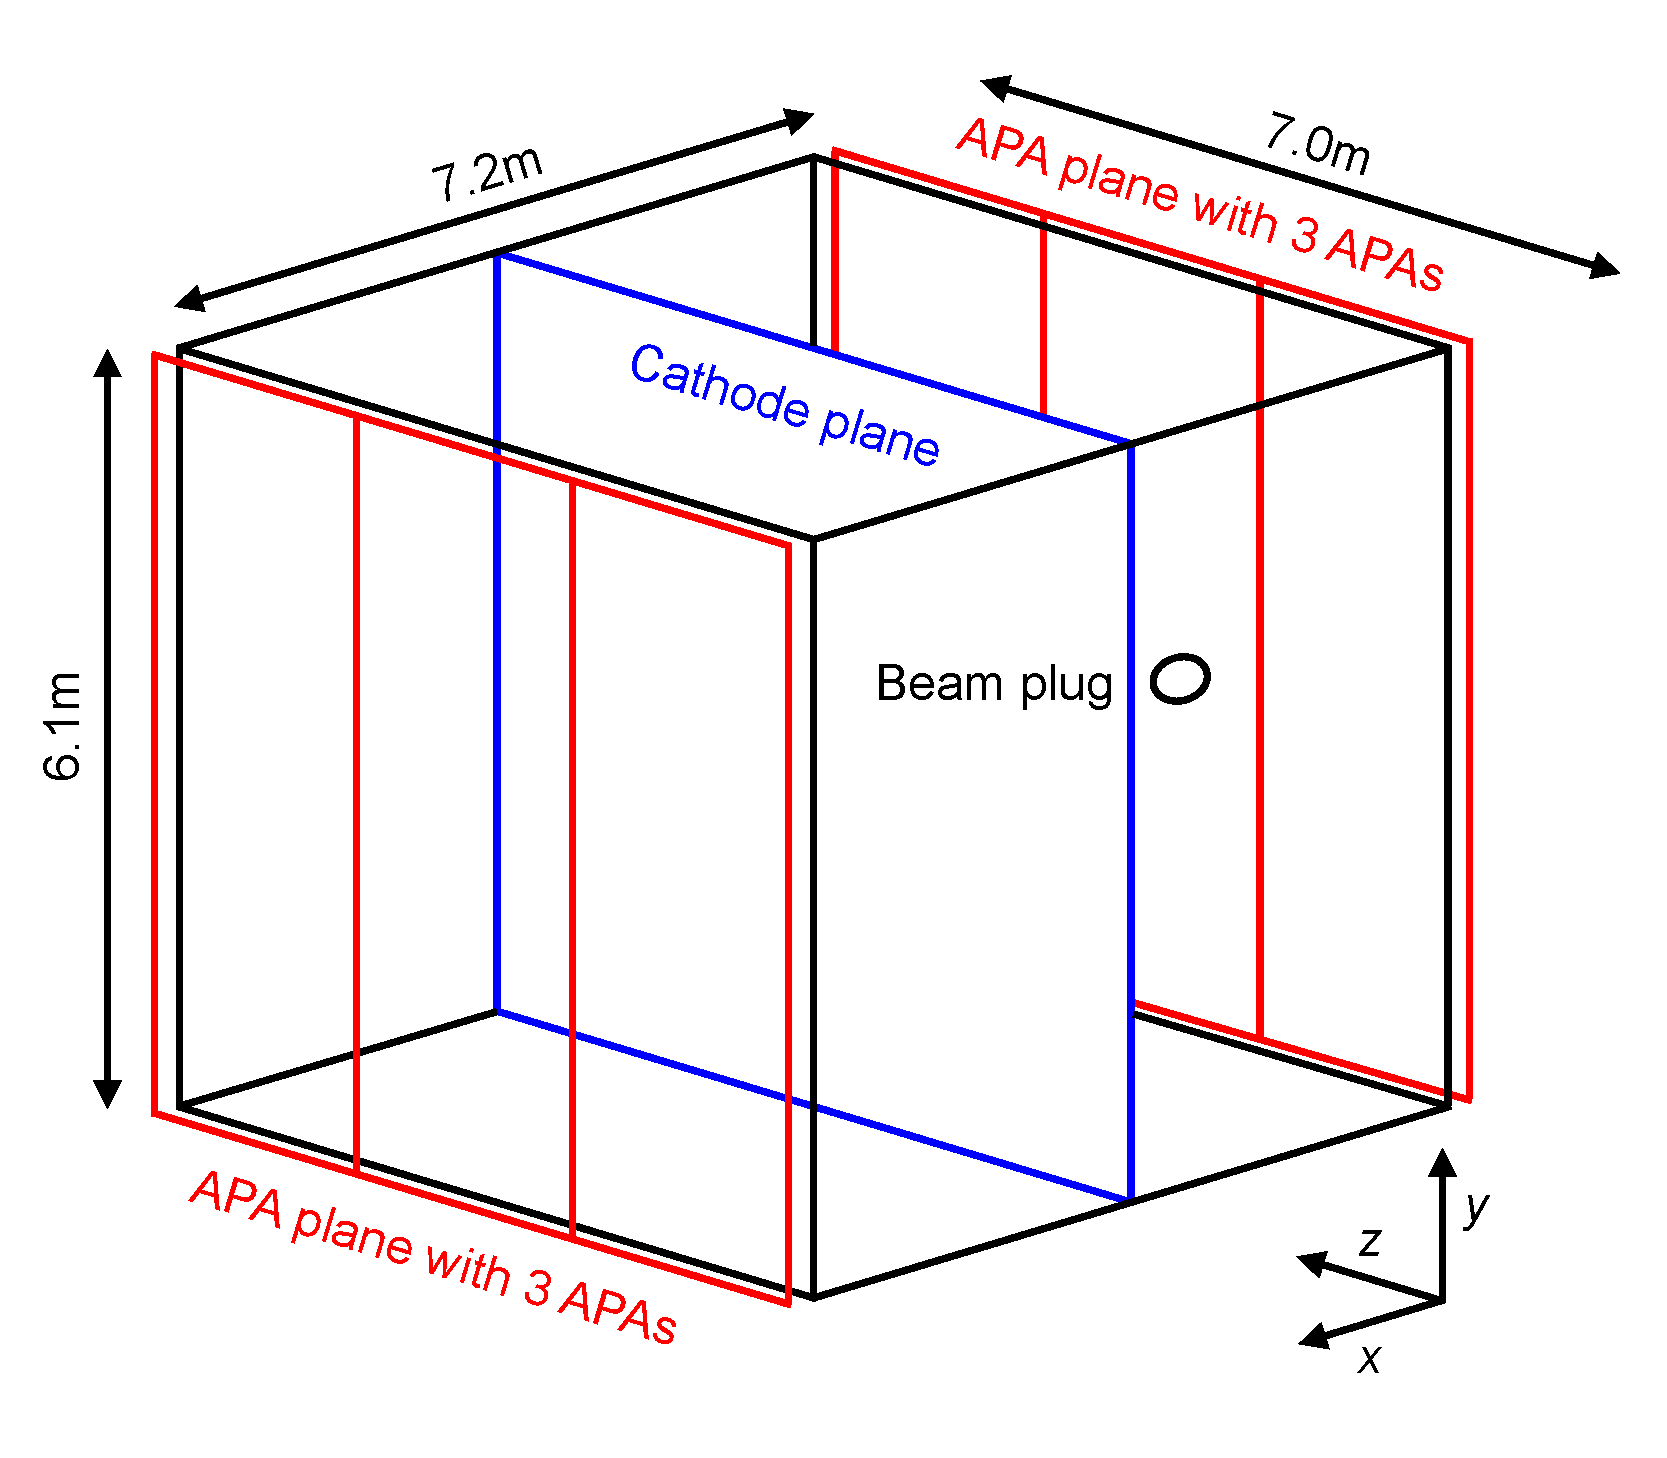
\includegraphics[width=0.48\textwidth]{Figures/Diagram/Schematic_3D.pdf}
    \caption{A simple drawing of the ProtoDUNE-SP detector. The black box represents the active volume, divided into two parts by the central cathode (blue). The six APAs are arranged into two planes (red) either side of the cathode. The test beam enters through the beam plug, close to the right side of the cathode. The right-handed coordinate system is shown in addition to the dimensions of the active volume.}
    \label{fig:schematic3D}
\end{figure}

% Put this figure before it is mentioned in the text to make LaTeX put it where we want it
\begin{figure*}[htb]
\centering
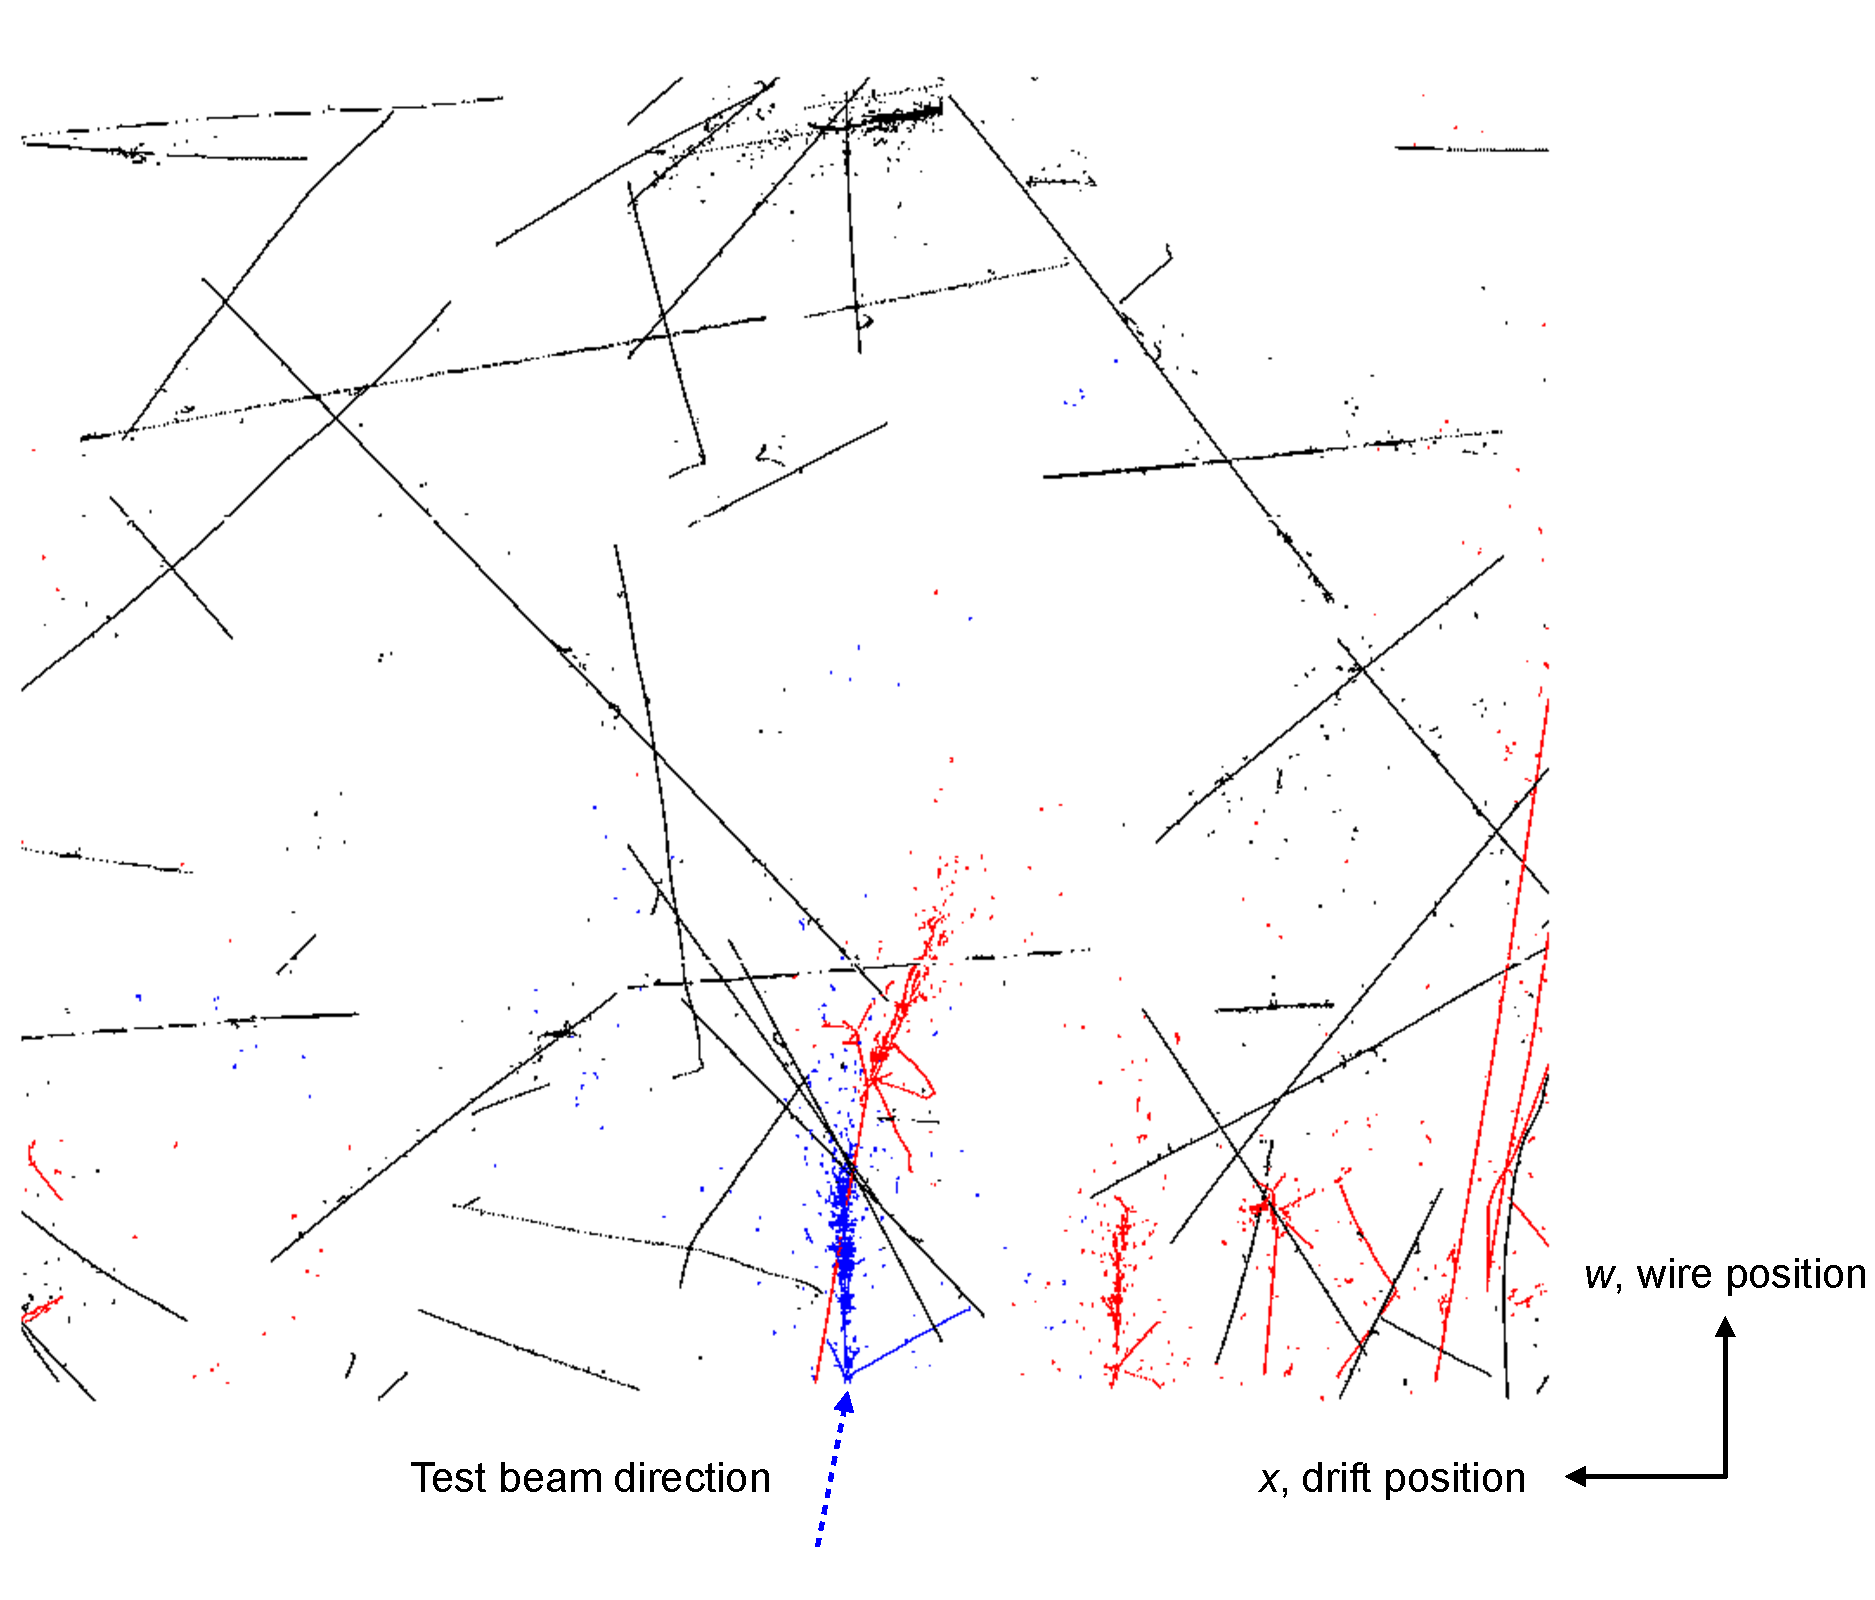
\includegraphics[width=0.8\textwidth]{Figures/EventDisplays/MC/EventComposition.pdf}
\caption{An example of the $w$ view for a simulated 7\,GeV/$c$ $\pi^{+}$ event at ProtoDUNE-SP where the hits have been coloured to indicate their origin: triggered test-beam particle (blue), beam halo (red) and cosmic-ray muon (black). The vertical axis is equivalent to the $z$ axis of the detector and the horizontal axis is converted from the drift time. The test beam particles enter from the upstream end (bottom of the image).}
\label{fig:eventdecomp}
\end{figure*}

A right-handed Cartesian coordinate system was used to describe the detector geometry: $x$ defines the drift axis and is either equal to or opposite to the drift direction, $y$ is the upwards vertical direction and $z$ the remaining orthogonal direction. The test beam was directed primarily along the positive $z$ direction. The origin of the coordinate system is at the bottom of the upstream end of the cathode.

Each wire measures the induced or collected charge as a function of time for the duration of each 3\,ms readout window. The maximal drift time, defined as the time taken for charge to drift from the cathode to the APAs, is approximately 2250\,$\upmu$s. The 3\,ms readout window, relative to the beam trigger time, spans the range from $-$250\,$\upmu$s to 2750\,$\upmu$s and ensures that any charge deposited in the detector at the beam trigger time will be collected. Various detector effects are removed to reduce noise from the raw waveforms. This process consists of the mitigation of noisy readout wires, the removal of coherent and high-frequency noise from the wire signals and the deconvolution of the wire signals. The deconvolution procedure identifies and accounts for signals on a given wire that are produced via induction when adjacent wires observe charge~\cite{wirecell,uBooNESignal}. Hits are then formed from the collected or induced charge waveforms by fitting Gaussian functions to peaks in the waveforms. Each wire plane yields a 2D image of particle interactions in the LArTPC that forms the input to the pattern-recognition algorithms. A full description of signal processing, noise removal and charge calibration is given in Ref.~\cite{proto_performance}.

Figure~\ref{fig:eventdecomp} shows the reconstructed hits for a typical simulated 3\,ms readout window in ProtoDUNE-SP in the collection ($w$) view in the (drift coordinate, wire position) parameter space. For the $w$ view, the wire position is the same as the $z$ coordinate, and the drift time has been converted to the spatial $x$ coordinate using the drift velocity. The three colours represent hits from three classes of particles (and any subsequent particles produced in their interactions): blue shows the \textit{triggered test-beam} 7\,GeV/$c$ charged pion particle that initiated the readout of the detector and interacted almost immediately after entering the TPC; red shows all other beam particles, henceforth called \textit{beam halo} particles, which includes particles from interactions in the beam line, those not focused by the beam-line magnets due to their momentum, particle decays, and focused particles that arrived within the readout window of the triggered beam particle; and black shows cosmic rays (mostly muons). In general, test-beam particle interactions produce complex particle hierarchies (containing secondary, tertiary, etc, particles from interactions and decays) involving both track-like and shower-like energy deposits, while cosmic-ray muons produce highly track-like topologies. Due to the surface location of ProtoDUNE-SP, the majority of the collected charge signals originated from cosmic-ray muons that traverse the detector throughout the 3\,ms readout window. The measured time of charge collected on the wires, $t_m$, is a function of the time that the particle entered the detector ($t_0$) relative to the time that the detector readout was triggered ($t_\textrm{trigger}$), and the distance in the drift coordinate from the APA where the energy was deposited ($x_0$):
\begin{linenomath*}
\begin{equation}
\label{eq:ambiguity}
    t_m = t_0 - t_\textrm{trigger} + x_0/v_d,
\end{equation}
\end{linenomath*}
where $v_d$ is the electron drift velocity. By definition in ProtoDUNE-SP, the trigger time $t_\textrm{trigger} = 0$ and at the nominal electric field the electron drift velocity is $v_d$ = 1.59\,mm/$\upmu$s~\cite{proto_performance}.

Equation \ref{eq:ambiguity} shows that there is an ambiguity between $t_0$ and $x_0$ unless $t_0$ is known. For the test-beam particle that triggers the TPC readout $t_0 = t_\textrm{trigger}$ by definition and there is no ambiguity. In all other cases, the $t_0$ for any particle is initially undetermined and is assumed to arrive at the beam trigger time and hence assigned a preliminary value of $t_0=0$. The exact position inside the TPC where charge was physically deposited is thus only well known for triggered test-beam particles. For other particles (cosmic rays and beam-halo particles) this intrinsic ambiguity in the drift coordinate makes it initially impossible to distinguish between charge deposited by a particle arriving before the beam trigger but far from the APA, and charge deposited by a particle arriving after the beam trigger but close to the APA, since in both cases the time at which the charge is collected by the readout wires would be the same. Other LArTPCs have demonstrated that this ambiguity can be resolved for some interactions by matching the charge information with precise timing information from a photon detector system~\cite{ubLight1,ubLight2}.

The six APAs are read out independently and give rise to six volumes with drift fields (henceforth referred to as \textit{drift regions}), three on either side of the cathode. Since the APAs are read out on both sides, there are also six small volumes without drift fields between the APAs and the cryostat wall (known as \textit{dummy regions}), where charge can be detected if a particle crosses the APA. Figure~\ref{fig:tpcs} shows how adjacent drift regions (separated by the dashed lines) sharing a common drift direction are concatenated together inside Pandora to form two \textit{drift volumes} (red and blue), and the two sets of dummy regions are also concatenated into \textit{dummy volumes} (cyan and magenta). The drift direction for a given drift region is either along positive or negative $x$ depending on the local cathode and APA orientation. The merged drift volumes allow the pattern recognition to trivially correlate inputs between adjacent (in the $z$ direction) drift regions. 

\begin{figure}[htb]
    \centering
    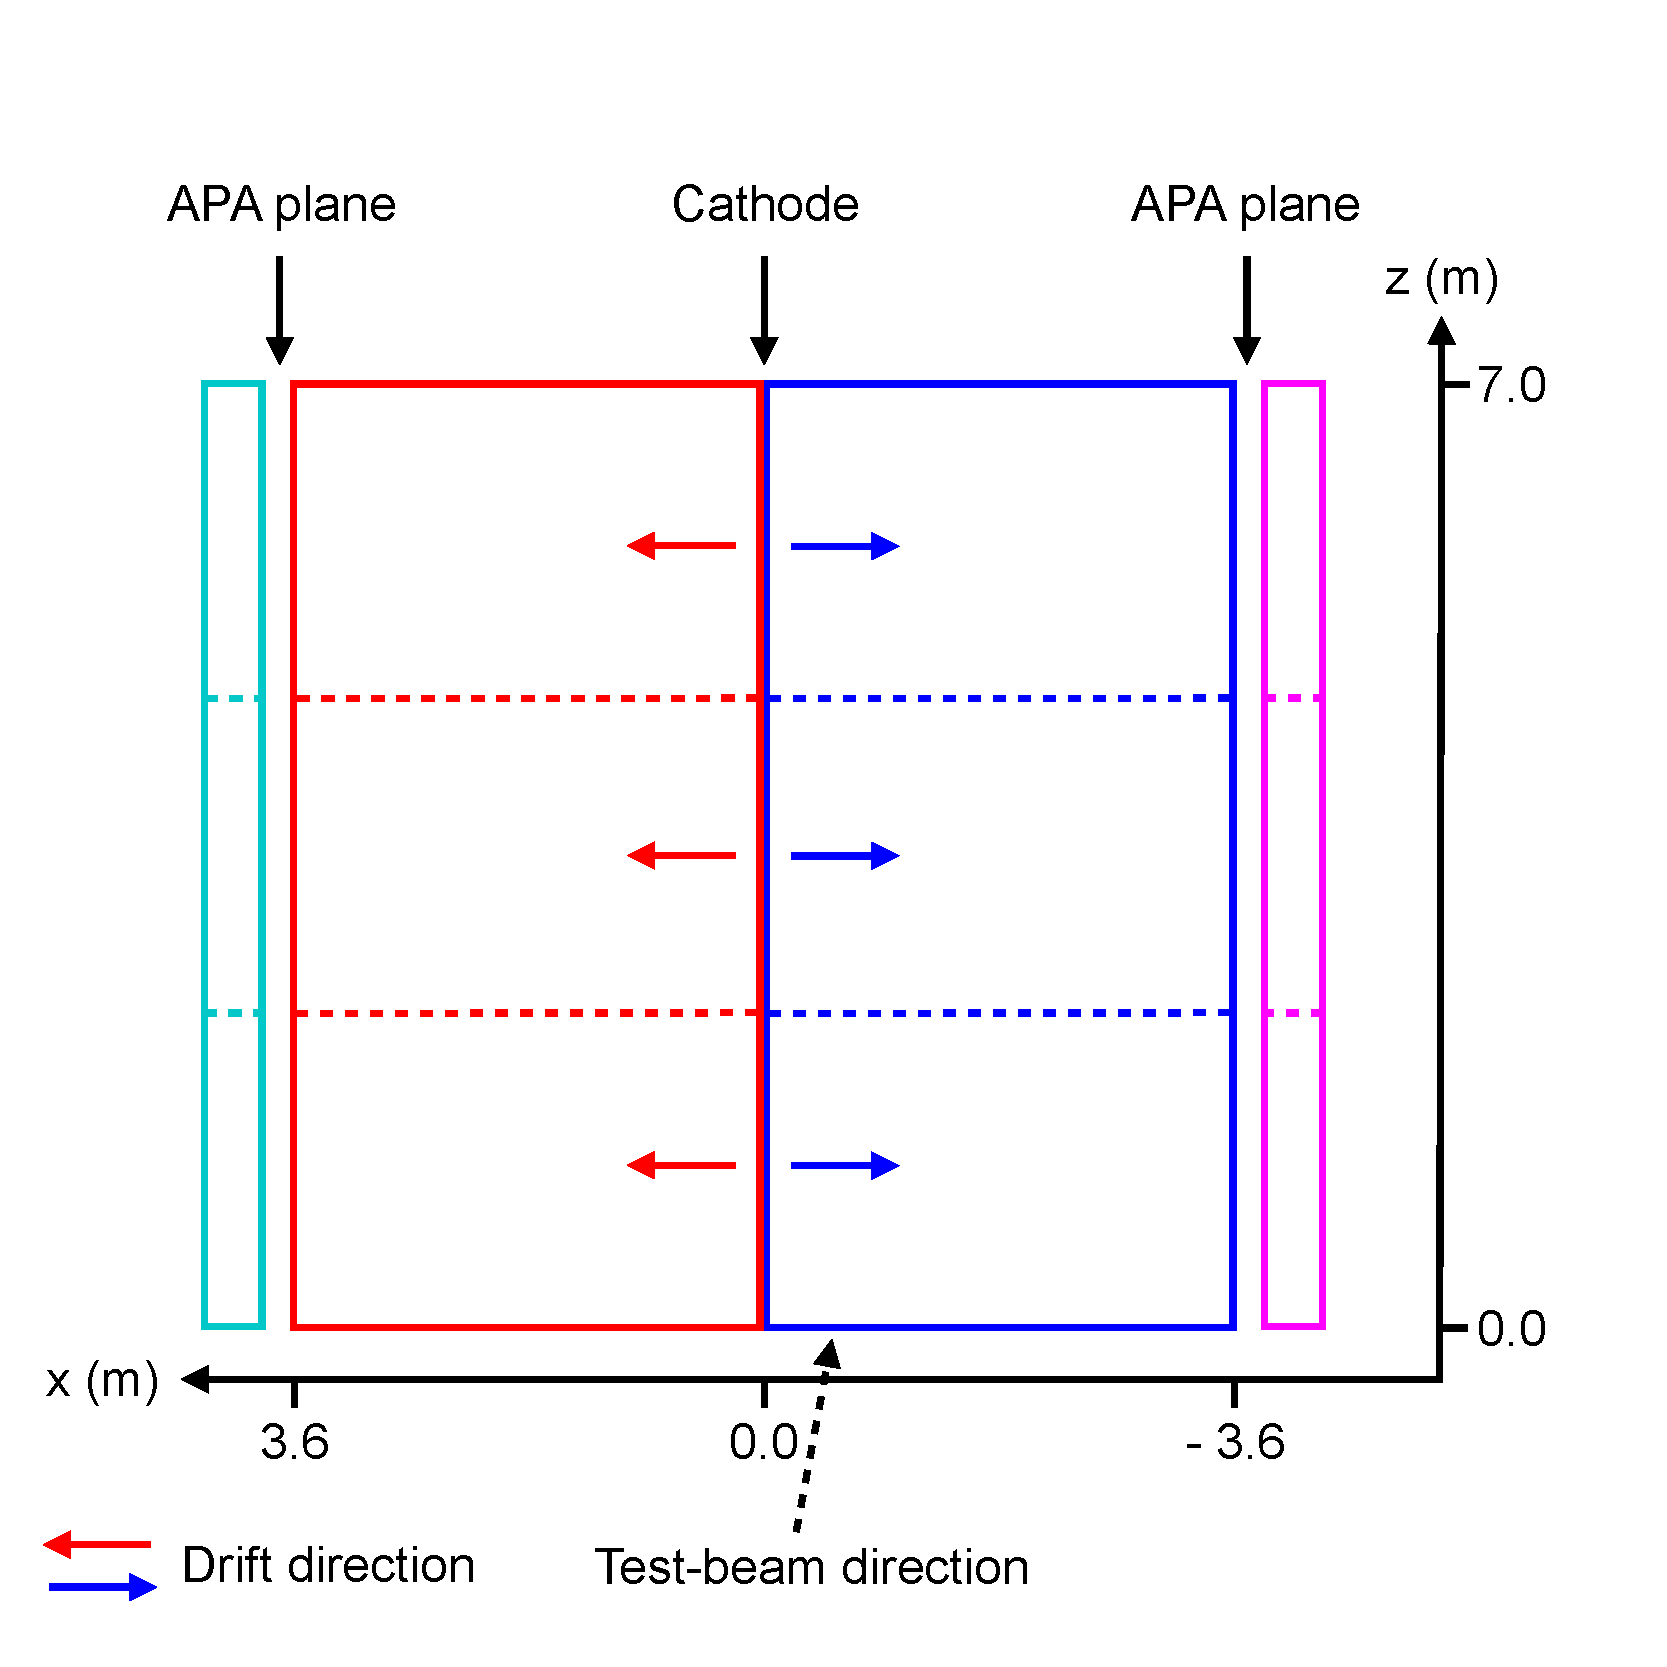
\includegraphics[width=0.48\textwidth]{Figures/Diagram/Schematic_Combined_FromTop.pdf}
    \caption{A schematic top-down view of ProtoDUNE-SP. The six drift regions, each read out by an individual APA, are separated by the dashed lines within the larger drift volumes (red and blue) used inside Pandora. The dummy regions are also combined into dummy volumes (cyan and magenta). The test beam enters the detector close to the cathode and at $z=0$.}
    \label{fig:tpcs}
\end{figure}

\subsection{Space Charge Effects}
Surface-based LArTPC detectors such as ProtoDUNE-SP are subject to space charge effects (SCE): the build up of slow-moving\footnote{Approximately $5\times10^{-5}$mm/$\upmu$s~\cite{ionDrift}} positive ions in the detector due to the high rate of cosmic-ray muons. These ions are produced when charged particles pass through the detector and ionise the liquid argon~\cite{spacecharge}. This effect distorts the electric field by up to 25\% in some regions of the detector and hence the drift velocity of ionisation electrons within the LArTPC. Assuming the nominal uniform electric field, the positions of the reconstructed hits within the detector are shifted with respect to their true positions, and the charges of the hits are also distorted. The simulation uses a data-driven space charge distortion based on measurements of cosmic-ray muons, as described in Ref.~\cite{proto_performance}, which is asymmetric with respect to the cathode. While the SCE is an important consideration for surface detectors, its impact will be much smaller for deep underground detectors such as the DUNE far detectors due to the significantly lower rate of cosmic rays.
 
\section{Pandora Event Reconstruction}
\label{sec:patrec}

The Pandora event reconstruction for ProtoDUNE-SP builds directly upon the approaches and algorithms developed for MicroBooNE, described in Ref.~\cite{pandorauboone}. In this section, the emphasis is on how these algorithms have been carefully extended and harnessed to reconstruct cosmic-ray muon and test-beam particles in a surface-based LArTPC detector comprising multiple drift volumes.

The inputs to the Pandora pattern recognition are hits, and each hit represents a signal detected on a specific wire at a specific time. As at MicroBooNE, the input hits each have a drift time coordinate and a wire coordinate, and each hit is associated with a specific readout plane. This means that three 2D images are presented as inputs: the $u$, $v$ and $w$ views. For ProtoDUNE-SP, one additional piece of information is collected per hit: an index identifying the drift volume from which the hit originates. The wrapping of the induction wires requires that a disambiguation procedure using time-based coincidences between the induction views and the collection view is used to eliminate \textit{ghost} hits. Full details of the disambiguation procedure are given in Ref.~\cite{dunetdr_v2}.

Pandora uses a multi-algorithm approach to pattern recognition, and the three 2D images are considered by a series of over one hundred algorithms and tools, which gradually identify features and build up a picture of events. The final goal is for each given particle to be reconstructed as a single object, that is both pure (containing only hits from that particle) and complete (containing all hits from that particle). Further details are presented in Ref.~\cite{pandorauboone}, but the overall approach is to:

\begin{itemize}
    \item \textbf{Add hits to clusters.} The hits from each readout plane are considered separately and clustered, with the aim of creating one cluster per input particle. This procedure begins with a main clustering algorithm that is designed to be conservative to prioritise making pure but incomplete clusters and avoiding mistakes. A series of subsequent ``topological association'' algorithms exploit the detector granularity to increase the cluster completeness, whilst maintaining purity.
    \item \textbf{Add clusters to particles.} The clusters from each readout plane are carefully compared, by exploiting the drift coordinate common to all planes, and by using knowledge of the wire angles to correlate features in 3D. By comparing the independent 2D pattern-recognition outcomes for the three planes, corrections to the 2D clustering can be made, and clusters can be unambiguously associated between planes. Clusters are bound together to form reconstructed particles.
    \item \textbf{Add particles to hierarchies.} Reconstructed particles contain clusters from two or more readout planes, allowing a list of 3D hits to be created for each. A series of further topological association algorithms (now operating in 3D) continue to grow particle completeness, without sacrificing purity. The reconstruction concludes by organising the final particles into a 3D hierarchy, representing the final state particles and any subsequent interactions or decays.
\end{itemize}

For MicroBooNE, two chains of Pandora algorithms were created to reconstruct the input images under the hypothesis that the inputs were cosmic-ray muons (the PandoraCosmic chain), or under the hypothesis that the inputs represented the final state particles emerging from a neutrino interaction (the PandoraNu chain).

In this section, details are presented of how the PandoraCosmic chain has been adapted for a detector with multiple drift volumes. Details are then presented of how the PandoraNu chain has been adapted to represent the interactions of charged particles in a test beam (and renamed PandoraTestBeam). Finally, a description is provided of how these two algorithm chains have been carefully woven together to provide a clear reconstruction output. The aim is to provide an unambiguous interpretation of the input hits at ProtoDUNE-SP as a list of identified cosmic-ray muon hierarchies and a list of identified test-beam particle hierarchies. This ``consolidated'' reconstruction is a refinement of the two-pass approach previously documented.

\subsection{PandoraCosmic}
\label{sec:pandoracosmic}

The PandoraCosmic algorithm chain was developed to provide a highly efficient reconstruction of cosmic-ray muon trajectories. Following the initial track-like clustering and particle-creation algorithms, any remaining hits are used to seed and grow shower particles. Parent track particles, representing the muons, are linked to child shower particles, representing Michel electrons or delta rays. The muons are assumed to be downward going, so their primary vertices are placed at their highest reconstructed $y$ coordinates.

Cosmic rays arrive throughout the detector readout window. As previously mentioned, all hits passed to the pattern recognition are placed assuming that they correspond to a particle arriving at $t_0=t_\textrm{trigger}$. For cosmic rays, this can result in a shift in the drift coordinate at which their hits are placed. For trajectories contained within a single drift volume, there is a constant offset in the drift time coordinate. This offset may place the hits outside of the physical drift volume, and this is useful information for tagging particles that are not the triggered test-beam particle.

The ProtoDUNE-SP detector has four adjacent volumes (the two central drift volumes and the two outer dummy volumes), which gives the potential for cosmic-ray muons to cross between volumes, and this provides new information and a new challenge. The hits from one muon (arriving at a time offset from the trigger time) will be shifted in each volume. But, as the drift direction alternates between adjacent volumes, their drift coordinates will be shifted in opposite directions. In the reconstruction, each drift volume is initially processed in isolation, resulting in separately reconstructed 3D particles in each volume. The separate particles are shifted by equal amounts from the cathode, but the direction of the shift alternates between adjacent volumes.

By identifying the relevant reconstructed particles in each drift volume, based on their directions and relative locations in the $y$-$z$ plane, it is possible to identify the arrival time of the underlying particle, and so correct the drift coordinates for the associated hits. Shifting the particles by equal amounts\footnote{There is some tolerance in these shifts between the two track segments to allow for an asymmetric SCE or slight imperfections in the track reconstruction.} (in appropriate directions) in the drift coordinate should yield a single trajectory that is continuous in both its position and direction across the boundary between drift volumes. The separate component particles can then be \textit{stitched} together. The $t_0$ corrections identified by this stitching process allow for a single coherent 3D particle trajectory to be reconstructed, as demonstrated in Fig.~\ref{fig:stitching}. Performance metrics assessing the stitching performance and a discussion of how the SCE affects the measured $t_0$ are presented in Sec.~\ref{sec:crmetrics}.

\begin{figure}[htb]
\centering
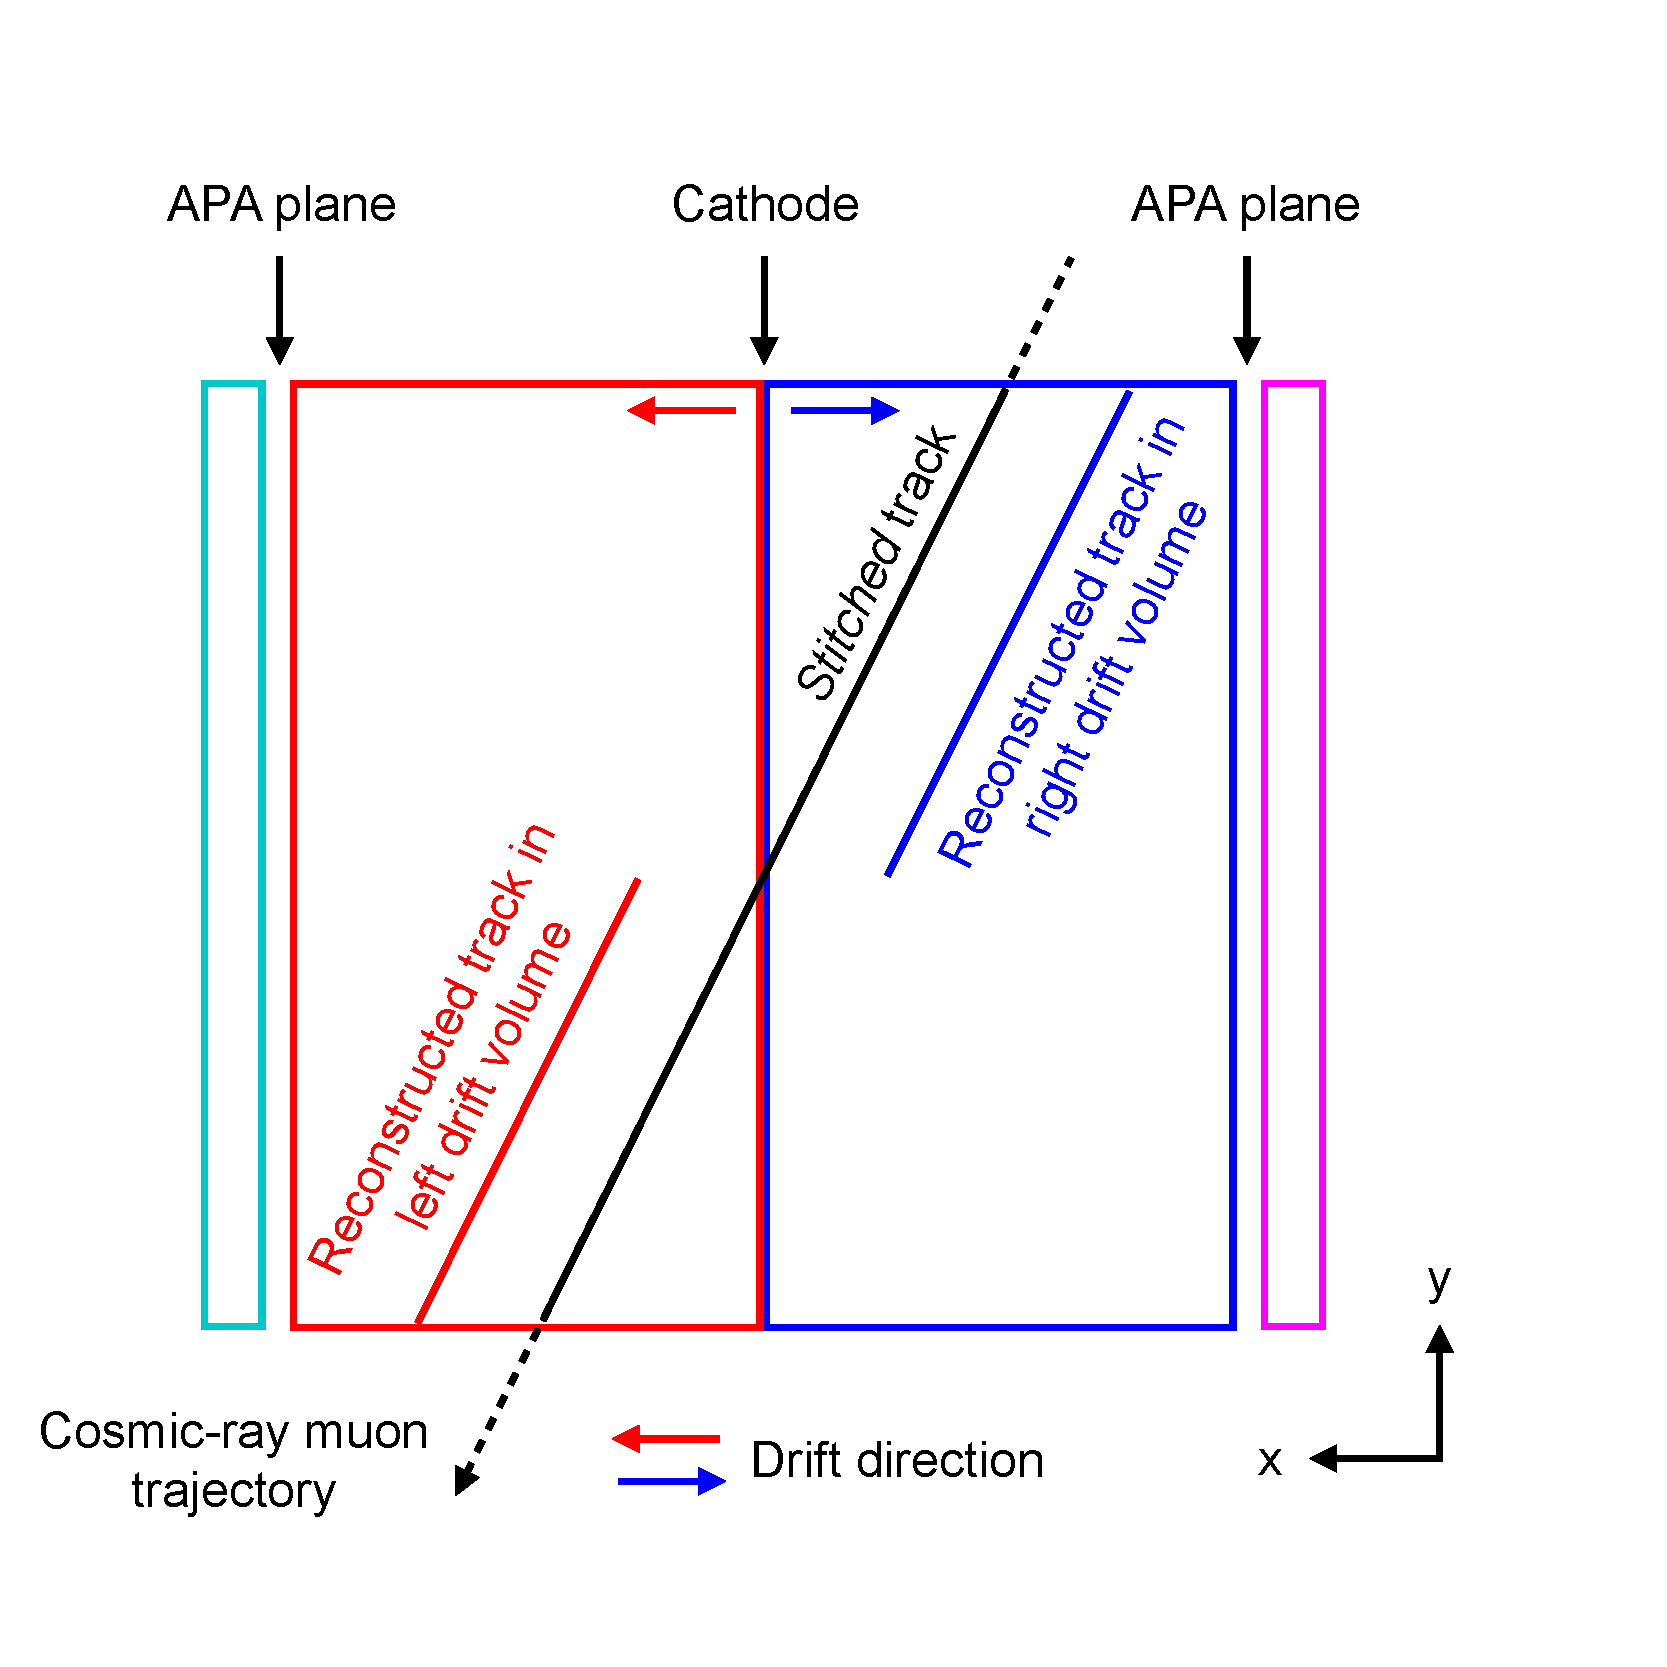
\includegraphics[width=0.48\textwidth]{Figures/EventDisplays/Stitching/Stitching_Schematic_FromTop.pdf}
\caption{A sketch of the \textit{stitching} procedure showing a cosmic-ray muon crossing from top-to-bottom in the (x,y) projection. The two initial reconstructed particles (red and blue) have been independently reconstructed in the two central drift volumes. Based on pointing information and consistent $y$-$z$ coordinates, they have been identified as parts of the same cosmic-ray muon and merged to form the black particle after applying a shift in drift position to each of the two initial reconstructed particles.}
\label{fig:stitching}
\end{figure}

\subsection{PandoraTestBeam}
\label{sec:pandoratestbeam}

The PandoraTestBeam algorithm chain is a modified version of the PandoraNu chain presented in Ref.~\cite{pandorauboone}. This chain focuses on identifying an interaction vertex, and reconstructing the individual track-like and shower-like particles that emerge from this point. Many of the algorithms are shared with the PandoraCosmic chain, but the vertex identification algorithms are specific to this chain, and there is a more sophisticated treatment of electromagnetic showers. The chain concludes with algorithms to build a hierarchy, representing the particle flow in the interaction. The hierarchy is initially built under the preexisting neutrino hypothesis: a parent particle has child particles that represent the final-state particles emerging from the interaction point, and these may themselves have further child particles.

PandoraTestBeam diverges from PandoraNu only in its final stages, after an initial hierarchy of particles has been constructed. A new test-beam particle creation algorithm reorganises the hierarchy as appropriate for the interaction of an incoming charged test-beam particle. Particles initially reconstructed as emerging from the interaction vertex are reconsidered and the particle that is most consistent with actually being an \textit{incoming} particle is identified. The reconstructed placeholder parent particle is replaced with this identified primary beam particle, which has both reconstructed start and interaction vertices. The parent-child links in the hierarchy are repackaged to represent the newly-identified particle flow. Figure~\ref{fig:testbeamcreation} shows an example reconstructed particle hierarchy for a simulated test-beam proton interaction.

\begin{figure}[tb]
\centering
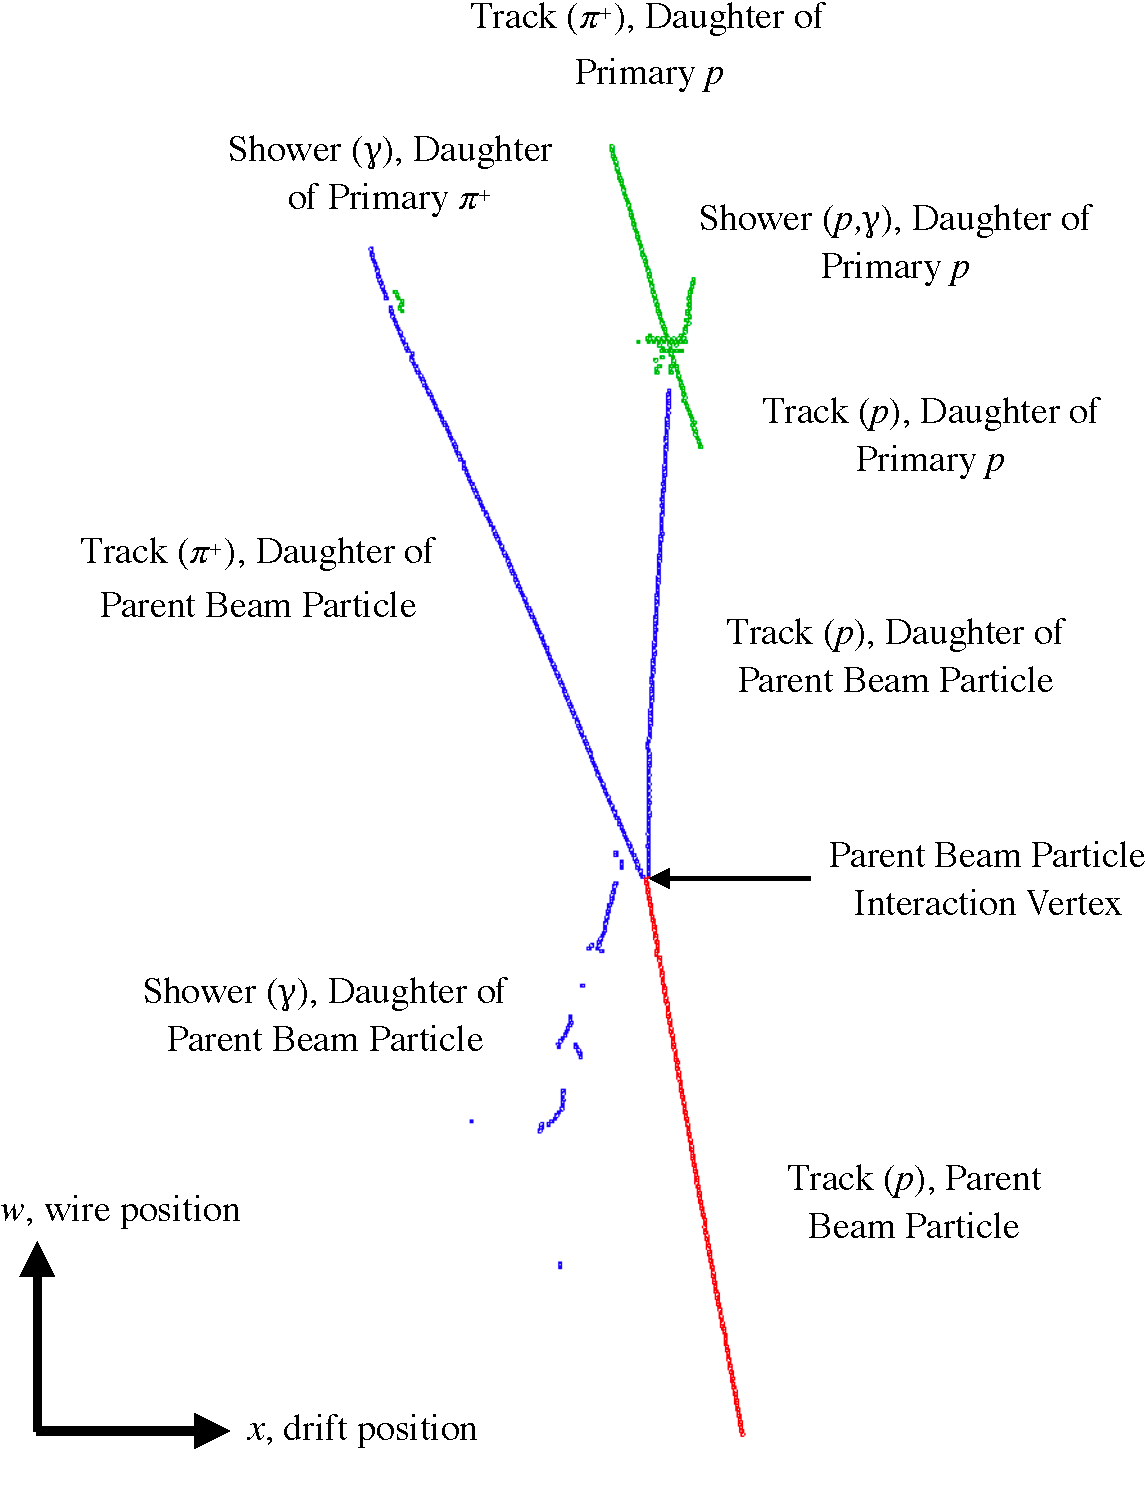
\includegraphics[width=0.45\textwidth]{Figures/EventDisplays/MC/TestBeamParticleCreation.pdf}
\caption{An example of the 2D reconstruction output for a triggered test-beam particle. The particle hierarchy has been reconstructed to reflect the presence of an incoming track-like parent particle. The parent particle (red), child particles (blue) and subsequent child particles (green) have been separately highlighted.}
\label{fig:testbeamcreation}
\end{figure}

\subsection{Consolidated Reconstruction}
\label{sec:consolidatedreconstruction}

A detector readout window contains energy deposits from a number of cosmic rays, and perhaps from beam halo particles and a triggered beam particle. The aim of the Pandora consolidated reconstruction approach is to have one process that intelligently uses the PandoraCosmic and PandoraTestBeam algorithm chains so as to provide a clear and easy-to-interpret reconstruction output, with no double counting of any input hits. The output is a number of tagged reconstructed cosmic-ray particle hierarchies and a number of tagged reconstructed test-beam particle hierarchies. A flow diagram illustrating the consolidated reconstruction approach is shown in Fig.~\ref{fig:consolidatedreco} and the following sections describe the different parts of this combined workflow.

\begin{figure}[tb]
\centering
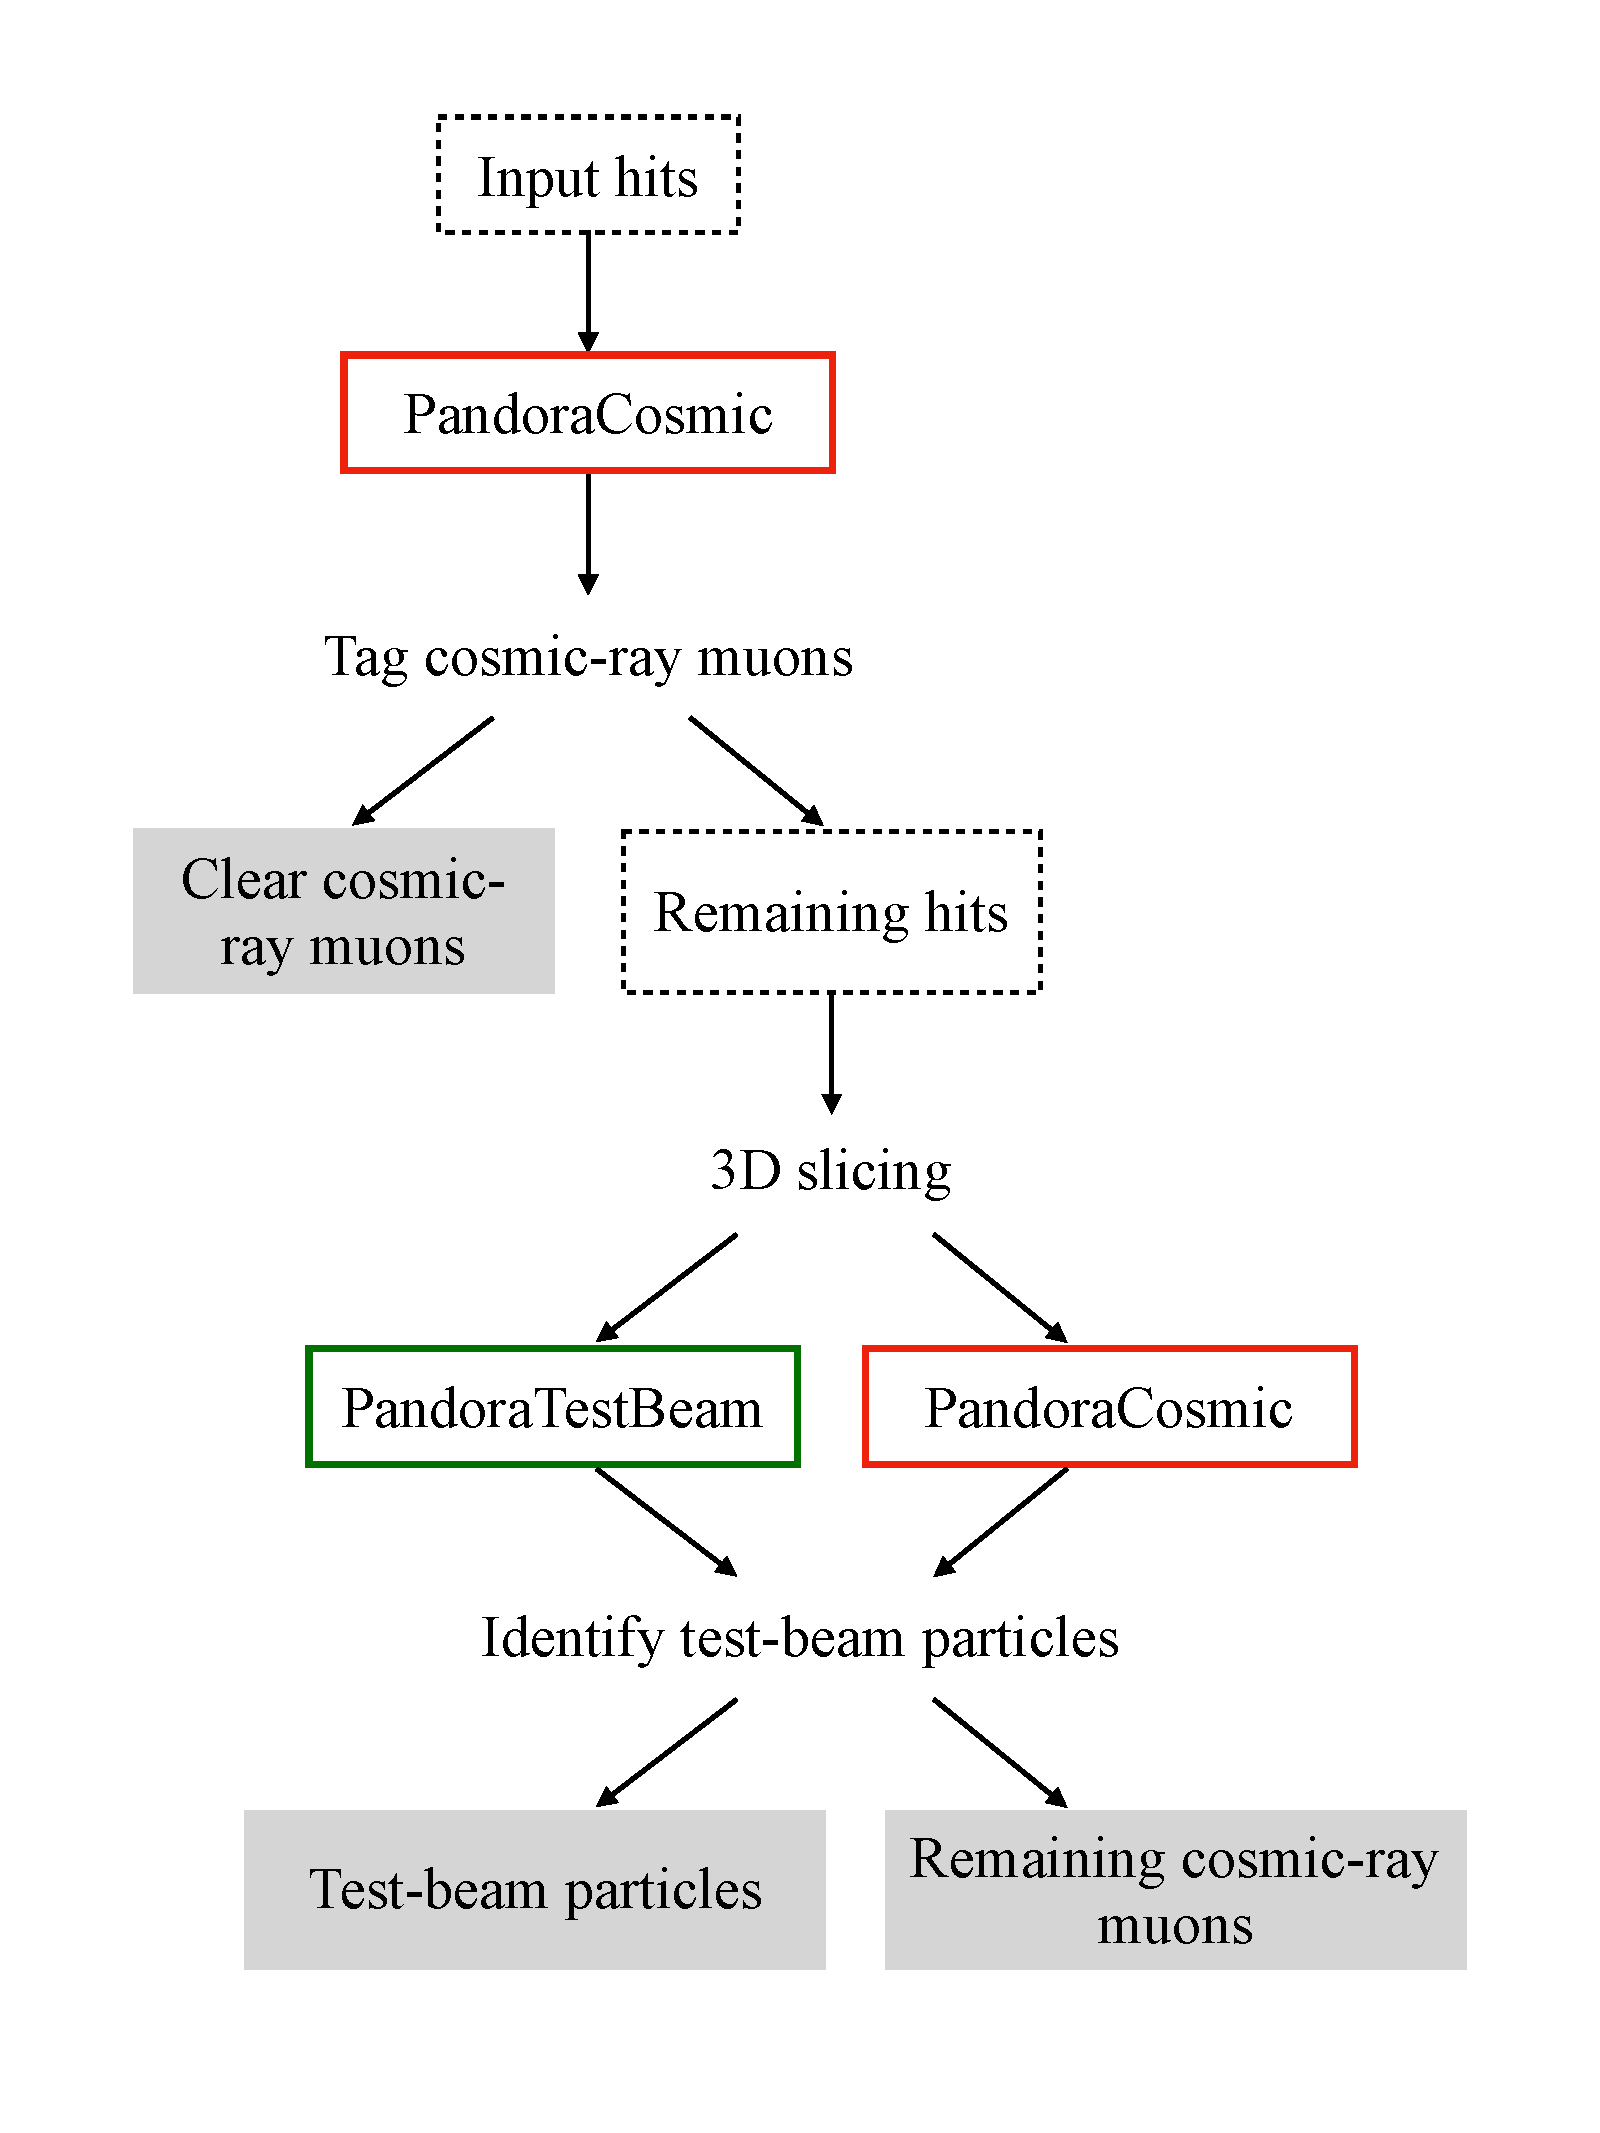
\includegraphics[width=0.45\textwidth]{Figures/Diagram/ConsolidatedReco.pdf}
\caption{Outline of the Pandora consolidated reconstruction. The PandoraTestBeam and PandoraCosmic algorithm chains run on the same hits in a given slice (a region of the detector containing hits originating from a single parent particle interaction) and yield two reconstruction outputs that can be compared and the optimal reconstruction selected.}
\label{fig:consolidatedreco}
\end{figure}

\subsubsection{Cosmic-Ray Muon Reconstruction, Stitching and Tagging}
\label{sec:stitching}
In the first step, hits from the four drift volumes are processed separately using the PandoraCosmic chain. The reconstructed particles from each drift volume then pass through the track stitching algorithm to fully reconstruct those particles that traverse neighbouring drift volumes.


In the next step, the individual cosmic-ray hierarchies are evaluated, and any hierarchies that represent clear cosmic-ray muons are tagged as complete, and removed from subsequent reconstruction steps. At this stage of the reconstruction, any hits from a triggered test-beam particle will also have been processed by the PandoraCosmic algorithm chain. It is important to ensure that these hits are not removed in this step, so that they can later be processed by the PandoraTestBeam chain. Three distinct checks are applied and a reconstructed particle hierarchy is tagged as a clear cosmic-ray muon hierarchy if any of the following are satisfied:

\begin{figure*}[htb]
\centering
\subfloat[]{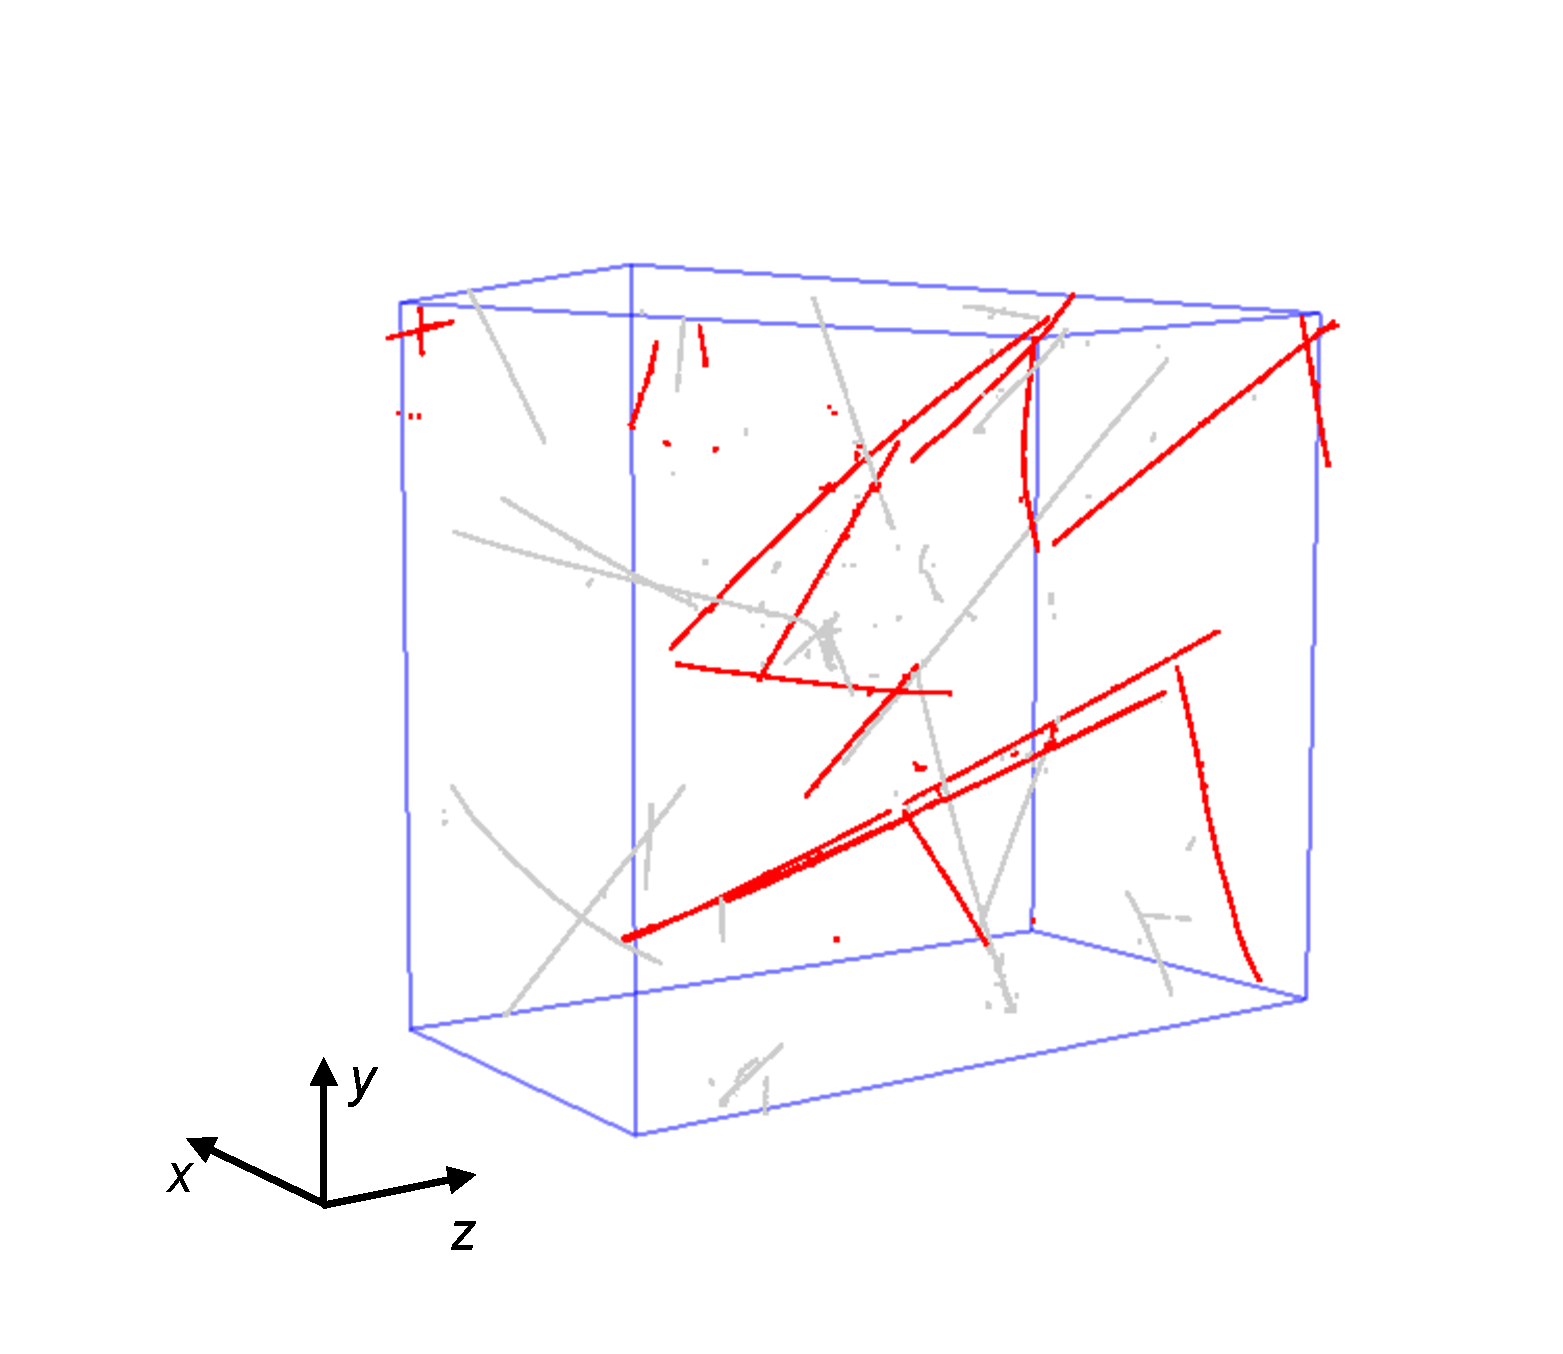
\includegraphics[width=0.42\textwidth,trim={1cm 0 1cm 0},clip]{Figures/Diagram/InTime/cosmic_out_of_time_3D.pdf}\label{fig:intime3d}}
\subfloat[]{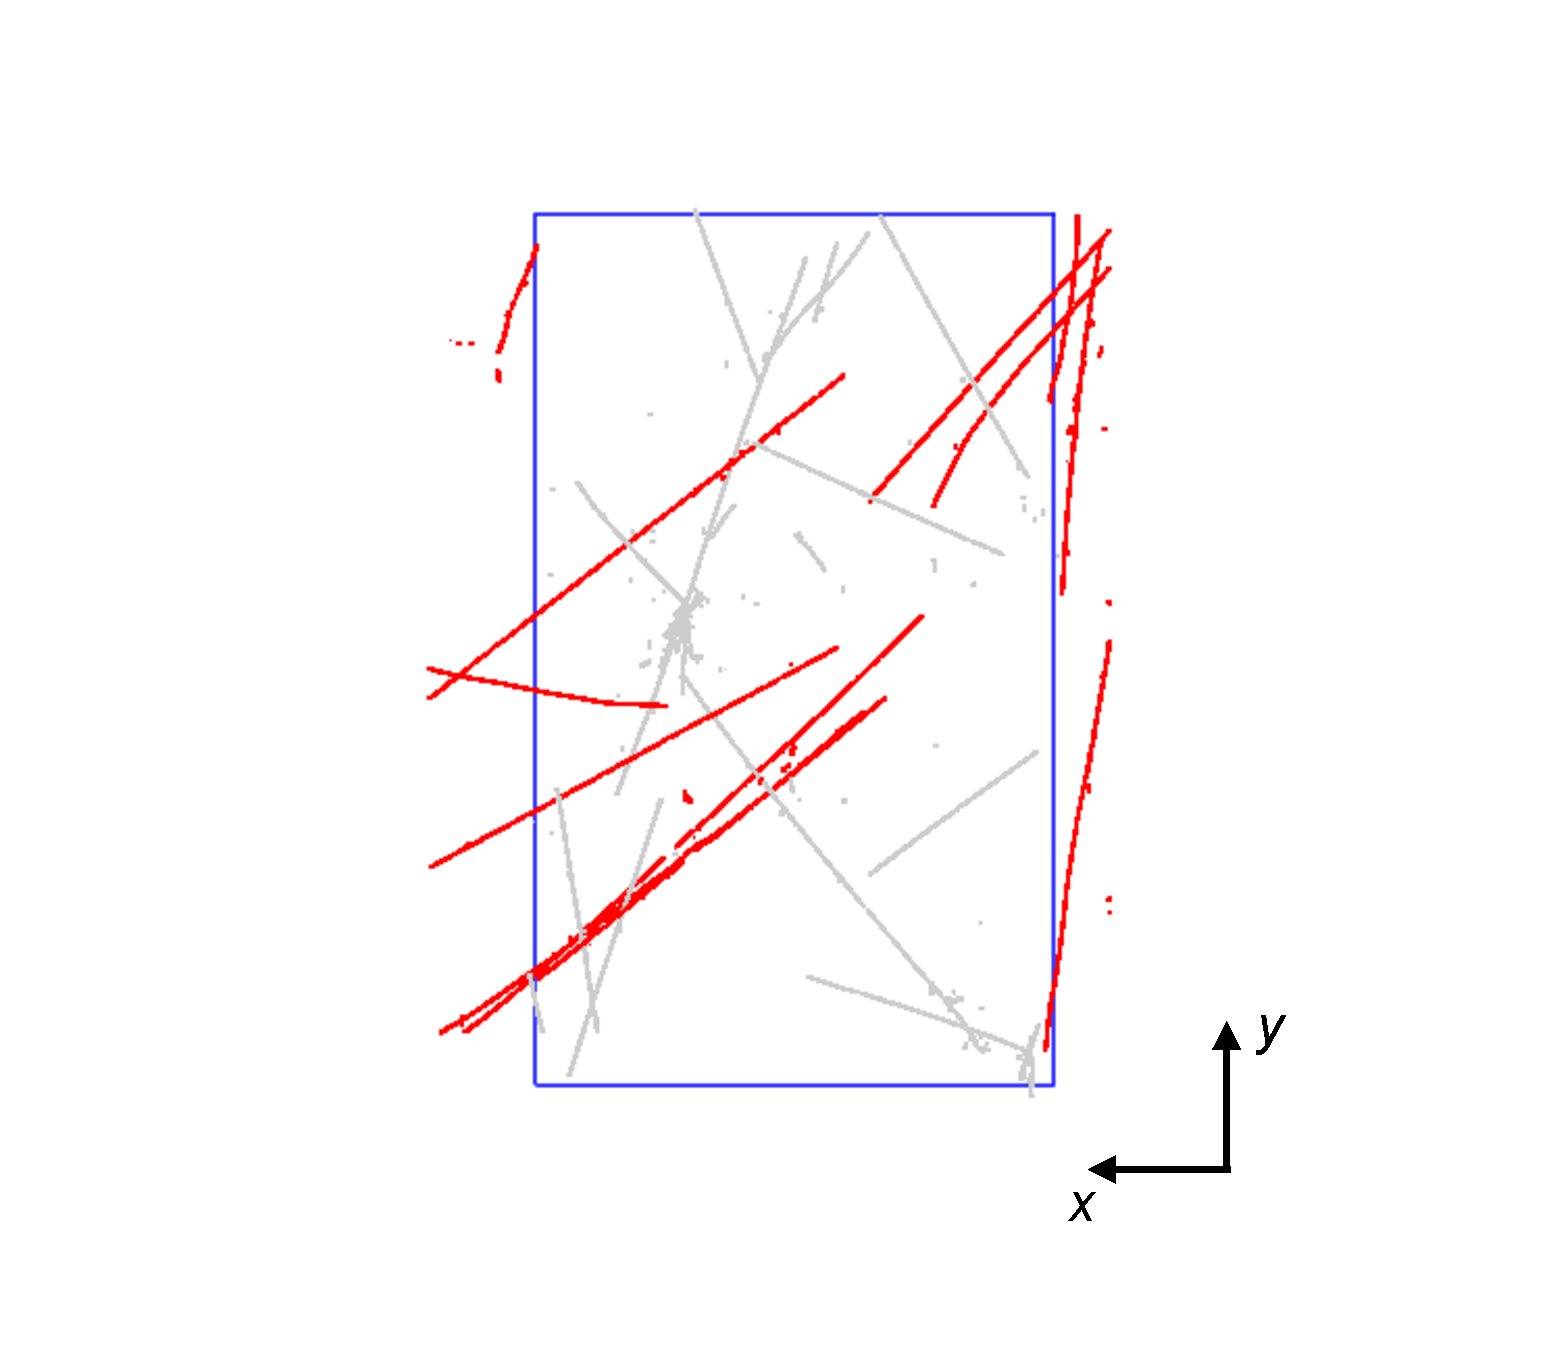
\includegraphics[width=0.28\textwidth,trim={6cm 0 4cm 0},clip]{Figures/Diagram/InTime/cosmic_out_of_time_2D_XY.pdf}\label{fig:intimexy}}
\subfloat[]{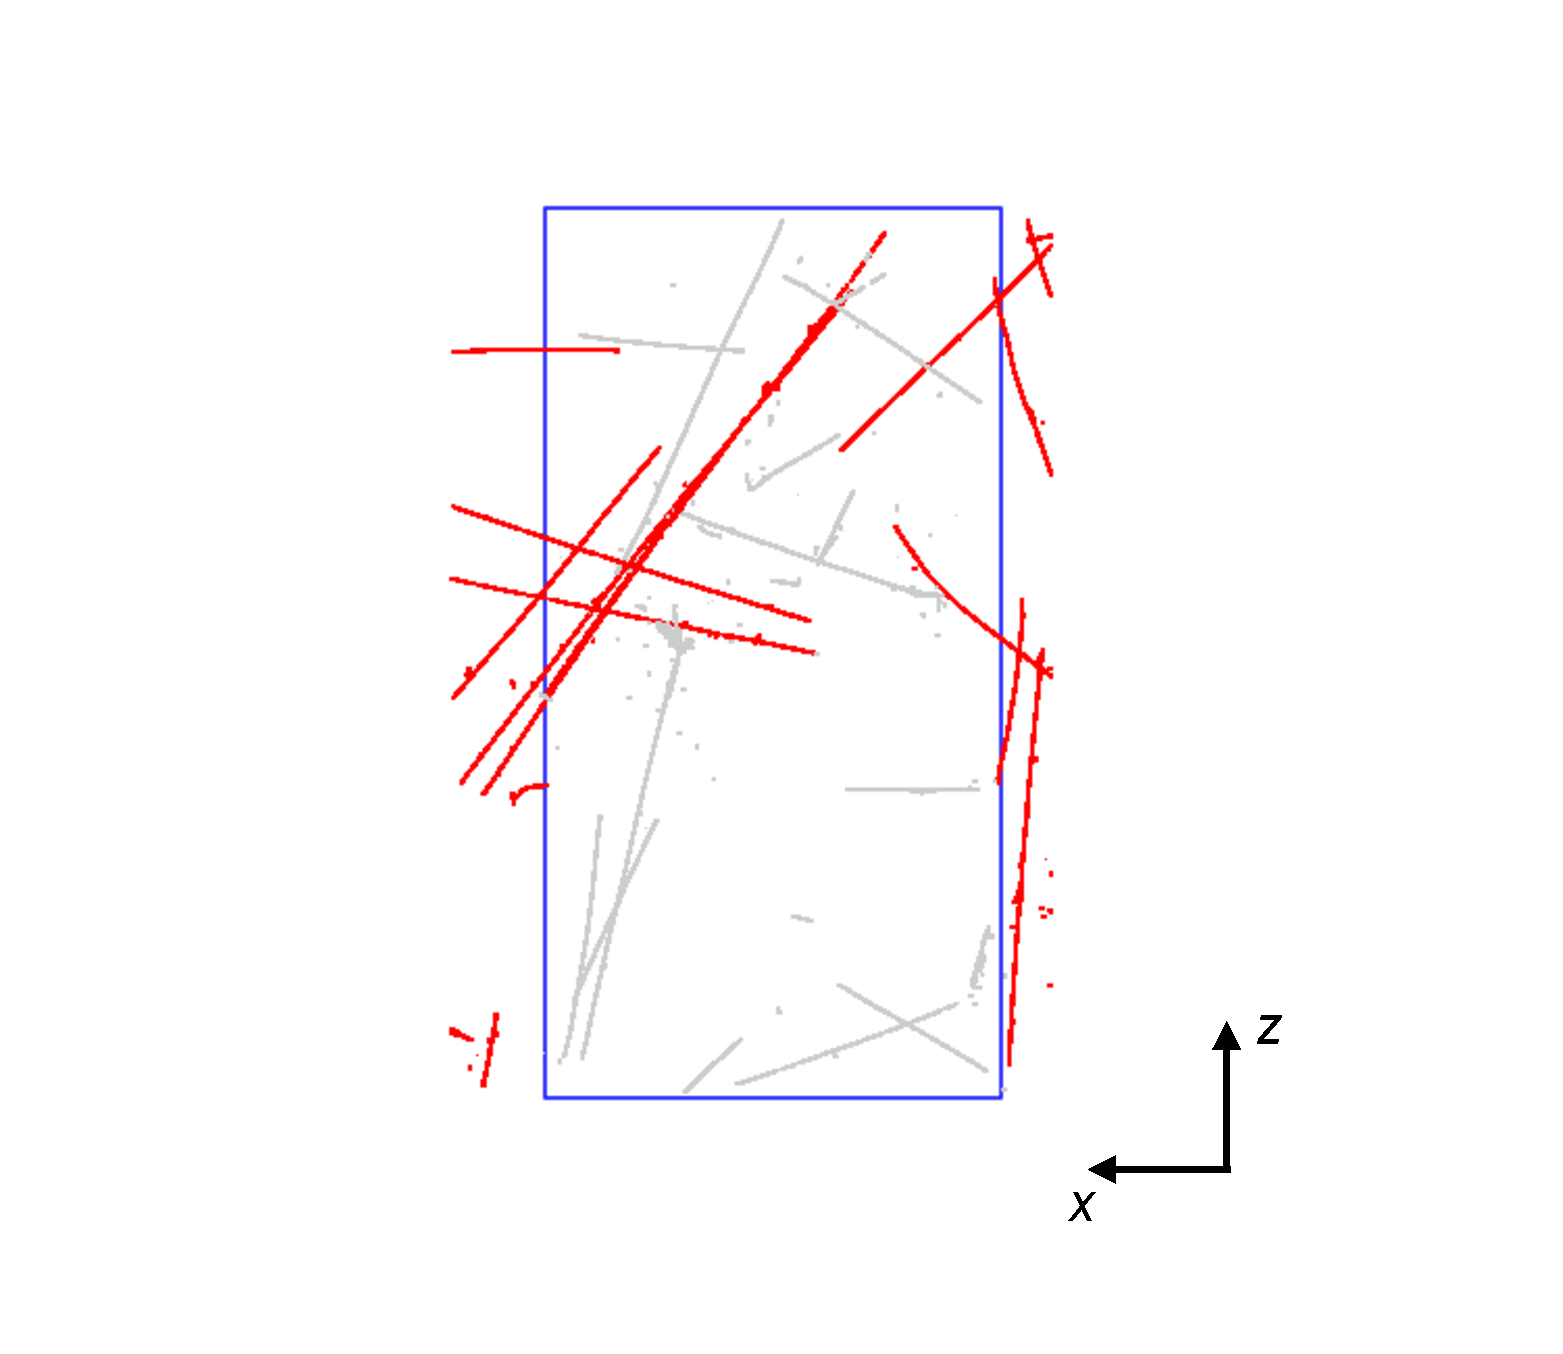
\includegraphics[width=0.28\textwidth,trim={6cm 0 4cm 0},clip]{Figures/Diagram/InTime/cosmic_out_of_time_2D_XZ.pdf}\label{fig:intimexz}}
\caption{The reconstructed output using the PandoraCosmic algorithm chain in \protect\subref{fig:intime3d} 3D, \protect\subref{fig:intimexy} the \textit{x-y} plane and \protect\subref{fig:intimexz} the \textit{x-z} plane for a simulated event in ProtoDUNE-SP. For illustrative purposes, only hits appearing in the beam-side central drift volumes in ProtoDUNE-SP have been reconstructed. Particles in red are deemed to be out of time, as they appear outside the physical boundary of the drift volumes because no offset in the drift position has been applied. Particles in grey are those deemed to be in time. Out-of-time particles are tagged as cosmic-ray muons.}
\label{fig:intime}
\end{figure*}

\begin{itemize}
\item Any hits in the reconstructed particle (placed assuming arrival at the beam trigger time) fall outside of the physical drift volume boundary, as illustrated in Fig.~\ref{fig:intime}.
\item The reconstructed particle was stitched across the cathode or an APA plane and the difference between the reconstructed $t_0$ and the beam trigger time exceeds 6.2\,$\upmu$s, corresponding to a shift of 1\,cm in drift position in the stitching process.
\item The reconstructed particle crosses the top and bottom boundaries of the detector.
\end{itemize}

Reconstructed particle hierarchies tagged as clear cosmic-ray muons are set aside to form one part of the consolidated reconstruction output. The hits that form these clear cosmic-ray muon hierarchies are not considered in the remaining steps of the reconstruction.

\subsubsection{Event Slicing}
The hits remaining after the removal of the clear cosmic-ray muon hierarchies are analysed further. The aim is to divide up the hits into \textit{slices}, where each slice represents an individual true particle hierarchy. For instance, one slice might ideally represent a cosmic-ray muon (including delta-rays and a possible Michel electron), one might represent a beam halo interaction and one might represent a triggered test-beam particle interaction.


A technical detail is that the four drift volumes can now be combined within Pandora. This is because the out-of-time hits have been removed by this stage, so the remaining hits can be considered in the context of one ``global'' drift volume. This volume extends to cover the space occupied by the constituent drift volumes, and any uninstrumented regions at cathode or APA boundaries are registered as detector gaps.

\begin{figure*}[htb]
\centering
\subfloat[]{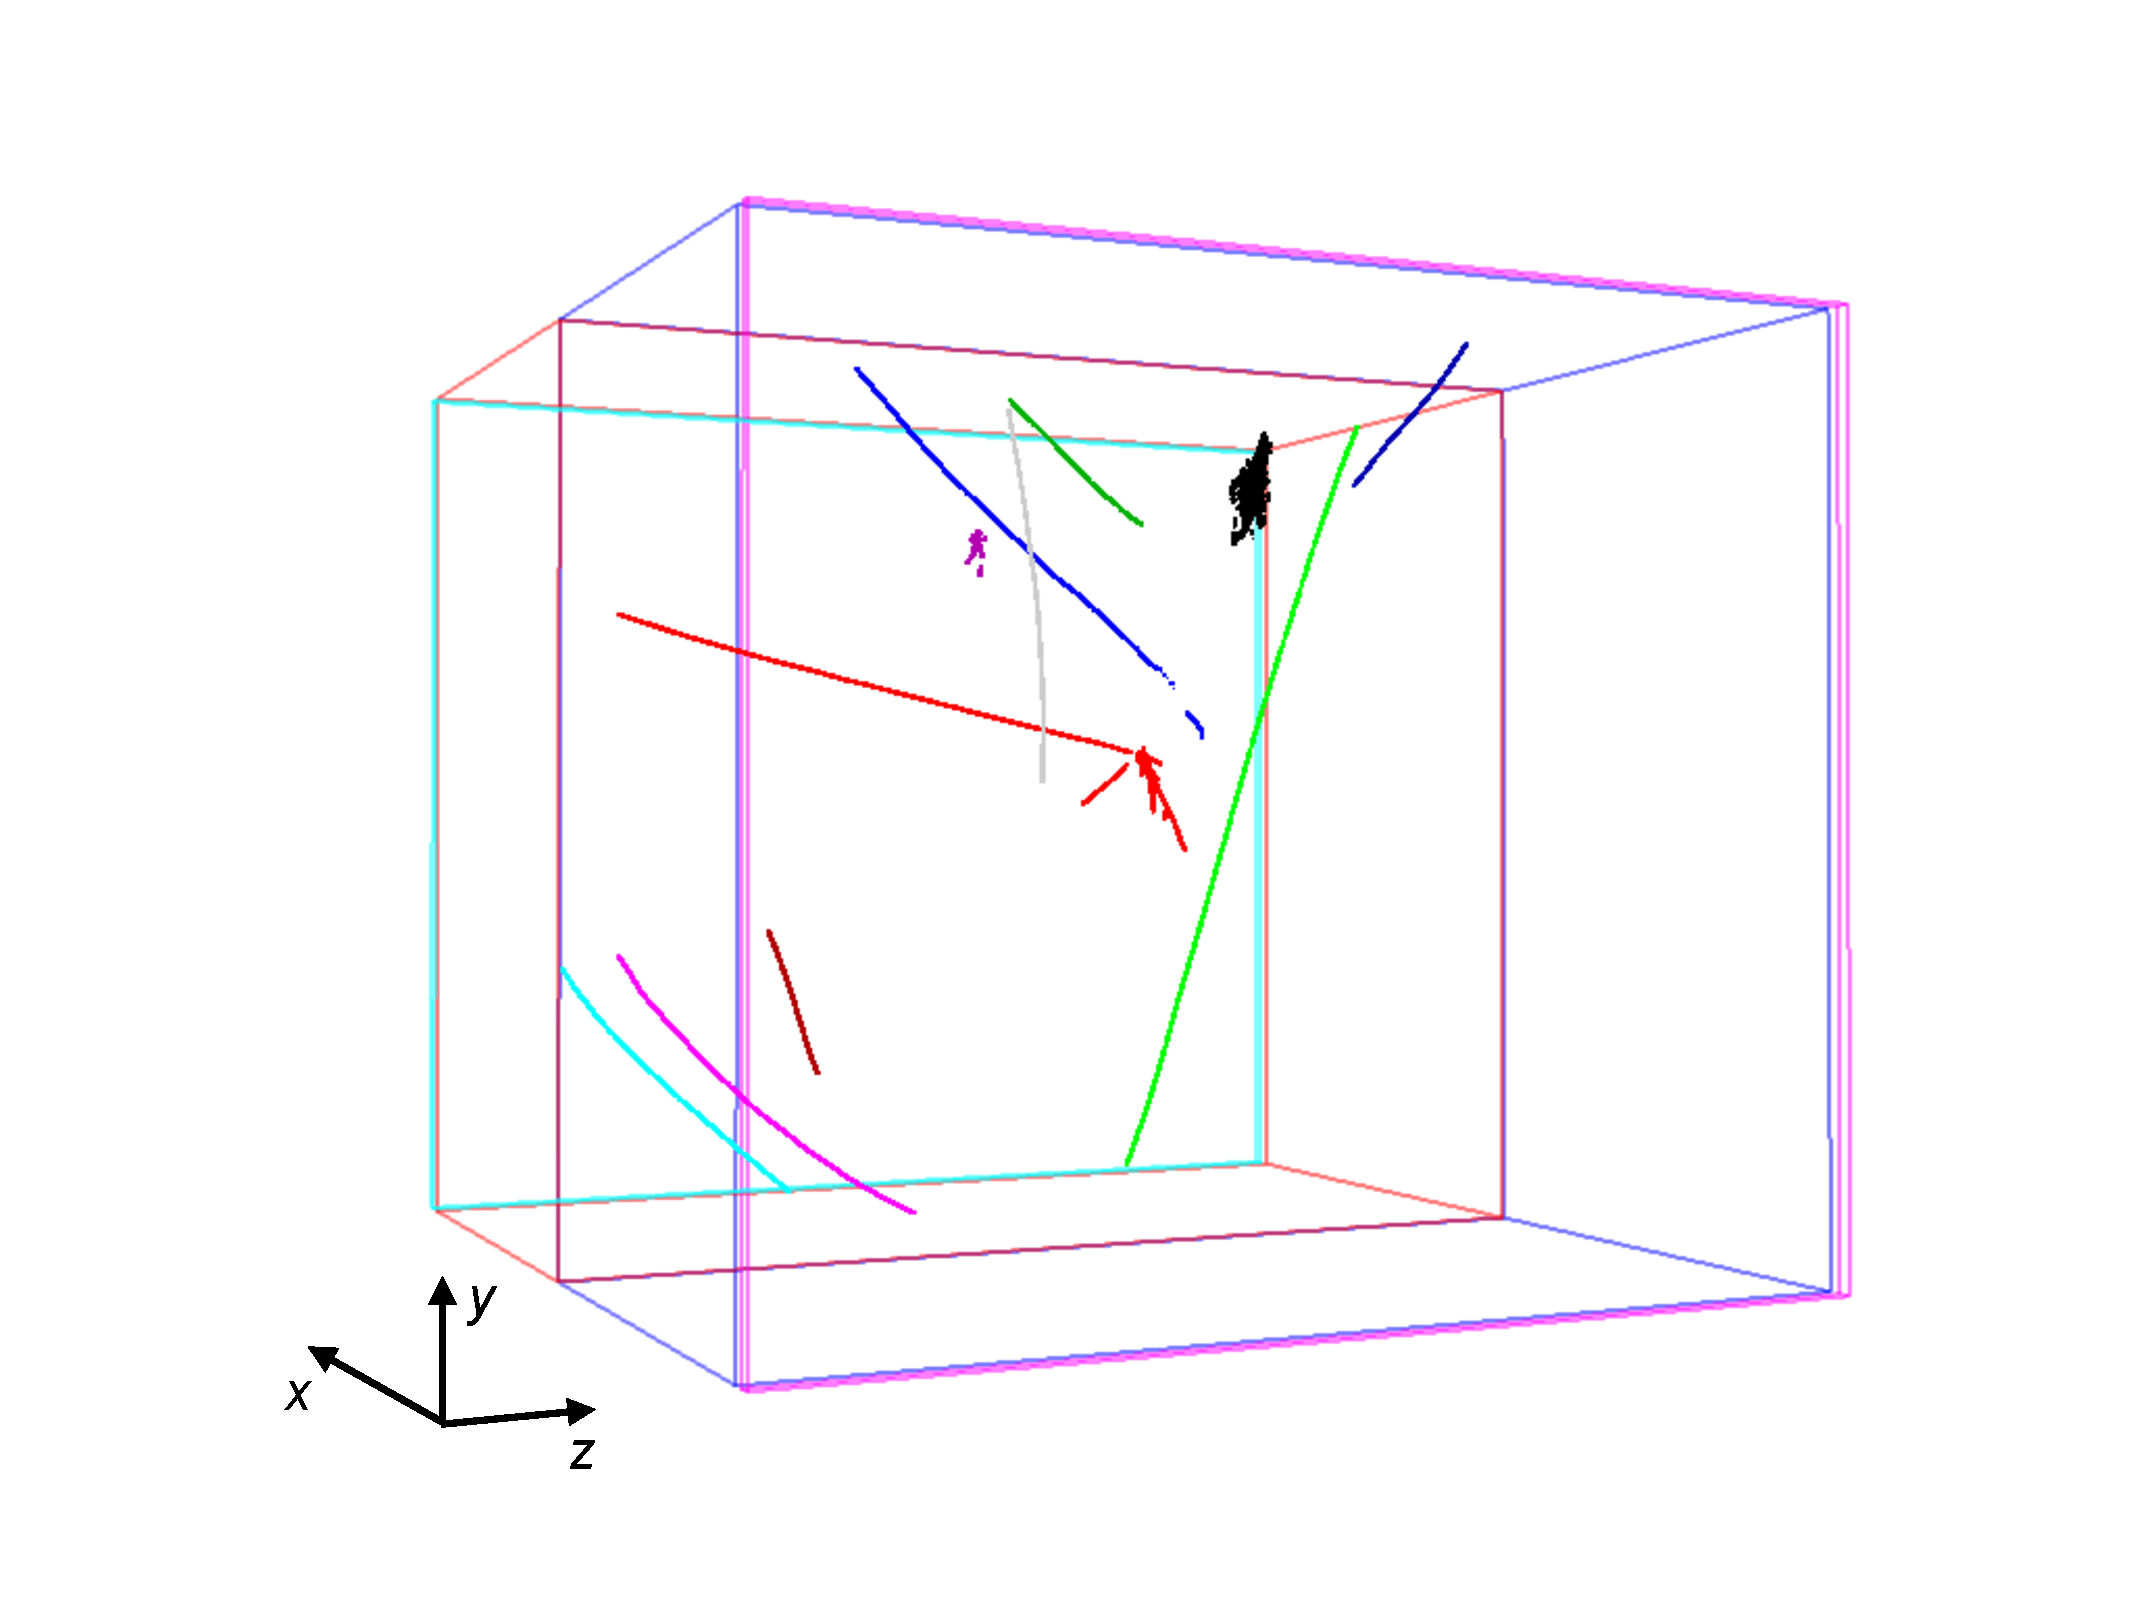
\includegraphics[width=0.6\textwidth]{Figures/Diagram/Slicing/slicing_3D_pion.pdf}\label{fig:slicing3D}} \\
\vspace{-10pt}
\subfloat[]{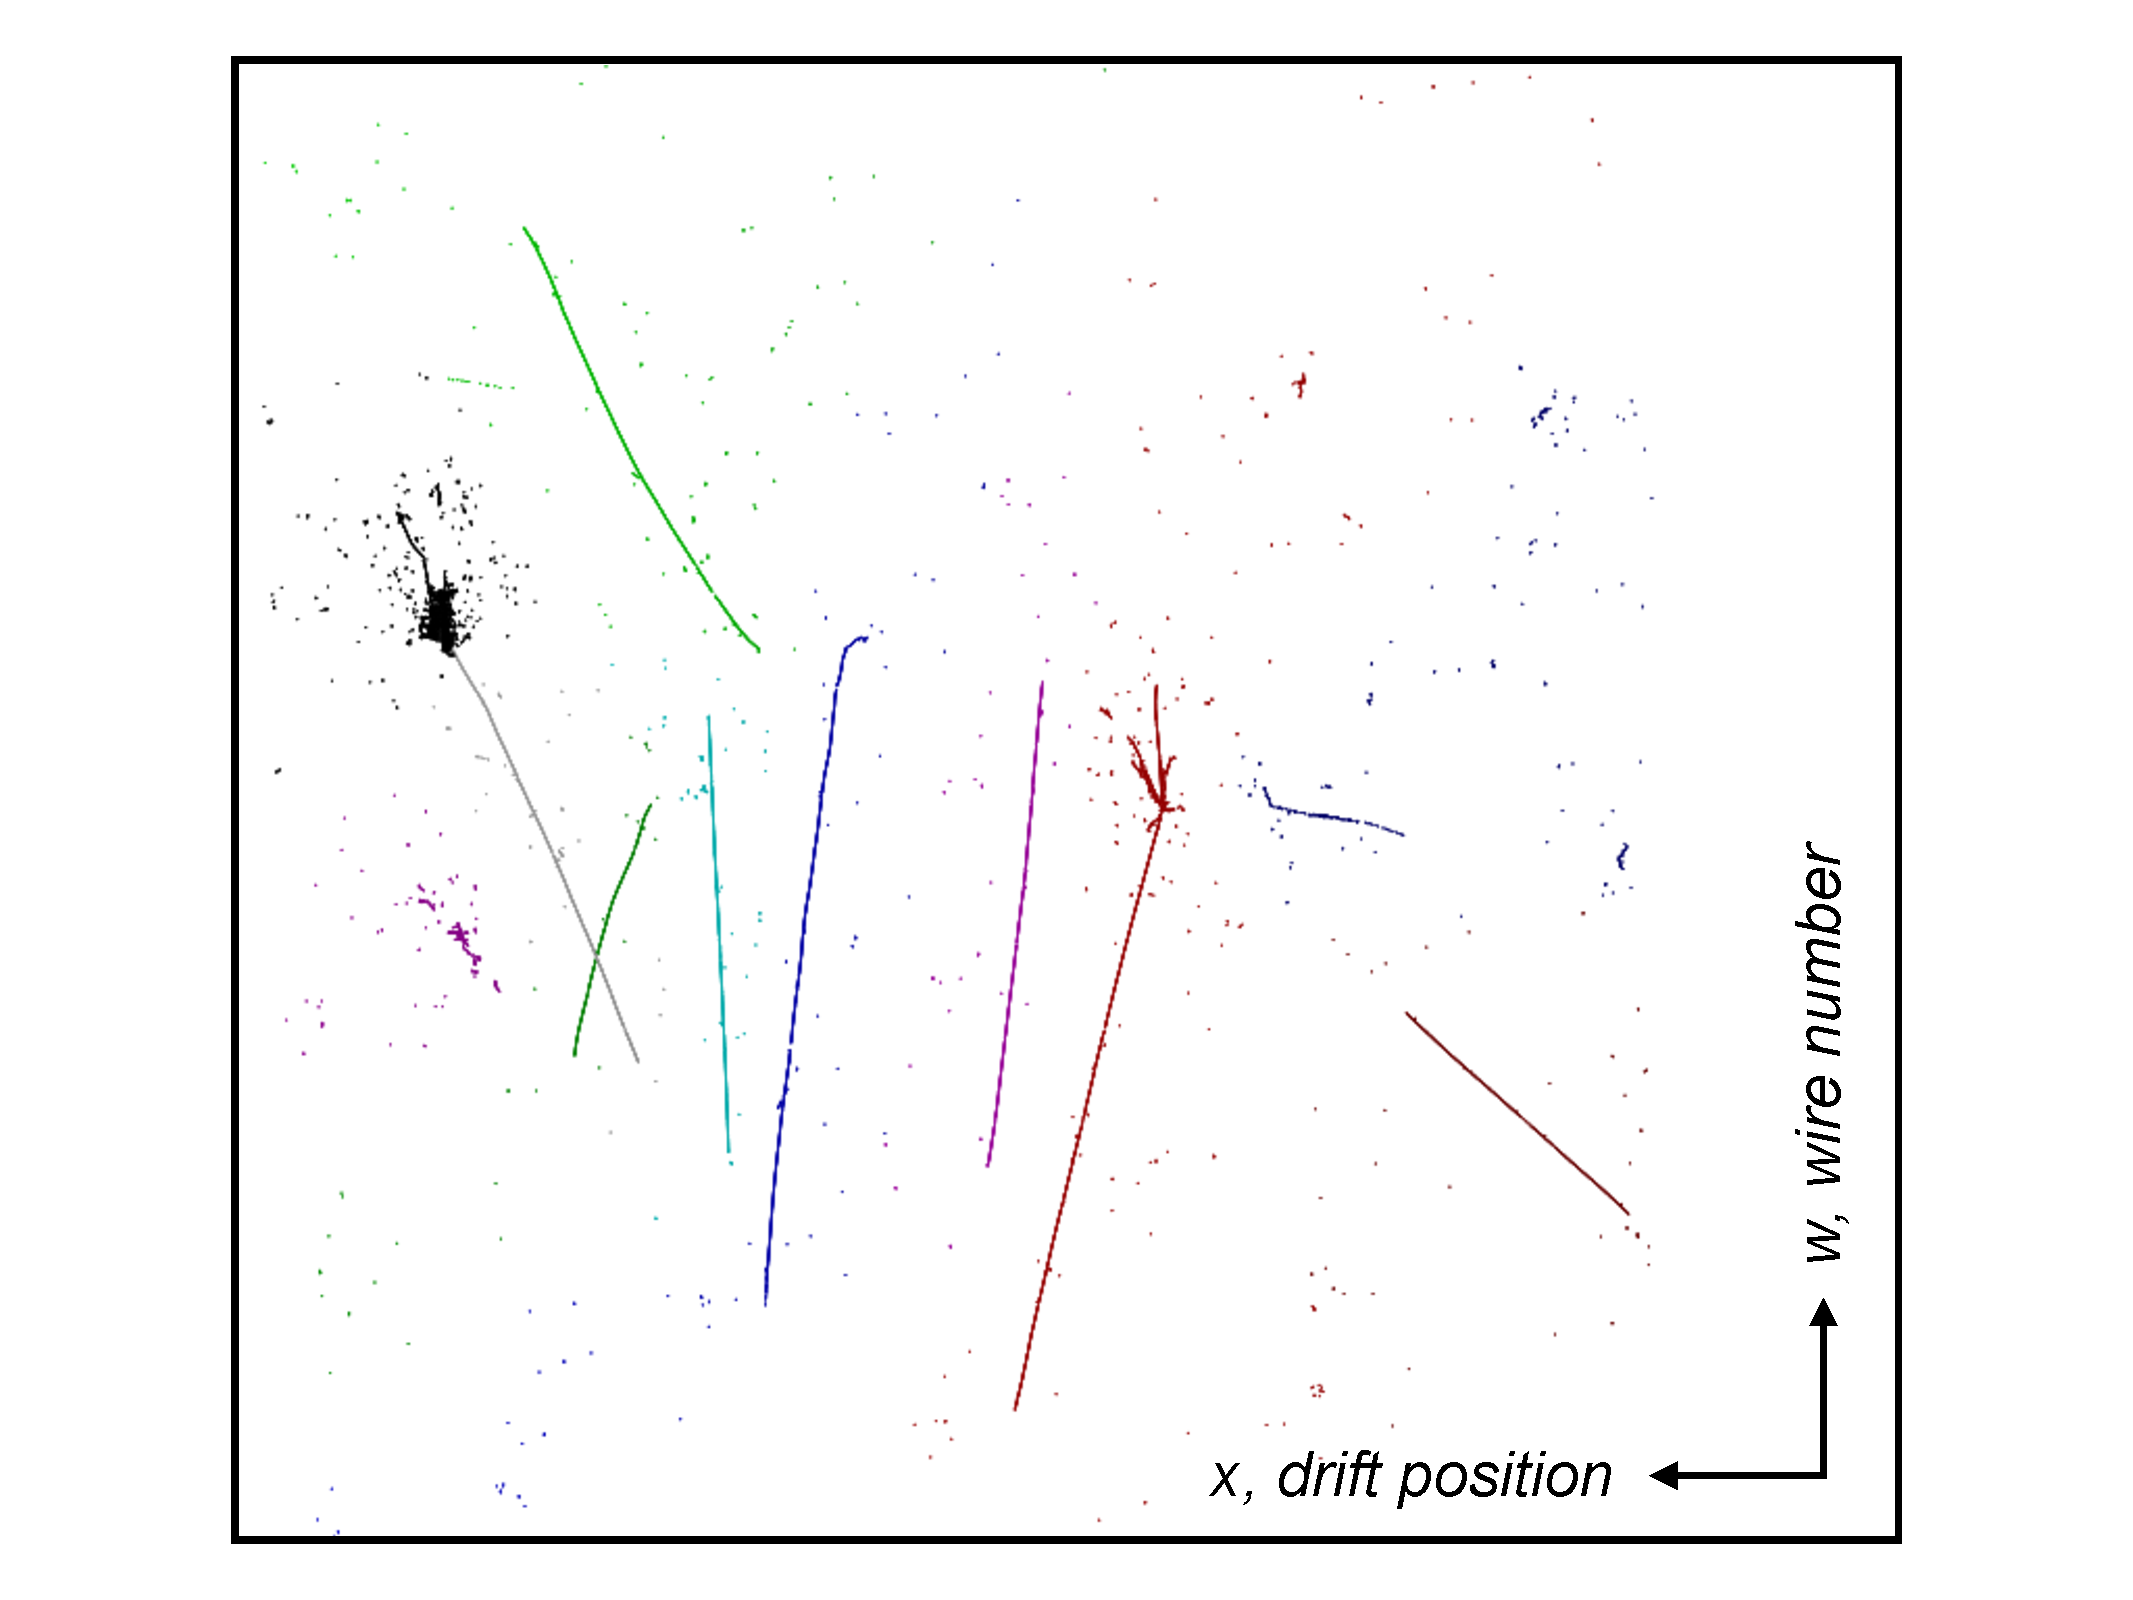
\includegraphics[width=0.33\textwidth,trim={3cm 0 3cm 0},clip]{Figures/Diagram/Slicing/slicing_2D_U_pion.pdf}\label{fig:slicingU}}
\subfloat[]{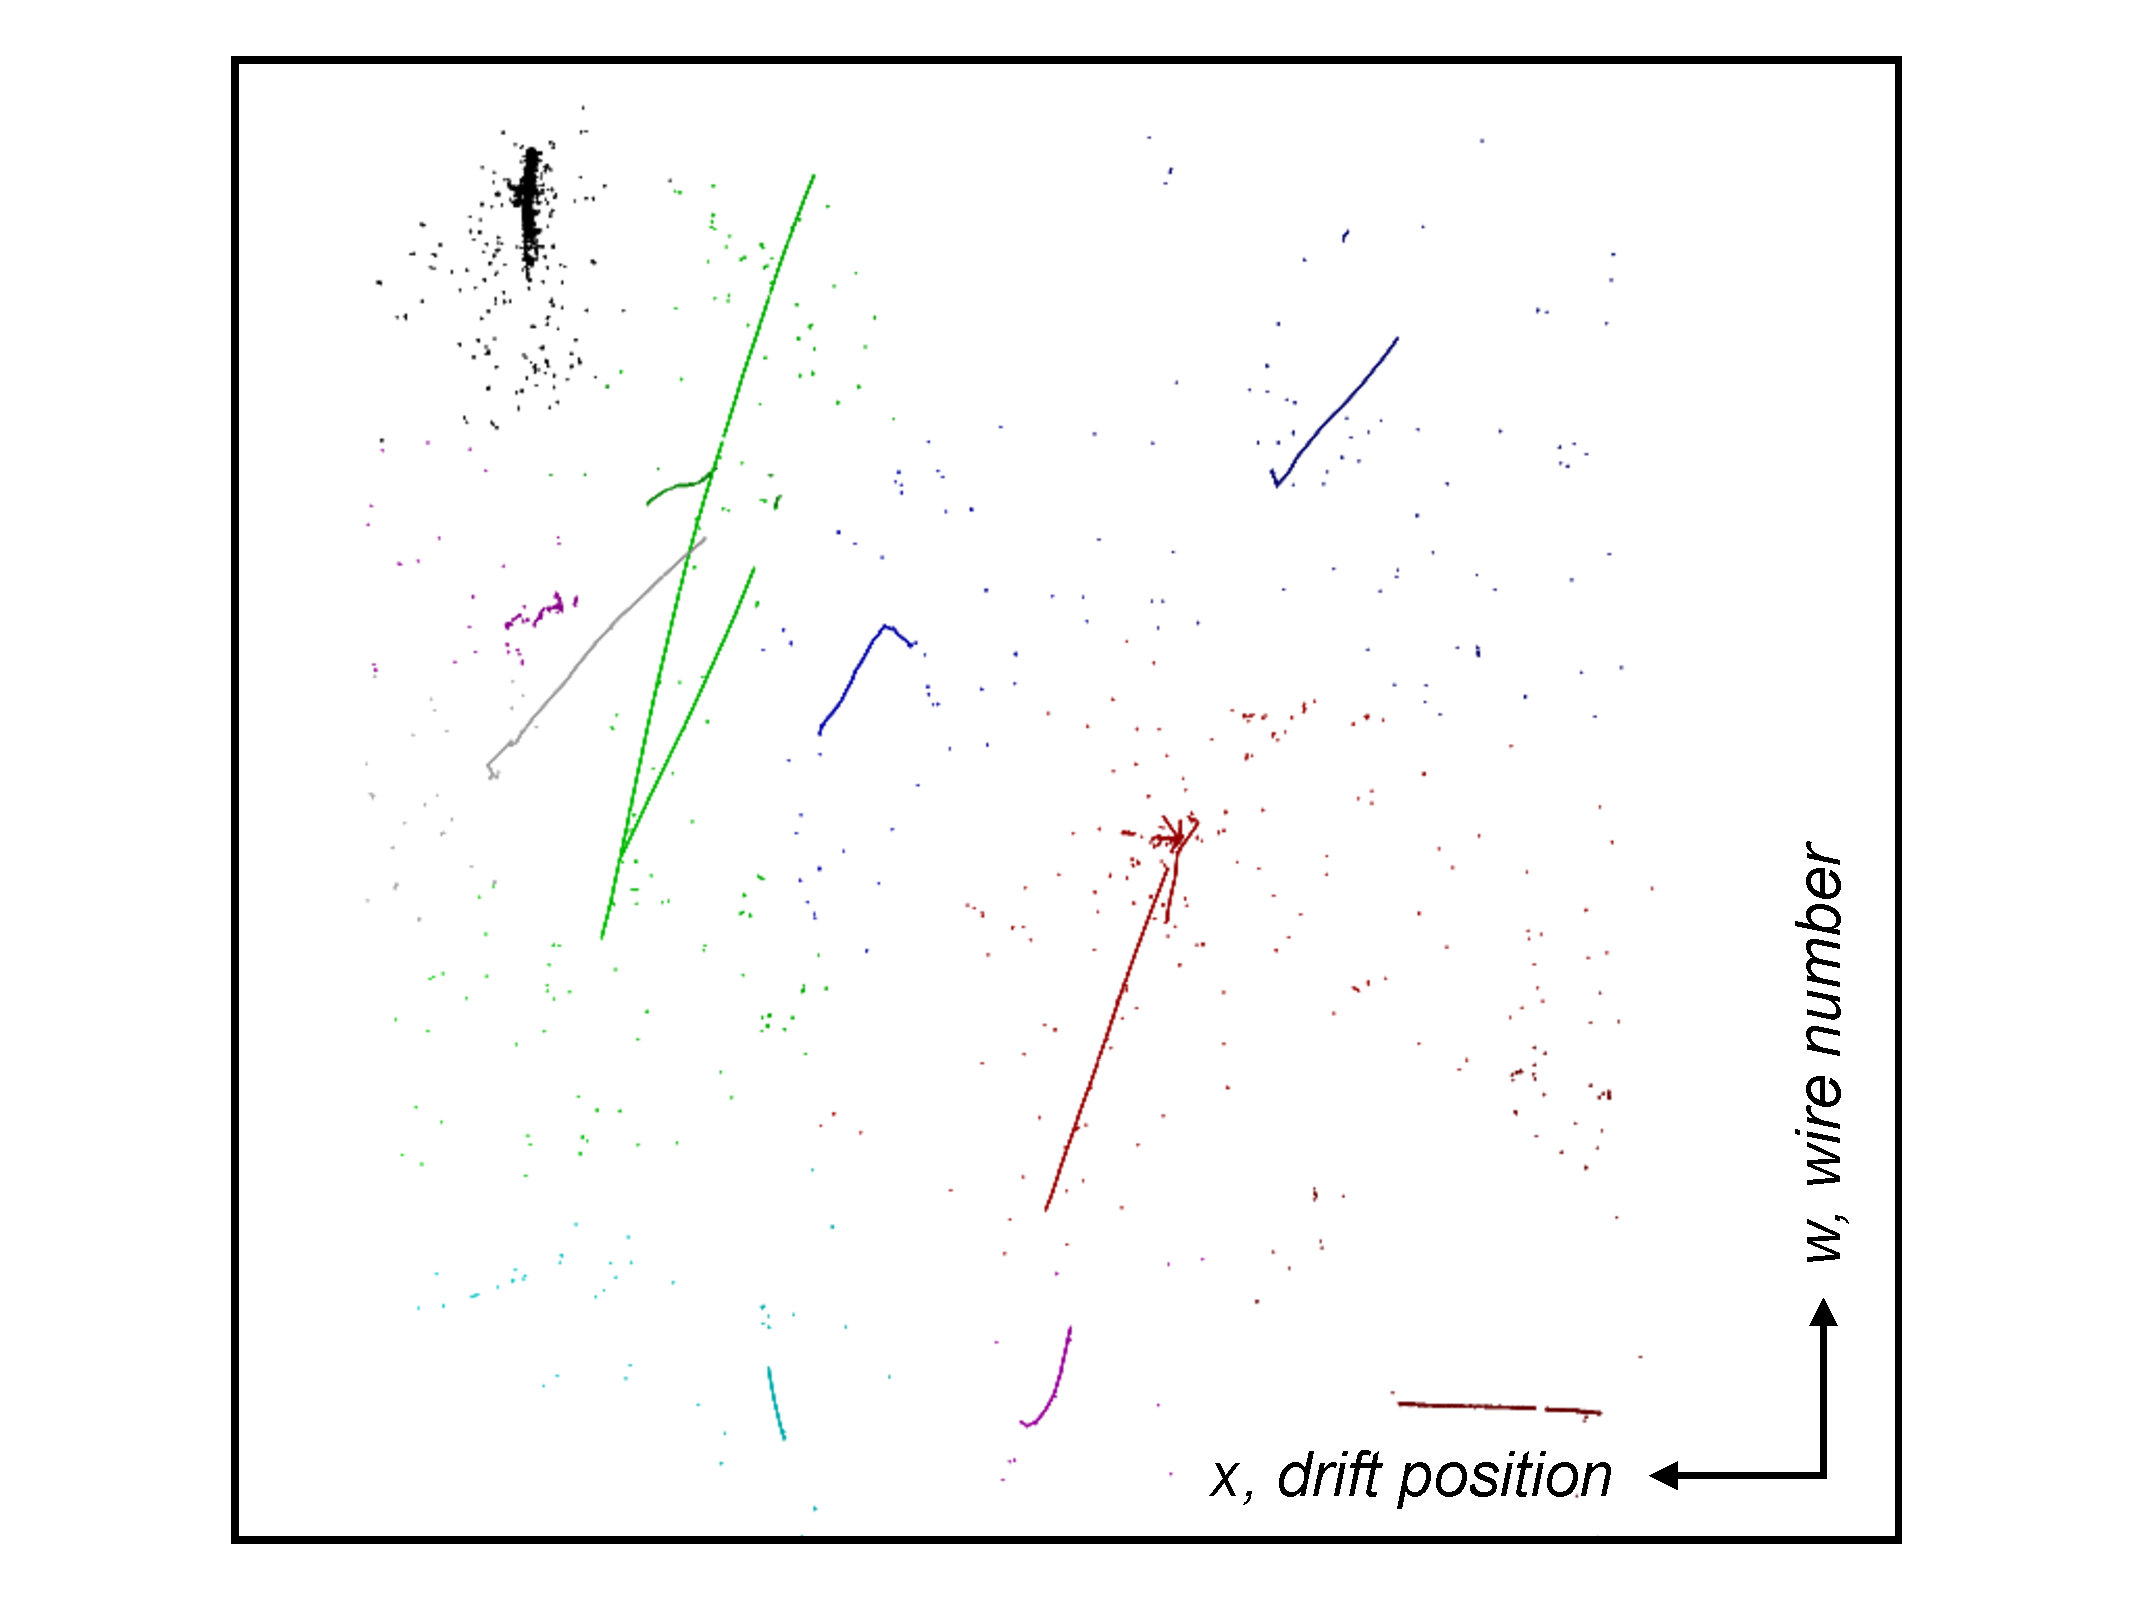
\includegraphics[width=0.33\textwidth,trim={3cm 0 3cm 0},clip]{Figures/Diagram/Slicing/slicing_2D_V_pion.pdf}\label{fig:slicingV}}
\subfloat[]{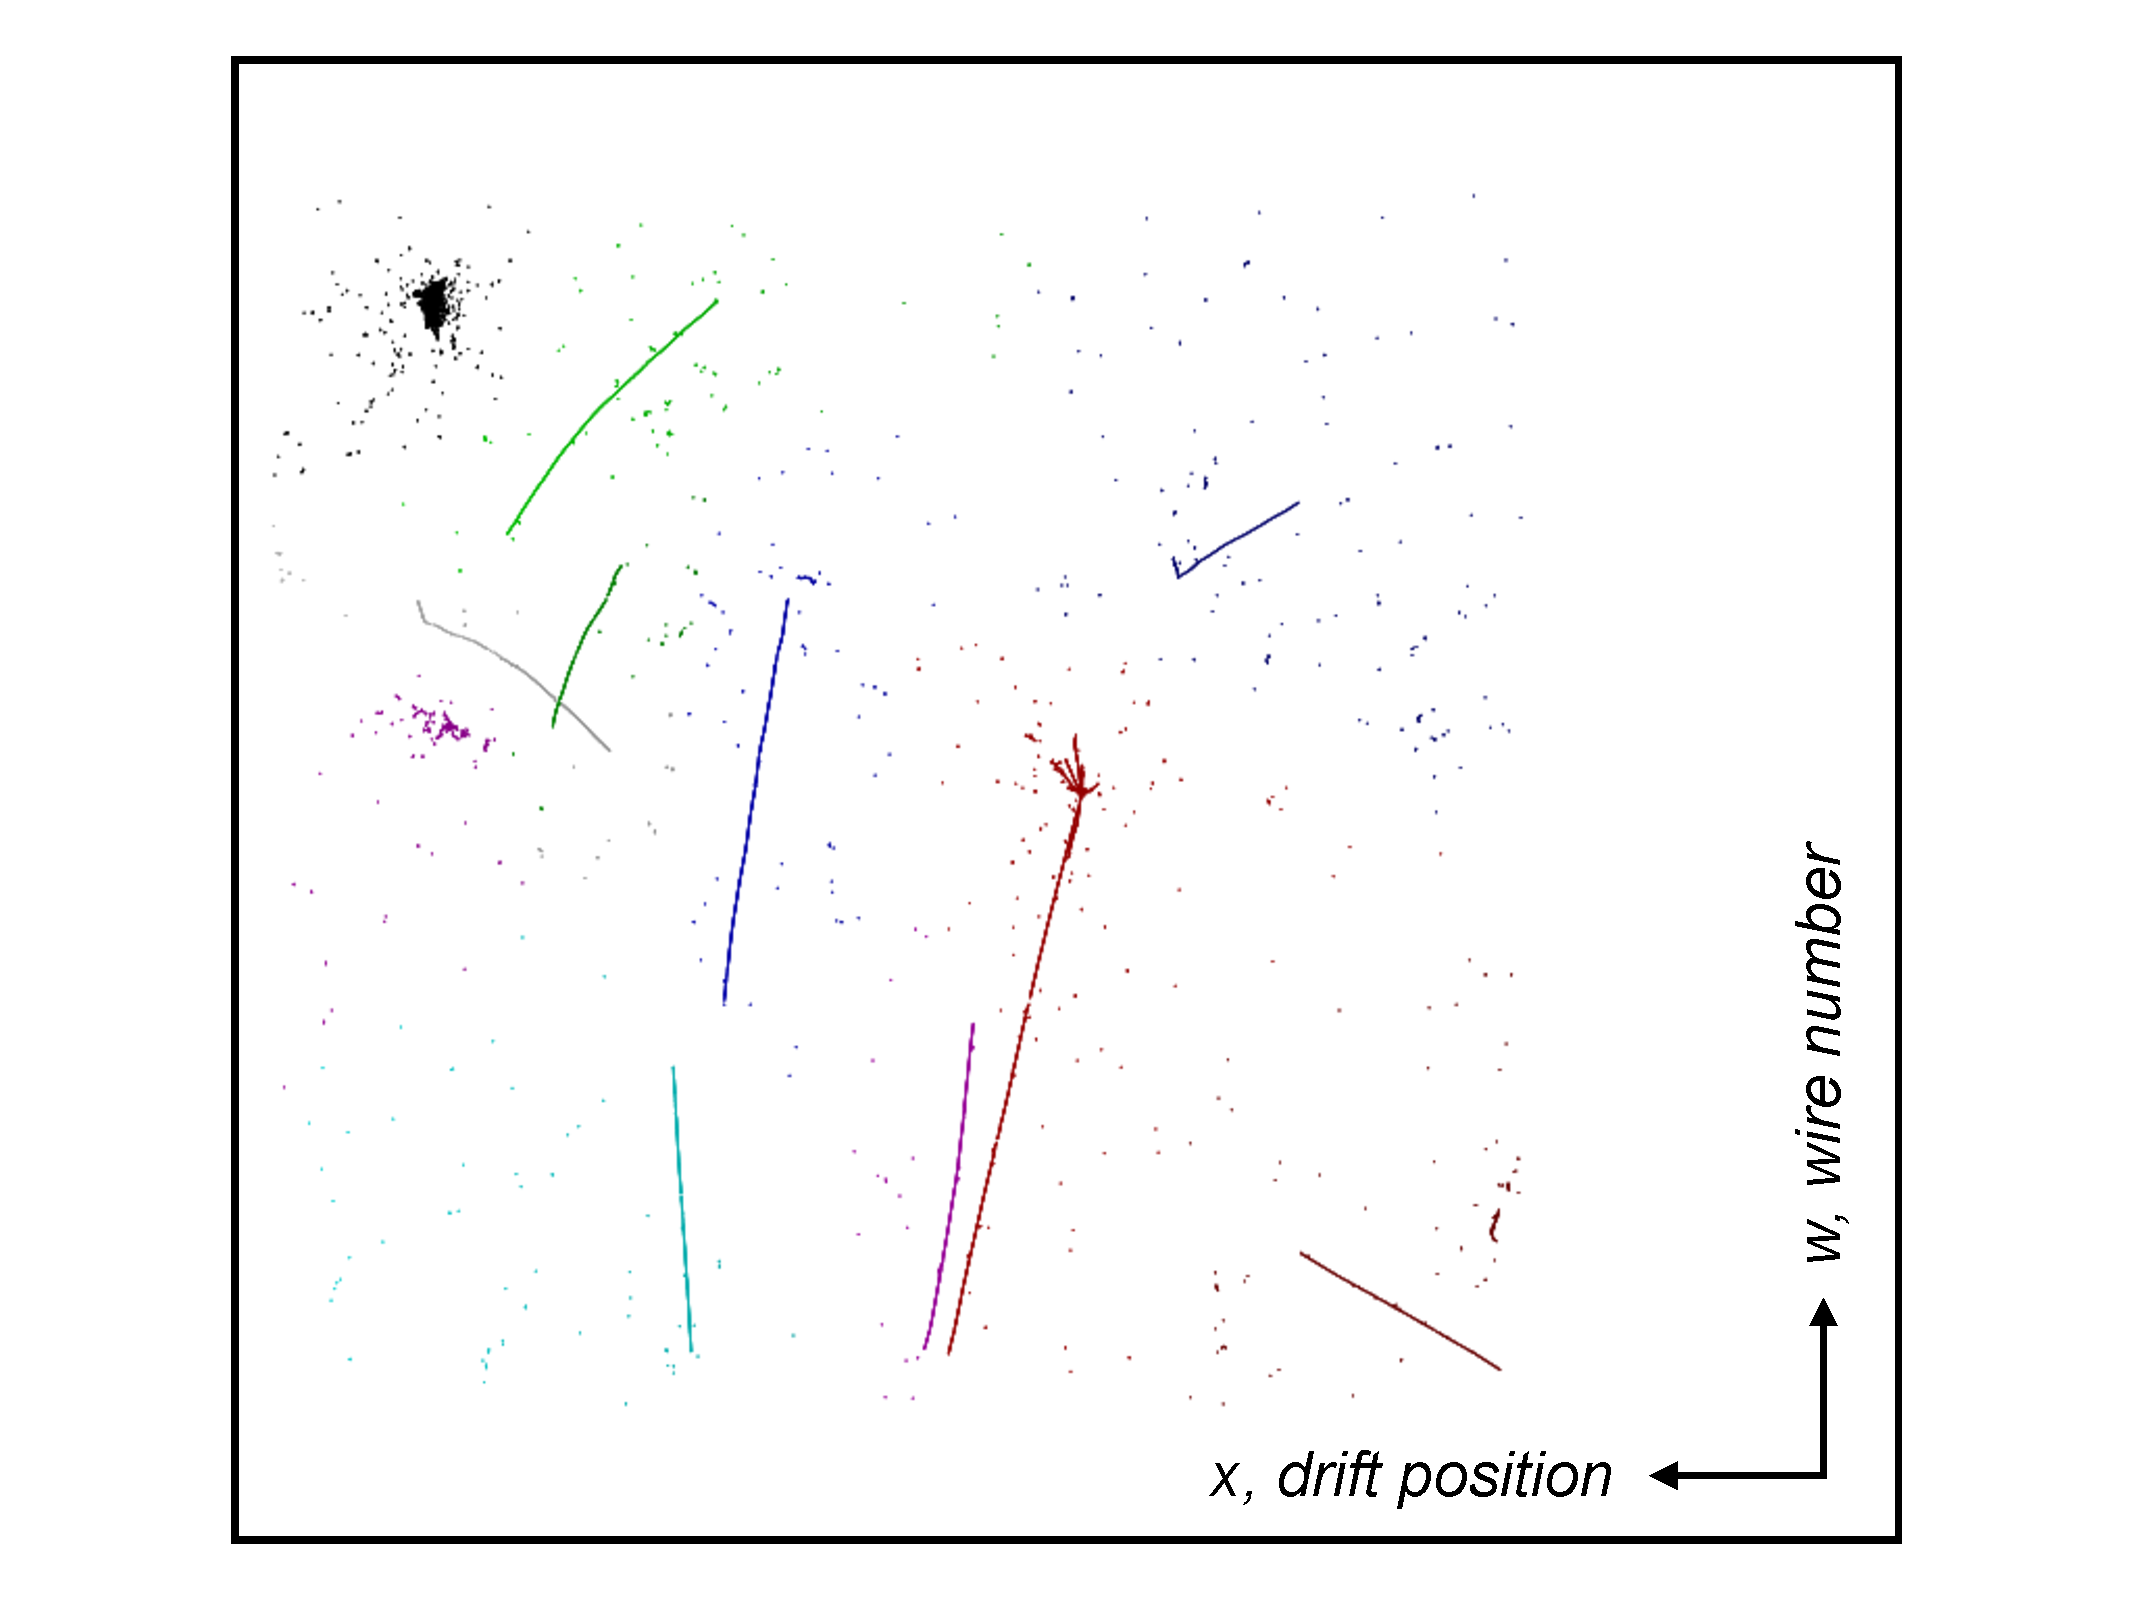
\includegraphics[width=0.33\textwidth,trim={3cm 0 3cm 0},clip]{Figures/Diagram/Slicing/slicing_2D_W_pion.pdf}\label{fig:slicingW}}
\caption{The eleven ``slices'' created during the reconstruction of a simulated 3\,GeV/$c$ $\pi^+$ ProtoDUNE-SP interaction after the removal of the clear cosmic rays. Figure~\protect\subref{fig:slicing3D} shows the 3D hits created by the `fast reconstruction' used within the slicing process, while figures \protect\subref{fig:slicingU}, \protect\subref{fig:slicingV} and \protect\subref{fig:slicingW} show the 2D hits in the $u$, $v$ and $w$ views respectively. Each unique colour represents a distinct slice, and the reconstructed beam particle slice is shown in red.}
\label{fig:slicing}
\end{figure*}

%The Pandora slicing worker instance 
In order to perform the slicing in 3D, a subset of algorithms based on the PandoraTestBeam chain are run, but (for speed) the finesse of vertex identification and building particle hierarchies is neglected. All that is required is that groups of hits are associated in 3D, and separated from groups originating from different primary particles. By applying this fast reconstruction, correlations across the three input views are considered when dividing up the event into separate slices. This approach is more powerful than dividing up each view independently. An example of the slicing procedure is shown in Fig.~\ref{fig:slicing}. The output of the slicing algorithm is a list of hits produced for each reconstructed slice, and all hits that were input to the slicing algorithm must be assigned to a slice. In the remaining reconstruction stages the slices are processed separately.

\subsubsection{Slice Identification}

After the event slicing, different reconstruction hypotheses can be applied to each slice. The idea is that, for each individual slice, the hypothesis that produces the most appropriate (``best'') reconstruction outcome can be selected. Each slice will have exactly one outcome selected, and the consolidated event will be built from: i) the clear cosmic-ray muon hierarchies and ii) one selected outcome for each slice. The two hypotheses tested for ProtoDUNE-SP are the PandoraTestBeam and PandoraCosmic chains. Each slice is therefore reconstructed independently by the PandoraCosmic and PandoraTestBeam algorithm chains, providing two possible reconstruction outcomes.

The next step is to select exactly one of the two different reconstruction outcomes for each slice and in ProtoDUNE-SP this decision is made using a BDT. The following features are calculated for the two different slice outcomes, and both sets are used as inputs to the BDT:

\begin{itemize}
\item The number of reconstructed particles in the slice.
\item The distance between the point at which the test beam is expected to enter the detector and the closest 3D hit.
\item The vertical distance between the top face of the detector and the closest reconstructed 3D hit.
\item The eigenvalues of the covariance matrix from a principal component analysis of the reconstructed 3D hits.
\item The opening angle between the principal axis of the reconstructed 3D hits and the expected direction of the test beam.
\end{itemize}

These features are motivated by the fact that the entrance position and direction of the test beam is well understood. Cosmic-ray muons typically enter through the top face of the detector and produce highly track-like topologies in the detector in contrast to the typically more complex test-beam particle interactions.

A threshold is applied to the output score from the BDT and those slices with scores exceeding the threshold are classified as test-beam particles, while all remaining slices are classified as cosmic-ray muons. The PandoraTestBeam reconstruction outcome is selected for all slices classified as test-beam particles, while the PandoraCosmic reconstruction is chosen for all slices classified as cosmic-ray muons.

Figure~\ref{fig:examplemcreco} shows the reconstruction output for a candidate 1\,GeV/$c$ $\pi^{+}$ charge exchange event in ProtoDUNE-SP data, where the test-beam particle has been correctly distinguished from the cosmic-ray muon background. The zoomed view shows that the parent $\pi^{+}$ beam particle has been identified (purple, moving from left to right) and correctly placed at the top of the reconstructed hierarchy, and two $\pi^0$ decay photons emanating from the primary interaction vertex have been reconstructed (black and red) and added to the reconstructed hierarchy as child particles. Alongside the 3D reconstructed output, this figure also shows the 2D hits that form the reconstructed particles in the $u$, $v$ and $w$ views. 

\begin{figure*}[htb]
\centering
\subfloat[]{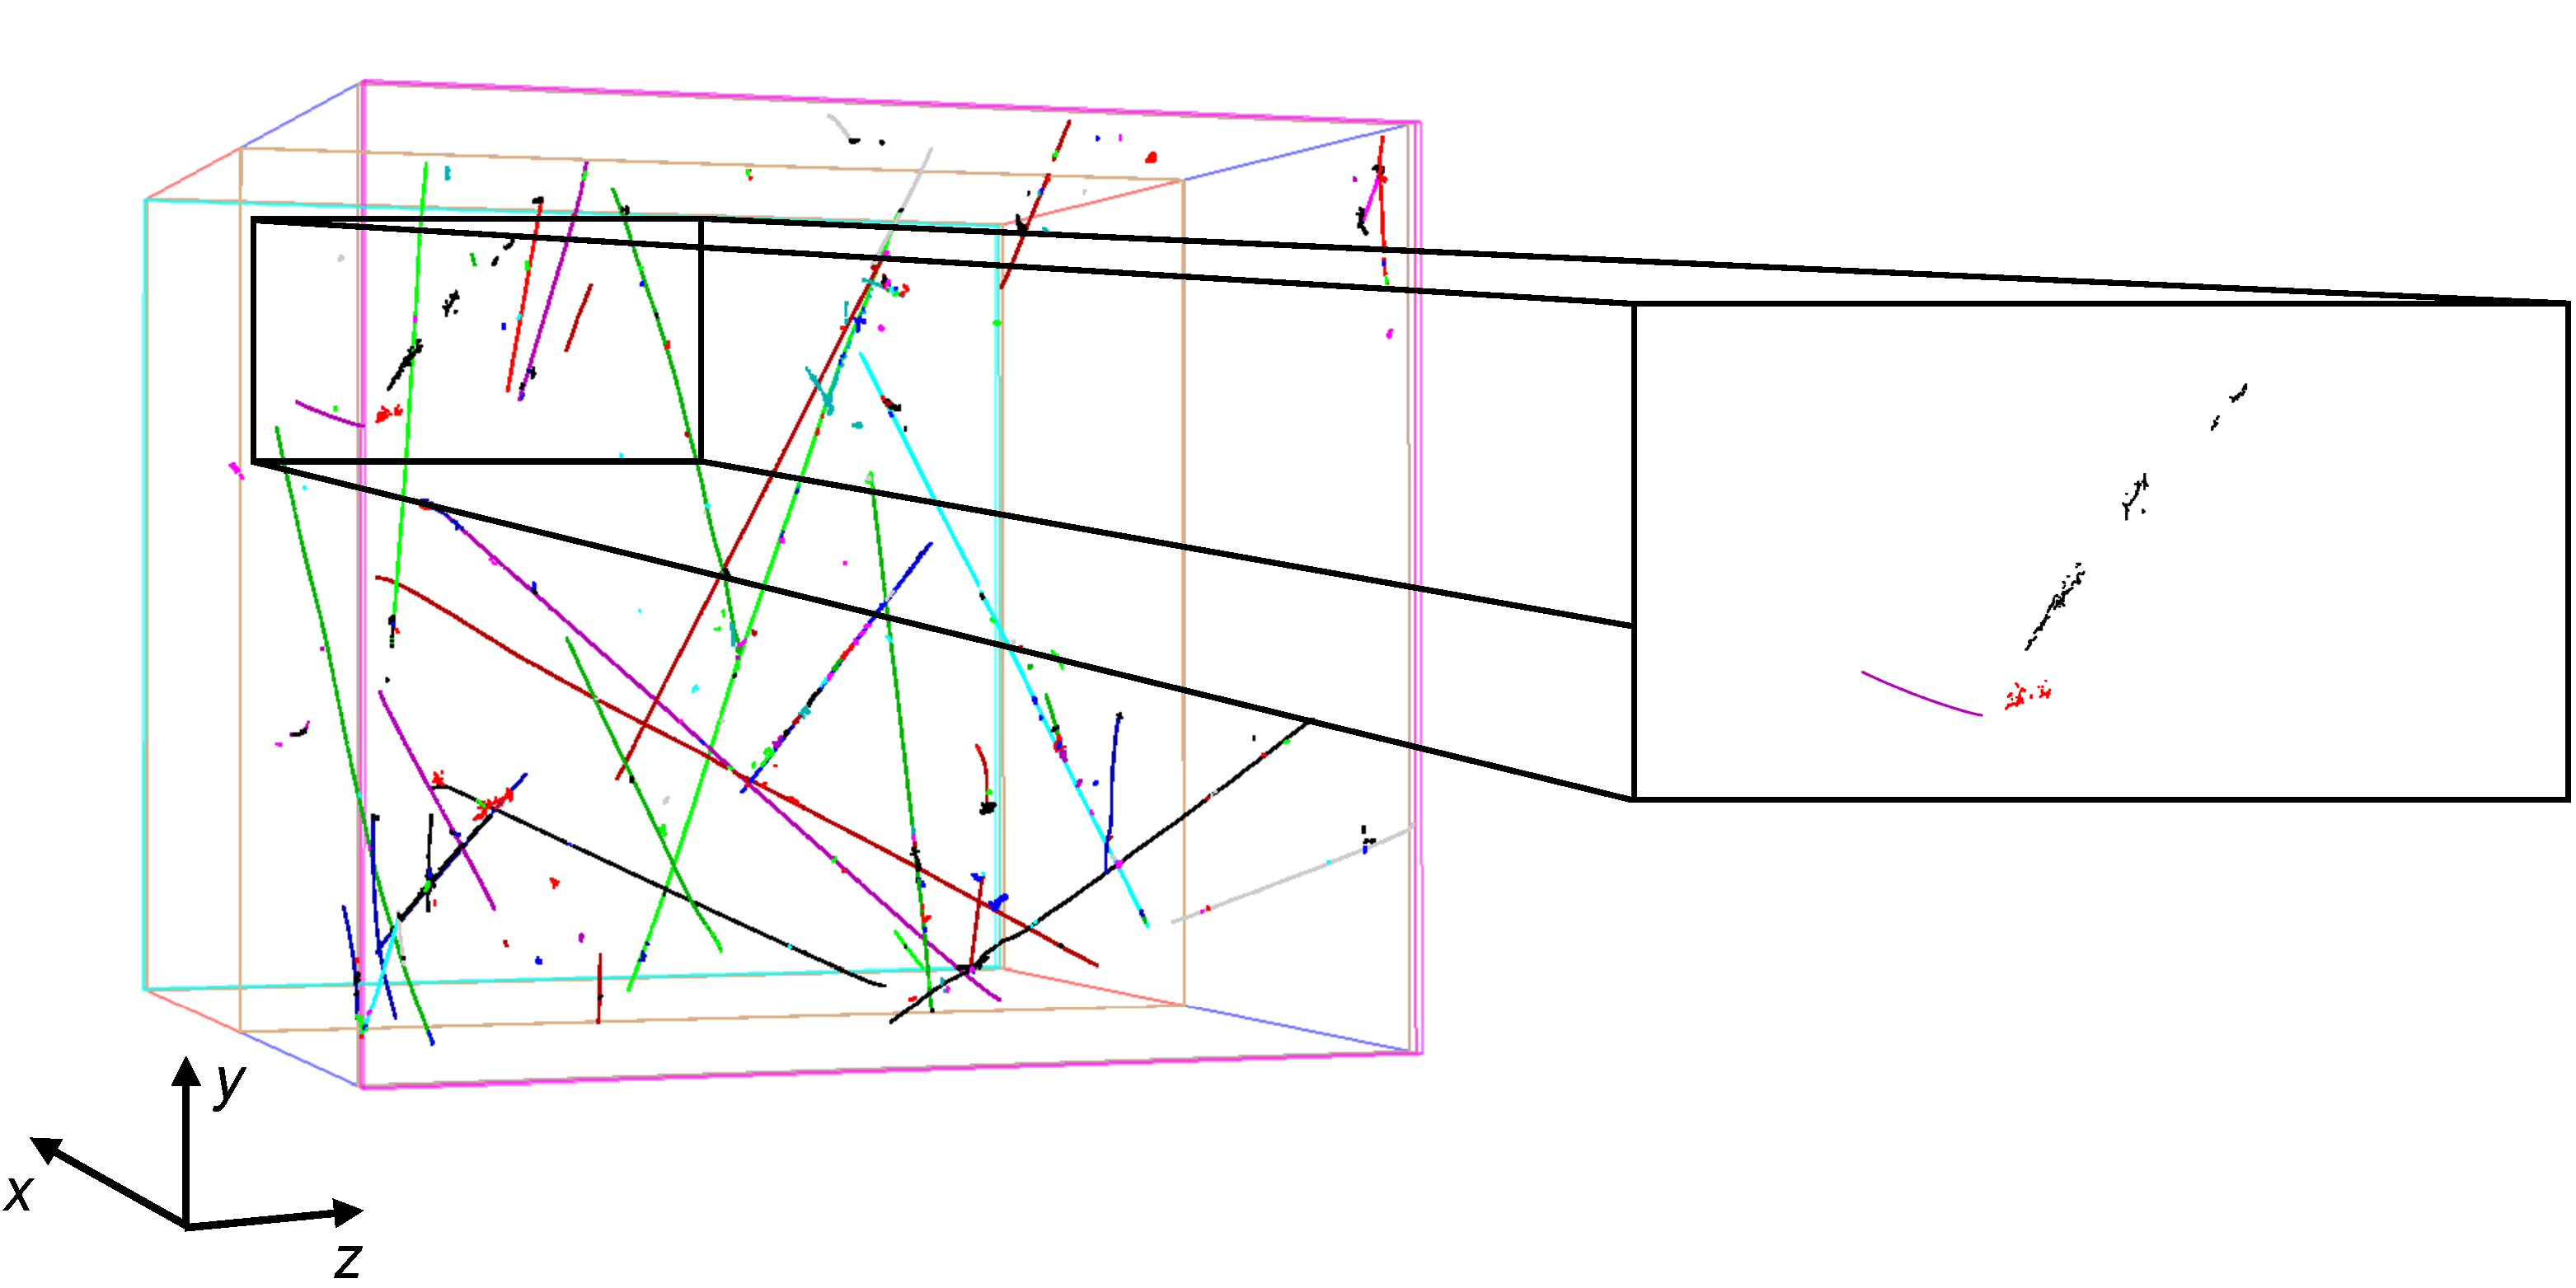
\includegraphics[width=0.9\textwidth,trim={0 0 0 0},clip]{Figures/EventDisplays/Data/full_event_3D_pion_with_zoom_data.pdf}\label{fig:examplemcrecoa}} \\
\vspace{-10pt}
\subfloat[]{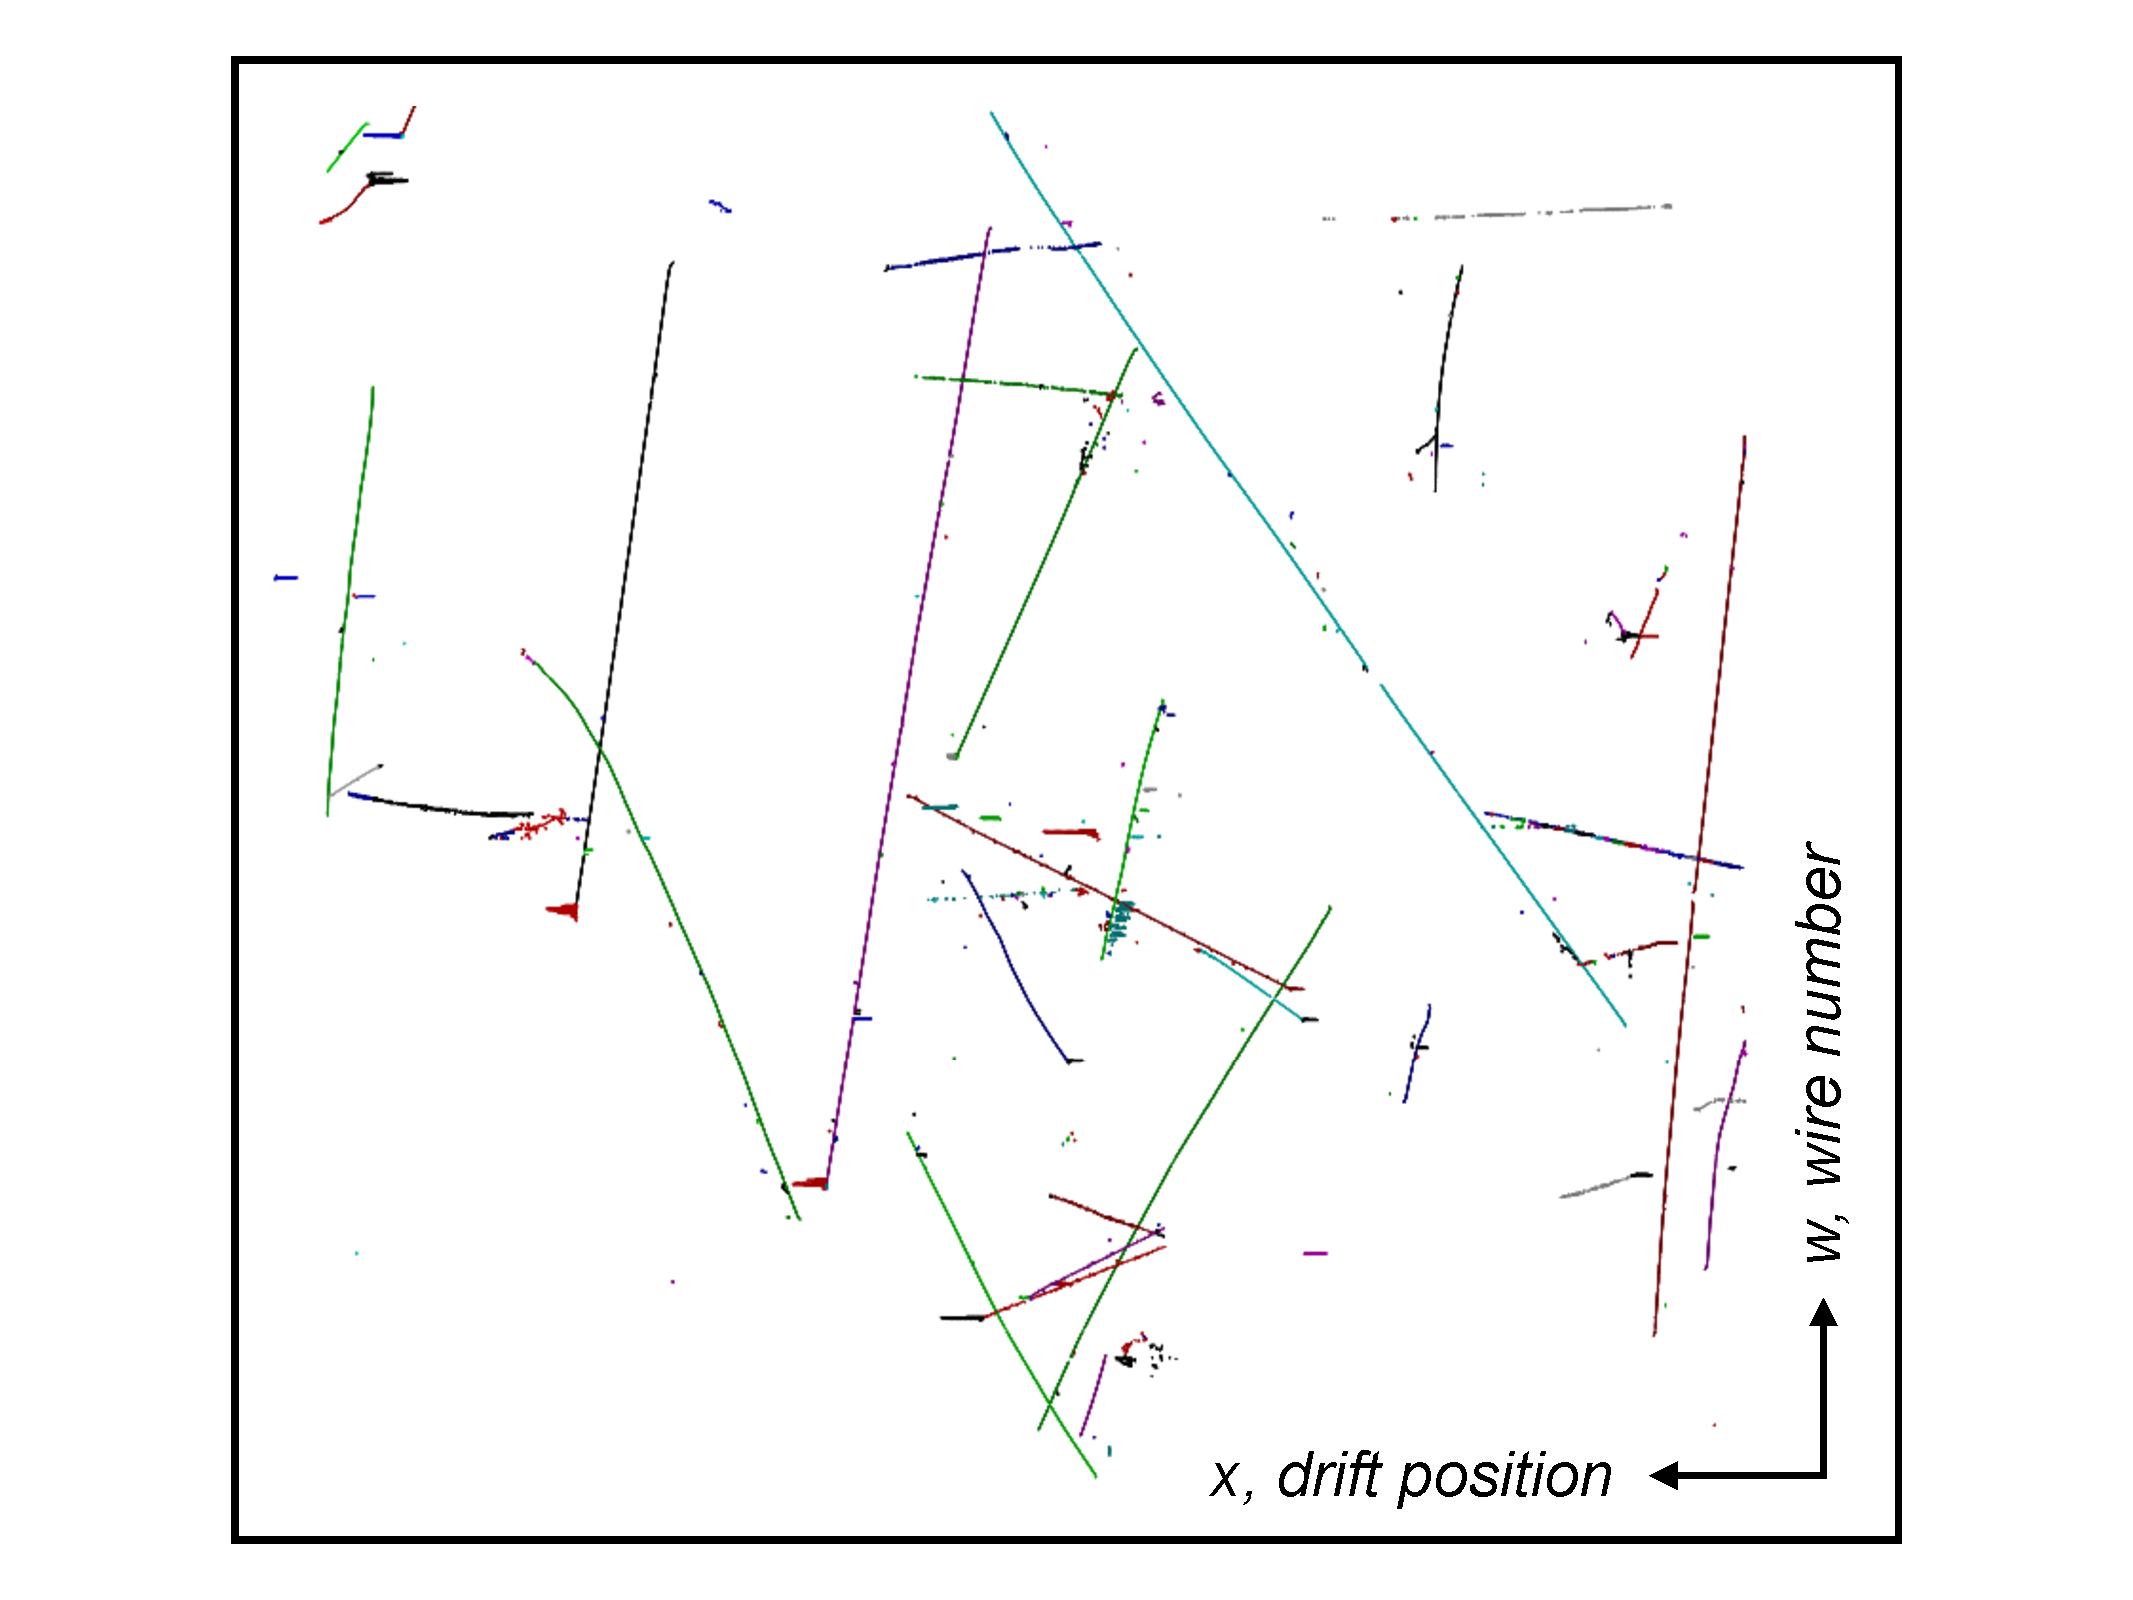
\includegraphics[width=0.33\textwidth,trim={3cm 0 3cm 0},clip]{Figures/EventDisplays/Data/full_event_2D_U_data.pdf}\label{fig:examplemcrecob}}
\subfloat[]{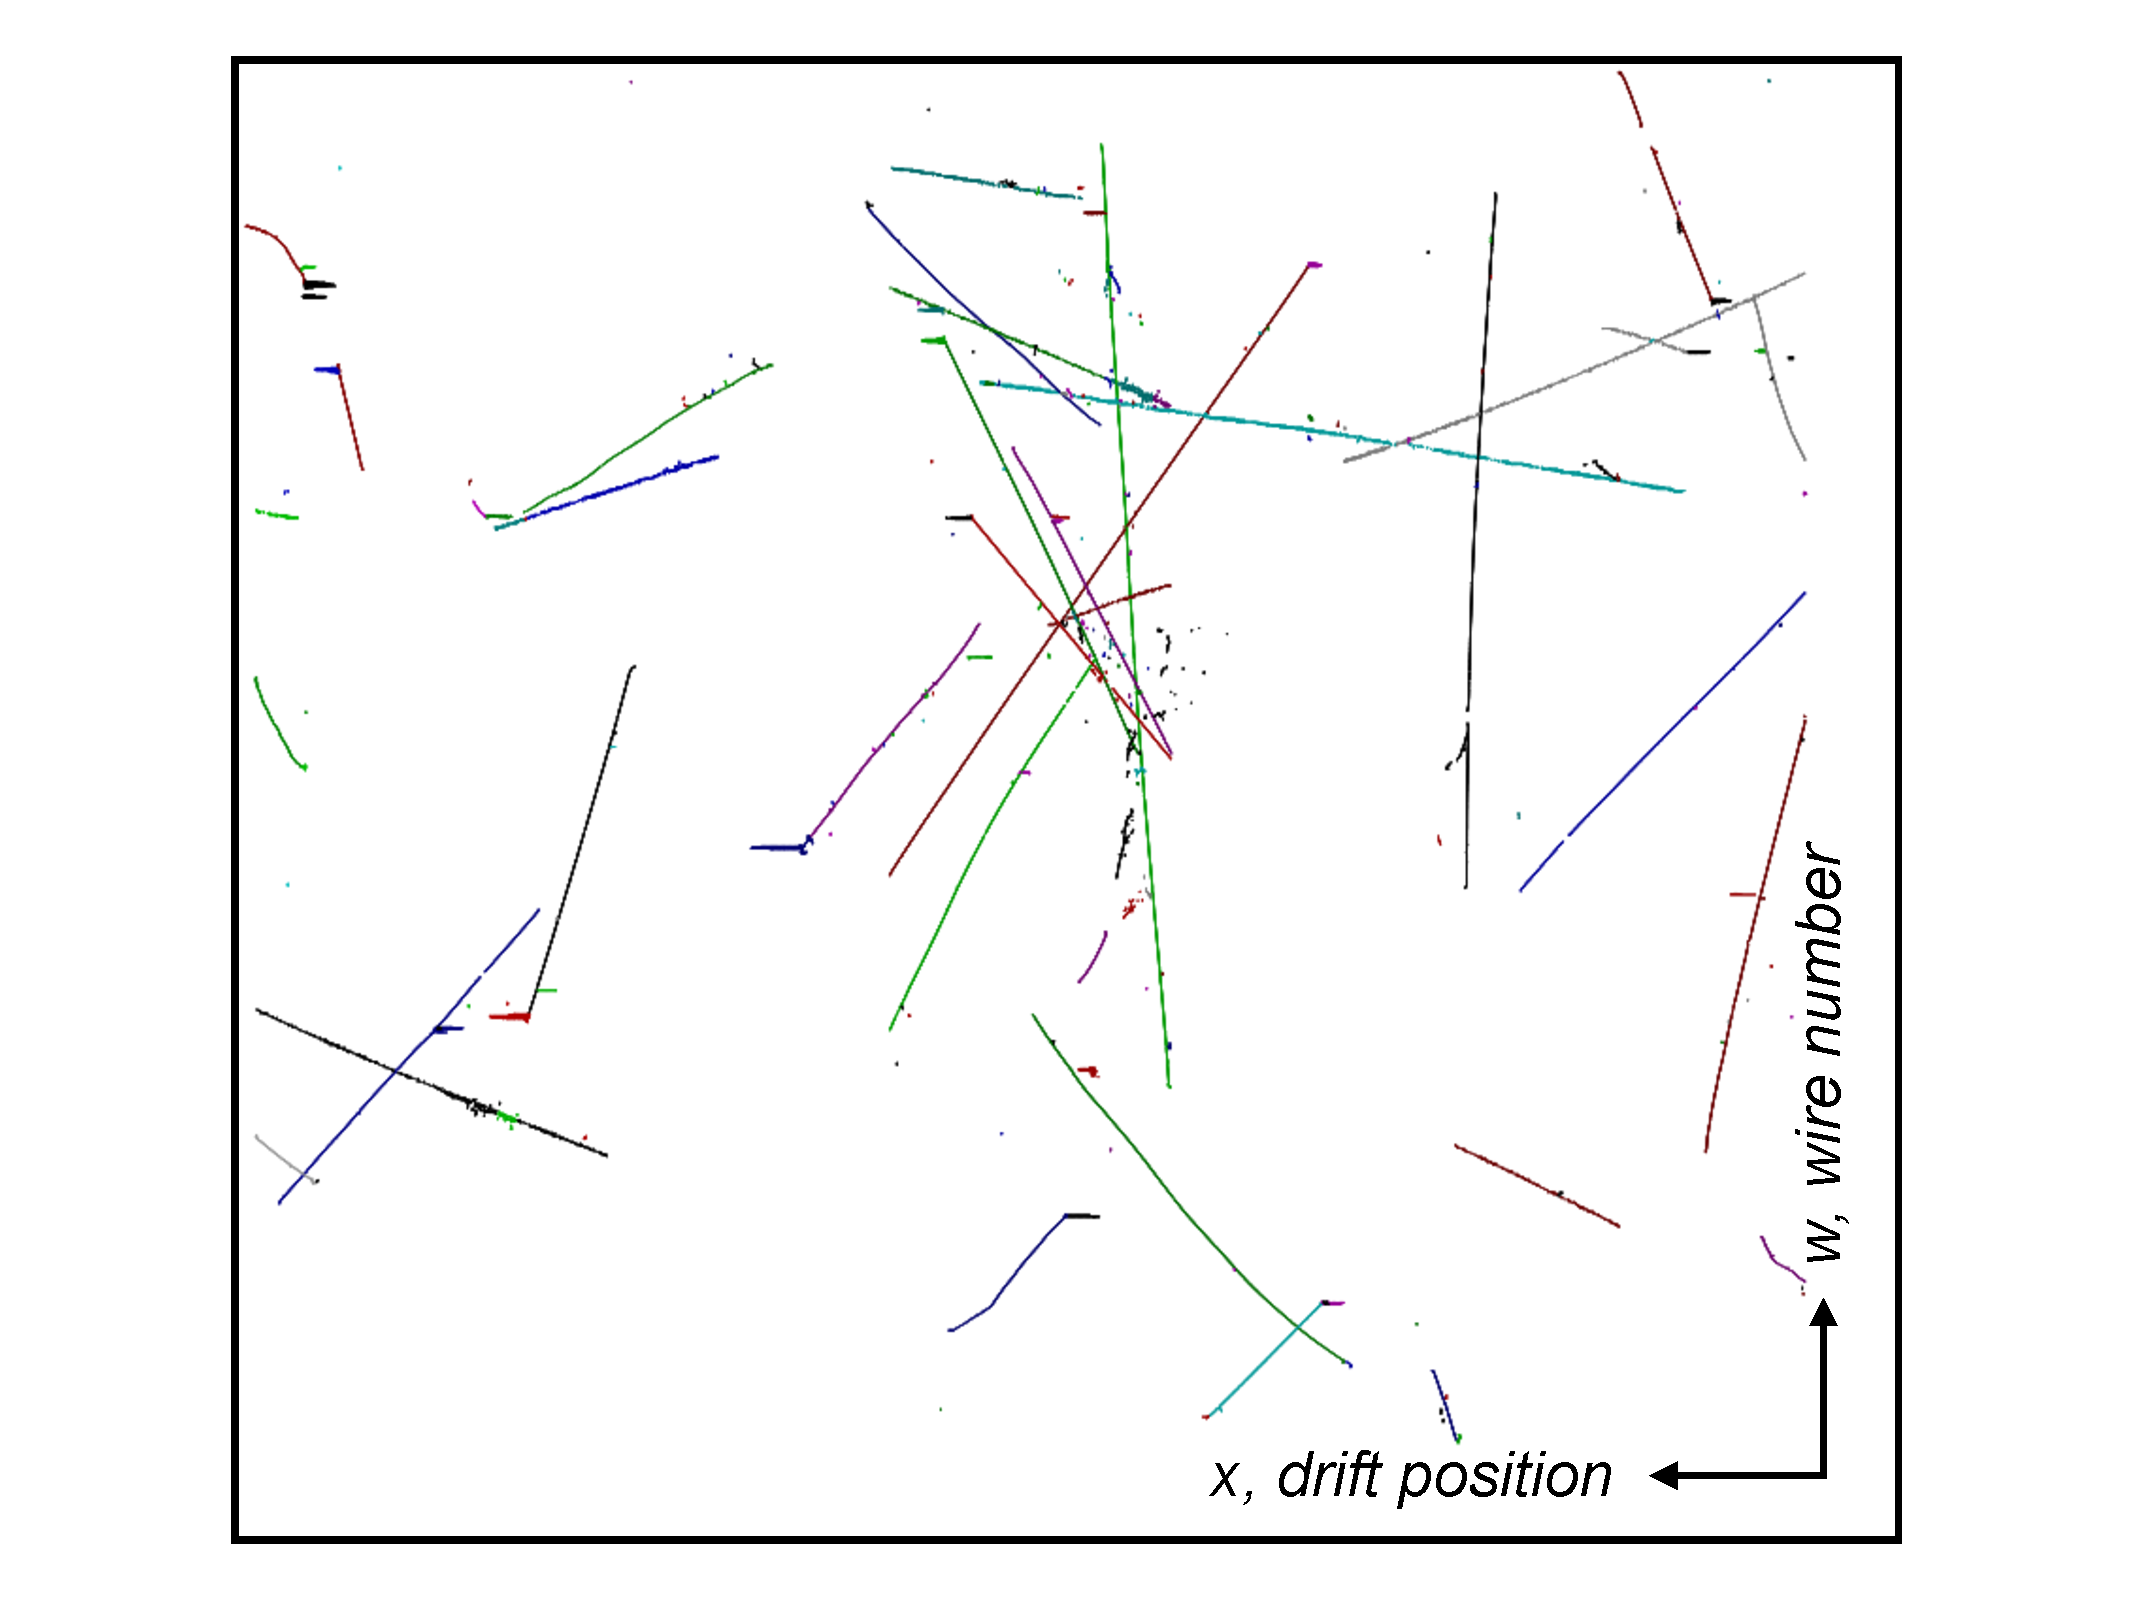
\includegraphics[width=0.33\textwidth,trim={3cm 0 3cm 0},clip]{Figures/EventDisplays/Data/full_event_2D_V_data.pdf}\label{fig:examplemcrecoc}}
\subfloat[]{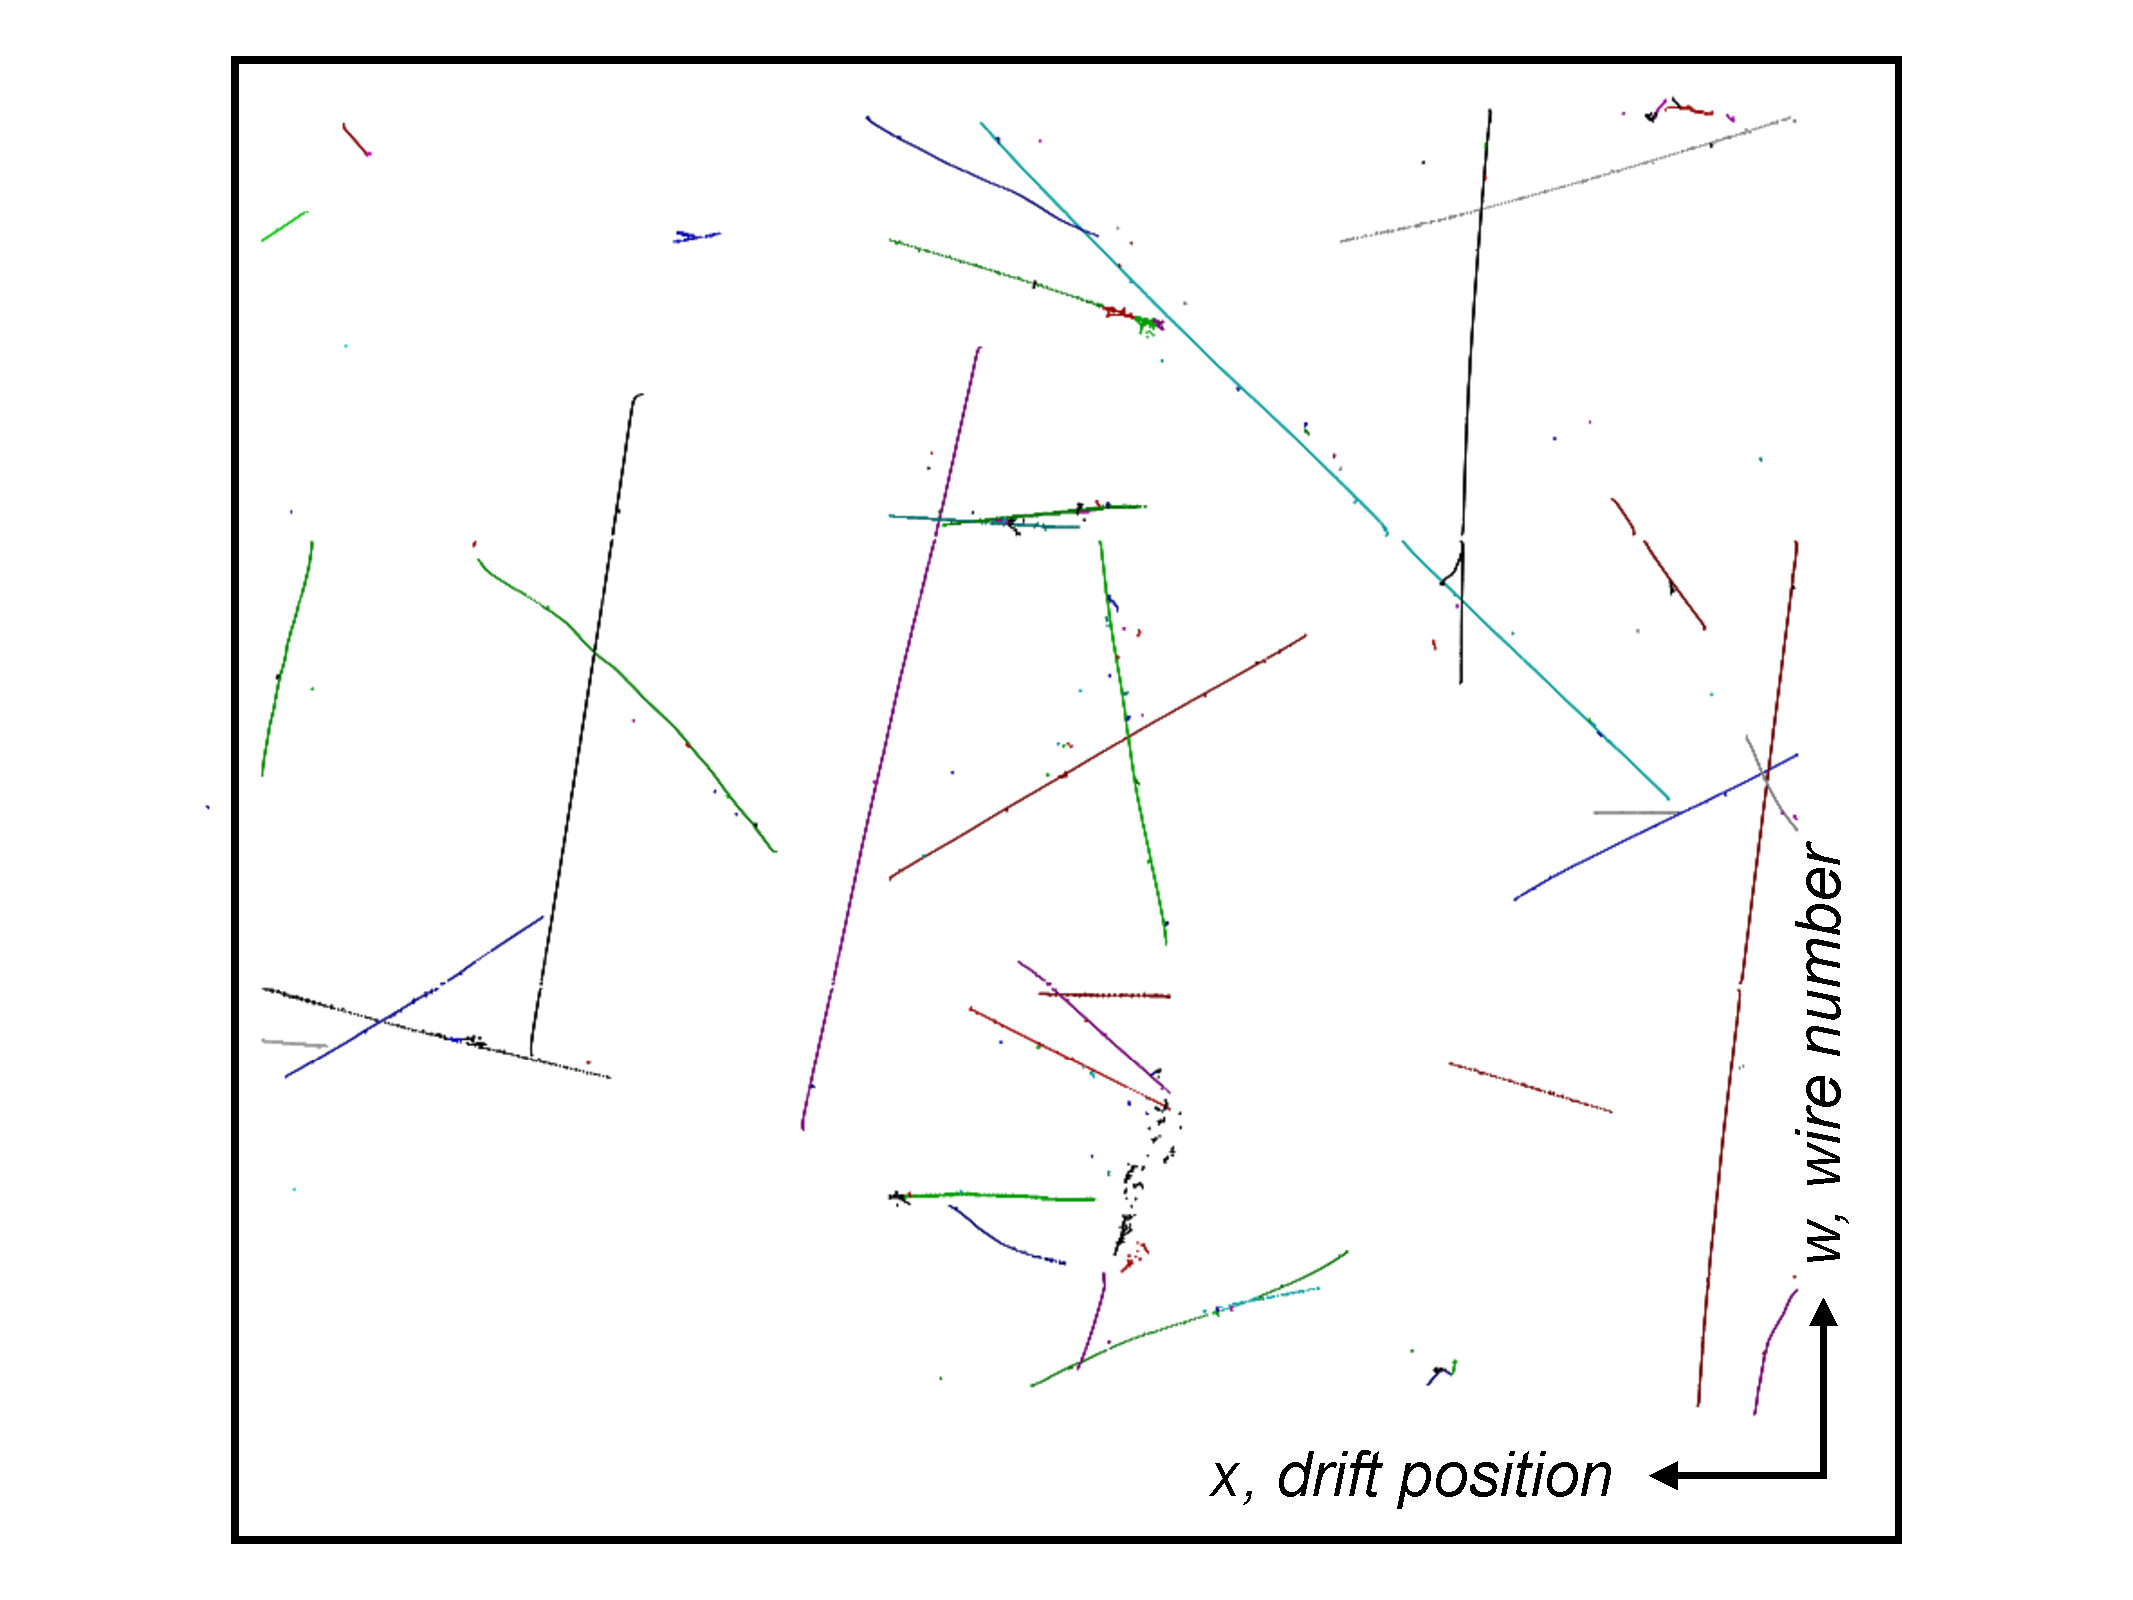
\includegraphics[width=0.33\textwidth,trim={3cm 0 3cm 0},clip]{Figures/EventDisplays/Data/full_event_2D_W_data.pdf}\label{fig:examplemcrecod}} 
\caption{The reconstruction output for a candidate 1\,GeV/$c$ $\pi^{+}$ charge exchange event from ProtoDUNE-SP data run 5387. Figure~\protect\subref{fig:examplemcrecoa} shows the 3D reconstruction output, highlighting the reconstructed particle hierarchy identified as the test-beam particle interaction: the reconstructed beam $\pi^+$ in purple comes from the left before interacting to produce two visible reconstructed $\pi^0$ decay photons in red and black. Figures \protect\subref{fig:examplemcrecob}, \protect\subref{fig:examplemcrecoc} and \protect\subref{fig:examplemcrecod} show the $u$, $v$ and $w$ view hits respectively for the fully reconstructed event.}
\label{fig:examplemcreco}
\end{figure*}

The final consolidated event that is output from Pandora contains $N$ cosmic-ray muon hierarchies, consisting of clear cosmic-ray muons and those from slices not passing the beam particle identification, and $M$ beam-particle hierarchies, one from each slice passing the beam particle slice selection threshold.

\section{Simulated and Experimental Data}
\label{sec:datadescription}
Each event in simulation and data corresponds to one 3\,ms readout window of the detector, where the readout was initiated by the triggered test-beam particle. In addition, a number of background particles of both cosmic-ray and test-beam origin also traverse the detector, as shown in Fig.~\ref{fig:eventdecomp}.

The test-beam particle generation uses a GEANT4 simulation of the beamline~\cite{PhysRevAccelBeams.20.111001,PhysRevAccelBeams.22.061003}. The triggered test-beam particle is placed into the event with $t_0=t_\textrm{trigger}=0$ and other beam interactions are overlaid at random times, assuming a uniform distribution, to give background beam interactions spanning the entire 3\,ms detector readout window. Cosmic rays are simulated using CORSIKA \texttt{v7.4}~\cite{corsika} and are generated over a 6\,ms time range (centred on the trigger time) in order to completely cover the entire 3\,ms detector readout window. The simulation of particle propagation and interaction in the ProtoDUNE-SP detector is also performed by GEANT4, and the detector response simulation was performed using LArSoft \texttt{v08\_27\_01}~\cite{Church:2013hea}. The Pandora pattern recognition was performed using LArPandoraContent version \texttt{v03\_15\_02}, which in turn depends on version \texttt{v03\_03\_02} of the Pandora SDK.

The experimental test-beam data samples considered in this article were collected from August 2018 to December 2018. Due to time constraints, test-beam data were collected only in the positive polarity mode at five different particle momentum settings: 1, 2, 3, 6 and 7\,GeV/$c$. For this reason, only simulated interactions at these same five momentum settings are shown in this article.

Both data and simulation events go through signal processing and hit finding stages, as described in Ref.~\cite{proto_performance}. The events are input into Pandora after the reconstruction of hits from the signals identified on the detector readout wires. The average time taken to reconstruct a full ProtoDUNE-SP event with Pandora using the LArSoft framework is approximately 40\,s on an Intel Core Processor (Broadwell) 2.3\,GHz CPU while using an average of 2.8\,GB of memory.

\section{Cosmic Ray Reconstruction Performance}
\label{sec:cosmicrecoperformance}

The performance of the event reconstruction is first evaluated using the simulation and then compared to the experimental data. The method presented here to evaluate the performance of ProtoDUNE-SP event reconstruction mirrors the approach used in MicroBooNE~\cite{pandorauboone}. This involves matching Monte-Carlo (MC) particles with reconstructed particles based on the number of \textit{shared hits}, which are those hits common to the reconstructed and true particles.
 
Selection criteria are applied to ensure that the MC particles are ``reconstructable'' and can be included in the performance metrics. The MC particles are required to produce at least 15 hits in the detector, with at least five hits in at least two of the three readout views. Furthermore, MC particle hits produced by non-primary neutrons, and photons produced by track-like primaries, that deposit energy a long way from the primary particle are removed from the matching criteria.

Matches between reconstructed and MC particles are made on a per-event basis by finding the match involving the largest number of shared hits between the reconstructed and MC particle. Once this match is made the reconstructed and MC particles are declared unavailable, preventing further matches being made to either particle. This process is then repeated for all remaining particles in the event. At this stage all reconstructed and MC particles have at most one match. Any remaining reconstructed particles that have no match are associated to the MC particle (that by definition must already have a single match) with which they share the most hits, irrespective of the number of matches the MC particle already has.

Once the reconstructed particles have been matched to the MC particles, the following metrics can be defined for each matched pair:
\begin{itemize}
\item \textbf{Efficiency}: The fraction of MC particles that are matched to at least one reconstructed particle. The Clopper-Pearson method~\cite{clopperPearson} is used to calculate the confidence interval on efficiency measurements presented in this article.
\item \textbf{Purity}: The fraction of hits in the reconstructed particle that are shared with the MC particle.
\item \textbf{Completeness}: The fraction of hits in the MC particle that are shared with the reconstructed particle.
\end{itemize}

When MC particles are matched to reconstructed particles, matches are only made if the purity of the match is greater than 50\% in order to ensure that the reconstructed particle is predominantly associated with a single MC particle. Furthermore, a completeness of 10\% is required in order to veto low-quality matches. These cuts are not applied when reporting the completeness and purity of matches.  

\subsection{Simulation Reconstruction Performance}
\label{sec:crmetrics}
The left panel of Figure~\ref{fig:crrecoeff} shows the reconstruction efficiency for cosmic-ray muons as a function of the total number of true hits produced by the particle in the detector (including hits from delta-ray showers and Michel electrons). The overall integrated reconstruction efficiency for cosmic-ray muons is $95.73 \pm 0.03$\%. The reconstruction efficiency increases as a function of the number of hits, rising from 50\% for 15 hits up to 99\% for particles producing more than 400 hits. The reconstruction inefficiency for particles producing fewer hits is due to cosmic-ray muons being absorbed into larger neighbouring particles. This is more common for cosmic-ray muons producing a small number of hits, but it is also possible for large cosmic-ray muons if the surrounding topology is sufficiently complex.

\begin{figure}[htb]
 \centering
 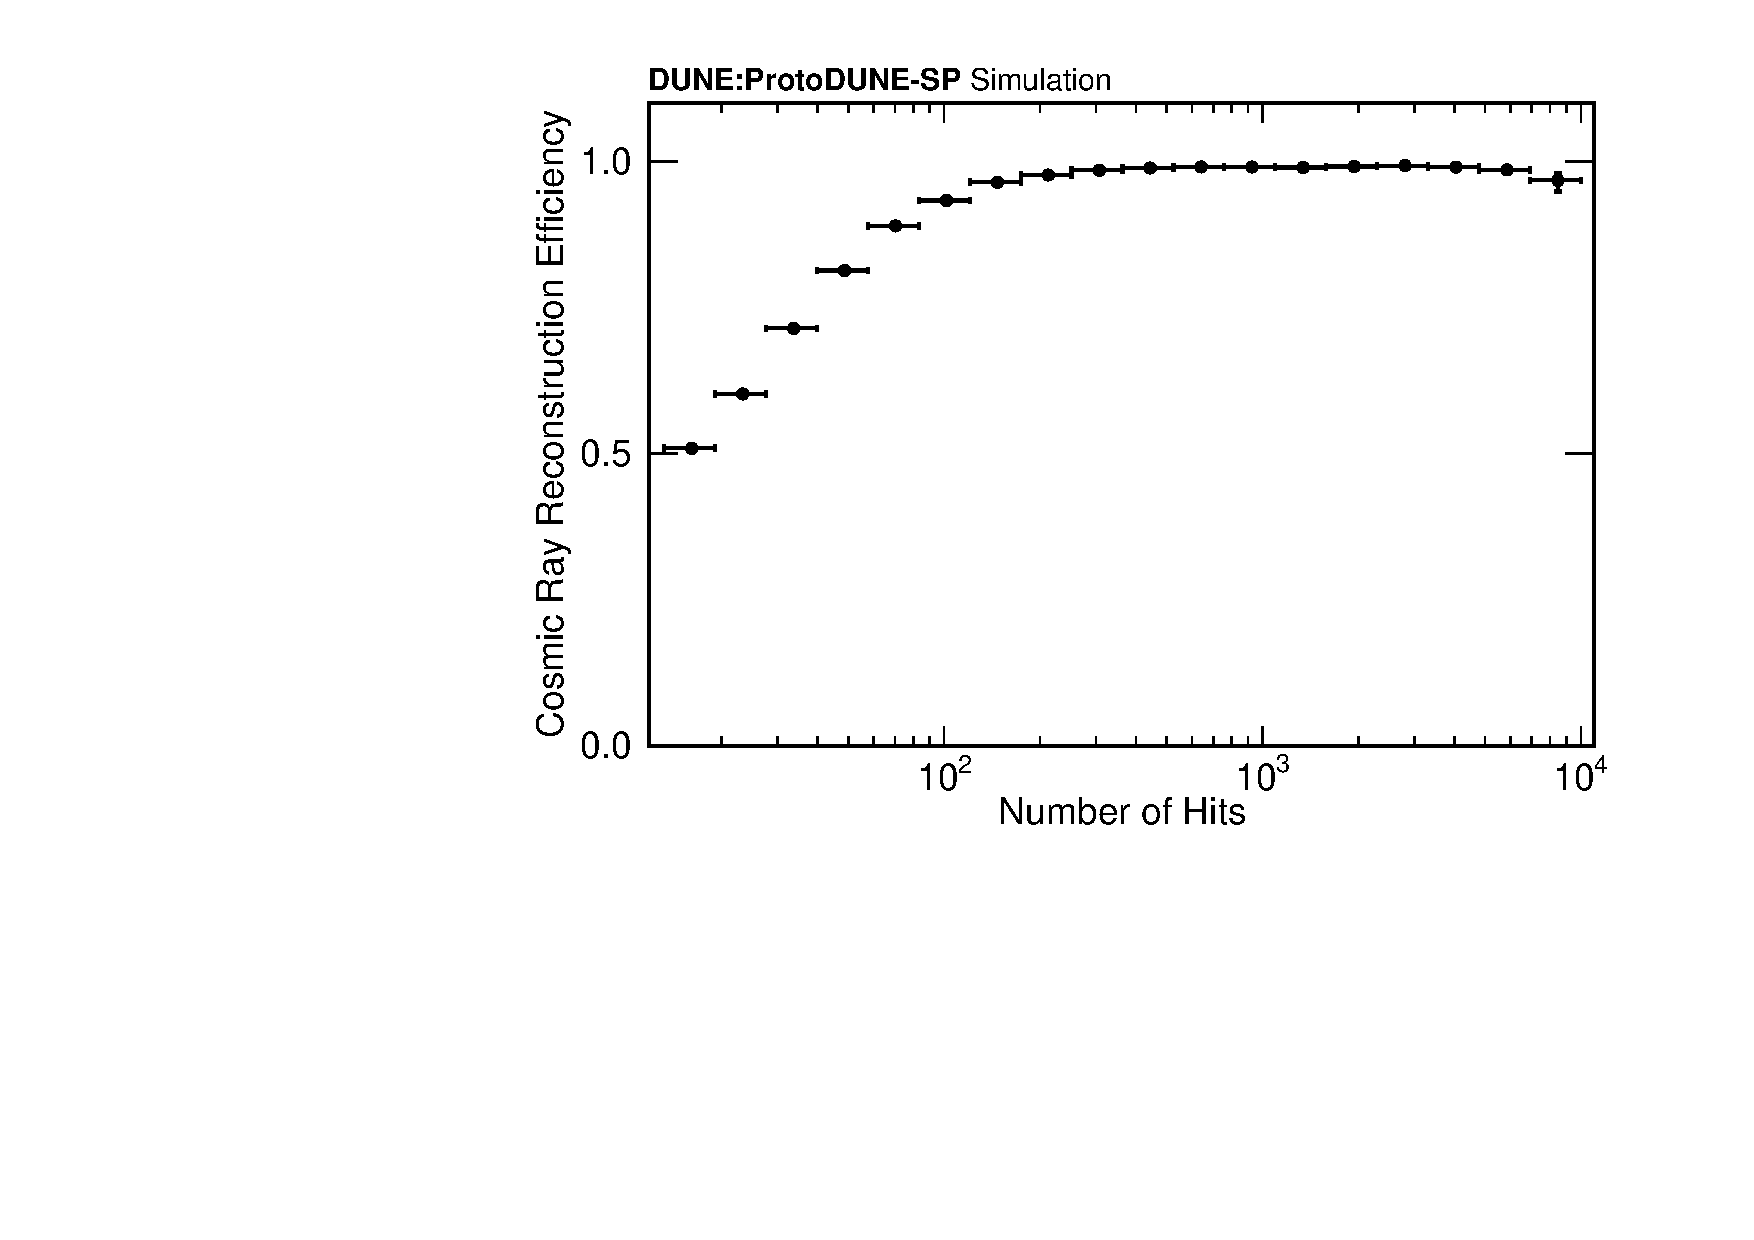
\includegraphics[width=0.48\textwidth,trim={0 0 1cm 0},clip]{Figures/Metrics/MC/Cosmics/CosmicRayEfficiencyVsNHits.pdf}
 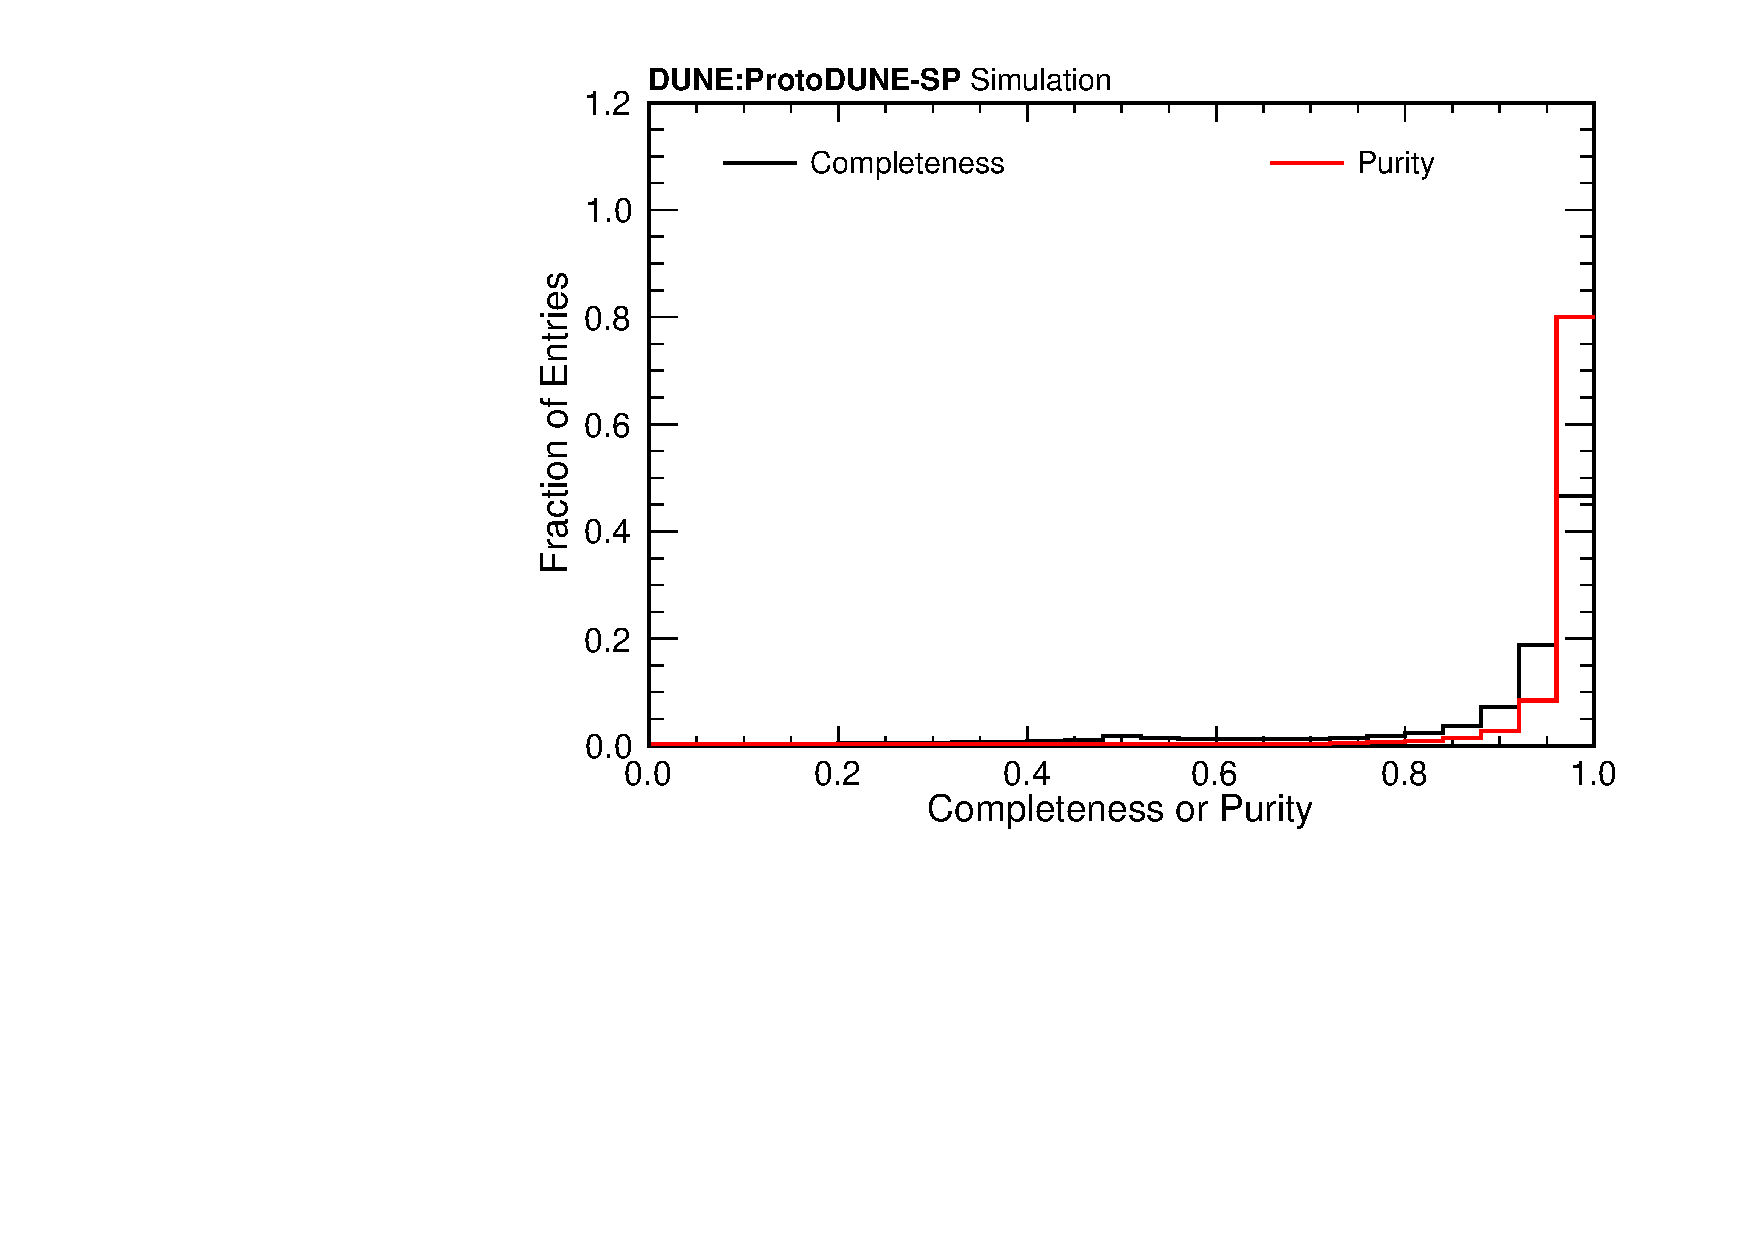
\includegraphics[width=0.48\textwidth,trim={0 0 1cm 0},clip]{Figures/Metrics/MC/Cosmics/CosmicRayCompletenessAndPurity.pdf}
 \caption{Left: the reconstruction efficiency for simulated cosmic-ray muons as a function of the true number of hits (summed over the three readout views) produced by the cosmic-ray muon. Right: the completeness and purity of the reconstructed cosmic-ray muons.}
 \label{fig:crrecoeff}
\end{figure}


The completeness and purity of the reconstructed cosmic-ray muons are shown in right panel of Fig.~\ref{fig:crrecoeff}, both of which have very clear peaks at one. These figures show that 97.6\% of reconstructed cosmic-ray muons have a purity greater than 80\% and 81.9\% of reconstructed cosmic-ray muons have a completeness greater than 80\%. The tail on the low side of the completeness distribution
 is caused by the reconstruction splitting up a cosmic-ray muon track into two distinct particles. Approximately 8\% of the cosmic-ray muons are matched to two reconstructed particles, meaning that the reconstruction failed to reconstruct the particle as a single object. This can happen for a number of reasons, including failing to stitch the tracks at the drift volume boundaries, crossing cosmic-ray topologies and large delta-ray showers overlapping with with the muon tracks. The purity is typically close to 100\%, which indicates merging distinct cosmic-ray muons together is unlikely.

It is possible to identify the time, $t_{0}$, that a cosmic-ray muon enters the LArTPC if the reconstructed particle was stitched between drift volumes by the process discussed in Sec.~\ref{sec:pandoracosmic} and shown visually in Fig.~\ref{fig:stitching}. The distribution of the $t_{0}$ residual, the difference between the reconstructed and true value of $t_{0}$, for stitched cosmic-ray muons is shown in Fig.~\ref{fig:crt0res}. The dashed black histogram shows the case where no space charge distortion was applied to the simulation and the distribution is centred on zero, as expected. Once space charge is included (the solid black distribution), a number of features become apparent when considering the cathode- (blue) and APA-stitched (red) components separately. The APA-stitched distribution remains centred on zero because the charge deposited close to the APA travels only a short distance and is unaffected by space charge distortions. Conversely, charges drifting from the cathode are maximally affected since they travel the entire drift distance, resulting in a distribution that is shifted by a few microseconds. The effect of space charge is illustrated in Fig.~\ref{fig:spacechargetrack}, which shows a diagram of a reconstructed cathode-stitched cosmic-ray muon compared to the true trajectory. The bowing effect results in an overestimation of the shift in the drift direction, and hence the reconstructed $t_{0}$. The magnitude of the SCE varies across the LArTPC resulting in a broadening of the $t_{0}$ residual distribution. Finally, the asymmetric nature of the space charge distortions at the cathode causes a double-peak structure for cathode-stitched tracks, depending on whether the particle crossed the cathode from positive to negative $x$ or vice versa.

\begin{figure}[htb]
\centering
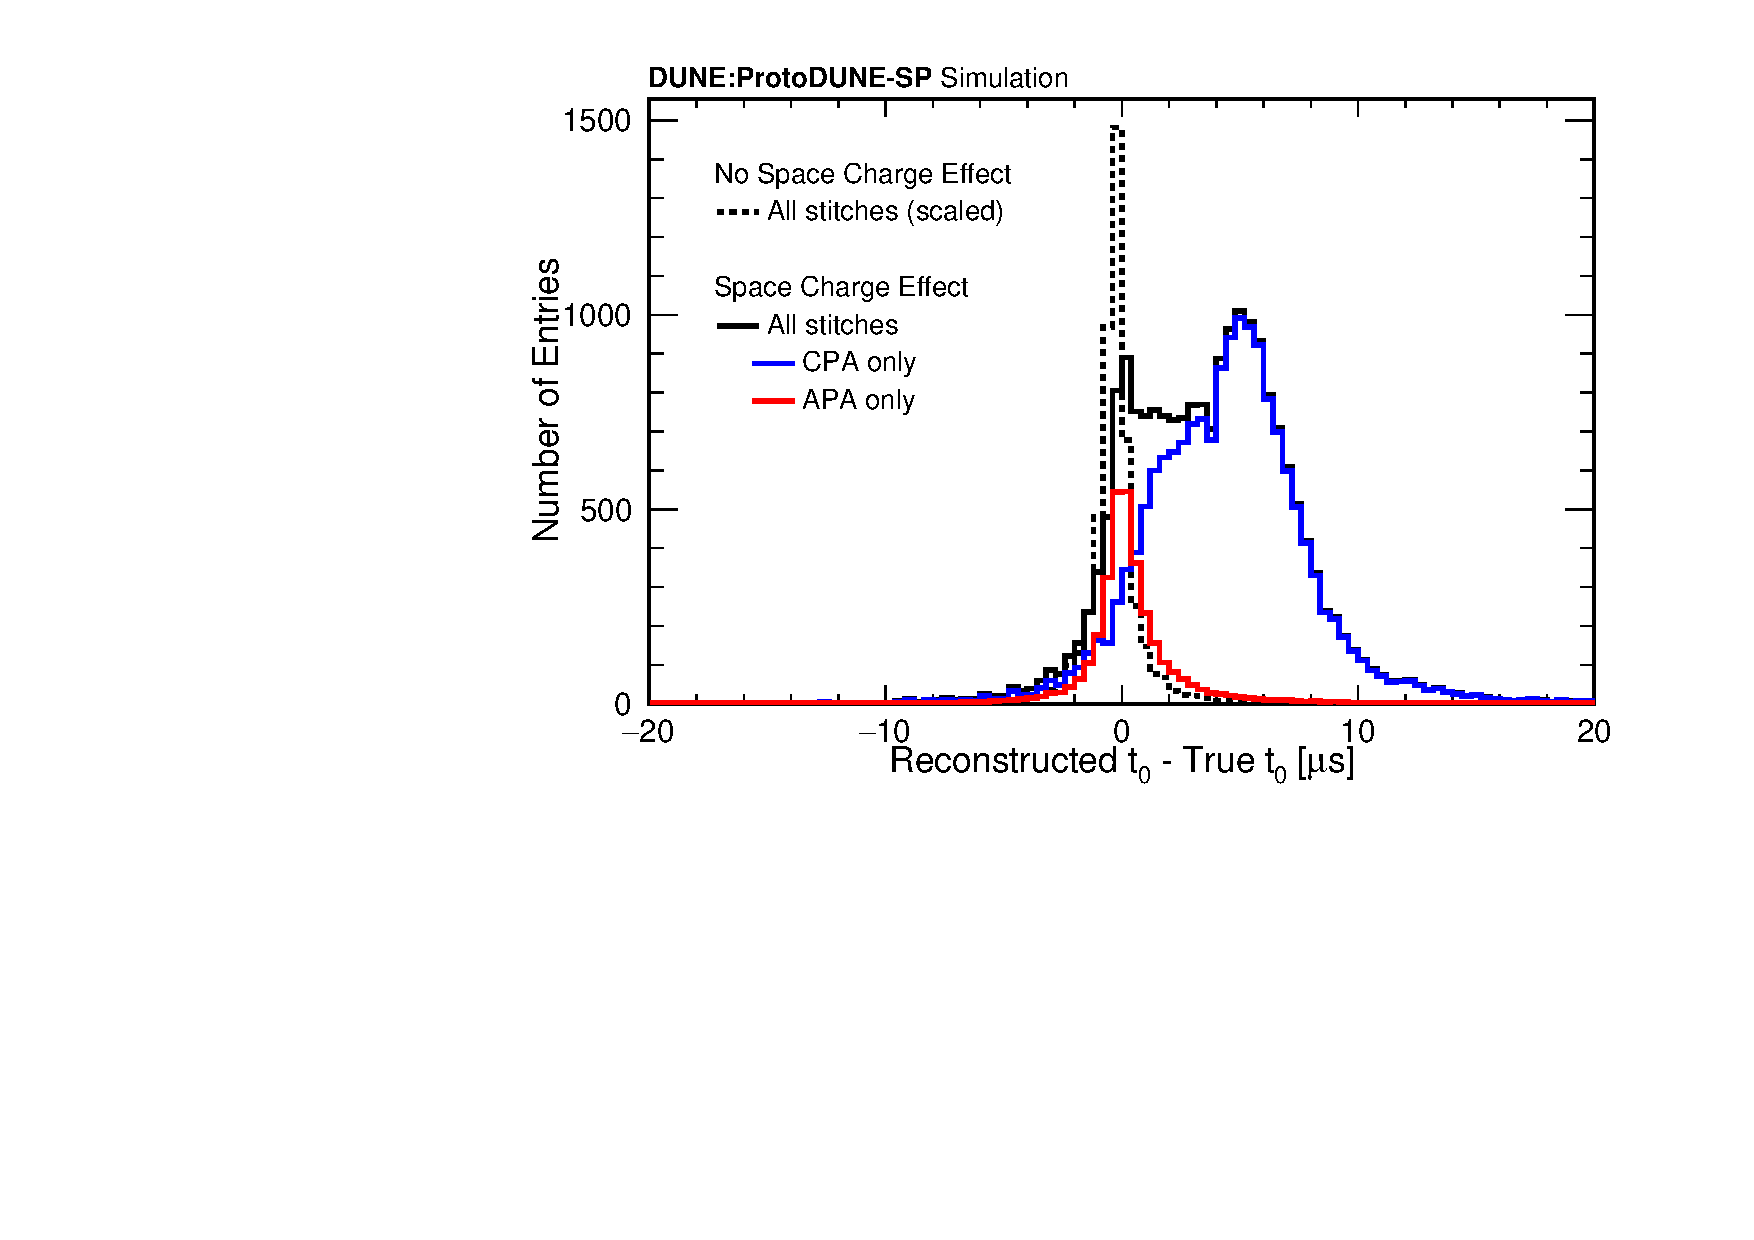
\includegraphics[width=0.60\textwidth]{Figures/Metrics/MC/Cosmics/prod2_Pandora_T0_Residual.pdf}
\caption{The difference between the reconstructed and true $t_{0}$ for simulated cosmic-ray muons that have been stitched at either the CPA or APA with (solid black) or without (dashed black) space charge distortions. The black distribution is shown divided into the CPA- (blue) and APA-stitched (red) components. A time difference of 20\,$\upmu$s corresponds to shift of about 3\,cm in the drift direction.}
\label{fig:crt0res}
\end{figure}

\begin{figure}[htb]
\centering
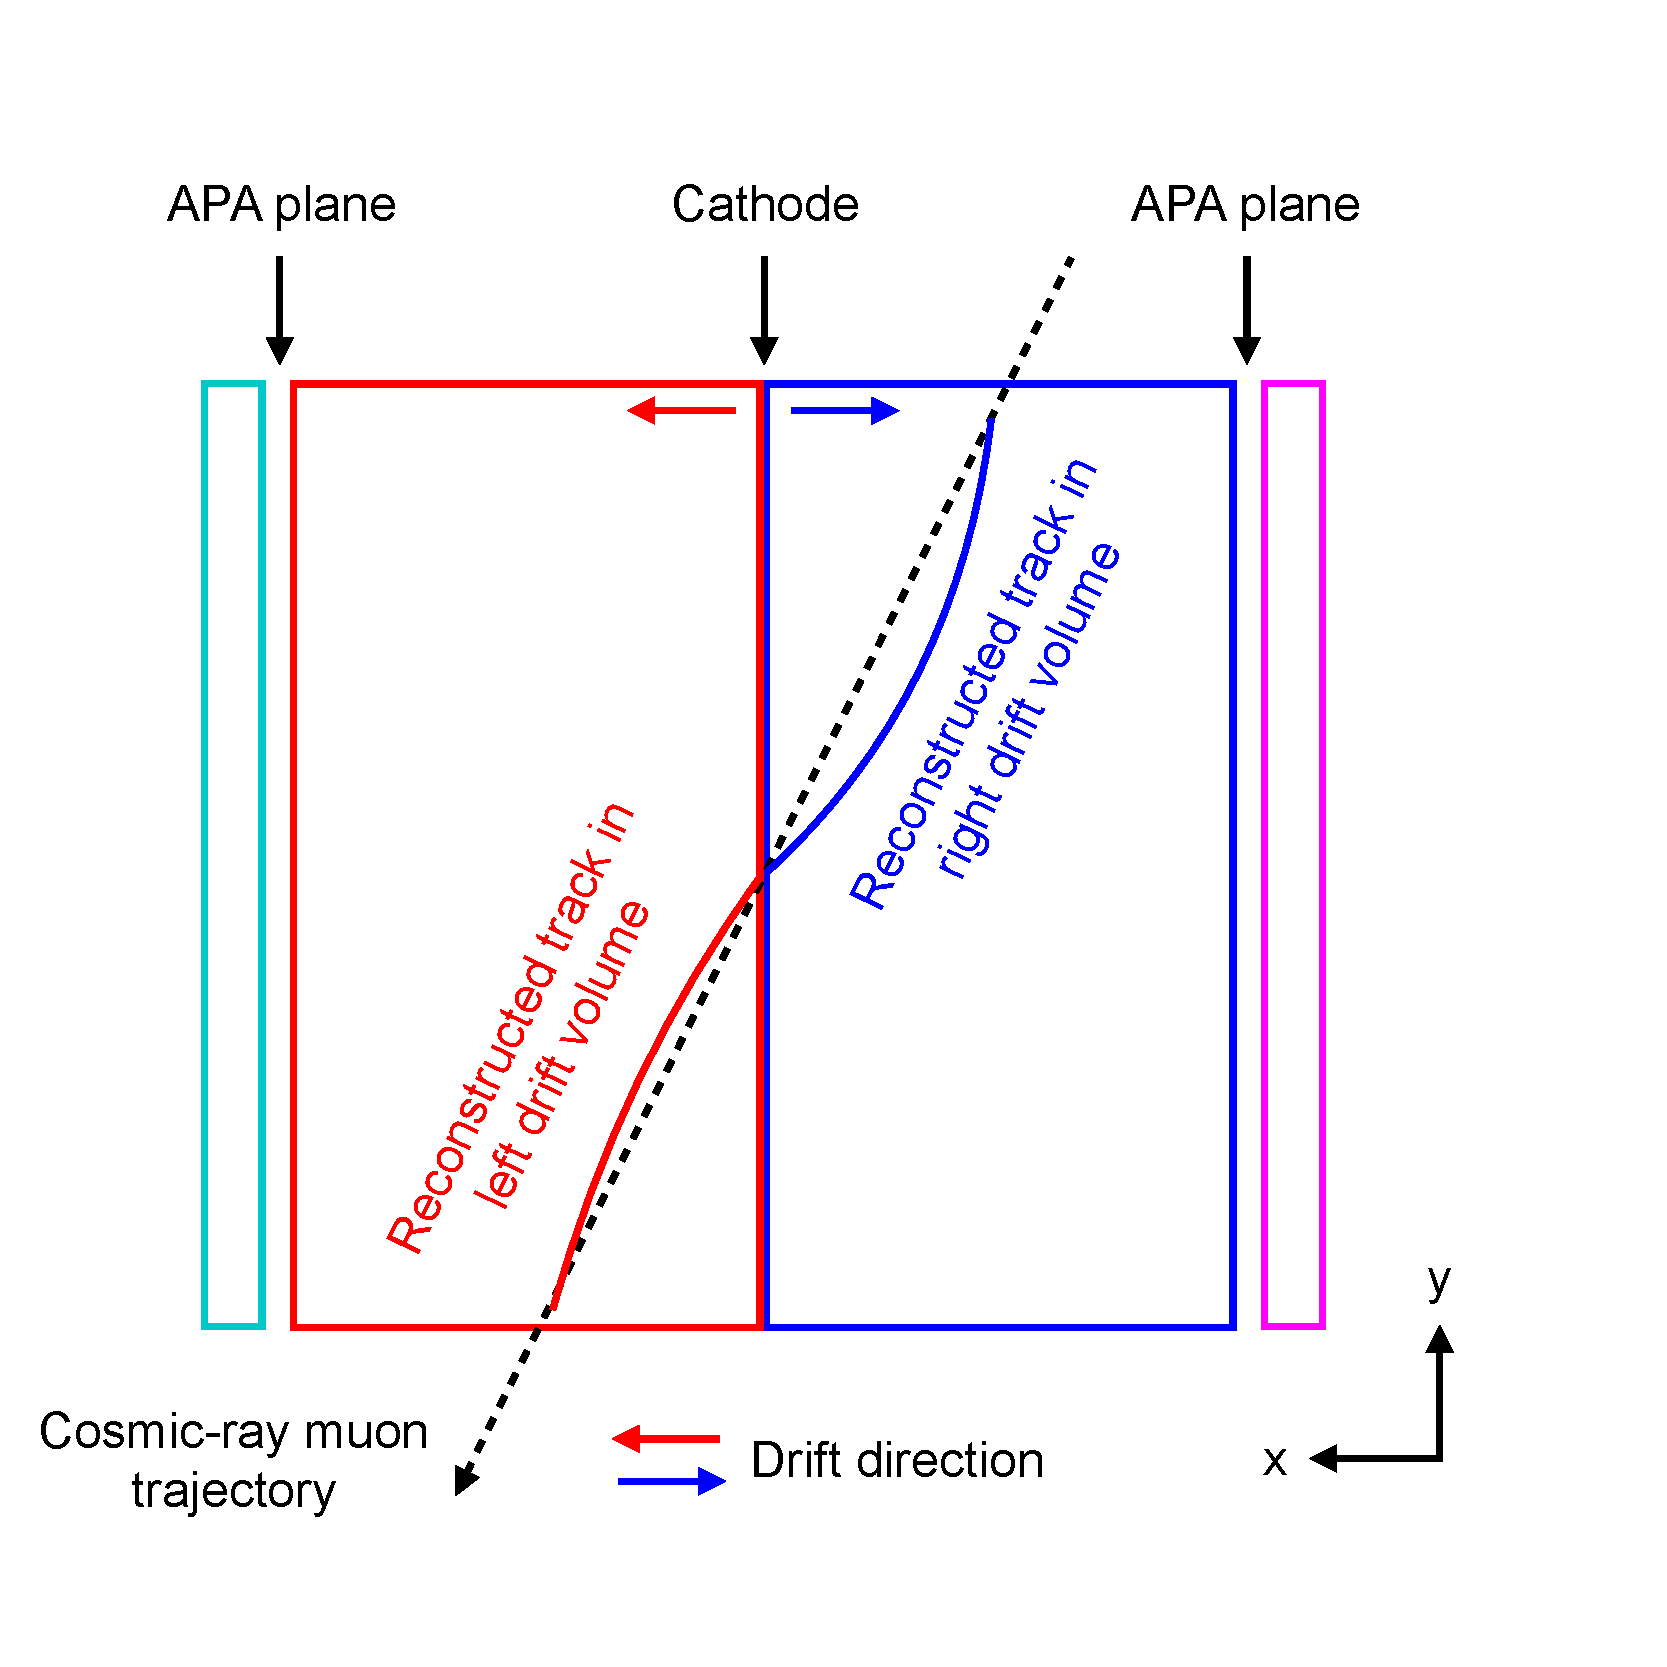
\includegraphics[width=0.48\textwidth]{Figures/Diagram/SCE_Schematic_FromTop.pdf}
\caption{A schematic diagram of how the space charge effect causes distortions to the reconstructed tracks in both the drift direction and the orthogonal directions. For clarity, the amount of distortion has been exaggerated. The red and blue show the tracks reconstructed in the two central drift volumes, while the black dotted line represents the true trajectory of the cosmic-ray muon.}
\label{fig:spacechargetrack}
\end{figure}

In order to give context to the topologies that the reconstruction is faced with at ProtoDUNE-SP, an estimate of the number of cosmic-ray muons passing through the detector per event in simulation has been made. The number of reconstructed cosmic-ray muons matched, via the procedure discussed at the start of this section, to distinct cosmic-ray muon MC particles, i.e. that deposit more than 100 hits in the detector, is shown as a function of the total number of distinct cosmic-ray muons on a per-event basis in Fig.~\ref{fig:crnperevt}. The distribution shows a strong linear correlation, but the gradient is approximately 1.08, corresponding to the aforementioned 8\% of cosmic rays that were reconstructed as two particles. However, it demonstrates that on average the cosmic-ray muons are well reconstructed.
The mean number of distinct cosmic-ray muons per event is 52
, while the mean number of matched reconstructed particles to those cosmic-ray muons is 56, with negligible uncertainties. These figures demonstrate that on a per-event basis, cosmic-ray muons significantly outnumber triggered test-beam particles.

\begin{figure}
\centering
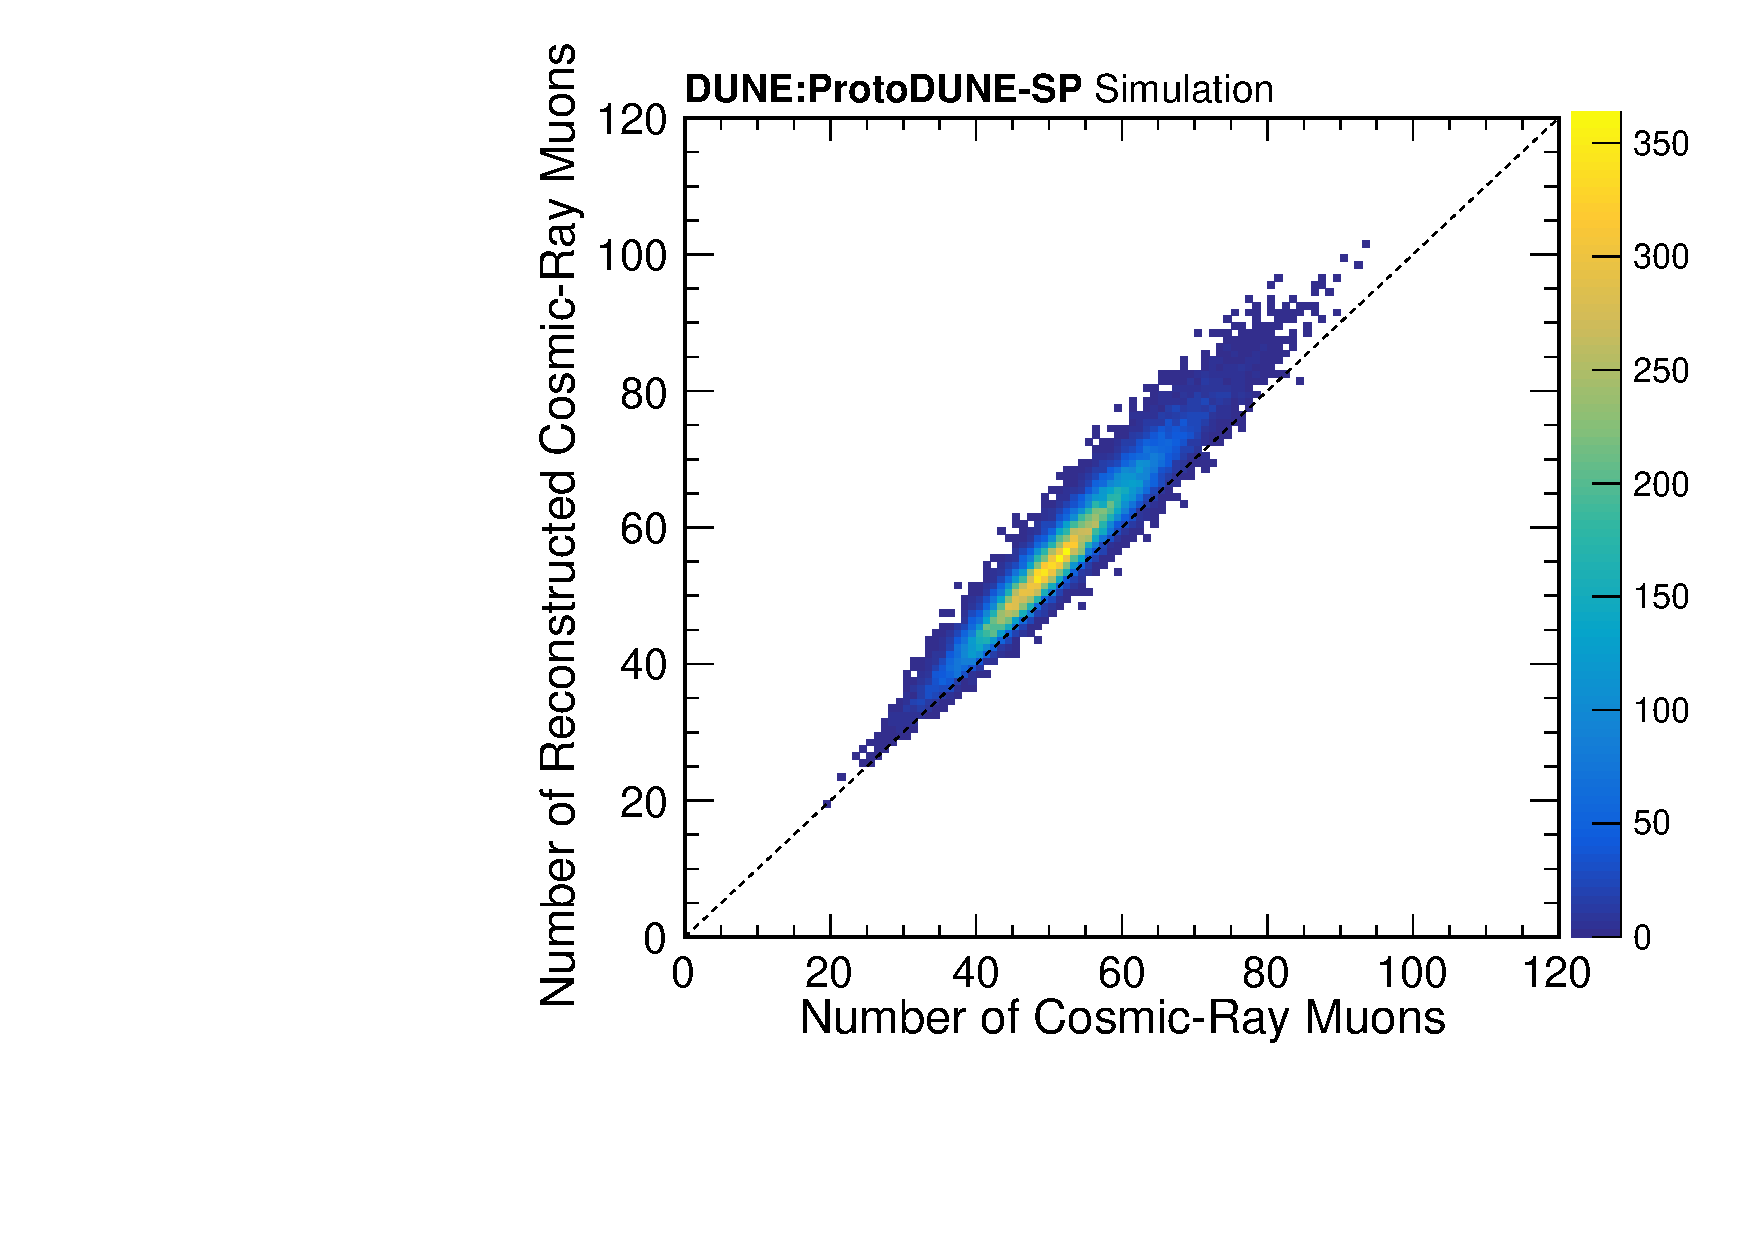
\includegraphics[width=0.48\textwidth]{Figures/Metrics/MC/Cosmics/CRMatchesCosmicRayEvent100.pdf}
\caption{The number of reconstructed cosmic-ray muons as a function of the number of true cosmic-ray muons on a per-event basis. The cosmic-ray muons were required to produce at least 100 hits in the detector.}
\label{fig:crnperevt}
\end{figure}

\subsection{Comparisons of Data and Simulation}
Reconstruction metrics for cosmic-ray muon data have also been evaluated. Figure~\ref{fig:ncrdata} shows the number of reconstructed particles tagged as distinct cosmic-ray muons per event in ProtoDUNE-SP. For a cosmic-ray muon to be tagged as distinct it must deposit at least 100 hits in the detector. This cut is applied in order to define a substantial, distinct signal in the detector. Furthermore, applying this cut yields a minimum reconstruction efficiency of \,90\%, based on the simulated efficiencies in Fig.~\ref{fig:crrecoeff}, which ensures this metric gives an accurate reflection of the true number of distinct cosmic-ray muons entering ProtoDUNE-SP.

Approximately 5\% fewer cosmic-ray muons are reconstructed per event in data than simulation, with the data distribution peaking at $51.8\pm0.1$ and the simulated distribution peaking at $54.9\pm0.1$. This could be due to an overestimation of the cosmic ray flux in the simulation. Preliminary studies show that additional geometric selection criteria significantly improve the agreement in the mean number of reconstructed particles between data and simulation.

\begin{figure}[htb]
\centering
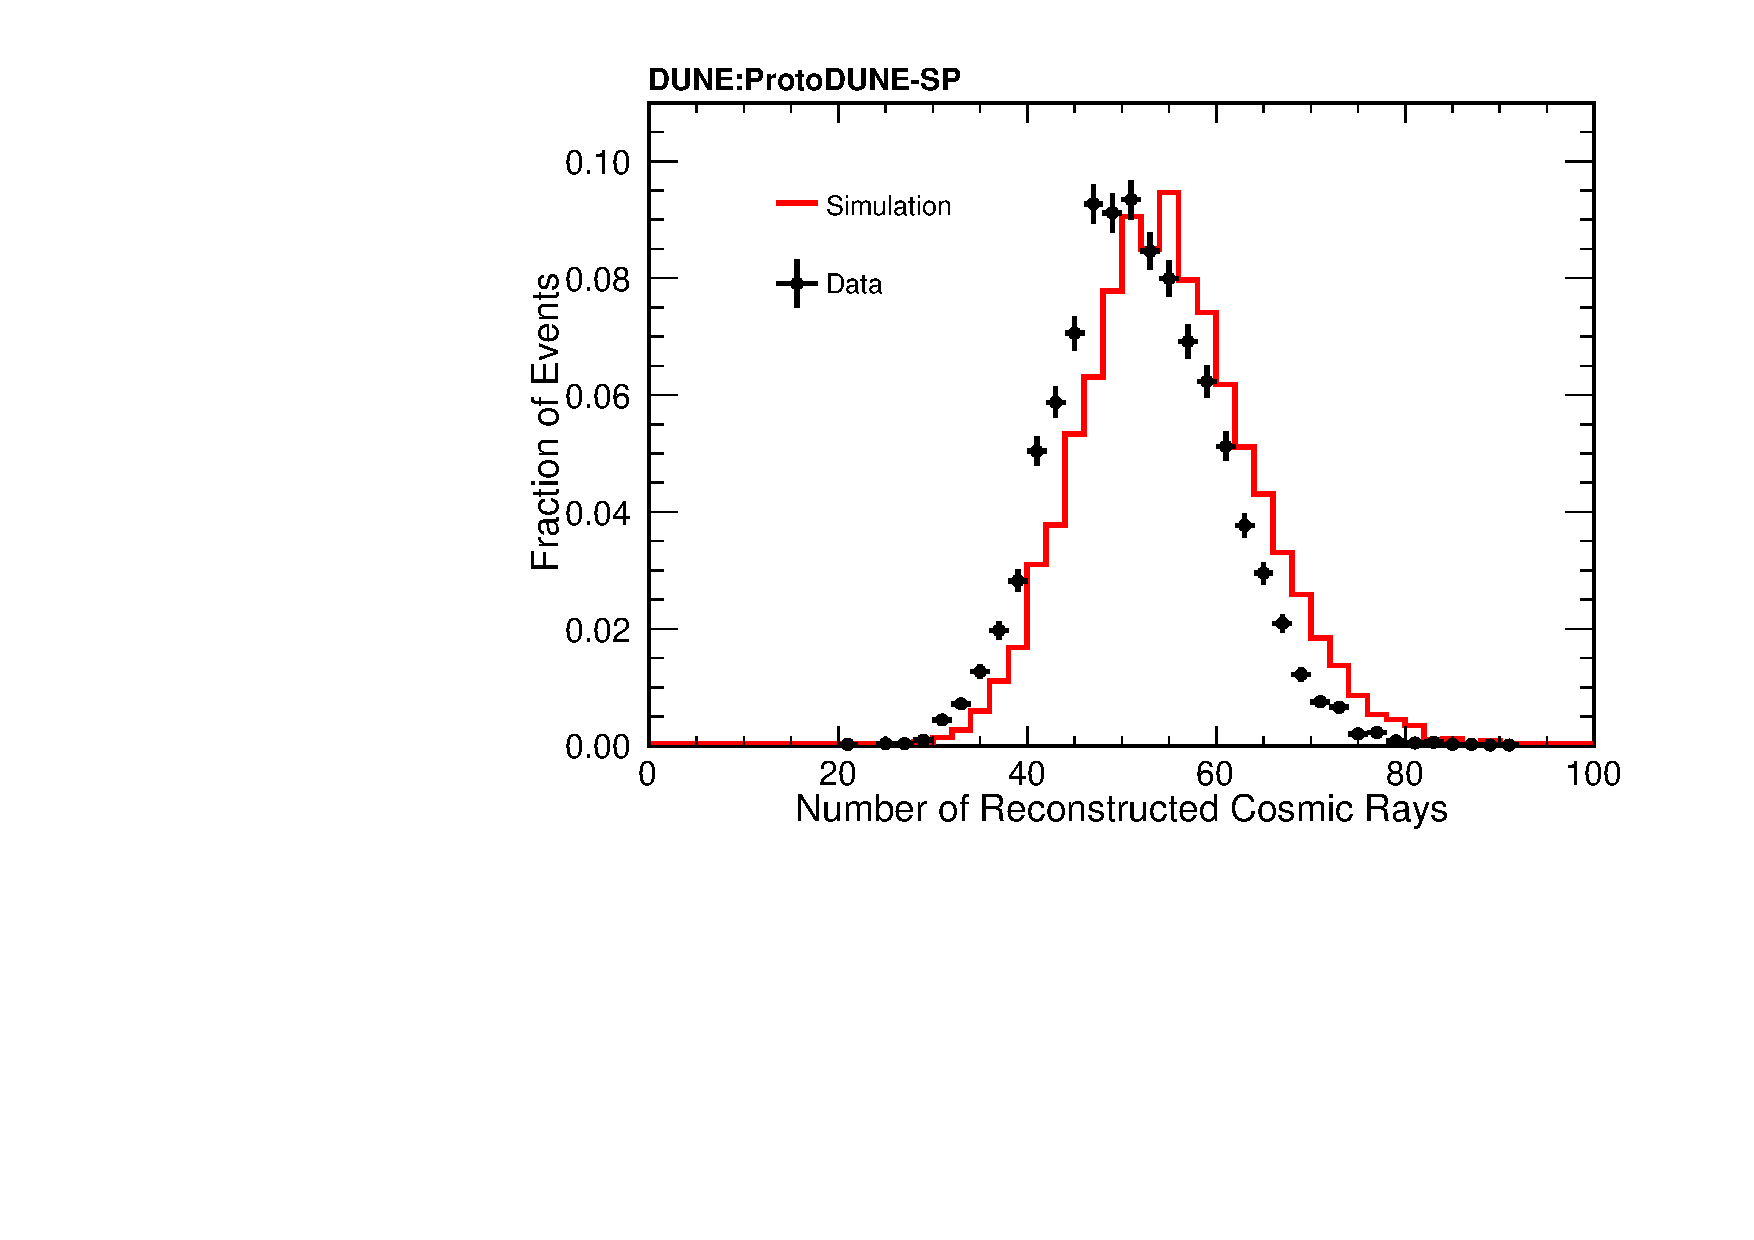
\includegraphics[width=0.48\textwidth]{Figures/Metrics/Data/Cosmics/prod2_pandora_nCosmic_data_mc.pdf}
\caption{The number of reconstructed distinct cosmic-ray muon particles per event for data (black) and simulation (red). The cosmic-ray muons were required to produce at least 100 hits in the detector.}
\label{fig:ncrdata}
\end{figure}

\begin{figure}[htb]
\centering
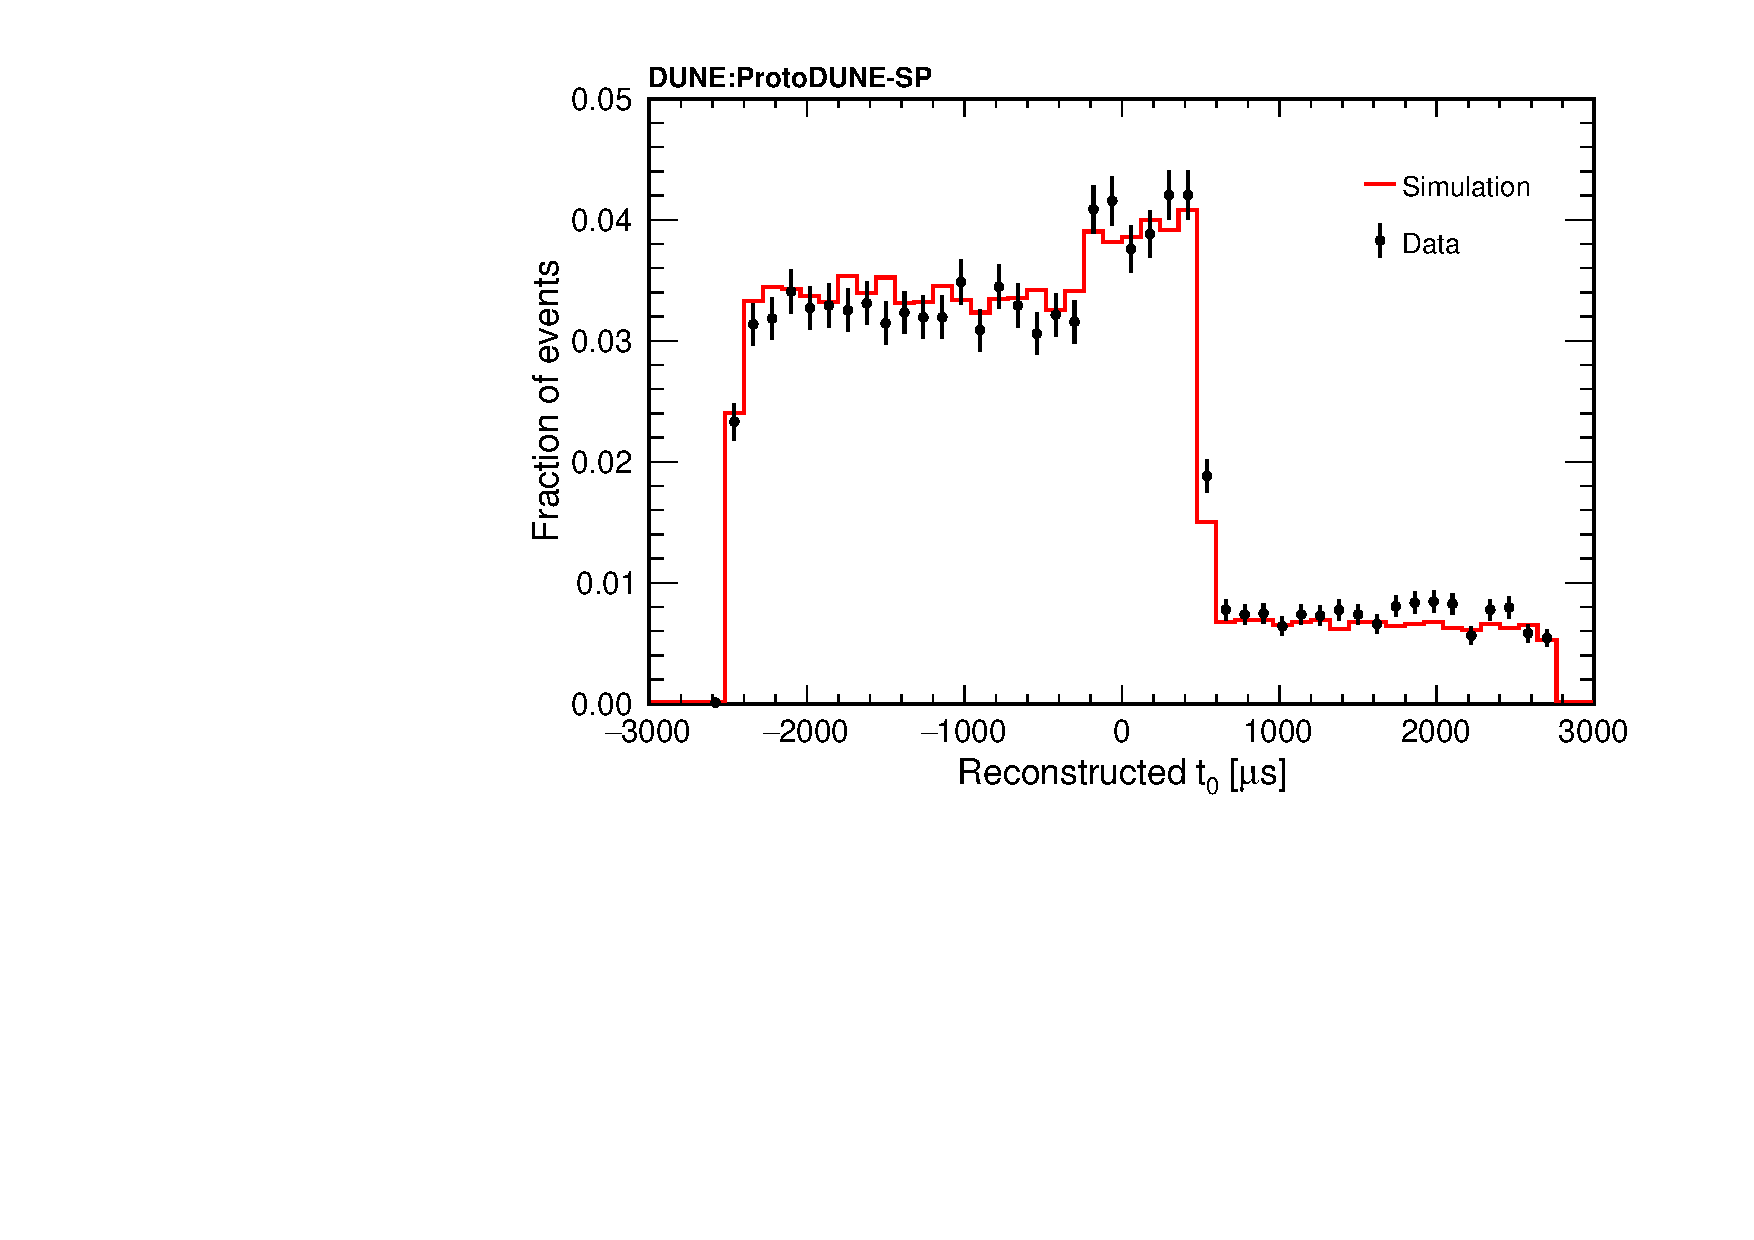
\includegraphics[width=0.48\textwidth]{Figures/Metrics/Data/Cosmics/StitchedT0.pdf}
\caption{The reconstructed $t_{0}$ distribution in ProtoDUNE-SP for cathode crossing and anode crossing cosmic-ray muons obtained from the Pandora stitching process in data and simulation. The distributions have been area normalised for comparison. Figure reproduced from Ref.~\cite{proto_performance}.}
\label{fig:recoT0data}
\end{figure}

The distribution of the reconstructed $t_{0}$ values for cathode crossing and anode crossing cosmic-ray muons is shown in Fig.~\ref{fig:recoT0data}. The range of this distribution can be predicted by considering the readout time window ($-$250\,$\upmu$s to 2750\,$\upmu$s) and the time for charge to drift from the cathode to the APAs (2250\,$\upmu$s). The cathode-crossing cosmic-ray muons have $t_0$ values in the range $-$2500\,$\upmu$s to 500\,$\upmu$s: the lower value is the start of the readout window minus the drift time, and the upper value is the end of the readout window minus the drift time. For APA-crossing cosmic rays, the $t_0$ values fall only within the readout window. Thus, the total distribution spans the range $-2500\,\upmu$s $< t_0 < 2750\,\upmu$s. Good agreement is seen between data and simulation and the distributions fall within the expected time window predicted above.

\section{Test-Beam Reconstruction Performance}
\label{sec:testbeamrecoperformance}

The reconstruction and identification of the triggered test-beam particle is a key part of the hadron cross-section analyses at ProtoDUNE-SP. This section evaluates the performance on simulation and then provides comparisons between simulation and experimental data. As described in Sec.~\ref{sec:datadescription}, triggered test-beam particle interactions were produced with beam momenta of 1, 2, 3, 6 and 7\,GeV/$c$, and the full events included additional beam halo particles and cosmic rays.

\subsection{Simulation Reconstruction Performance}
\label{sec:beam_mc}

The reconstruction of the triggered test-beam particle end point is of particular interest for cross-section analyses because it is critical to know where the particle either interacted or stopped~\cite{Gramellini:2018mjg,LArIAT:2021yix}. The differences between the reconstructed and true values for the end position coordinates of these particles are shown in Fig.~\ref{fig:end_point_res} for 1\,GeV protons and positively charged pions. The end point was corrected for SCE distortions using the procedure described in Ref.~\cite{proto_performance} and the resulting distributions are narrow and centred on zero, indicating good resolution and low bias. The right distribution shows the difference between the reconstructed and true positions in 3D, where $68\%$ of the beam particle end points are reconstructed within 2\,cm of the true value. 
 
 \begin{figure}[htb]
    \centering
    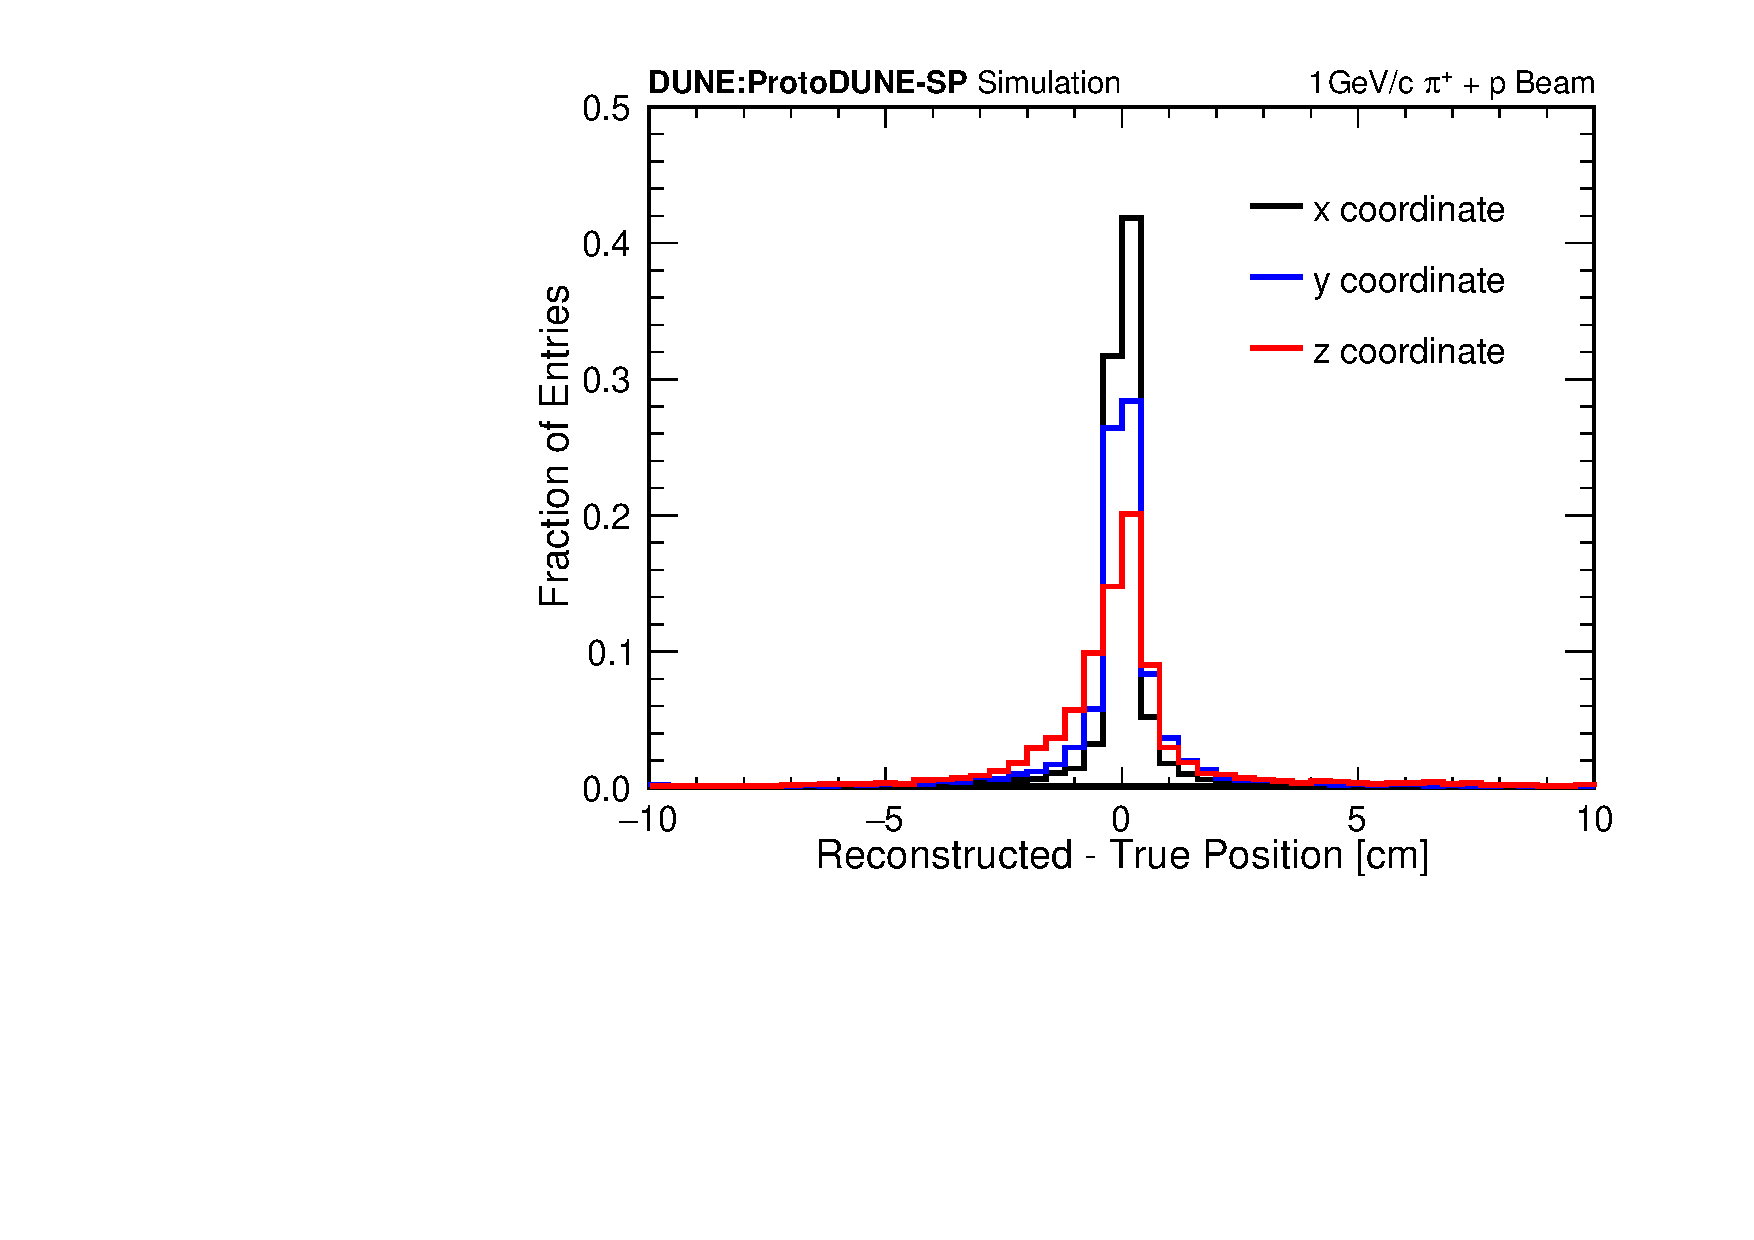
\includegraphics[width=0.48\textwidth,trim={0 0 0.5cm 0},clip]{Figures/Metrics/MC/Beam/pandora_beam_primary_end_position_residual_combined.pdf} %&
    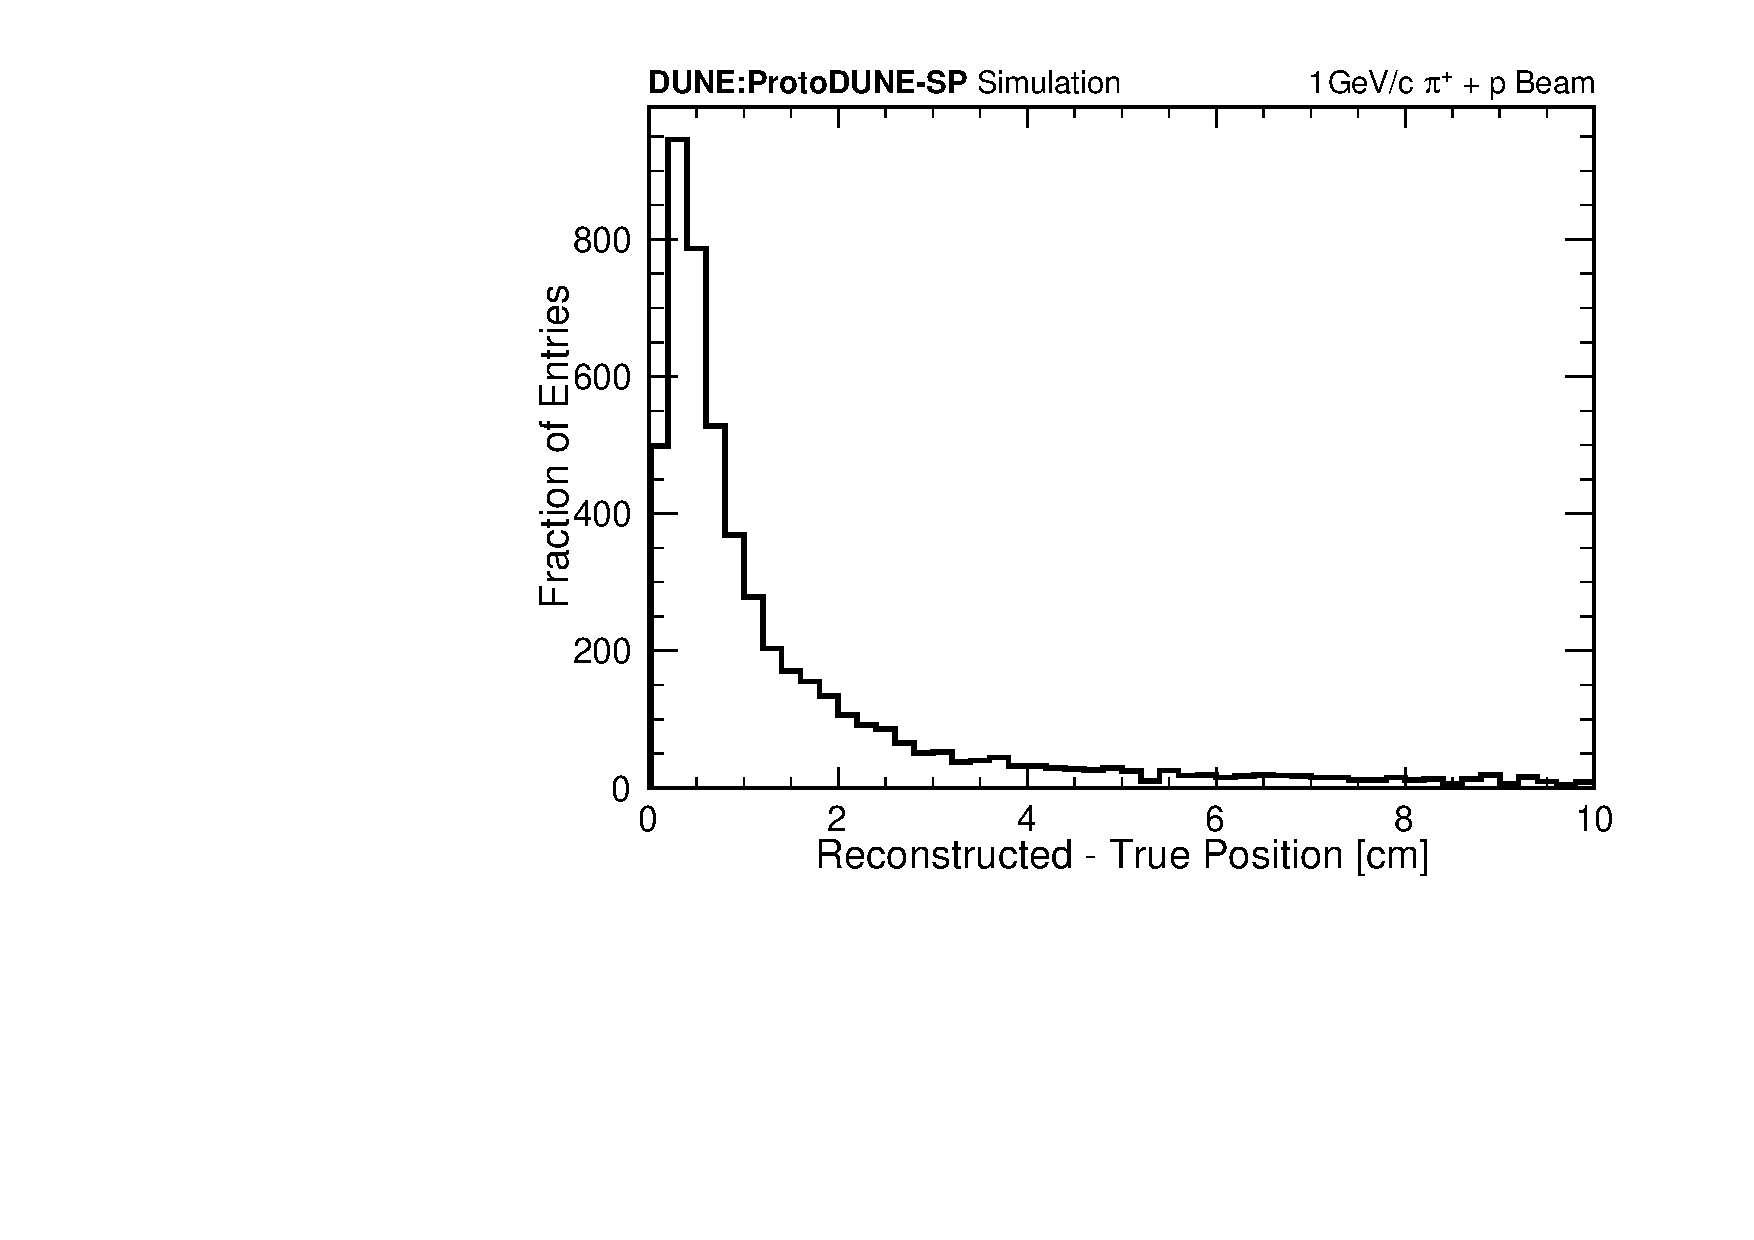
\includegraphics[width=0.48\textwidth,trim={0 0 0.5cm 0},clip]{Figures/Metrics/MC/Beam/pandora_beam_primary_end_position_residual_r.pdf}
    \caption{Left: the difference between the reconstructed and true end position of 1\,GeV/$c$ primary proton and charged pion test-beam particles shown for the $x$ (black), $y$ (blue) and $z$ (red) coordinates. Right: the three dimensional distance between the reconstructed and true end points.}
    \label{fig:end_point_res}
\end{figure}

 The efficiency to fully reconstruct triggered test-beam particles and to correctly identify them as of beam origin has been studied. In addition to the full simulation (including the triggered test-beam particle, beam-halo particles and cosmic rays), two additional simulated samples were used to understand the potential loss of efficiency due to background particles. The \textit{cosmics removed} sample has the cosmic rays removed from the event and hence consists only of the triggered test-beam particle and any beam-halo particles, and the \textit{cosmics and halo removed} sample further removes the beam-halo particles from the event, meaning only the triggered test-beam particle remains.

 Figure~\ref{fig:tbrecoeffbrkdwn} shows six distributions that visualise the reconstruction performance for the standard simulation (black), the cosmics removed sample (red), and the cosmics and halo removed sample (cyan). Each column shows, from top to bottom: the triggered test-beam particle reconstruction and identification efficiency, meaning that the particle was well reconstructed and correctly identified as being the triggered test-beam particle; and the completeness and purity of the triggered test-beam particle and subsequent hierarchy. The left column is for 1\,GeV/$c$ $\pi^+$ interactions and the right column shows 1\,GeV/$c$ $e^+$ events.

\begin{figure*}
\centering
  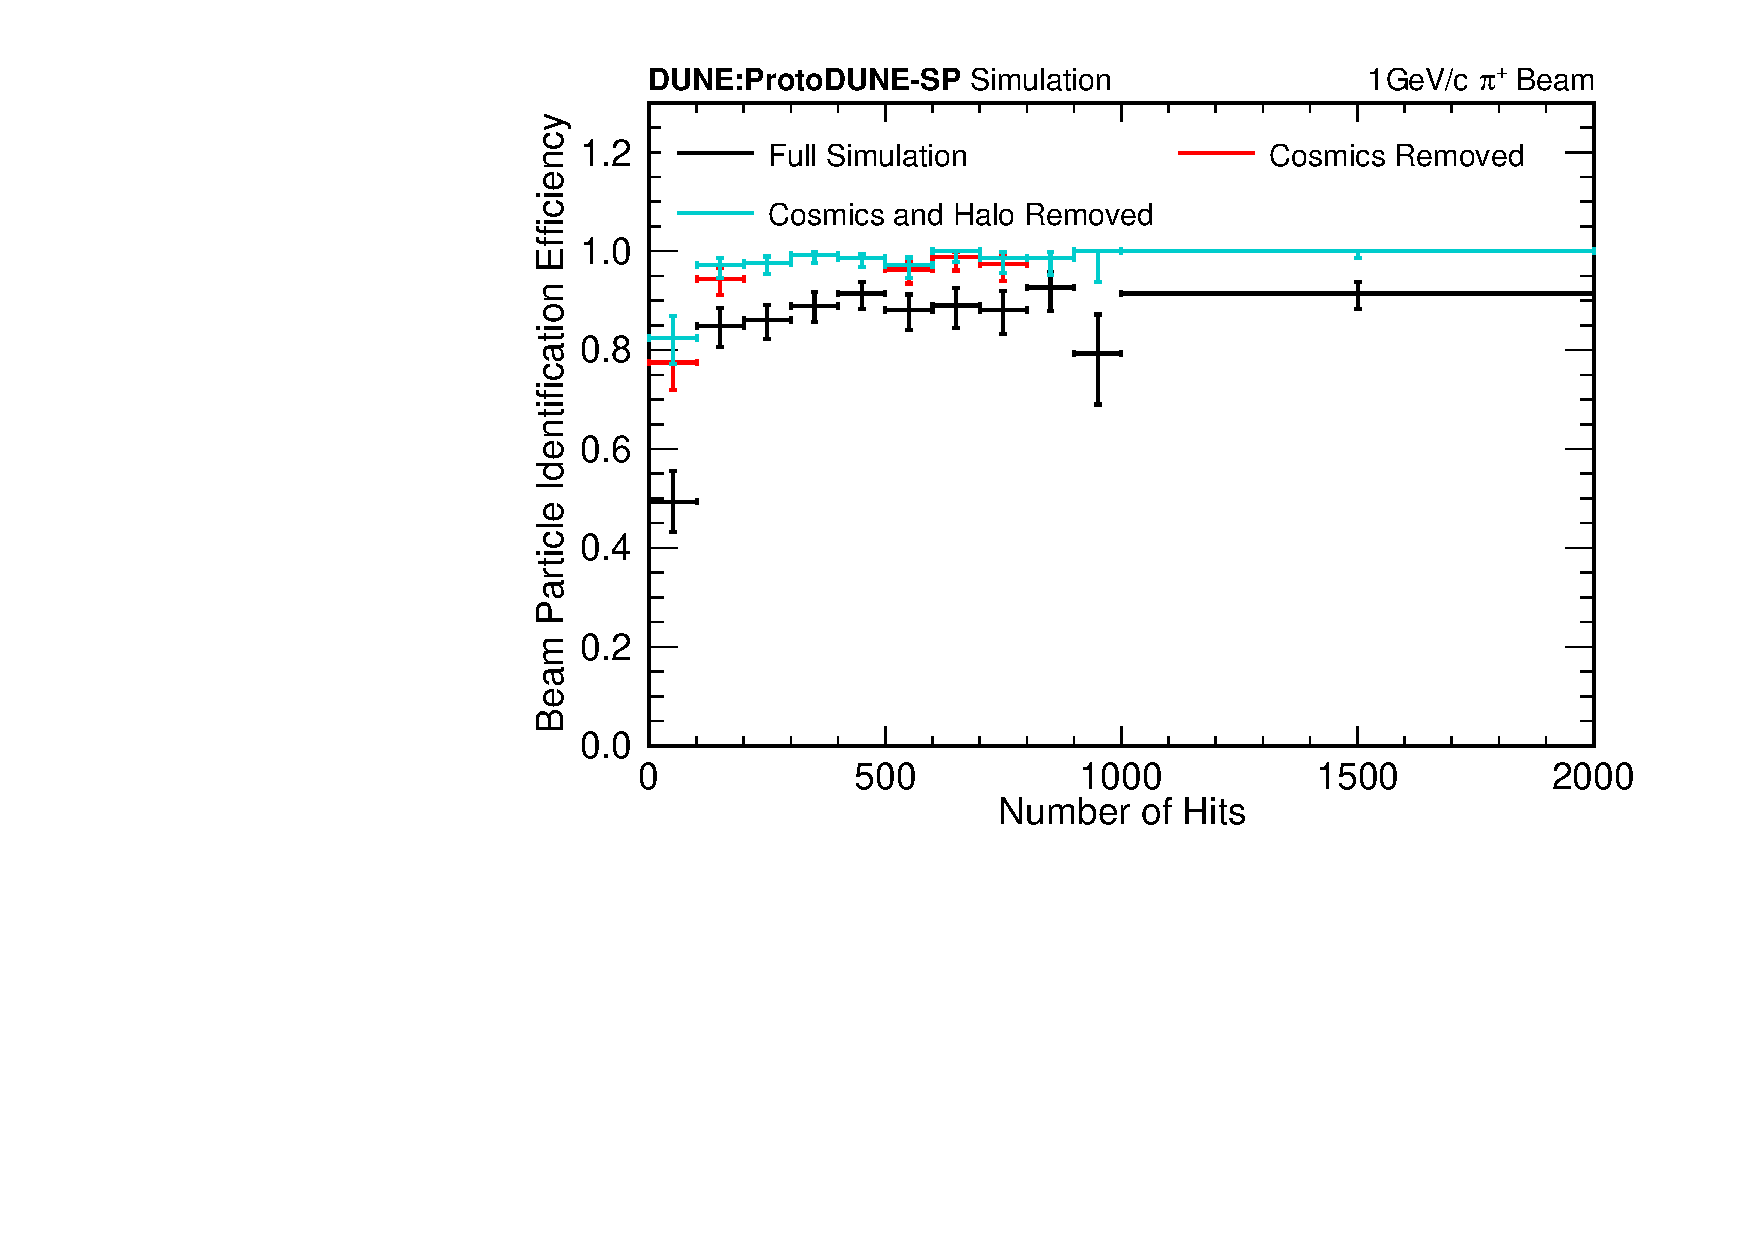
\includegraphics[width=0.48\textwidth,trim={0 0 0.5cm 0},clip]{Figures/Metrics/MC/Beam/Breakdown/BeamParticleEfficiencyVsNHitsPiPlus.pdf}
  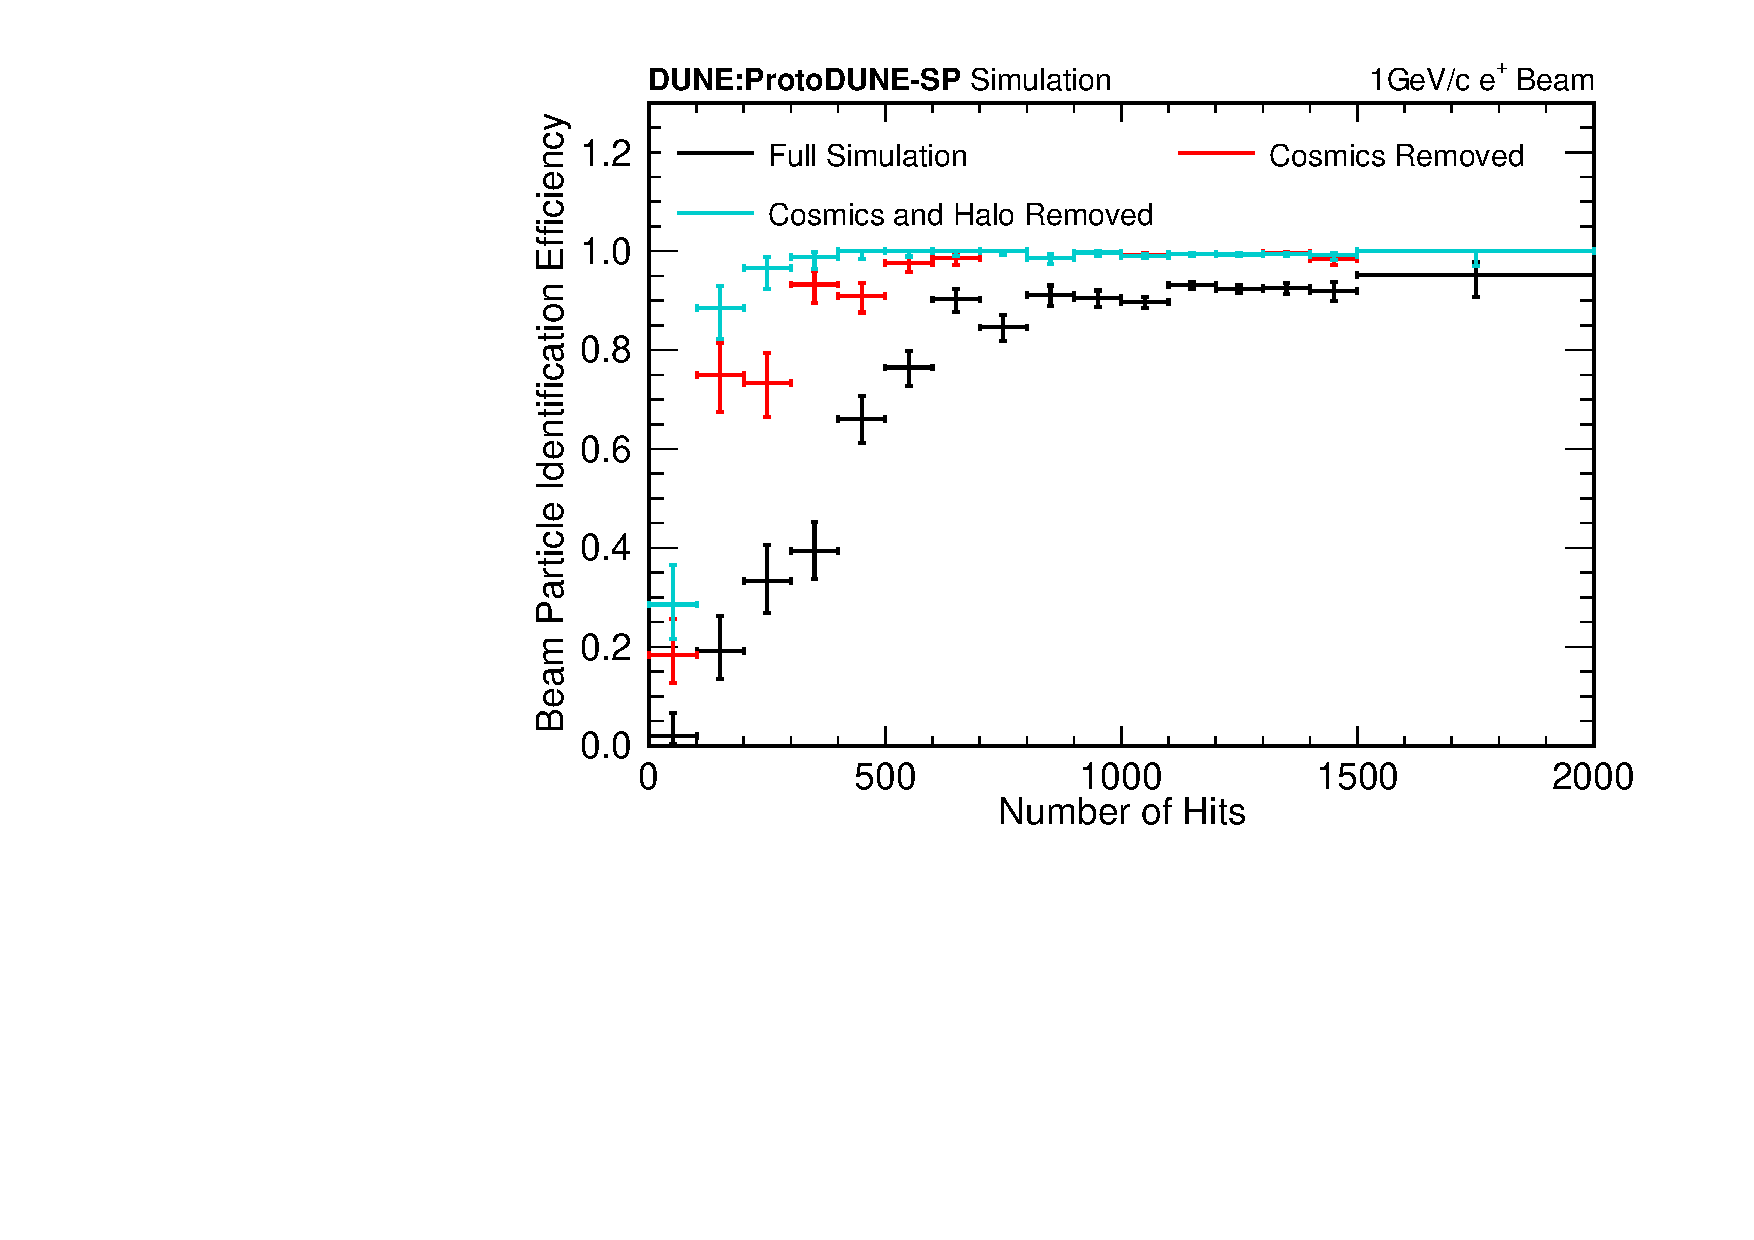
\includegraphics[width=0.48\textwidth,trim={0 0 0.5cm 0},clip]{Figures/Metrics/MC/Beam/Breakdown/BeamParticleEfficiencyVsNHitsPositron.pdf} \\
  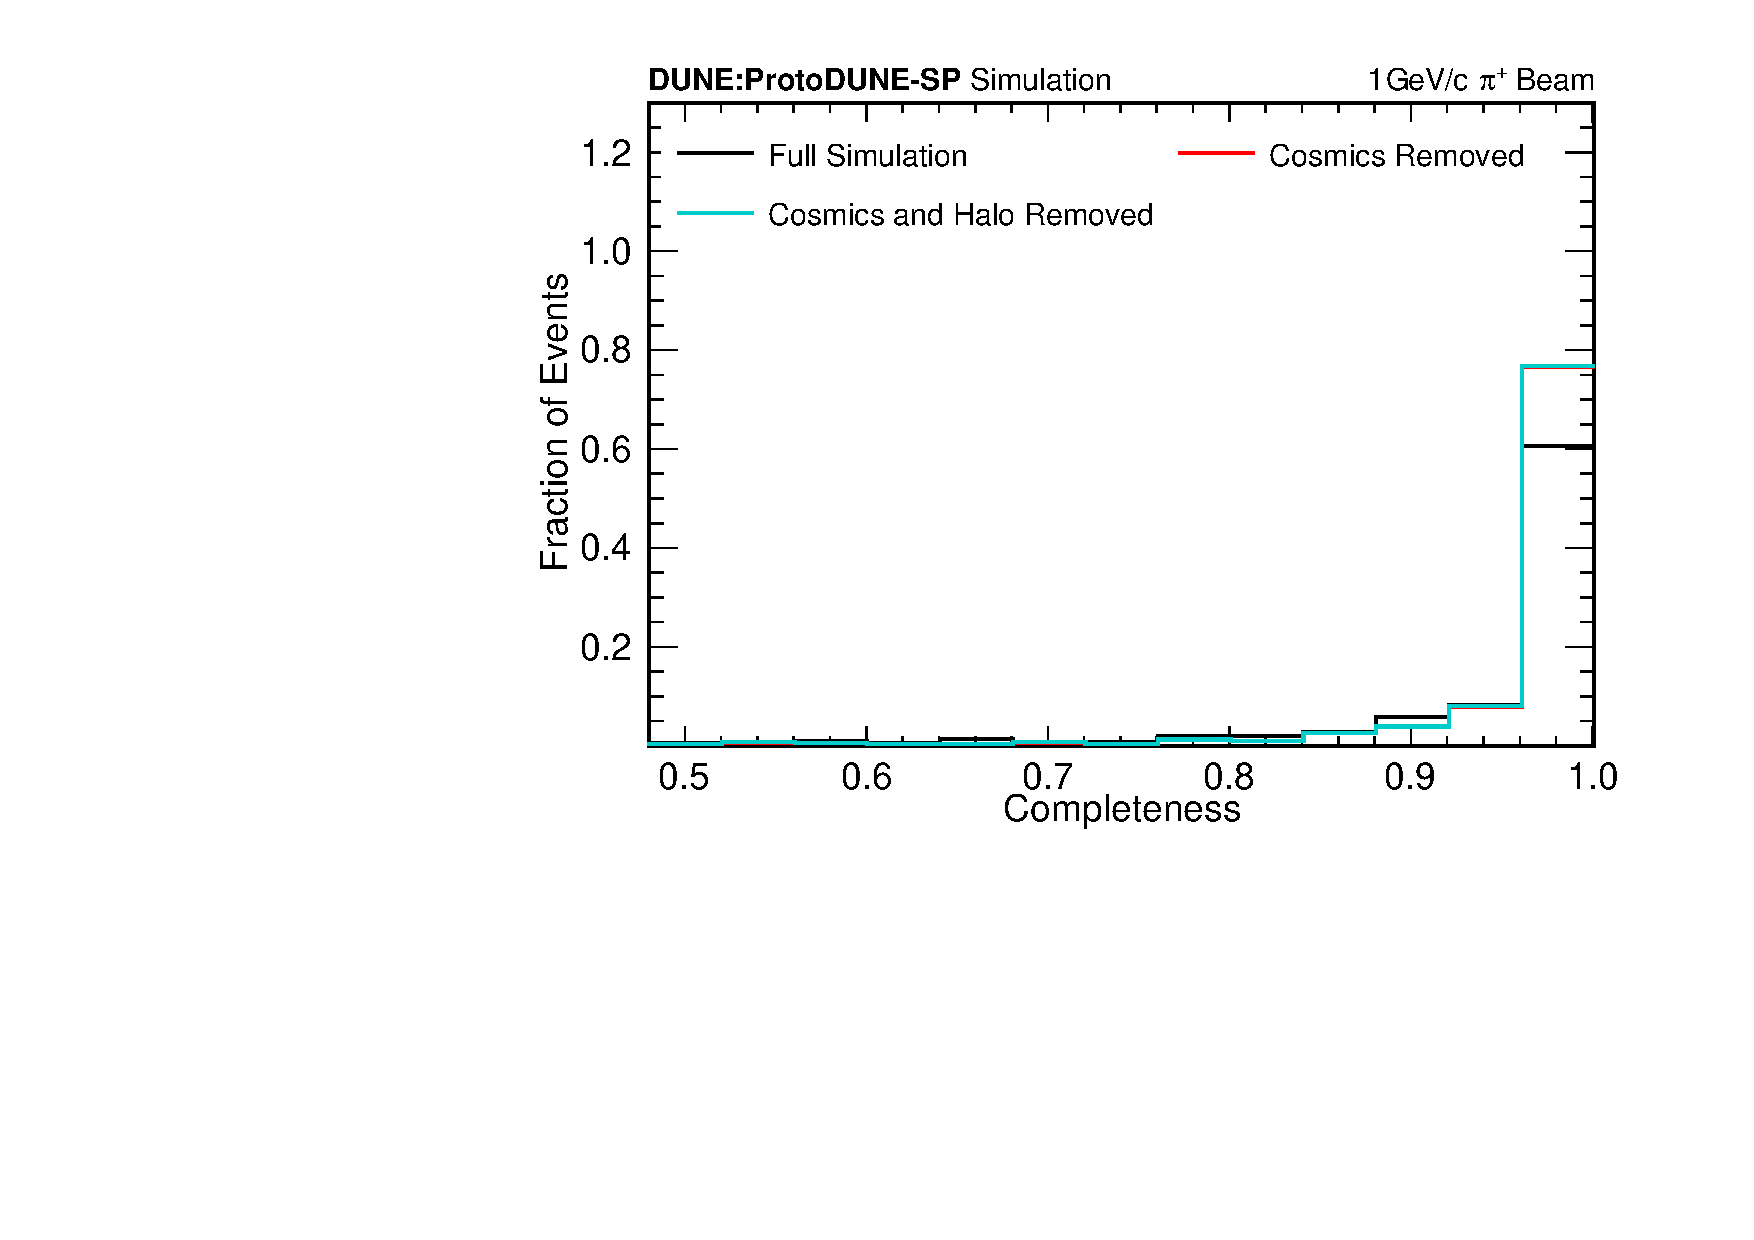
\includegraphics[width=0.48\textwidth,trim={0 0 0.5cm 0},clip]{Figures/Metrics/MC/Beam/Breakdown/BeamParticleCompletenessPiPlus.pdf}
  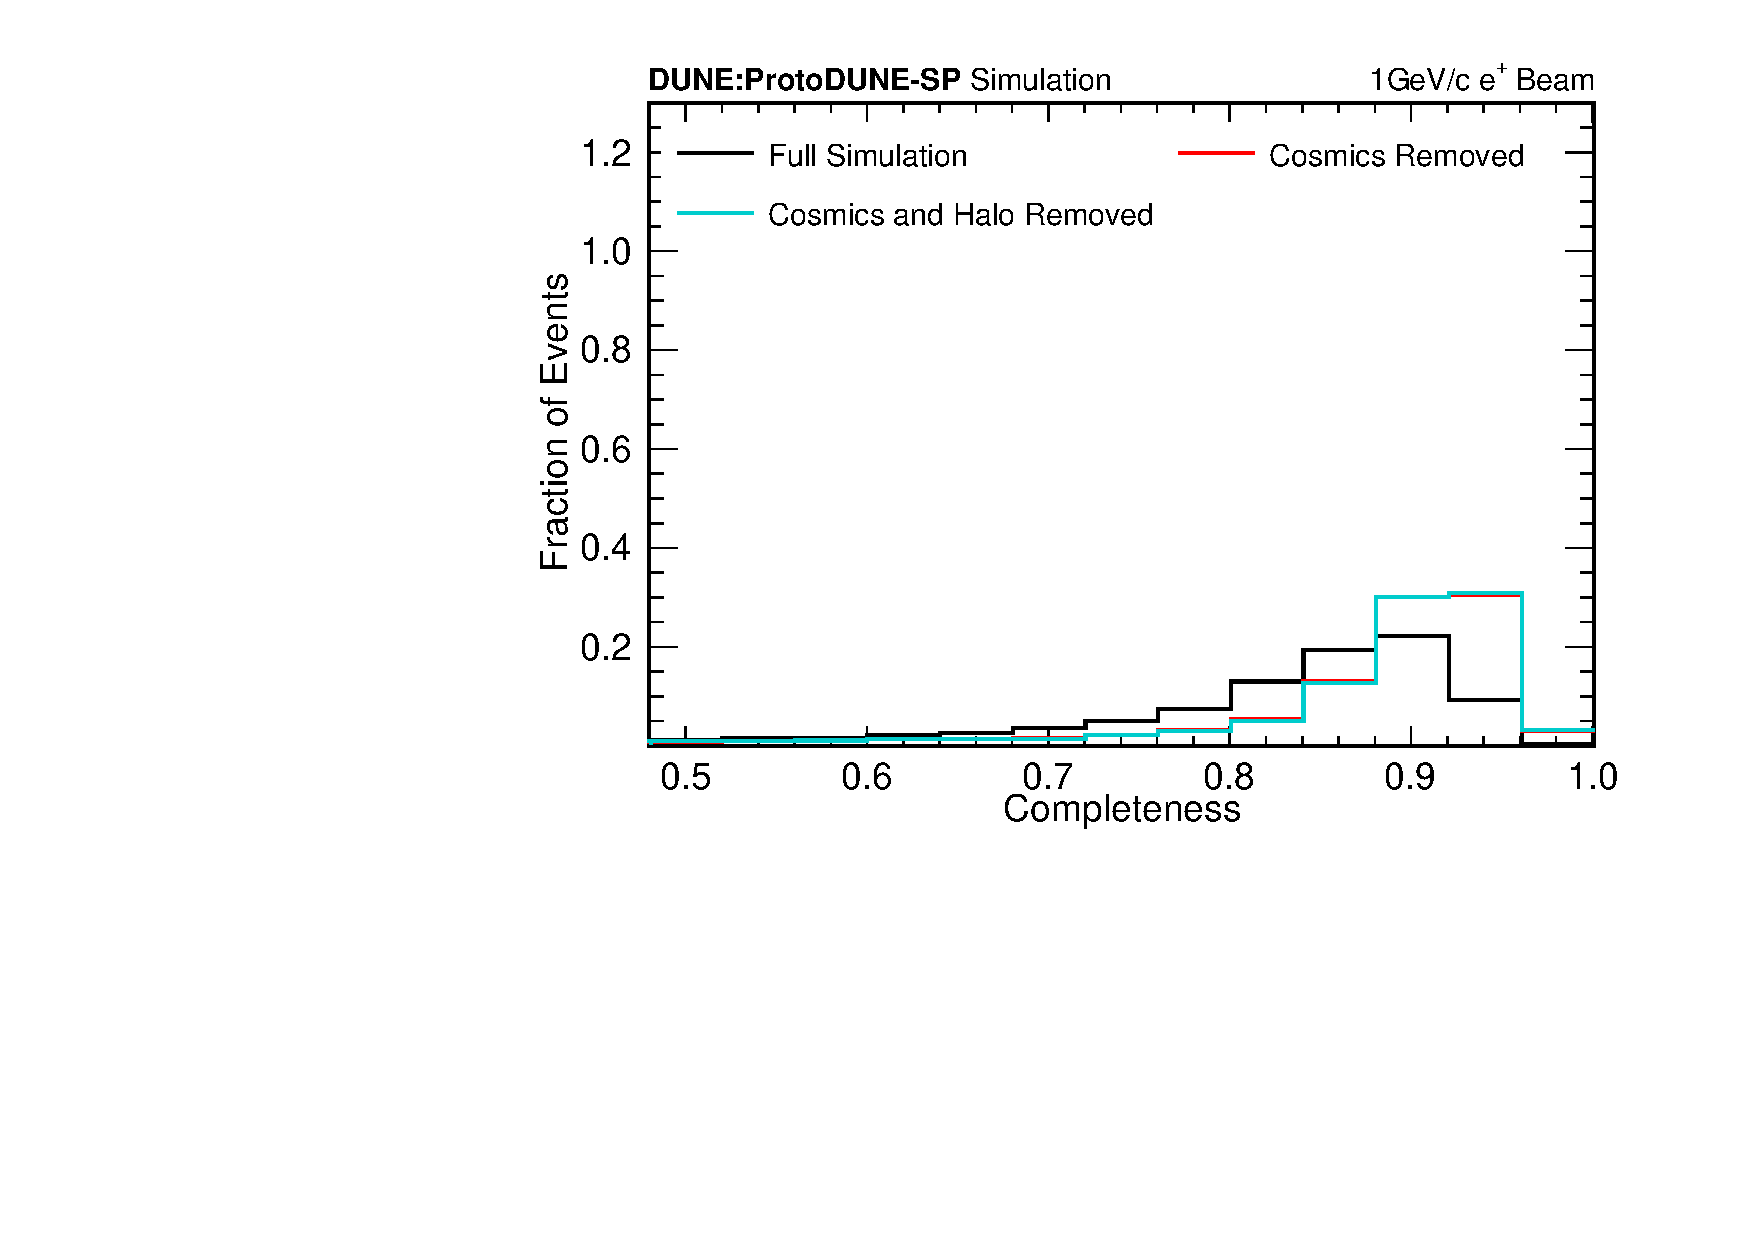
\includegraphics[width=0.48\textwidth,trim={0 0 0.5cm 0},clip]{Figures/Metrics/MC/Beam/Breakdown/BeamParticleCompletenessPositron.pdf}
  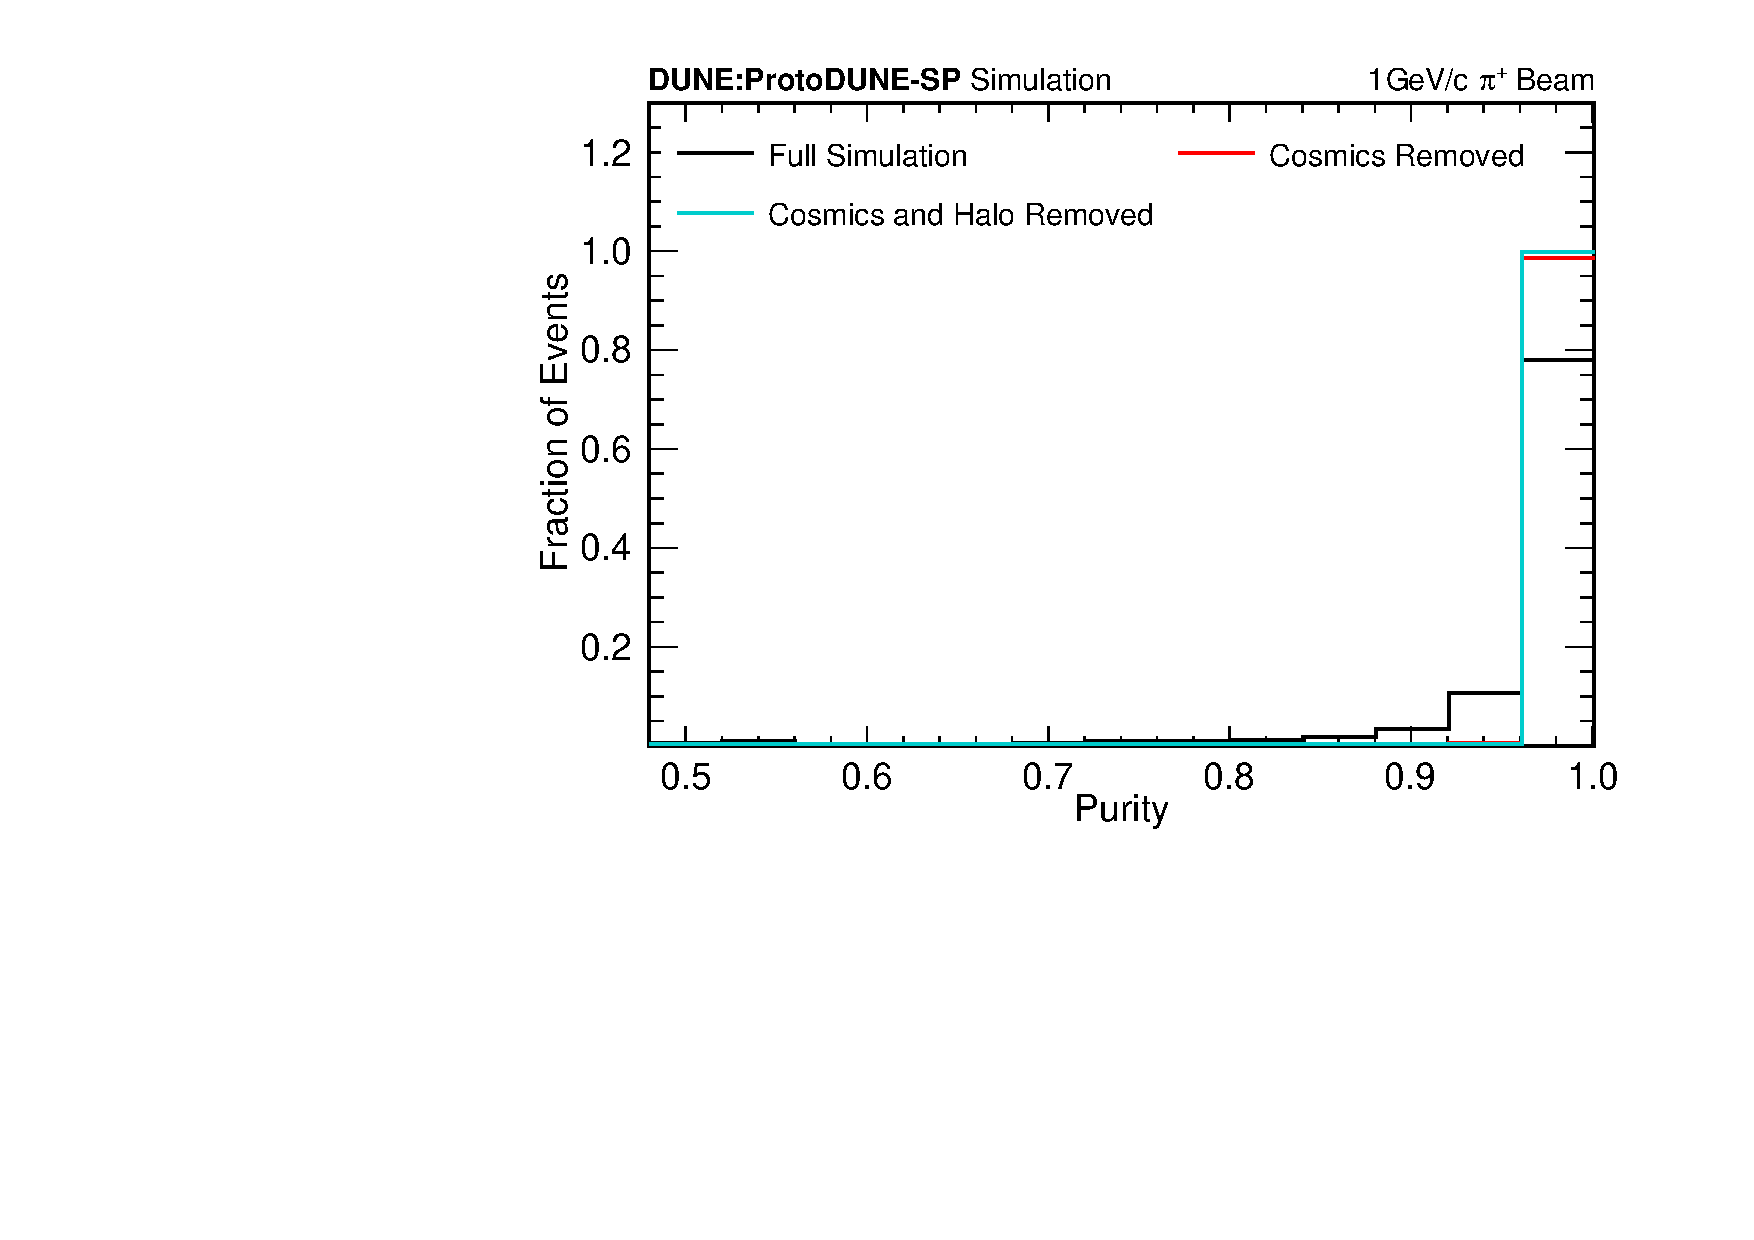
\includegraphics[width=0.48\textwidth,trim={0 0 0.5cm 0},clip]{Figures/Metrics/MC/Beam/Breakdown/BeamParticlePurityPiPlus.pdf}
  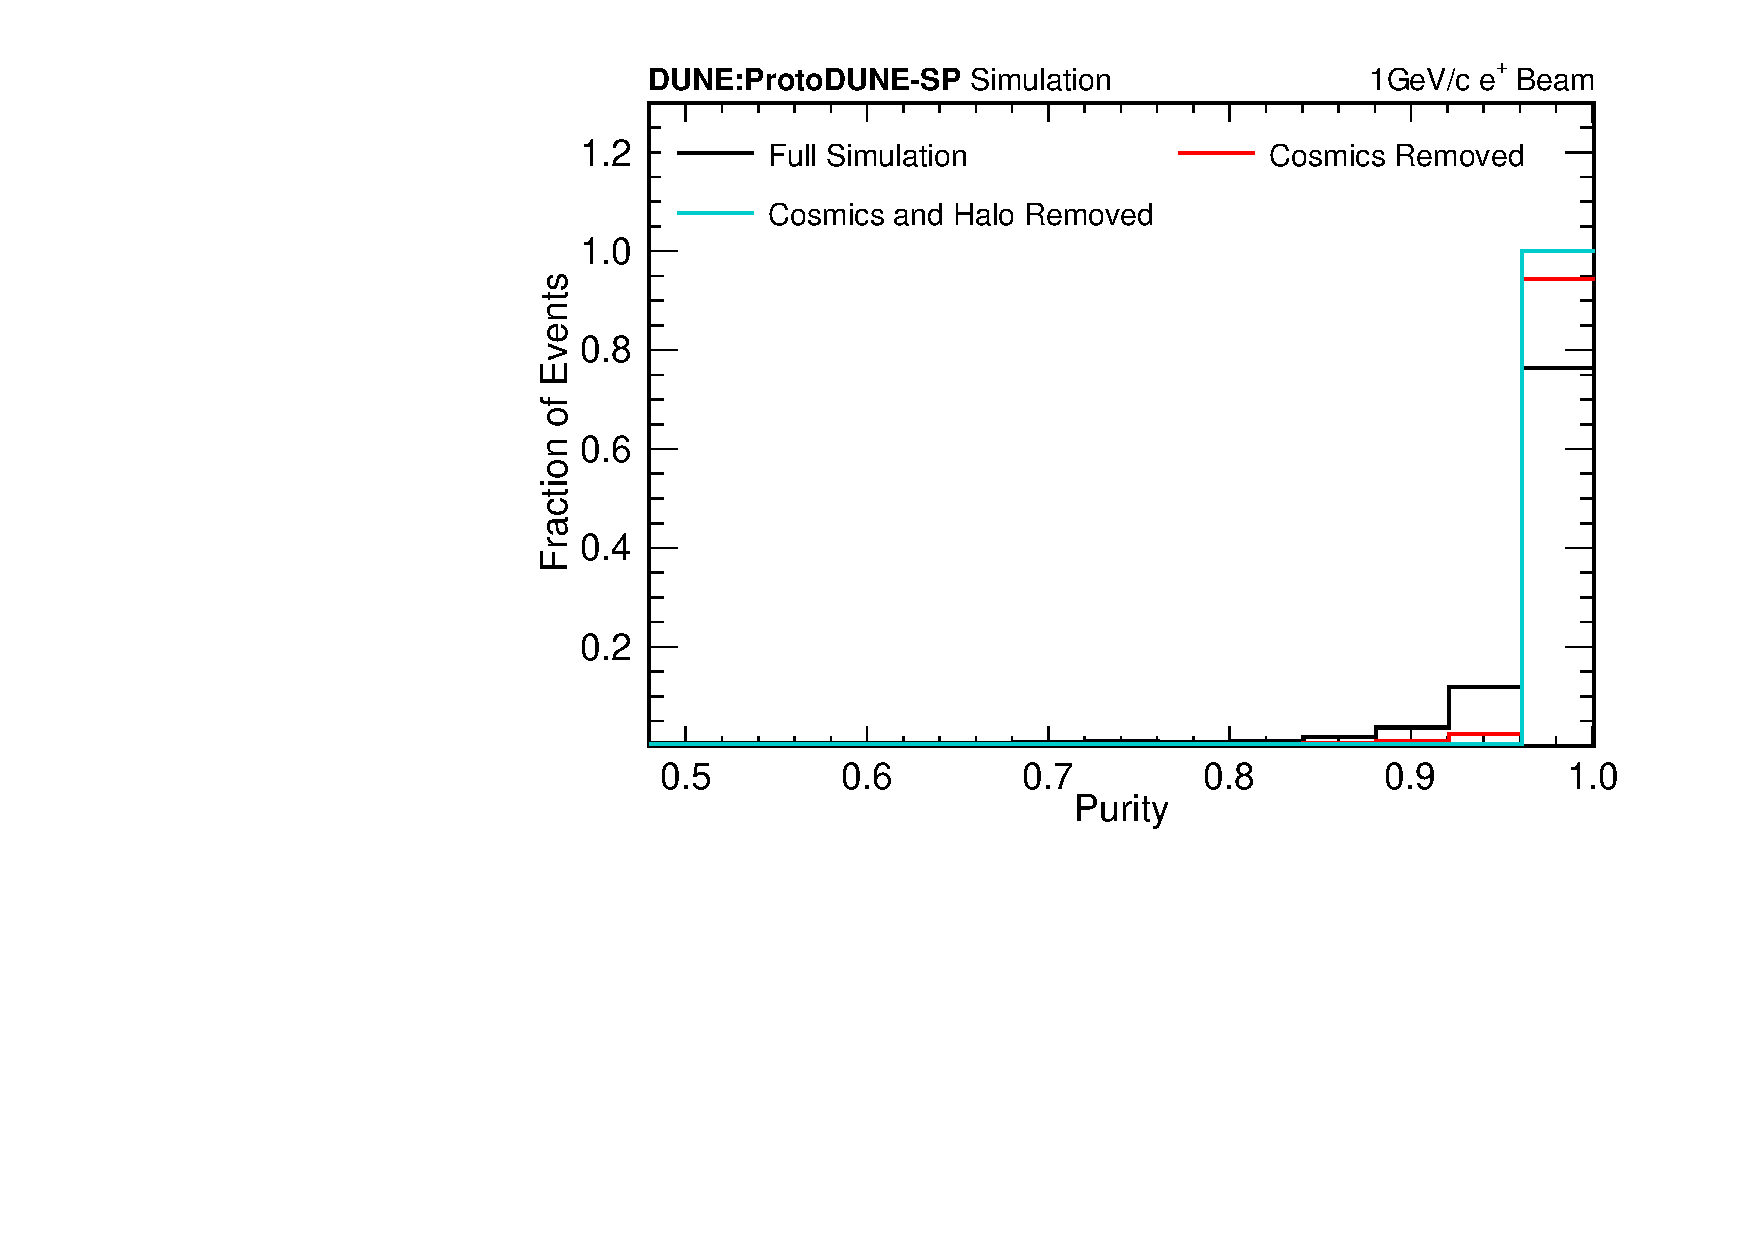
\includegraphics[width=0.48\textwidth,trim={0 0 0.5cm 0},clip]{Figures/Metrics/MC/Beam/Breakdown/BeamParticlePurityPositron.pdf}
\caption{Primary beam particle reconstruction and identification efficiency (top row) and the reconstructed particle completeness (middle row) and purity (bottom row) for 1\,GeV/$c$ $\pi^+$ (left column) and 1\,GeV/$c$ $e^+$ (right column) beam. The black distributions show the performance for the full ProtoDUNE-SP simulation, and the red and cyan curves show events with no cosmic rays, and no cosmic rays and no beam halo, respectively. In a number of places the red distribution is exactly covered by the cyan points.}
\label{fig:tbrecoeffbrkdwn}
\end{figure*}

The top figures show the reconstruction and identification efficiency for the triggered test-beam particles as a function of the number of 2D hits they produce in the detector (including hits produced by their interaction and decay products). The efficiencies for the full simulation both increase as a function of the number of hits and eventually plateau at $\sim$\,90\% for charged pions and $\sim$\,95\% for positrons. Removing cosmic-ray muons from the simulation significantly increases the efficiency over the whole range of the number of hits. At 1\,GeV/$c$ there are few beam halo particles, so only a small efficiency increase is seen after the sequential removal of the beam halo. As expected, the efficiency is approximately 100\% after the removal of all background particles, demonstrating that the performance on the full simulation is limited by the physics of the interactions and complex overlapping topologies. Similar behaviour is seen for the other beam particle types and the different momentum setting values. The average reconstruction and identification efficiency of the full simulation sample, for all particle types and beam momentum settings, is given in Table~\ref{tab:beamsimeff} and shown graphically in Fig.~\ref{fig:beam_efficiency}. There are more beam halo particles in the 6 and 7\,GeV/$c$ beam samples, which reduce the efficiency for charged pions and protons because they can be hidden within a beam halo positron shower. The efficiency remains high for high-energy positrons since they produce very large electromagnetic showers. 

\begin{table*}[htb]
\centering
\caption{The reconstruction and identification efficiency for the triggered test-beam particle in ProtoDUNE-SP simulation for positrons, charged pions, protons and charged kaons for different beam momenta. Charged kaons are negligible in number from 1 to 3\,GeV/$c$. The simulated events include the triggered test-beam particle, beam halo particles and numerous cosmic rays.}
\label{tab:beamsimeff} 
\begin{tabular}{cccccc}
\hline\noalign{\smallskip}
Momentum & \multicolumn{5}{c}{Reconstruction Efficiency $\left[\textrm{\%}\right]$} \\
$\left[\textrm{GeV/$c$}\right]$ & Positrons $\left(e^+\right)$& Pions $\left(\pi^+\right)$ & Protons $\left(p\right)$& Kaons $\left(K^+\right)$& Muons $\left(\mu^+\right)$\\
\noalign{\smallskip}\hline\noalign{\smallskip}
1 & 88.0$^{+0.2}_{-0.2}$ & 86.1$^{+0.6}_{-0.6}$ & 84.1$^{+0.6}_{-0.6}$ & -- & 88.6$^{+2.1}_{-2.5}$\\
2 & 89.9$^{+1.2}_{-1.3}$ & 87.3$^{+1.3}_{-1.5}$ & 86.8$^{+1.9}_{-2.1}$ & -- & 100.0$^{+0.0}_{-9.2}$\\
3 & 90.5$^{+1.1}_{-1.2}$ & 87.5$^{+0.5}_{-0.5}$ & 86.1$^{+1.1}_{-1.2}$ & -- & 94.0$^{+2.2}_{-3.1}$\\
6 & 90.9$^{+0.9}_{-1.0}$ & 78.8$^{+0.6}_{-0.6}$ & 78.9$^{+1.8}_{-1.9}$ & 80.7$^{+2.5}_{-2.7}$ & 94.0$^{+2.2}_{-3.5}$\\
7 & 92.1$^{+1.0}_{-1.1}$ & 75.3$^{+0.9}_{-1.0}$ & 73.8$^{+2.6}_{-2.8}$ & 78.3$^{+3.4}_{-3.8}$ & 85.7$^{+5.5}_{-7.6}$\\
\noalign{\smallskip}\hline
\end{tabular}
\end{table*}

\begin{figure}[htb]
\centering
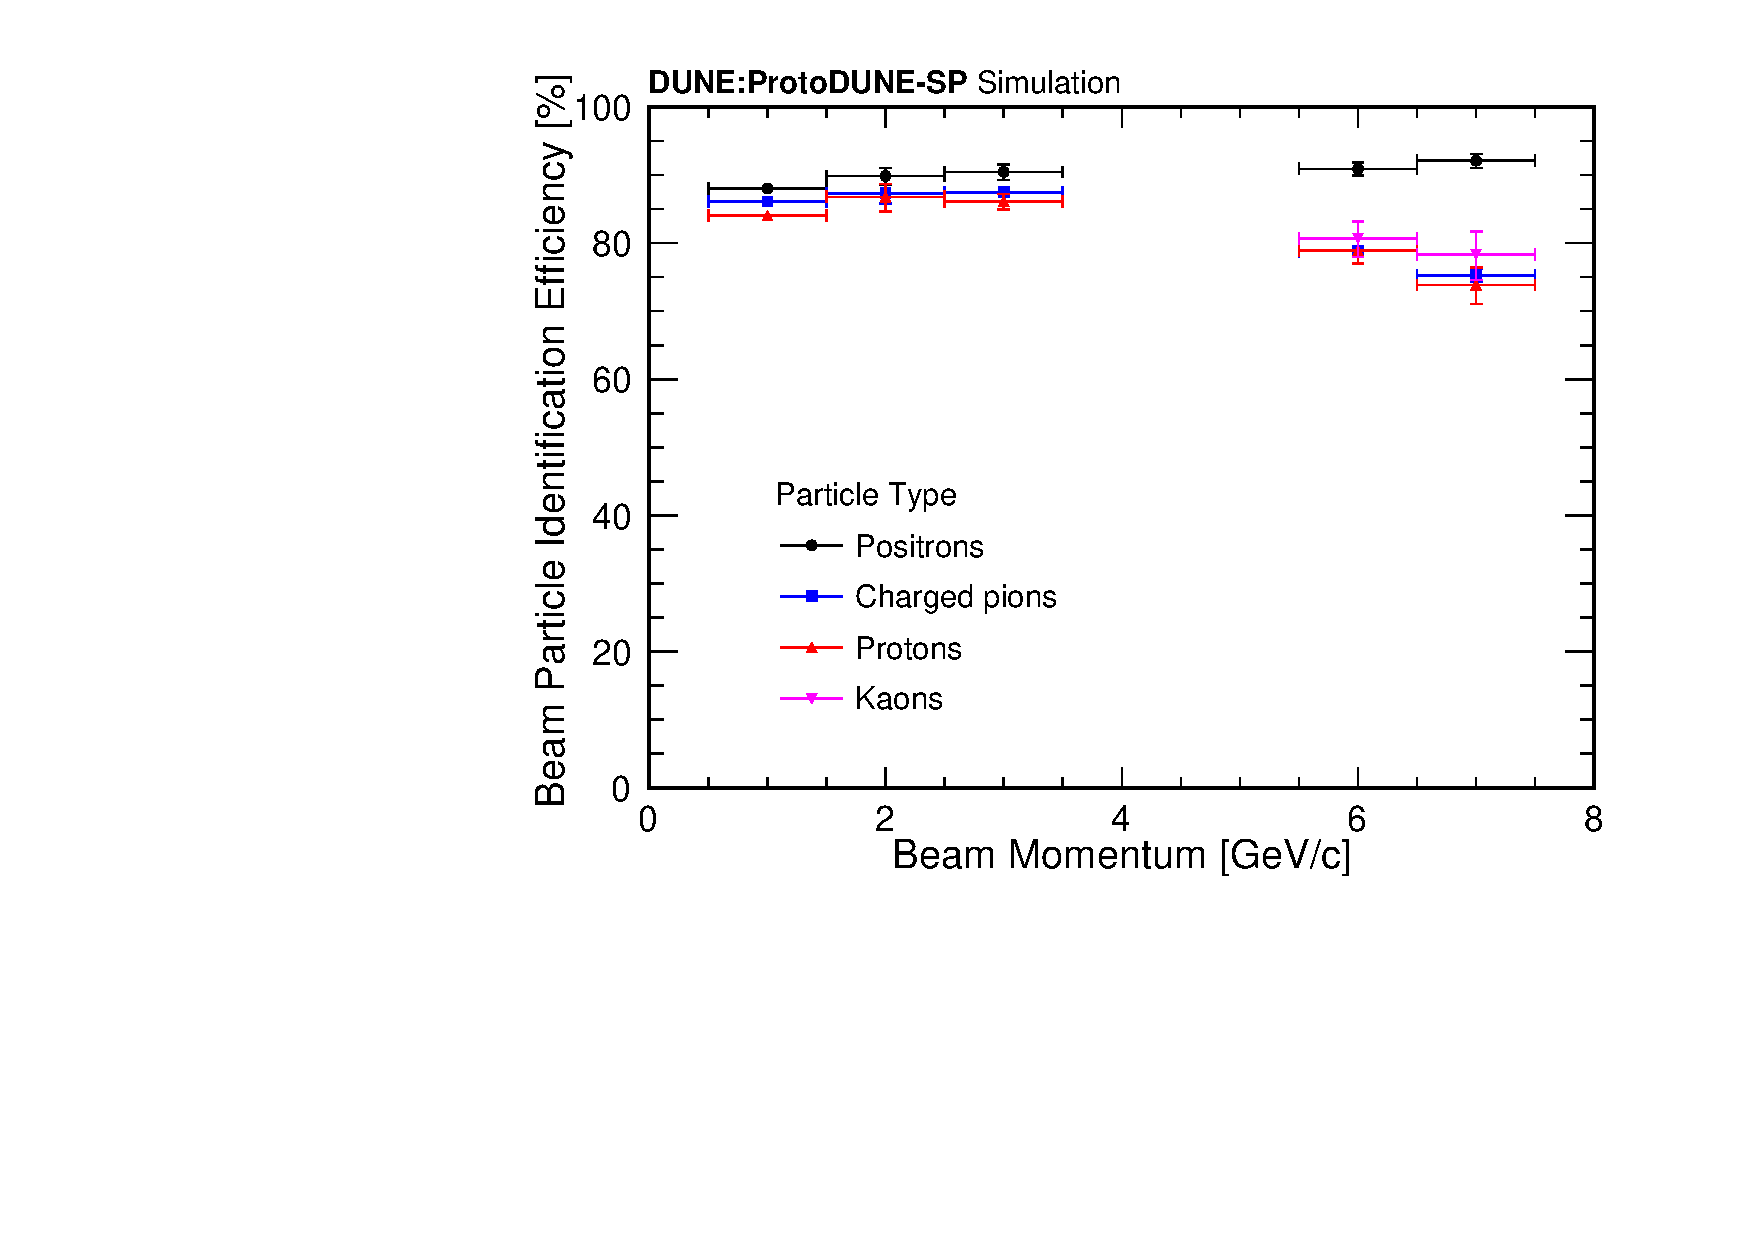
\includegraphics[width=0.65\textwidth]{Figures/Metrics/MC/Beam/prod2_newBDT_beam_eff.pdf}
\caption{The beam particle identification efficiency for the test-beam particle in ProtoDUNE-SP simulation for different beam momenta. Data was not collected at 4\,GeV/$c$ or 5\,GeV/$c$, so no entries are shown for these momenta. For clarity, antimuons are not shown due to their large statistical uncertainty.}
\label{fig:beam_efficiency}
\end{figure}

The middle and bottom rows of Fig.~\ref{fig:tbrecoeffbrkdwn} show the completeness and purity of the reconstructed test-beam particle hierarchy, respectively. The four distributions are peaked at, or close to, one, indicating that the triggered test-beam particle is being reconstructed as a single, complete particle. Removing the cosmic-ray muons significantly improves both completeness and purity of the test-beam particle reconstruction. This improvement is expected as there are fewer hits to contaminate the reconstructed beam slice, or to incorrectly split the reconstructed beam particle in the slicing algorithm. Removing both cosmic-ray muons and beam halo particles enforces a purity of 100\% as all possible sources of contamination have been removed, and there is a small increase in the completeness. The effect of removing the cosmic rays is larger, which is to be expected as there are significantly more cosmic rays than beam halo particles, such that the slicing algorithm, a source of incomplete triggered test-beam particles, is less active for events where cosmic-ray muons have been removed irrespective of the presence of the second-order beam halo effect.

\subsection{Comparison of Data and Simulation}
\label{sec:data}

In order to compare the triggered test-beam particle reconstruction and identification efficiency between data and MC, a less strict definition of efficiently reconstructed test-beam particles is used in comparison to the one described in Section~\ref{sec:beam_mc}. The following selection is used to obtain the sample of events that are highly likely to contain a beam particle, and hence form the denominator for the efficiency calculation.

\begin{itemize}
\item[]Data:
\begin{enumerate}
  \item The beam trigger is active.
  \item A single track is reconstructed in the beam monitors immediately upstream of ProtoDUNE-SP.
  \item The detector high-voltage is stable at -180\,kV.
  \item The readout electronics on the beam-side of the detector are active.
  \item There are at least 10 3D hits in the region where the beam particle enters the detector. These 3D hits are reconstructed as part of the disambiguation procedure described in Sec.~\ref{sec:patrec}, not by Pandora.
\end{enumerate}
\item[] Simulation:
\begin{enumerate}
  \item There is a triggered test-beam particle in the MC particle hierarchy
  \item There are at least 10 3D hits in the region where the beam particle enters the detector.
\end{enumerate}
\end{itemize}
The efficiency is then defined as the fraction of the selected events with a reconstructed beam particle hierarchy. 

There are some limitations in the ability of the beam instrumentation alone to give the unambiguous particle identification required to calculate the denominator of the reconstruction and identification efficiency. Pions and antimuons are not distinguished, and since triggered test-beam charged pions can decay in the beamline to antimuons, they are included as a joint sample. For the 6 and 7\,GeV/$c$ samples, positrons, charged pions and antimuons can not be distinguished, and are hence not included in the comparisons.\footnote{Physics analysis is possible as positrons are reconstructed as showers and can be easily selected. However, calculation of the absolute efficiency in data is not possible.} A summary of the momentum settings used for data and MC comparisons is as follows:
$\pi^{+}$/$\mu^+$ from 1 to 3\,GeV/$c$, $e^+$ from 1 to 3\,GeV/$c$, $p$ from 1 to 7\,GeV/$c$, and $K^+$ for 6 and 7\,GeV/$c$.

Two additional simulation samples were produced to investigate the effect of potential systematic uncertainties.
\begin{enumerate}
    \item The SCE-off sample does not have a simulation of the space charge effect. It gives an estimate of potential efficiency mismodelling due to differences in the SCE between data and MC. Since a sample with increased SCE was not available, the efficiency difference from using the SCE-off sample was used to produce a symmetric band around the standard simulation efficiency values.
    \item A sample with the beam halo component reduced by 15\%. This sample was motivated by Ref.~\cite{PhysRevAccelBeams.22.061003} that shows that the MC overestimates the beam trigger rate, and hence the event pileup. The difference between the efficiency measured from the standard simulation and this sample was taken as a symmetric systematic uncertainty centred on the standard simulation efficiency.
\end{enumerate}

Furthermore, to account for potential differences in the 3D hit finding between data and MC, the selection criterion requiring 10 3D hits in the region where the beam enters the detector was varied for the simulation to 8 and 12 and the change in efficiency was taken as a systematic uncertainty, giving the higher and lower limits on the systematic uncertainty band, respectively. This variation only has a significant effect for the 1\,GeV/$c$ sample because the low energy particles produce fewer hits than those at higher energies. The total systematic uncertainty is calculated as the quadrature sum of the aforementioned individual systematic uncertainties.

Figure~\ref{fig:datamcrecoeff} shows the reconstruction and identification efficiency for triggered test-beam charged pions, positrons, protons and kaons as a function of the beam momentum setting. The simulation is shown with statistical uncertainties (darker red) and the quadrature sum of statistical and systematic uncertainties (pale red).

\begin{figure*}[htb]
\centering
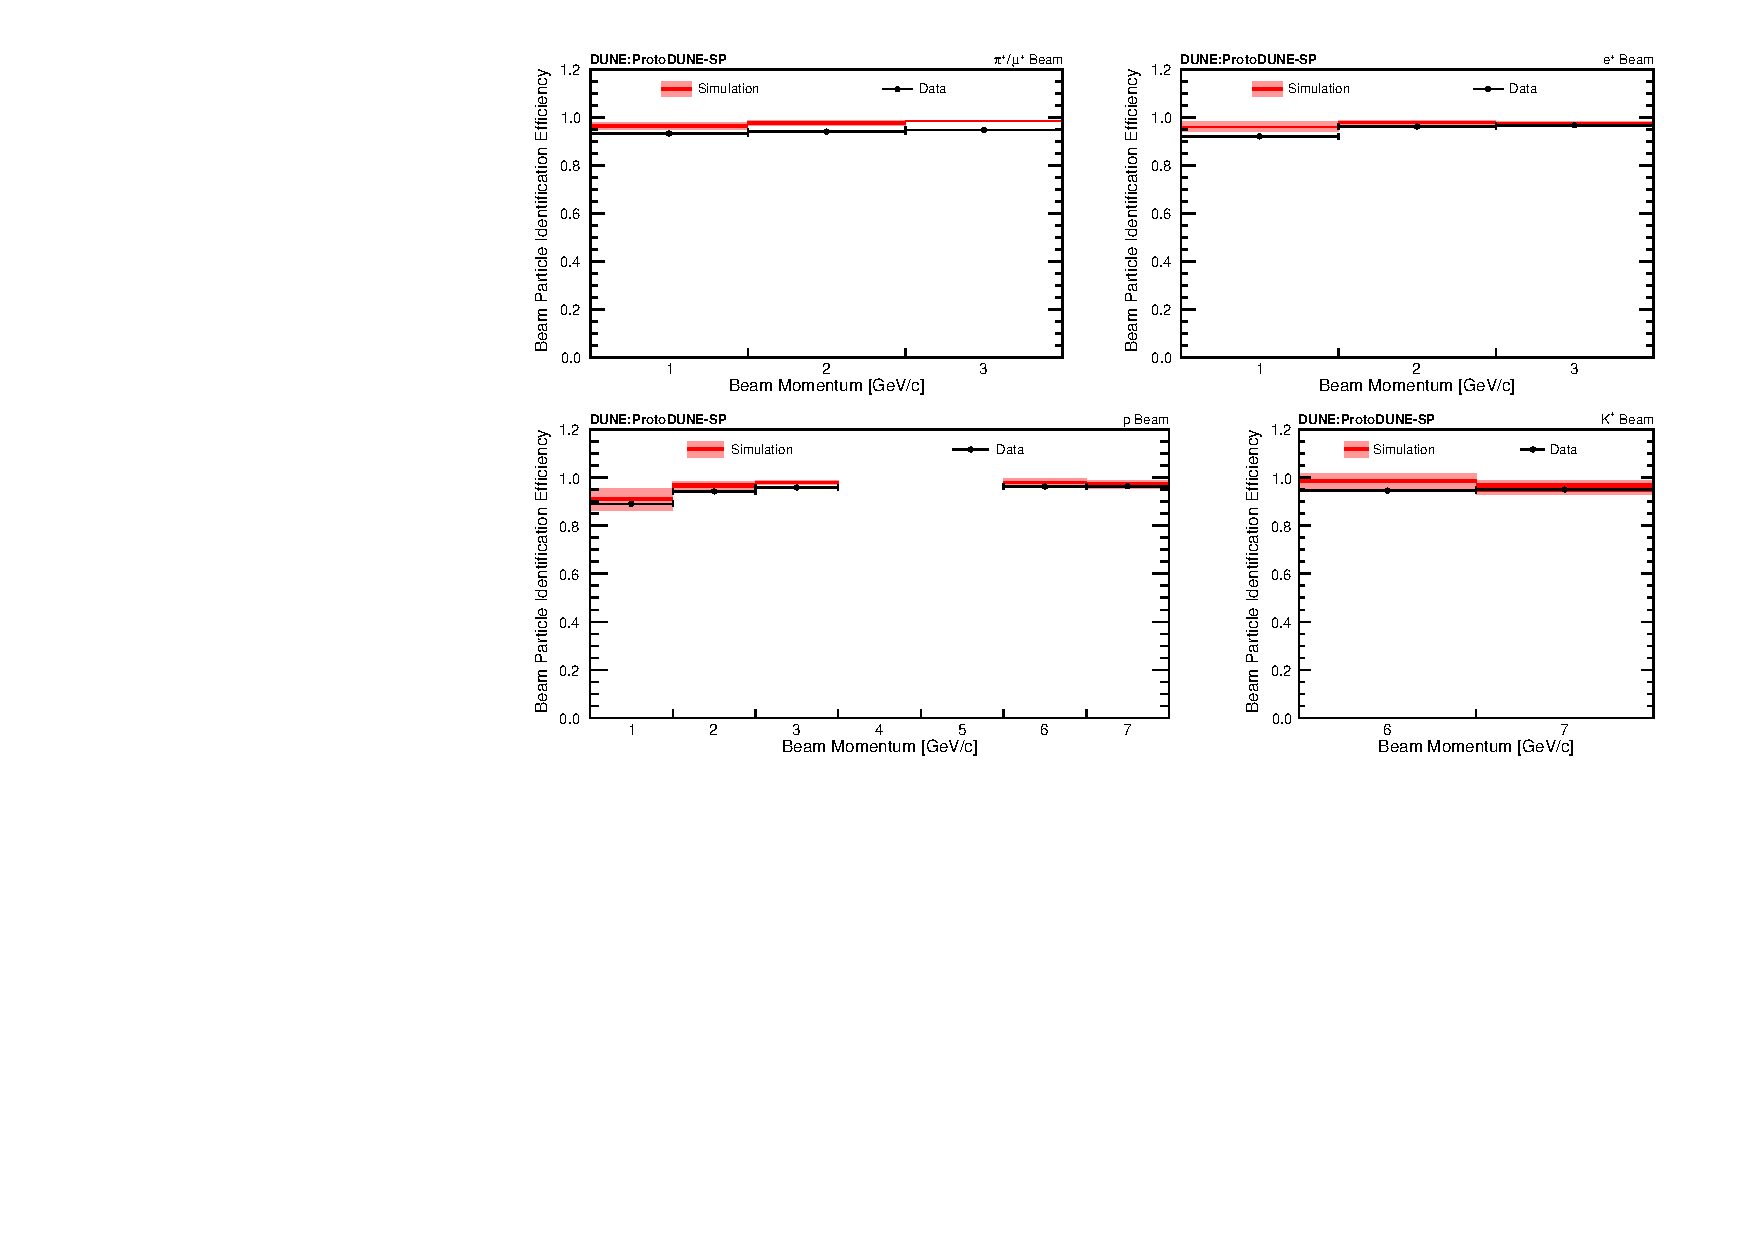
\includegraphics[width=0.98\textwidth,trim={0 0 0.5cm 0},clip]{Figures/Metrics/Data/Beam/prod2_pandora_data_mc_all_effs_bin.pdf}
\caption{The triggered test-beam particle reconstruction efficiency for ProtoDUNE-SP as a function of the beam momentum in data and simulation, for charged pions and antimuons (top left), positrons (top right), protons (bottom left) and charged kaons (bottom right). The pale red simulation band shows the total uncertainty and the statistical-only uncertainty is shown in dark red.}
\label{fig:datamcrecoeff}
\end{figure*}

Agreement is seen between the data and simulation and any discrepancies are within 5\%. As expected, the lowest efficiency is seen at 1\,GeV/$c$ where the particles deposit the least energy in the detector. In particular, 1\,GeV/$c$ protons are the most difficult to reconstruct since they travel the shortest distance within the detector.

The fraction of events with a reconstructed beam slice for the pion/muon sample is slightly overestimated in MC compared to data. A number of factors could cause this behaviour. The SCE is underestimated in the simulation~\cite{proto_performance}, which means that the reconstructed beam slices are slightly easier to identify in the simulation. Furthermore, the ratio of muons to pions can differ between data and MC but it is not possible to distinguish these two types of particles due to their similar masses, and a difference in the reconstruction efficiency between pions and muons will induce a data vs MC discrepancy. Finally, in the experimental data, there is a higher probability that beam pion and muon tracks will be broken at the boundary between the first two APAs due to the presence a malfunctioning electron diverter~\cite{proto_performance} that distorts the electric field, which could cause a small reduction in efficiency. Newer versions of the simulation will account for these three effects. However, small differences in the integrated efficiency between data and MC do not have a big impact for the cross-section analyses because the overall normalisation cancels in the cross-section calculation.

\section{Conclusions}
\label{sec:conclusion}
A summary of Pandora, a pattern-recognition software package, has been presented alongside relevant modifications allowing it to be applied to simulated and experimental data interactions in the ProtoDUNE-SP LArTPC detector. Pandora is the primary event reconstruction used in all ProtoDUNE-SP physics analyses and enables the measurement of hadronic cross sections on liquid argon, the primary physics goal of the experiment. The performance of Pandora has been extensively evaluated for simulated charged test-beam and cosmic-ray interactions in the ProtoDUNE-SP detector. Several pattern-recognition metrics have been evaluated enabling a comparison of data and simulation.

The efficiency to reconstruct the triggered test-beam particle and correctly identify it as of beam origin exceeds 80\% for the majority of particle types ($e^+$, $\pi^+$, $p$, $K^+$, $\mu^+$) and momentum setting combinations (1, 2, 3, 6 and 7\,GeV/$c$). It was also shown that the main cause of these inefficiencies arises from background contamination from both cosmic and beam-halo sources. In background-removed simulation samples the triggered test-beam particle reconstruction and identification efficiency is almost 100\% in all cases. A comparison of data and MC shows agreement within 5\% for the reconstruction and identification efficiency for different triggered beam-particle species across the beam momentum values, and possible sources for the small observed efficiency differences were discussed.

Over the coming years, developments to the pattern-recognition are expected from the introduction of new algorithms and the incorporation of deep-learning techniques to drive some key decisions within the Pandora multi-algorithm approach. Examples include improved vertex finding, event slicing and hit classification. Whilst many of these new algorithms are being developed for the DUNE FD, they will be tested on the ProtoDUNE-SP simulation and data. ProtoDUNE-SP has been dismantled but a very similar upgraded detector called ProtoDUNE-HD is under construction in the same cryostat, which is due to commence data taking at the end of 2022.

\begin{acknowledgements}
% \documentclass{article}
% \usepackage[utf8]{inputenc}

% \begin{document}

% \centerline{\bf DUNE Acknowledgement}
% \centerline{\bf January 2022}
% \bigskip

% Below is a standard paragraph to be included in DUNE publications. 
% The sentences acknowledging Fermilab and funding agencies should always appear. 
% The sentences relevant to ProtoDUNE would appear only in ProtoDUNE papers. 
% The sentence acknowledging NERSC should appear only in papers that used NERSC resources.
% \bigskip \hrule \bigskip

%
% Acknowledgement of CERN for ProtoDUNE construction and operations
%
The ProtoDUNE-SP detector was constructed and operated on the CERN Neutrino Platform.
We gratefully acknowledge the support of the CERN management, and the
CERN EP, BE, TE, EN and IT Departments for NP04/Proto\-DUNE-SP.
%
% Standard piece for all FNAL-based experiments
%
This document was prepared by the DUNE collaboration using the
resources of the Fermi National Accelerator Laboratory 
(Fermilab), a U.S. Department of Energy, Office of Science, 
HEP User Facility. Fermilab is managed by Fermi Research Alliance, 
LLC (FRA), acting under Contract No. DE-AC02-07CH11359.
%
% Funding agencies, alphabetical by country, then alphabetical by agency name
%
This work was supported by
CNPq,
FAPERJ,
FAPEG and 
FAPESP,                         Brazil;
CFI, 
IPP and 
NSERC,                          Canada;
CERN;
M\v{S}MT,                       Czech Republic;
ERDF, 
H2020-EU and 
MSCA,                           European Union;
CNRS/IN2P3 and
CEA,                            France;
INFN,                           Italy;
FCT,                            Portugal;
NRF,                            South Korea;
CAM, 
Fundaci\'{o}n ``La Caixa'',
Junta de Andaluc\'ia-FEDER,
MICINN, and
Xunta de Galicia,               Spain;
SERI and 
SNSF,                           Switzerland;
T\"UB\.ITAK,                    Turkey;
The Royal Society and 
UKRI/STFC,                      United Kingdom;
DOE and 
NSF,                            United States of America.
%
% Acknowledgement of NERSC if those resources were used
%
This research used resources of the 
National Energy Research Scientific Computing Center (NERSC), 
a U.S. Department of Energy Office of Science User Facility 
operated under Contract No. DE-AC02-05CH11231.
%
%\end{document}

\end{acknowledgements}

\bibliographystyle{unsrtnat}
\bibliography{refs.bib}

\end{document}
